%%%%%%%%%%%%%%%%%%%%%%%%%%%%%%%%%%%%%%%%%%%
\documentclass[%
%underprogress,%
%showcomments,%
%noexperiments,% 
%externaltikz,%
%noindex,%
%margnum,%
%titles,%
openright%
]{settings/UUThesisTemplate}
%%%%%%%%%%%%%%%%%%%%%%%%%%%%%%%%%%%%%%%%%%%

\newcommand{\bjcom}[1]{\textcolor{blue}{\sl [#1]}}
\newcommand{\bjfix}[2]{{\sl [\textcolor{red}{#1} -> \textcolor{green}{#2}]}}
\newcommand{\bjcor}[1]{{\sl [\textcolor{red}{should be} \textcolor{green}{``#1''}]}}


\newcommand{\authorSurname}{Haziza}
\newcommand{\authorFirstName}{Frédéric}
\newcommand{\authorFirstInitial}{F}
\newcommand{\authorEmail}{daz@it.uu.se}
\newcommand{\dissertationTitle}{Few is Just Enough!}
\newcommand{\dissertationSubtitle}{Small Model Theorem for Parameterized Verification and Shape Analysis}

\keywords{program verification, model checking, parameterized systems, infinite-state systems, reachability, approximation, safety, tree systems, shape analysis, small model properties, view abstraction, monotonic abstraction} % comma-separated


\newcommand{\disputationLanguage}{English}
\newcommand{\numberOfPages}{123} % The page number of the last page
\newcommand{\placeOfDisputation}{ITC 2446, Polacksbacken} % Place of disputation. Ex: Siegbansalen, Ångström Laboratory
\newcommand{\dateOfDisputation}{Wednesday, November 18, 2015} % Date of disputation (Day, Month, Year) Ex: Friday, February 1, 2008
\newcommand{\timeOfDisputation}{13:15} % Time of disputation (Swedish time format). Ex 13:15
\newcommand{\placeOfPublication}{Uppsala} % The place of publication
\newcommand{\yearOfPublication}{2015}

\newcommand{\department}{Division of Computer Systems\\Department of Information Technology} % Name of your department
\newcommand{\departmentaddress}{Lägerhyddsvägen 2, 752 37 Uppsala, Sweden} % Address of your department


\titlepagelogo{img/UU_logo_sv_42.pdf}
\title{{\TitleFont Few\ \ is~Just~Enough!}}
\subtitle{\texorpdfstring{Small Model Theorem %for
    $\left\{\begin{array}{l}\text{Parameterized Verification} \\ \text{Shape Analysis}\end{array}\right.$}{Small Model Theorem for Parameterized Verification and Shape Analysis}}

\ifunderprogress\else%%%%%%%%%%%%%%%%%%%%%%%%%%%%%%
% Abstract redefinition
\abstractdummy{\begin{abstract}%%
%This doctoral thesis considers the automatic verification of
%\emph{parameterized systems}, i.e.\ systems with an arbitrary number
%of communicating components, such as mutual exclusion protocols, cache
%coherence protocols or heap manipulating programs. %
%%
%The components may be organized in various topologies such as words,
%multisets, rings, or trees.
%
%The task is to show correctness regardless of the size of the system
%and we consider two methods to prove safety:
%%
%(i) a backward reachability analysis, using the well-quasi ordered
%framework and monotonic abstraction, and
%%
%(ii) a forward analysis which only needs to inspect a small number of
%components in order to show correctness of the whole system. The
%latter relies on an abstraction function that views the system from
%the perspective of a fixed number of components. The abstraction is
%used during the verification procedure in order to dynamically detect
%cut-off points beyond which the search of the state-space need not
%continue.
% 
%Our experimentation on a variety of benchmarks demonstrate that the
%method is highly efficient and that it works well even for classes of
%systems with undecidable property.
%%
%It has been, for example, successfully applied to verify a
%fine-grained model of Szymanski's mutual exclusion protocol.
%%
%Finally, we applied the methods to solve the complex problem of
%verifying highly concurrent data-structures, in a challenging setting:
%We do not a priori bound the number of threads, the size of the
%data-structure, the domain of the data to store nor do we require the
%presence of a garbage collector.
%%
%We successfully verified the concurrent Treiber's stack and
%Michael\&Scott's queue, in the aforementioned setting.
%
%To the best of our knowledge, these verification problems have been
%considered challenging in the parameterized verification community and
%could not be carried out automatically by other existing methods.
\end{abstract}}
\fi%%%%%%%%%%%%%%%%%%%%%%%%%%%%%%%%%%%%%%%%

%\input{settings/builddir}
%% Check that we are not using XeTeX.
% Package to determine whether XeTeX is used
\usepackage{ifxetex}

%\RequireXeTeX
\ifxetex
   \begingroup
     \errorcontextlines=-1\relax
     \newlinechar=10\relax
     \errmessage{^^J^^J
     **********************************************^^J
     * This thesis should be compiled with pdflatex.^^J
     **********************************************^^J^^J}%
     \errmessage{^^J^^J
     **********************************************^^J
     * I'm telling you...^^J
     * It won't work with xelatex!^^J
     * Insisting? ^^J
     **********************************************^^J^^J}%
   \endgroup
\fi


% Plain LaTeX specific packages and settings
% Language, diacritics and hyphenation
\usepackage[swedish,french,english]{babel} 
\usepackage[dvipsnames]{xcolor}

%% -----------------------------------------------------------
%% Fonts settings
%% -----------------------------------------------------------
% %\defaultfontfeatures{Ligatures=TeX}
%% Main Font: Times New Roman (Regular, Italic, Bold, BoldItalic)
%% Roman font (regular font): Times New Roman
%% Sans Serif font: Arial
%% Mono font: Courier New
%% Brush: Papyrus
%% Chalk: Chalkduster
%% -----------------------------------------------------------
\usepackage[utf8]{inputenc}
%\usepackage[T1,OT1,LY1]{fontenc}
\usepackage[LY1,T1]{fontenc}
%\usepackage{type1cm}
%\usepackage{lmodern}% http://ctan.org/pkg/lm
\usepackage{times}
\usepackage{paralist}
%\usepackage{mathptmx} % I don't like this math font
% TeX ligature seem to be already enabled

\usepackage{texnansi}
%\input{settings/fonts/Chalkduster.fd}
%\input{settings/fonts/Papyrus.fd}
%\input{settings/fonts/Hyeenanhaukotus.fd}
% No font map, since I have run 'make fonts' before
% and my TEXMFVAR points to the right place

\newcommand{\Chalk}{\fontfamily{Chalkduster}\selectfont}
\newcommand{\Brush}{\fontfamily{Papyrus}\selectfont}
\newcommand{\TitleFont}{\fontfamily{Hyeenanhaukotus}\selectfont}

\newcommand{\Parosh}{\begingroup\Chalk Parosh\endgroup}
\newcommand{\Papa}{\begingroup\Brush Papa\endgroup}
\newcommand{\Maman}{\begingroup\Brush Maman\endgroup}
\newcommand{\Franck}{\begingroup\Brush Franck\endgroup}
\newcommand{\Alexandre}{\begingroup\Brush Alexandre\endgroup}

%% -----------------------------------------------------------
%% Packages
%% -----------------------------------------------------------

% Enable scaling of images on import
\usepackage[pdftex]{graphicx}
%\usepackage[pdftex]{graphics}

% Tables
\usepackage{booktabs}
\usepackage{tabularx}

\usepackage{hhline}
\usepackage{multirow}
\usepackage{multicol}

\usepackage{wrapfig}
\usepackage{enumitem}
%\usepackage{paralist}

\usepackage{nth} % For 1st, 2nd, 3rd 4th, ...

\usepackage{xcolor}
\usepackage{amsfonts,amscd,amssymb,amsmath,amsxtra,amsthm}
\usepackage{mathtools}
\usepackage{etoolbox}
%\usepackage{boxhandler}
\usepackage{ifthen}
\usepackage{stmaryrd}
\usepackage{url}
\usepackage{fancyvrb}

\usepackage{esint} % For the squared contour integral

\usepackage{pifont}% http://ctan.org/pkg/pifont

%\usepackage{fancyhdr,layout,appendix,subfigure}

%% For the acknowledgments
\usepackage{shapepar}


%% Index %%%%%%%%%%%%%%%%%%%%%%%%%%%%%%%
%% http://en.wikibooks.org/wiki/LaTeX/Indexing
\ifnoindex\else
\usepackage{makeidx}
\makeindex
\fi
%%%%%%%%%%%%%%%%%%%%%%%%%%%%%%%%%%%%%%%%

%% -----------------------------------------------------------
%% Citations - Doesn't work...
%% -----------------------------------------------------------
%\renewcommand*{\bibfont}{\footnotesize}
% \renewcommand*{\citesetup}{%
%   \footnotesize
%   \biburlsetup
%   \frenchspacing}

%% Making the citation smaller, and grey
\let\oldcite=\cite
\renewcommand{\cite}[1]{{\scriptsize\color{gray}\oldcite{#1}}}




%% -----------------------------------------------------------
%% For Tikz
%% -----------------------------------------------------------
\usepackage[version=latest]{pgf}

\usepackage{tikz}
\usetikzlibrary{%
  arrows,%
  arrows.meta,%
  calc,%
  %decorations,%
  decorations.pathmorphing,%
  %decorations.pathreplacing,%
  %calendar,%
  chains,%
  fit,%
  %shapes,%
  shapes.geometric,%
  shapes.misc,%
  %shapes.symbols,%
  %shapes.arrows,%
  %shapes.callouts,%
  shapes.multipart,%
  %backgrounds,%
  matrix,%
  %fadings,%
  %through,%
  positioning,%
  %scopes,%
  %decorations.shapes,%
  %decorations.pathmorphing,%
  %decorations.text,%
  shadows,%
  trees,%
  %snakes,% use decorations instead
  petri,%
  automata,%
  backgrounds,%
  patterns%
}
%% ================================
%% TikZ styles
%% ================================

\pgfdeclarelayer{my background} 
\pgfsetlayers{background,my background,main}

\tikzset{background rectangle/.style={rounded corners=1ex,draw=gray!5,thick,fill=gray!10,double}}

\tikzset{enumbullet/.style={draw,circle,double,inner sep=1pt}}
\tikzset{challenge/.style={draw,circle,double,scale=0.75,inner sep=1pt}}
\tikzset{subchallenge/.style={circle,fill=white,scale=0.6,inner sep=0.5pt,draw=black,very thin}}

\tikzset{myedge/.style={draw,shorten >=1pt,->,>=stealth',semithick}}
\tikzset{process/.style={circle,minimum width=2ex,inner sep=1pt,draw=blue!50,fill=blue!20,thick}}
\tikzset{mylabel/.style={inner xsep=2pt,draw=gray!10,fill=white,double,rounded corners=2pt,anchor=center}}
\tikzset{separation/.style={white,semithick}}

%------------------------------------------
%\tikzset{state/.style={circle,minimum size=3.2ex,inner sep=0pt,scale=0.75}}
\tikzset{state/.style={rectangle,rounded corners=0.5ex,minimum height=2ex,minimum size=3.2ex,inner sep=0pt,scale=0.75}}
\tikzset{word/.style={rectangle,rounded corners=0.5ex,thin,inner sep=0pt,draw=blue!50,fill=blue!50}}%inner xsep=1pt,inner ysep=1pt

% \tikzset{state-w/.style={top color=blue!30,bottom color=blue!30,middle color=blue!10}}
% \tikzset{word-w/.style={thin,fill=blue!30,draw=blue!10}}
\tikzset{state-w/.style={fill=none,draw=blue!10}}
\tikzset{word-w/.style={thin,fill=none,draw=blue!10}}

\tikzset{state-n/.style={top color=blue!30,bottom color=blue!30,middle color=blue!10}}
\tikzset{word-n/.style={thin,fill=blue!50,draw=blue!10}}

\tikzset{state-i/.style={top color=green!20,bottom color=green!20,middle color=green!10}}
\tikzset{word-i/.style={thin,fill=green!20,draw=green!30}}

\tikzset{state-b/.style={top color=red!50,bottom color=red!50,middle color=red!20}}
\tikzset{word-b/.style={thin,fill=red!50,draw=red!60}}

\tikzset{state-witness/.style={top color=green!20!orange,bottom color=green!20!orange,middle color=green!20!orange!10}}
\tikzset{word-witness/.style={thin,fill=green!20!orange,draw=green!20!orange!50}}

\tikzset{state--/.style={draw=none,fill=none}}
\tikzset{word--/.style={draw=none,fill=none}}

% \tikzset{word/.style={matrix of nodes,outer sep=0pt,inner ysep=1pt,inner xsep=1pt,rounded corners=2pt,
%                       thin,fill=blue!30,draw=blue!10,
%                       column sep=1pt,
%                       nodes={state-#1,rectangle,rounded corners=0pt,inner sep=1pt,outer sep=0pt,anchor=base,text height=1.5ex,%
%                              top color=blue!30,bottom color=blue!30,middle color=blue!10,
%                              %outer color=gray!80,inner color=gray!20,shading=radial,
%                              }%
%                       }}
% \tikzset{invisible/.style={rectangle,draw=none,outer sep=0pt,inner sep=0pt,fill=none,text width=0pt,text height=0pt,minimum height=0pt}}
%\tikzset{word/.style={matrix of nodes,outer sep=0pt,inner sep=0pt,column sep=-2pt,nodes={outer sep=0pt,anchor=base,state,state-#1}}}

\tikzset{trlabel/.style={scale=0.75}}

  
\tikzset{conf/.style={shading=axis,top color=gray!10,bottom color=gray!10,middle color=gray!50,shading angle=90,inner ysep=1pt}}
% \tikzset{view/.style={%draw,thin,rounded corners=2pt,inner xsep=2pt,
%                       shading=axis,top color=white,bottom color=white,middle color=gray!50,inner ysep=1pt}}%shading angle=90,
\tikzset{view/.style={word, draw=blue!50,double=gray!10,thin,inner xsep=0.4pt,%
                            shading=axis,top color=gray!10,bottom color=gray!10,middle color=gray!25,}}

\tikzfading[name=f, top color=transparent!100, bottom color=transparent!0, middle color=transparent!80]

%------------------------------------------
%% Petri Nets
\tikzset{every place/.style={circle,draw=blue,fill=blue!20,thick}}
\tikzset{shared/.style={draw=green,fill=green!30!gray,thick}}
\tikzset{every transition/.style={draw=red,fill=red!20,thick,minimum width=10mm,minimum height=1mm}}
\tikzset{dottedrectangle/.style={rounded corners,draw,dotted,inner sep=1ex}}

\tikzset{mysnake/.style={decorate,decoration={snake,amplitude=0.2mm,segment length=1mm,pre length=1mm,post length=1mm}}}


%------------------------------------------
%% Non atomic
\tikzset{looplabel/.style={scale=0.7,inner xsep=2pt,draw=gray!10,fill=white,rounded corners=2pt,anchor=center}}
 

%------------------------------------------
%% View Abstraction - Contexts

\tikzset{context/.style={rectangle,minimum width=3.2ex,minimum height=3.2ex,inner sep=0pt,fill=none,draw=black,thin,scale=0.6,anchor=center,fill=yellow!20!white}}
\tikzset{project/.style={draw,shorten >=1pt,>=stealth',very thin,blue!70!red}}
\tikzset{context-matrix/.style={matrix of nodes,inner xsep=0pt,column sep=1.5pt,column 1/.style={anchor=base}}}
\tikzset{na-looplabel/.style={inner sep=2pt,draw=gray,fill=white,rounded corners=2pt,anchor=base,yshift=-2pt}}

%------------------------------------------
%% Shape Analysis

\colorlet{gcolor}{green!30}
\colorlet{t1color}{yellow!50}
\colorlet{t2color}{pink!50}
\colorlet{t3color}{purple!50}

\tikzset{pointsto/.style={*-stealth,semithick}}%,decorate,decoration={snake,pre=lineto,pre length=1.5em,post=lineto,post length=1em,amplitude=2pt}},
\tikzset{varpointsto/.style={-stealth,thick,black!50!white,dotted}}
\tikzset{data/.style={circle,fill=#1}}
\tikzset{globals/.style={ellipse,fill=gcolor}}
\tikzset{thread1/.style={circle,fill=t1color}}
\tikzset{thread2/.style={circle,fill=t2color}}
\tikzset{thread3/.style={circle,fill=t3color}}
% >=stealth,
%\tikzset{age/.style={label={[color=white,fill=black,font=\scriptsize,circle,inner sep=0pt,scale=0.6,label distance=-4pt,on background layer]below right:${#1}$}}}
\tikzset{agebubble/.style={color=white,fill=black!30,font=\scriptsize,circle,inner sep=0pt,scale=0.6}}
\tikzset{age/.style={agebubble,anchor=north west,below right=-1pt of #1}}
\tikzset{var/.style={minimum size=1.8em,anchor=center}}

%% Observer states
\tikzset{obsstate/.style={circle,thick, minimum size=4ex, draw=#1!50,fill=#1!20}}
\tikzset{obsstate/.default=blue}
\tikzset{property/.style={rounded corners=1pt,inner xsep=1mm,draw=black!50,fill=white,double}}
\tikzset{initial/.style={initial by arrow,initial text=,initial where=left,fill=green!50,draw=green!60!black}}
\tikzset{accepting/.style={accepting by double,fill=red!80,draw=red}}

%% Commit points
\tikzset{commitpoint/.style={%
        shape=circle,
        inner sep=0pt,
        minimum size=2pt,
        draw=red,fill=red}}
\tikzset{infig/.style={scale=0.04}} % weird hack

\newlength{\blockwidth}
\setlength{\blockwidth}{0.5\linewidth}
\addtolength{\blockwidth}{-24pt}
\tikzset{codeblock/.style={text width=\blockwidth, inner xsep=12pt, inner ysep=4pt, %
                           rounded corners, draw = gray!20, below right,draw,fill=gray!1!white}}

%% ==============================
%% Experiments
%%      - MOSI message
\tikzset{message/.style={midway,draw,rounded corners,rectangle split, rectangle split parts=2, rectangle split part fill={yellow!10!white, pink!10!white}}}

%% ==============================
%% Conference name for the papers section
\tikzset{paper/.style={text=black,rectangle,rounded corners=0.5ex,thin,draw=black,minimum width=4ex,text centered,%
                       shading=axis,top color=gray!10,bottom color=gray!10,middle color=gray!30}}
\tikzset{conference/.style={scale=0.8,text=black,rectangle,rounded corners=0.5ex,thin,draw=blue!50,%
                            shading=axis,top color=blue!10,bottom color=blue!10,middle color=blue!20}}



%% -----------------------------------------------------------
%% Tikz input
%% -----------------------------------------------------------
\pgfrealjobname{thesis}

\newcommand{\tikzinput}[2][]{%
  \ifexternaltikz%
  \ifstrempty{#1}{%
    \beginpgfgraphicnamed{\builddir/#2}\input{#2}\endpgfgraphicnamed%
  }{\resizebox{#1}{!}{%
    \beginpgfgraphicnamed{\builddir/#2}\input{#2}\endpgfgraphicnamed%
  }}%
  \else%
    \ifstrempty{#1}{\input{#2}}{\resizebox{#1}{!}{\input{#2}}}%
  \fi%
}

\newcommand{\listinginput}[1]{\lstinputlisting[style=custom]{#1}}


%% -----------------------------------------------------------
%% Spaces around Floating elements (like figure)
%% See: http://tex.stackexchange.com/questions/60477/remove-space-after-figure-and-before-text
%% -----------------------------------------------------------
%%---- Spacing around the captions
\setlength{\abovecaptionskip}{0pt plus 2pt}
\setlength{\belowcaptionskip}{3pt plus 42pt}
%%---- length between two adjacent floats
\setlength\floatsep{1.25\baselineskip plus 3pt minus 2pt}
%%---- length between text and float placed at top or bottom.
\setlength\textfloatsep{1.25\baselineskip plus 3pt minus 2pt}
%%---- length between text and float placed in the middle (with 'here').
%\setlength\intextsep{1.25\baselineskip plus 3pt minus 2 pt}
\setlength{\intextsep}{0pt} %% Useful for the wrapfigure env

%\setlength{\columnsep}{1ex}

\newlength{\dazintextsep}
%\setlength\dazintextsep{1.25\baselineskip plus 3pt minus 2 pt}
\setlength\dazintextsep{\the\smallskipamount}


%% -----------------------------------------------------------
%% Algorithms
%% -----------------------------------------------------------
\usepackage[nofillcomment,noend,linesnumbered,noline,ruled]{algorithm2e}
%\usepackage[noend]{algorithmic}
\usepackage{listings}

\lstdefinestyle{custom}{
  showspaces=false,               % show spaces adding particular underscores
  showstringspaces=false,         % underline spaces within strings
  showtabs=false,                 % show tabs within strings adding particular underscores
  %belowcaptionskip=1\baselineskip,
  breaklines=true,
  frame=BT,                       % Lines above and below
  %frame=B,                        % Lines below only
  %xleftmargin=\parindent,
  language=C,
  basicstyle=\footnotesize\ttfamily,
  keywordstyle=\bfseries,%\color{green!40!black},
  commentstyle=\itshape\color{purple},
  %identifierstyle=\color{blue},
  %stringstyle=\color{orange},
  escapechar=@,
  %escapeinside={\%*}{*)}          % if you want to add a comment within your code 
  mathescape=true,
  captionpos=b,                   % sets the caption-position to bottom
  breaklines=true,                % sets automatic line breaking
  breakatwhitespace=false,        % sets if automatic breaks should only happen at whitespace
}

\fvset{fontfamily=helvetica,numbers=left,numbersep=5pt,stepnumber=1,firstnumber=0,numberblanklines=true,commandchars=\\\[\],codes={\catcode`$=3\catcode`^=7}}
%codes={\catcode`$=3}
\renewcommand{\theFancyVerbLine}{\tiny \arabic{FancyVerbLine}}

%% -----------------------------------------------------------
%% Comments
%% -----------------------------------------------------------
\ifcomments %% =====================================================

\setlength{\fboxsep}{2pt}

\newdimen\len
\len=\marginparwidth
\advance\len by -\marginparsep
\advance\len by -\marginparsep
%\advance\len by -\marginparsep

\newcounter{notec}
\newcommand{\note}[1]{%
  \stepcounter{notec}%
  {$^{\footnotesize\textcolor{red}\bf (\arabic{notec})}$}%
  \leavevmode%
  \marginpar[\fbox{\parbox{\len}{$^{\footnotesize\textcolor{red}\bf (\arabic{notec})}$ \footnotesize\raggedleft #1}}]%
  {\fbox{\parbox{\len}{$^{\footnotesize\textcolor{red}\bf (\arabic{notec})}$ \footnotesize\raggedright #1}}}%
}%

%% Local note, as footnote
\newcommand{\lnote}[1]{\footnote{#1}}

% For the large comments
\usepackage{framed}
\newenvironment{comment}{\begin{framed}}{\end{framed}}

%% Thesis Keywords (included in the index)
\usepackage{marginfix}
%\usepackage[noadjust]{marginnote}
\newcommand*{\KW}[1]{\leavevmode%
{%\mbox{}
\marginpar[\fbox{\parbox[b]{\len}{\raggedleft\footnotesize #1}}]{\fbox{\parbox[b]{\len}{\raggedright\footnotesize #1}}}%
%\marginnote[\fbox{\parbox[b]{\len}{\raggedleft\footnotesize #1}}]{\fbox{\parbox[b]{\len}{\raggedright\footnotesize #1}}}[0pt]%
%\index{THESIS KEYWORDS!#1}
}%
%\ignorespaces%
}
% \newcommand*{\KW}[1]{%
% {\mbox{}\marginpar{\tikz[baseline=(n.base)]\node[text width=\len,draw,fill=yellow!20,text centered,inner sep=3pt,rounded corners=4pt](n) at (0,0){\footnotesize #1};}%
% \index{THESIS KEYWORDS!#1}}%
% }


\else %% ==========================================================

\newcommand{\note}[1]{}
\newcommand{\lnote}[1]{}
\newcommand*{\KW}[1]{}

\newsavebox\commentb %% Saving and throwing away the comment env
\newenvironment{comment}{\setbox\commentb\hbox\bgroup}{\egroup}

\fi %% ============================================================


%% -----------------------------------------------------------
%% So far so good
%% -----------------------------------------------------------
\newcommand*{\sofarsogood}{\ifunderprogress\par\bigskip\noindent\hrulefill\begingroup\tiny\raisebox{-0.5ex}{\Chalk\ SO FAR SO GOOD\ }\endgroup\hrulefill\par\bigskip\fi}
\newcommand*{\sfsg}{\sofarsogood\endinput}
\newcommand*{\cutafter}{\endinput}

%% -----------------------------------------------------------
\ifunderprogress
\newenvironment{todo}{\par\bigskip\noindent\hrulefill\raisebox{-0.5ex}{\Chalk\ TODO\ }\hrulefill\par\vspace{1em}}{\par\vspace{1em}\noindent\hrulefill}
\else
\newsavebox\todob %% Saving and throwing away the todo env
\newenvironment{todo}{\setbox\todob\hbox\bgroup}{\egroup}
\fi


%% ///////////////////////////////////////////////////////////
%% -----------------------------------------------------------
%%                        Definitions                         
%% -----------------------------------------------------------
%% ///////////////////////////////////////////////////////////
%% Must be after styles
%% -----------------------------------------------------------

\newcommand{\lukasshort}{Luk\'a\v s}
\newcommand{\lukas}{Luk\'a\v s Hol\'ik}
\newcommand{\ahmed}{Ahmed Rezine}
\newcommand{\noomene}{Noomene Ben~Henda}
\newcommand{\jonathan}{Jonathan Cederberg}
\newcommand{\bengt}{Bengt Jonsson}
\newcommand{\parosh}{Parosh A. Abdulla}

%\newtheorem{lemma}{Lemma}%{\bfseries}{\itshape}

%% ---------------------------------------------
%% What We Learned in Chapter X
%% ---------------------------------------------
\newcommand{\whatwelearned}[1]{
  % \clearpage
  % \refstepcounter{section}\section*{\thesection\hspace{0,5em}What we learned in Chapter~\ref{chapter:parameterized:systems}}
  \chapter*{What we learned in Chapter~\thechapter}
  \KW{Summary Ch.~\thechapter}%
  \index{Chapter summaries}%
  \begin{description}
\item[A solution to the reachability problem] from
  Section~\ref{section:reachability:problem}.
\item[Abstraction and Concretization] functions define how to travel
  between sets of views and sets of configurations. An important
  notion to retain is that views work collectively to characterize
  configurations.
\item[Verfication Procedure] is composed of two nested loops, one of
  which is a~simple fixpoint. The other loop searches for a~cut-off
  point.
\item[Soundness.] The method computes an invariant that covers the
  reachable configurations of any size, using views of small sizes.
\item[Completeness.] The method is complete for WQO and for almost
  downward-closed invariants.
\item[Approximation] is introduced in order to leverage the
  entailement on views and makes it easier to compute.
\item[Acceleration] is achieved by seeding the fixpoint computation with more views.
\item[Requirements.] The procedure requires to be able to compute the
  initial views, test for the characterization of bad configurations
  (using the upward-closedness of the set of bad configurations nad
  checking for the presence of some ``bad'' views).
\item[Efficiency.] The method has proven to be very efficient as shown
  in the results (see Paper~\ref{paper:VMCAI13}
  and~\ref{paper:SAS14}). It exhibits the small model properties,
  i.e.\ most patterns occur in small instances.
\end{description}

}

%% ---------------------------------------------
\newenvironment{statement}{\begin{quote}\raggedleft}{\end{quote}}

%% Settings for enumerations and item lists
\setlist{noitemsep}
\setlist[enumerate,1]{itemsep=1ex}
%\setlist[enumerate]{align=right,labelindent=\parindent, leftmargin=*,widest*=4}
\setlist[enumerate]{align=right,leftmargin=*,widest*=4}
%\setlist[itemize]{labelindent=0pt,align=right,leftmargin=*}

%% Framing the lists
\usepackage[framemethod=TikZ]{mdframed}
\mdfdefinestyle{DazFrame}{%
    linecolor=gray!20!white,outerlinewidth=1pt,roundcorner=1ex,
    innertopmargin=1ex,innerrightmargin=2ex,innerbottommargin=1ex,innerleftmargin=1ex,
    backgroundcolor=white}

\newenvironment{strategy}{%
  \renewcommand{\labelenumi}{\protect\tikz[baseline=(n.base)]{\protect\node[enumbullet](n){\arabic{enumi}};}}
  % No need to redefine \theenumi since there is no cross-referencing
  \begin{mdframed}[style=DazFrame]%
  \begin{enumerate}}{\end{enumerate}\end{mdframed}}

\newenvironment{challenges}{%
  \renewcommand{\labelenumi}{\theenumi}%
  \renewcommand{\theenumi}{\protect\tikz[baseline=(n.base)]{\protect\path node[challenge](n){\Alph{enumi}};}}%
  % \smallskip\hrule\smallskip% 
  \begin{mdframed}[style=DazFrame]
    % \begin{enumerate}[leftmargin=0pt]
    \begin{enumerate}%
    }{\end{enumerate}%
    % \smallskip\hrule\smallskip
  \end{mdframed}%
}
\newenvironment{subchallenges}{%
  \renewcommand{\labelenumii}{\theenumii}%
  \renewcommand{\theenumi}{}%
  \renewcommand{\theenumii}{\protect\tikz[baseline=(n.base)]{\protect\path node[challenge](n){\Alph{enumi}} node[subchallenge,right=-1pt of n.south east]{\arabic{enumii}};}}%
  \begin{enumerate}}{\end{enumerate}}


%% ---------------------------------------------
%% Process state
%% ---------------------------------------------
\newcount\loopcounter
\newcommand{\w}[2][w]{%
  \loopcounter=-1%
\begin{tikzpicture}[baseline=(n0.base),start chain,node distance=0.4pt]%
  \foreach \c in {#2}{
    \global\advance\loopcounter by1
    \node[on chain,state,state-#1](n\the\loopcounter){\c};
  }
  \begin{pgfonlayer}{my background}
    \node[fit=(n0)(n\the\loopcounter),word,word-#1]{};
  \end{pgfonlayer}
\end{tikzpicture}%
}

% One state only
%\newcommand{\s}[2][w]{\ifnotikz\fbox{#1}\else\tikz[baseline=(n.base)]\node[state,state-#1](n){#2};\fi}
\newcommand{\s}[2][w]{\w[#1]{#2}}

%% Bad patterns: 2 states and some waves around
\newcommand{\badpattern}[2]{%
  \begin{tikzpicture}[baseline=(a.base),decoration={snake,segment length=0.8mm,amplitude=0.5pt}]%
    \node[state,state-b,outer sep=0pt](a){#1};
    \node[state,state-b,outer sep=0pt,right=3mm of a](b){#2};
    \coordinate[left=3mm of a](a');
    \coordinate[right=3mm of b](b');
    \draw[decorate] (a) -- (a') (a) -- (b) (b) -- (b');
    \begin{pgfonlayer}{my background}
      \node [fit=(a')(a)(b)(b'),rectangle,rounded corners=0.5ex,shading=axis,top color=white,bottom color=white,middle color=gray!30,inner ysep=1pt]{};%shading angle=90,
    \end{pgfonlayer}
  \end{tikzpicture}%
}


%% ---------------------------------------------
%% Switch example
%% ---------------------------------------------
\newcommand{\switch}[3][]{%
  \ifstrempty{#1}{%
    \mbox{\ensuremath{\llbracket\mathtt{#2}\!\mid\!\mathtt{#3}\rrbracket}}%
  }{%
    {\scriptsize\ensuremath{<\!\mathtt{#2},\mathtt{#3},\text{counter}=#1\!>}}%
  }%
}


%% -----------------------------------------------------------
%% Table of content
% -----------------------------------------------------------
% Numbering of headings down to the subsection level
%\numberingdepth{subsection} % from UUThesisTemplate.cls
\setcounter{secnumdepth}{2}
% Including headings down to the subsection level in contents
%\contentsdepth{section} % from UUThesisTemplate.cls
\setcounter{tocdepth}{1} %% Only Chapters and Sections

% \usepackage{minitoc}
% \newcommand{\initializepartialtoc}{\protect\dominitoc[n]}
% \newcommand{\adjusttocfornonnumberedchapters}{\mtcaddchapter\mtcaddchapter\mtcaddchapter} % Notifying Minitoc about the extra chapter* above
% \newcommand{\chaptertoc}{%
%   \adjustmtc%
%   \noindent\begin{tikzpicture}
%     \coordinate(c);%\node(c){In this chapter};
%     \node[anchor=north east,inner xsep=1ex, inner ysep=0pt](list) at (\linewidth,0){%inner sep=1ex,draw=gray!10!white,rounded corners=1ex, fill=white,
%       \parbox{0.85\linewidth}{\nomtcrule\minitoc[e]}%
%     };
%     \begin{pgfonlayer}{my background}
%       \path[rounded corners=1ex, shading=axis,top color=gray!10,bottom color=white]%,shading angle=90]
%       (c) -- (list.north east) -- (list.south east) -- (list.south west) to[out=90,in=0] ([yshift=-1em]c) -- cycle;
%       \path[shading=axis,top color=gray!20, bottom color=gray!10,shading angle=90] (c) ++(0.5em,-0.6em) rectangle ([shift={(-0.5em,-0.4em)}]list.north east);
%     \end{pgfonlayer}
%   \end{tikzpicture}\bigskip}
% %\mtcsettitle{minitoc}{In this chapter}
% \mtcsetdepth{minitoc}{1}
% \mtcsetoffset{minitoc}{0pt}
% \mtcsetfont{minitoc}{section}{\small\rmfamily\upshape}
% \renewcommand\mtcindent{0pt}
% \renewcommand\mtcskip{0pt}
% \renewcommand\kernafterminitoc{\kern0pt}
% \makeatletter
% \renewcommand{\mtc@strut}{}
% \renewcommand{\mtc@rule}{}
% \def\mtc@verse#1{\let\\=\@centercr
%  \list{}{%
%  %\itemsep=\z@
%    \itemindent=0pt \partopsep=0pt \listparindent=0pt \topsep=0pt \leftmargin=0pt \rightmargin=0pt \parsep=0pt
%  % \addtolength{\leftmargin}{+#1}%
%  % \addtolength{\rightmargin}{-#1}%
%  }%
%  \item[]}
% \makeatother

% \usepackage{titletoc}
% \newcommand{\initializepartialtoc}{}
% \newcommand{\adjusttocfornonnumberedchapters}{}
% \newcommand{\chaptertoc}{%
%   \addtocontents{toc}{\protect\setcounter{tocdepth}{2}}
%   \startcontents[chapters]
%   \noindent\begin{tikzpicture}
%     \coordinate(c);
%     \node[anchor=north east,inner ysep=1em,inner xsep=0pt](list) at (\linewidth,0){\parbox{0.85\linewidth}{\printcontents[chapters]{}{1}{}}};
%     \begin{pgfonlayer}{my background}
%       \path[rounded corners=1ex, shading=axis,top color=gray!10,bottom color=white]%,shading angle=90]
%       (c) -- (list.north east) -- (list.south east) -- (list.south west) to[out=90,in=0] ([yshift=-1em]c) -- cycle;
%       \path[shading=axis,top color=gray!20, bottom color=gray!10,shading angle=90] (c) ++(0.5em,-0.6em) rectangle +({\dimexpr\linewidth-1em},0.2em);
%     \end{pgfonlayer}
%   \end{tikzpicture}\bigskip%
% }
% \contentsmargin{0pt}
% % \titlecontents{section}
% %               [2.8em] % 2.3m + 0.5em
% %               {}
% %               {\contentslabel{2.3em}}
% %               {\hspace*{2.3em}}
% %               {\titlerule*[5pt]{.}\contentspage}

%  %% Redefining the chapter titles when they include a mini-ToC
% \makeatletter
% \newcommand\chapterwithtoc[1]{%
%   \if@openright\cleardoublepage\else\if@UU@chapterafterpart\cleardoublepage\else\clearpage\fi\fi
%   \@UU@chapterafterpartfalse
%   \thispagestyle{UU@chapter}
%   \suppressfloats[t]
%   \@startsection {chapter}{0}{\z@}{\z@}{1em plus 1em minus 1em}{%
%     \chapterfont%
%     \LARGE%
%     \UU@RaggedRight%
%     \hyphenpenalty=10000%
%   }{#1}%
%   \chaptertoc
% }
% \makeatother


%% If no mini-ToC
\newcommand{\initializepartialtoc}{}
\newcommand{\adjusttocfornonnumberedchapters}{}
\newcommand{\chaptertoc}{}
\let\chapterwithtoc\chapter


%% -----------------------------------------------------------
%% Hyperref
%% -----------------------------------------------------------
% Document links and bookmarks
%\def\texorpdfstring#1#2{#1}
\usepackage[pdftex,bookmarks]{hyperref}

\hypersetup{pdfauthor={Frédéric Haziza}}
\hypersetup{pdftitle={\@title}}
\hypersetup{pdfsubject={\@subtitle}}
\hypersetup{pdfkeywords={PhD Thesis, Parameterized Verification, Monotonic Abstraction, View Abstraction, Shape Analysis}}
\hypersetup{pdfcreator={pdflatex, bibtex, makeindex}}
%\hypersetup{pdfproducer={pdfLatex}}

%\usepackage[pdftex]{thumbpdf} % Create thumbnails

%% -----------------------------------------------------------
%% Other macros
%% -----------------------------------------------------------
%% ---------------------------------------------
%% Math stuff
%% ---------------------------------------------

%\newtheorem{definition}{Definition}[chapter]

%\newcommand{\set}[1]{\left\{#1\right\}}
\newcommand{\set}[1]{\{#1\}}
%\newcommand{\setcomp}[2]{\{{#1}\mathrel{}\middle|\mathrel{}{#2}\}}
%\newcommand{\setcomp}[2]{\set{#1\mid\;#2}}
\newcommand{\setcomp}[2]{\{{#1}\mathrel{}\mid\mathrel{}{#2}\}}

\newcommand{\cross}{\textcolor{red}{\ding{55}}}
\newcommand{\tickk}{\textcolor{green}{\ding{52}}}

\newcommand{\nat}{\ensuremath{\mathbb N}}
\newcommand{\reals}{\ensuremath{\mathbb R}}
\newcommand{\sizeof}[1]{|#1|}
\newcommand{\union}{\cup}
%\newcommand{\minsetunion}{\sqcup}
\newcommand{\range}[2]{\llbracket{#1}{,}{#2}\rrbracket} %% {,} otherwise I get some spacing after the ','

% \newcommand{\updateby}[2]{\ensuremath{\left[#1\leftarrow#2\right]}}

%% ---------------------------------------------
%% Parameterized systems
%% ---------------------------------------------
\newcommand\tuple[1]{\left\langle#1\right\rangle}
\newcommand{\parsys}{\ensuremath{\mathcal P}}
\newcommand{\locs}{\ensuremath{Q}}
\newcommand{\rules}{\ensuremath{\Delta}}

\newcommand{\witnesses}{S}
\newcommand{\quantrule}[5]{ \mathbf{if}\ {#3}~j\,{#4}\,i:\,{#5}\ \mathbf{then}\ {#1}\trans{#2}}
\newcommand{\quantify}{\mathbb Q}

\newcommand{\confs}{\ensuremath{\mathcal C}}
\newcommand{\trans}{\ensuremath{\rightarrow}}
\newcommand{\transof}[1]{\stackrel{#1}{\trans}}
\newcommand{\transys}{\ensuremath{\mathcal T}}

\newcommand{\src}{\mathtt{src}}
\newcommand{\dst}{\mathtt{dst}}


\newcommand{\borule}[4]{\mbox{\bf when }#1\mbox{ \bf provided }#2\mbox{ \bf broadcast }#3\mbox{ \bf emit }#4}



\newcommand{\rrule}[3]{\mbox{\bf when }#1\mbox{ \bf provided }#2\mbox{ \bf emit }#3}
\newcommand{\frule}[5]{\mbox{\bf from } #1 \mbox{ \bf when }#2\mbox{ \bf provided }#3\mbox{ \bf emit }#4\mbox{ \bf goto } #5}

\newcommand{\frulenostate}[3]{ \mbox{ \bf when }#1\mbox{ \bf provided }#2\mbox{ \bf emit }#3}

\newcommand{\eventseq}{w}
\newcommand{\veventseq}{v}


\newcommand{\rulename}{\rho}
\newcommand{\sndrule}[6]{\mbox{\bf from } #1 \mbox{ \bf when }#2\mbox{ \bf provided }#3\mbox{ \bf emit }#4\mbox{ \bf broadcast } #5 \mbox{ \bf goto } #6}
\newcommand{\sndrulenostate}[4]{\mbox{ \bf when }#1\mbox{ \bf provided }#2\mbox{ \bf emit }#3\mbox{ \bf broadcast } #4}


\newcommand{\rcvrule}[5]{\mbox{\bf from } #1  \mbox{ \bf when }#2\mbox{ \bf provided }#3\mbox{ \bf emit }#4 
\mbox{ \bf goto } #5}
\newcommand{\rcvrulenostate}[3]{\mbox{ \bf when }#1\mbox{ \bf provided }#2\mbox{ \bf emit }#3}

\newcommand{\rcvruletwostate}[6]{\mbox{\bf from } #1 {,} #2  \mbox{ \bf when }#3\mbox{ \bf provided }#4\mbox{ \bf emit }#5 \mbox{ \bf goto } #6}


\newcommand\snd[1]{{#1}!}
\newcommand\rcv[1]{{#1}?}
\newcommand{\ctrlof}[1]{{\tt cntrl}\left(#1\right)}
\newcommand{\augof}[1]{{\tt aug}\left(#1\right)}
\newcommand{\rvalues}{\theta}
\newcommand{\param}{p}
\newcommand{\ord}{{\tt ord}}
\newcommand\before{\tt before}
\newcommand\after{\tt after}

\newcommand{\subsumed}{\sqsubseteq}



%\newcommand{\bad}{\mathit{Bad}}
\newcommand{\Bad}{\ensuremath{\mathcal{B}}}
\newcommand{\minbad}{\ensuremath{\Bad_{min}}}
%\newcommand{\minbad}{B}
\newcommand{\Reach}{\ensuremath{\mathcal{R}}}
\newcommand{\Inits}{\ensuremath{\mathcal{I}}}

\newcommand{\domain}{\ensuremath{\mathcal{D}}}
\newcommand{\entails}{\preccurlyeq}
\newcommand{\preorder}{\leqslant}%\vartriangleleft

% \newcommand{\BinRel}{\mathcal B} % Binary relation
% \newcommand{\rel}{R}

\newcommand{\forrule}[5]{\ensuremath{\mathbf{if~foreach}\ j\mathrel{#1}i: {#2} \ \mathbf{then}\ {#3}\trans{#4}\ \mathbf{else}\ {#3}\trans{#5}}}

%% ---------------------------------------------
%% Monotonic abstraction
%% ---------------------------------------------
\newcommand{\thread}{{\tt th}}
\newcommand{\subword}{\sqsubseteq}
% \newcommand{\word}[3][0]{{#2}_{#1}  \ldots  {#2}_{#3}}
\newcommand{\ucl}[1]{\ensuremath{\lfloor{#1}\rfloor}} %% Upward-Closure
\newcommand{\gen}[1]{min(#1)}

\newcommand{\parabol}[3][]{\draw[black, very thin, fill=white,#1] (0,0) parabola[parabola height=#3, bend pos=0.5] ++(#2,0)}
\newcommand{\atrans}{\leadsto}
\newcommand{\atransof}[1]{\stackrel{#1}{\atrans}}

\newcommand{\abstrans}[1]{\hat{#1}}

\newcommand{\worklist}{\texttt{W}}
\newcommand{\visited}{\texttt{V}}
\newcommand{\inverse}[1]{\ensuremath{{#1}^{\textit{-}1}}} % Using hyphen and not the longer "minus".
% \newcommand{\pre}{\ensuremath{\inverse{\abstrans\rules}}}
% %\newcommand{\prestar}{\ensuremath{{\abstrans\rules}^{\textit{-}*}}}
% \newcommand{\prestar}{\ensuremath{(\pre)^{*}}}
\newcommand{\pre}{Pre}
\newcommand{\prestar}{\ensuremath{Pre^{*}}}


%% ---------------------------------------------
%% View abstraction
%% ---------------------------------------------
\newcommand{\dcl}[1]{\ensuremath{\lceil{#1}\rceil}} %% Downward-Closure

\newcommand{\Abs}{\alpha} 
\newcommand{\Conc}{\gamma}

\newcommand{\Absof}[1]{\Abs_{#1}}
\newcommand{\Concof}[1]{\Conc_{#1}}
%\newcommand{\Concoflim}[2]{\Conc_{#1}^{#2}}
\newcommand{\Concoflim}[2]{\oint_{#1}^{#2}}
%\newcommand{\minabstrof}[1]{\minsetof{\abstr_{#1}}}

\newcommand {\views}{\mathcal{V}}
\newcommand {\viewsof}[1]{\views_{#1}}
%\newcommand {\confsof}[1]{\confs_{#1}}

\newcommand {\badviewsof}[1]{\views_{#1}^{\mathit{bad}}}
\newcommand {\badviews}{\views^{\mathit{bad}}}

% \newcommand {\mk}[1]{{#1}^\bullet}
\newcommand {\proj}[2]{\Pi_{#1}(#2)}
% \newcommand {\tproj}[2]{\Pi_{#1}^\circ(#2)}
% \newcommand {\naproj}[2]{\Pi'_{#1}(#2)}

\newcommand {\post}{\mathit{post}}
\newcommand {\spost}{\mathit{spost}}
\newcommand {\apost}[1]{{\mathit{Apost}}_#1}
\newcommand {\sdelta}{\delta^\#}

\newcommand{\entailedby}{\succcurlyeq}
\newcommand{\minsetof}[1]{\lfloor #1 \rfloor}
\newcommand{\minunion}{\sqcup}

\newcommand{\base}{\mathtt{base}}
\newcommand{\ctx}{\mathtt{ctx}}

% \usepackage{wasysym}
% \newcommand{\aConcoflim}[2]{\ensuremath{\mathbin{\ooalign{\hspace{.2ex}\raisebox{.15ex}{\scalebox{.7}{\wasylozenge}}\cr$\int$\cr}}_{#1}^{#2}}}
%\newcommand{\aConcoflim}[2]{\ensuremath{\mathbin{\ooalign{\hspace{.2ex}\raisebox{.15ex}{\scalebox{.6}{$\square$}}\cr$\int_{#1}^{#2}$\cr}}}}
\newcommand{\aConcoflim}[2]{\sqint_{#1}^{#2}}
%\newcommand{\F}{\ensuremath{\mathtt{F}}}
\newcommand{\isbad}{\ensuremath{\mathtt{bad}}}

\newcommand{\tick}{\checkmark}
%\newcommand{\tickof}[2]{\checkmark({#1},{#2})}
\newcommand{\unticked}{\rho}%\xi \chi
\renewcommand{\next}{\mathit{next}}

\newcommand{\makehighgroup}[4][]{
  \draw[blue!70!red,#1] (#2.north west) ++(0,1mm) -- +(0,1mm) -- ([yshift=2mm]#3.north east) coordinate[midway](n#4) -- +(0,-1mm);
}
\newcommand{\makelowgroup}[4][]{
  \draw[#1] (#2.south west) ++(0,-1mm) -- +(0,-0.5mm) -- ([yshift=-1.5mm]#3.south east) coordinate[midway](p#4) -- +(0,0.5mm);
}
%% ---------------------------------------------
%% Shape Analysis
%% ---------------------------------------------
\newcommand{\frag}{\mathtt{v}}
\newcommand{\fragset}{V}
\newcommand\true{{\tt true}}
\newcommand\false{{\tt false}}
\newcommand*{\prgcode}[1]{\texttt{#1}}
\newcommand{\dset}{\mathbb{D}}
\newcommand\commitpoint[1]{\tikz{\node[commitpoint,#1]{};}}
\newcommand\stepa{\tikz{\node[draw, circle, fill = gray!20, draw = black, name = n1, minimum width=12pt, minimum height=12pt,anchor=south west,inner sep=0pt,scale=0.8]{\tt 1}}}
\newcommand\stepb{\tikz{\node[draw, circle, fill = gray!20, draw = black, name = n1, minimum width=12pt, minimum height=12pt,anchor=south west,inner sep=0pt,scale=0.8]{\tt 2}}}
\newcommand\stepc{\tikz{\node[draw, circle, fill = gray!20, draw = black, name = n1, minimum width=12pt, minimum height=12pt,anchor=south west,inner sep=0pt,scale=0.8]{\tt 3}}}
\newcommand\stepd{\tikz{\node[draw, circle, fill = gray!20, draw = black, name = n1, minimum width=12pt, minimum height=12pt,anchor=south west,inner sep=0pt,scale=0.8]{\tt 4}}}
\newcommand\stepe{\tikz{\node[draw, circle, fill = gray!20, draw = black, name = n1, minimum width=12pt, minimum height=12pt,anchor=south west,inner sep=0pt,scale=0.8]{\tt 5}}}
\newcommand\stepf{\tikz{\node[draw, circle, fill = gray!20, draw = black, name = n1, minimum width=12pt, minimum height=12pt,anchor=south west,inner sep=0pt,scale=0.8]{\tt 6}}}

\newcommand\threada{\tikz{
\node[draw, circle, fill = red!20, double = red, name = addT, minimum width=15pt, minimum height=15pt,anchor=south west,inner sep=0pt, scale=0.8]{{$\tt T_1$}};
}}

\newcommand\threadb{\tikz{
\node[draw, circle, fill = blue!20, double = blue, name = addT, minimum width=15pt, minimum height=15pt,anchor=south west,inner sep=0pt, scale=0.8]{{$\tt T_2$}};
}}

\newcommand\threadc{\tikz{
\node[draw, circle, fill = orange!20, double = orange, name = addT, minimum width=15pt, minimum height=15pt,anchor=south west,inner sep=0pt, scale=0.8]{{$\tt T_3$}};
}}


\newcommand\taa{\tikz{
\node[name = x, circle, color = red, draw = red, minimum width=12pt, minimum height=12pt,anchor=south west,inner sep=0pt,scale=0.8] at ($(cell1.south east)+(0pt,-9pt)$){{$\tt 1$}};
}}

\newcommand\tab{\tikz{
\node[name = x, circle, color = blue, draw = blue, minimum width=12pt, minimum height=12pt,anchor=south west,inner sep=0pt,scale=0.8] at ($(cell1.north east)+(204pt,63pt)$){{$\tt 2$}};
}}

\newcommand\tac{\tikz{
\node[name = x, circle, color = blue, draw = blue, minimum width=12pt, minimum height=12pt,anchor=south west,inner sep=0pt,scale=0.8] at ($(cell1.north east)+(244pt,63pt)$){{$\tt 3$}};
}}

\newcommand\tad{\tikz{
\node[name = x, circle, color = orange, draw = orange, minimum width=12pt, minimum height=12pt,anchor=south west,inner sep=0pt,scale=0.8] at ($(cell1.north east)+(284pt,63pt)$){{$\tt 4$}};
}}

\newcommand\tae{\tikz{
\node[name = x, circle, color = cyan, draw = cyan, minimum width=12pt, minimum height=12pt,anchor=south west,inner sep=0pt,scale=0.8] at ($(cell1.north east)+(324pt,63pt)$){{$\tt 5$}};
}}


\newcommand\nodea{\tikz{
\node[draw,rounded corners = 0.09cm, fill = red!30, draw = red, name = n1, minimum width=12pt, minimum height=12pt,anchor=south west,inner sep=0pt,scale=0.8] at ($(cell1.north east)+(0pt,0pt)$){{$\tt 1$}};
}}

\newcommand\nodeb{\tikz{
\node[draw, rounded corners = 0.09cm, fill = blue!30, draw = blue, name = n3, minimum width=12pt, minimum height=12pt,anchor=south west,inner sep=0pt,scale=0.8] at ($(cell1.north east)+(0pt,-25pt)$){{$\tt 4$}};
}}

\newcommand\nodec{\tikz{
\node[draw, rounded corners = 0.09cm, fill = orange!30, draw = orange, name = n6, minimum width=12pt, minimum height=12pt,anchor=south west,inner sep=0pt,scale=0.8] at ($(cell1.north east)+(0pt,-50pt)$){{$\tt 6$}};
}}

\newcommand\noded{\tikz{
\node[draw, rounded corners = 0.09cm, fill = blue!30, draw = blue, name = n4, minimum width=12pt, minimum height=12pt,anchor=south west,inner sep=0pt,scale=0.8] at ($(cell1.north east)+(40pt,-25pt)$){{$\tt 2$}};
}}

\newcommand\nodee{\tikz{
\node[draw, rounded corners = 0.09cm, fill = cyan!30, draw = cyan, name = n5, minimum width=12pt, minimum height=12pt,anchor=south west,inner sep=0pt,scale=0.8] at ($(cell1.north east)+(80pt,-25pt)$){{$\tt 8$}};
}}

\newcommand{\triggersym}{\blue{\bullet}}
\newcommand{\triggered}[1]{{#1}^{\triggersym}}

\newcommand{\pointsto}{\mapsto}
\newcommand{\reaches}{\dashrightarrow}
\newcommand{\pointedby}{\mapsfrom}
\newcommand{\reachedby}{\dashleftarrow}
\newcommand{\unrelated}{\Join}

\newcommand{\nullconst}{{\tt \#}}
\newcommand{\undefconst}{{\tt \bot}}
% \newcommand{\freeconst}{{\tt FREE}}
\newcommand{\Pred}{\mathit{Pred}}
%%%%%%  TiKZ styles    %%%%%

\tikzstyle{code-bg}=
[rounded corners,fill=cyan!2!white,draw=cyan!50!white,inner xsep=0pt]%

%\tikzstyle{inference-bg}=
%[rounded corners,fill=blue!5!white,draw=blue!50!white]%

\tikzstyle{inference-bg}=
[rounded corners,fill=gray!6!white,draw=gray!50!white,inner xsep=0pt]%

  
\tikzstyle{linenum}=[font={\footnotesize\tt},anchor=east]
\tikzstyle{linecode}=[font={\footnotesize\tt},anchor=west, scale = 0.9]
\tikzstyle{lpcode}=[anchor=west,text=blue]
\tikzstyle{ostate}=[fill=white,circle,minimum size=0pt,inner sep=0pt,text=black,,font=\tiny]
\tikzstyle{oedge}=[line width=1pt,->,>=stealth]
\tikzstyle{ctrlnode}=[font=\small,scale = 0.9]




%%%%%%  TiKZ layers    %%%%%
%\pgfdeclarelayer{background}
%\pgfdeclarelayer{bbackground}
%\pgfdeclarelayer{foreground}
%\pgfsetlayers{bbackground,background,main,foreground}
%% ---------------------------------------------
%% Experiments
%% ---------------------------------------------
\newcommand{\strue}{\ensuremath{\mathtt{true}}}
\newcommand{\sfalse}{\ensuremath{\mathtt{false}}}
\newcommand{\LD}[1]{\ensuremath{Read_{#1}}}
\newcommand{\ST}[1]{\ensuremath{Write_{#1}}}



\usetikzlibrary{shapes.callouts} 
%%%%%%%%%%%%%%%%%%%%%%%%%%%%%%%%%%%%%%%%%%%
\begin{document}
%%%%%%%%%%%%%%%%%%%%%%%%%%%%%%%%%%%%%%%%%%%

%% -------------------------------------
\frontmatter
%%% -------------------------------------
% Creates the front matter (title page(s), abstract, list of papers)
%% -------------------------------------
\frontmatterCS
 
%% Optional dedication
%\dedication{Pour {\Papa}, {\Maman}, {\Franck} et {\Alexandre}}

%% List of papers
\listofpapersintro{This thesis is based on the following papers, which are referred in the text by their roman numerals.}% 
%\listofpapersoutro{Reprints were made with permission from the publishers.}

\newcommand{\conference}[1]{\marginpar{\tikz[baseline=(c.base)]\node(c)[conference]{#1};}}

% Environment used to create a list of papers
\begin{listofpapers}
  %
  \item \label{paper:ATVA'13}%
    {\bf Verification of Heap Manipulating Programs with
Ordered Data by Extended Forest Automata} %{\small (Parameterized Verification through View Abstraction)}}
    \conference{ATVA'13}
    \\{\footnotesize Parosh Aziz Abdulla, Lukáš Holík, Bengt Jonsson, Ondřej Lengál, Cong Quy Trinh, Tomáš Vojnar}.
    \\In {\it Automated Technology for Verification and Analysis}, 2013.
    % 
  \item \label{paper:SAS16}%
    {\bf Automated Verification of Linearization Policies}\conference{SAS'16}
   % \\{\bf for Highly Concurrent Data Structures}
    \\{\footnotesize Parosh Aziz Abdulla, Bengt Jonsson, and Cong Quy Trinh}.
    \\In {\it Tools and Algorithms for the Construction and Analysis of Systems}, 2016.
    
    \item \label{paper:ESOP18}%
    {\bf Fragment Abstraction for Concurrent Shape Analysis
}\conference{ESOP'18}
   % \\{\bf for Highly Concurrent Data Structures}
    \\{\footnotesize Parosh Aziz Abdulla, Bengt Jonsson, and Cong Quy Trinh}.
    \\In {\it European Symposium on Programming}, 2018.
     % 
\end{listofpapers}


%% Tack Parosh!
%\chapter[Acknowledgements = Thank you \Parosh !]{Acknowledgements}
\chapter*{Acknowledgements} 
%\addcontentsline{toc}{chapter}{Acknowledgements\texorpdfstring{~(= Thank you, \Parosh !)}{}}
%
%I have only two words to describe how I feel: {\Chalk Tack Parosh!}
%
%\bigskip
%\noindent%
%Turn the page to see what I mean.
%% I'm showing on the next two pages how I would like to write this
%% section.
%%\index{Acknowledgements}
%\index{Acknowledgements!Thank You, {\Chalk Parosh}}
%
%\def\Paroshshape{%
{20}%
%% P %%%%%%%%%%%%%%%%%%%%%%%%%%%%%%%%%%%%%%%%%%%%%%%%%%%%%%%%%%%%%%%%
{0}b{0}\\%
{0}t{0}{40}\\%
{5}t{0}{40}\\%
{5.01}t{17}{6}st{34}{6}\\% 
{9.99}t{17}{6}jt{34}{6}\\% 
{10}t{17}{23}\\% 
{15}t{23}{11}\\%
{15}e{34}\\%
%% A %%%%%%%%%%%%%%%%%%%%%%%%%%%%%%%%%%%%%%%%%%%%%%%%%%%%%%%%%%%%%%%%
{17}b{0}\\%
{17}t{0}{34}\\%
{22}t{0}{40}\\%
{22.01}t{17}{6}st{34}{6}\\%
{26.99}t{17}{6}jt{34}{6}\\%
{27}t{0}{40}\\%
{32}t{0}{34}\\%
{32}e{34}\\%
%% R %%%%%%%%%%%%%%%%%%%%%%%%%%%%%%%%%%%%%%%%%%%%%%%%%%%%%%%%%%%%%%%% 
{34}b{0}\\%
{34}t{0}{34}\\%
{39}t{0}{40}\\%
{39.01}t{16}{5}st{34}{6}\\%
{43.99}t{0}{22.5}jt{34}{6}\\%
{44}t{0}{40}\\%
{44.01}t{0}{17.5}st{17.5}{22.5}\\%
{49}t{0}{0}t{23}{11}\\%
{49}e{34}\\%
%% 0 %%%%%%%%%%%%%%%%%%%%%%%%%%%%%%%%%%%%%%%%%%%%%%%%%%%%%%%%%%%%%%%% 
{51}b{6}\\%
{51}t{6}{28}\\%
{56}t{0}{40}\\%
{56.01}t{0}{10}st{30}{10}\\%
{58}t{0}{6}t{34}{6}\\%
{60.99}t{0}{10}jt{30}{10}\\%
{61}t{0}{40}\\%
{66}t{6}{28}\\%
{66}e{34}\\%
%% S %%%%%%%%%%%%%%%%%%%%%%%%%%%%%%%%%%%%%%%%%%%%%%%%%%%%%%%%%%%%%%%% 
{68}b{0}\\%
{68}t{0}{6}t{23}{11}\\%
{73}t{0}{6}t{17}{23}\\%
{73.01}t{0}{6}t{17}{6}st{34}{6}\\%
{77.99}t{0}{6}jt{17}{6}t{34}{6}\\%
{78}t{0}{23}t{34}{6}\\%
{83}t{6}{11}t{34}{6}\\%
{83}e{40}\\%
%% H %%%%%%%%%%%%%%%%%%%%%%%%%%%%%%%%%%%%%%%%%%%%%%%%%%%%%%%%%%%%%%%% 
{85}b{0}\\%
{85}t{0}{40}\\%
{90}t{0}{40}\\%
{90.01}t{17}{6}\\% 
{94.99}t{17}{6}\\% 
{95}t{0}{40}\\% 
{100}t{0}{40}\\%
{100}e{40}%
}

\def\Tackshape{%
{20}%
%% T %%%%%%%%%%%%%%%%%%%%%%%%%%%%%%%%%%%%%%%%%%%%%%%%%%%%%%%%%%%%%%%%
{0}b{32}\\%
{0}t{32}{8}\\%
{6}t{32}{8}\\%
{6.01}t{0}{40}\\% 
{10.99}t{0}{40}\\% 
{11}t{32}{8}\\% 
{17}t{32}{8}\\%
{17}e{40}\\%
%% A %%%%%%%%%%%%%%%%%%%%%%%%%%%%%%%%%%%%%%%%%%%%%%%%%%%%%%%%%%%%%%%%
{19}b{0}\\%
{19}t{0}{34}\\%
{24}t{0}{40}\\%
{24.01}t{17}{6}st{34}{6}\\%
{28.99}t{17}{6}jt{34}{6}\\%
{29}t{0}{40}\\%
{34}t{0}{34}\\%
{34}e{34}\\%
%% C %%%%%%%%%%%%%%%%%%%%%%%%%%%%%%%%%%%%%%%%%%%%%%%%%%%%%%%%%%%%%%%% 
{36}b{6}\\%
{36}t{6}{28}\\%
{41}t{0}{40}\\%
{41.01}t{0}{10}st{30}{10}\\%
{46}t{0}{6}t{34}{6}\\%
{51}t{3}{6}t{31}{6}\\%
{51}e{37}\\%
%% K %%%%%%%%%%%%%%%%%%%%%%%%%%%%%%%%%%%%%%%%%%%%%%%%%%%%%%%%%%%%%%%% 
{53}b{0}\\%
{53}t{0}{40}\\%
{58}t{0}{40}\\%
{58.01}t{15}{10}\\% 
{63.99}t{0}{40}\\% 
{64}t{0}{17}st{23}{17}\\% 
{69}t{0}{6}t{34}{6}\\% 
{69}e{40}%
}
 %% Defines Parosh and Tack shapes
%
%
%\newpage
%\noindent%
%{\footnotesize
%\shapepar\Paroshshape%
%FINALLY! It has been long and even tough at times, but I made it!
%%
%We all know that I would not be writing this section if Parosh had not
%been there. I hope he understands how grateful I am to count him as my
%supervisor. But let me save the best for last and
%%
%let me start by thanking everyone else who contributed to my journey
%that leads to this thesis. I must of course start with my favorite
%czech companion \lukas. \lukasshort\ is a great researcher with
%tremendous motivation and skills. He was patient to listen to my
%ideas, which we both know must first make their way through a thick
%layer of verbose ramblings. It is nevertheless a great pleasure to
%work with him.
%%
%I enjoyed extremely much working with \bengt, and I wish we had more
%projects in common. He made me quickly feel at ease and confident,
%even though I felt intimidated at first. This was really impressive to
%witness such a great mind at work.
%% 
%I would like to thank \noomene, \ahmed, Lisa Kaati, Mayank Saksena,
%Johan Deneux, Sven Sandberg during my early days as a PhD student and
%%
%lately \jonathan, Othmane Rezine, Faouzi Atig, Trinh Cong Quy, Carl
%Leonardsson, Jari Stenman, Yunyun Zhu and Muneeb Khan.
%%
%From outside the IT department of Uppsala University, I would like to
%mention Tomas Vojnar, Yu-Fang Chen and Giorgio Delzanno who showed me
%how research works in other universities and how lucky I was at
%Uppsala University with Parosh.
%%
%From Uppsala University, my deepest thank you goes to Ivan
%Christoff. Ivan seems to always %genuinely
%have our well-being at heart. It is a truly remarkable quality that
%leaves me with a profond gratitude. %
%I would like to thank Mats Daniels, Wang Yi, Joachim Parrow, Ulrika
%Jaresund, Ulrika Andersson, Mattias Wigberg, Karl Marklund, to always
%have the time to lend me a hand or a complicit hear. %
%%
%%Everybody else at the department that I meet from time to time %
%%
%A special note goes to my previous supervisors Björn Victor and Erik
%Hagersten who introduced me to the PhD program.
%%
%%
%\par
%}
%
%\newpage
%\noindent%
%{\small%\footnotesize
%\shapepar\Tackshape%
%%
%I developed a special profile as a PhD student, since I was given the
%chance to be the main teacher of several courses. Thank you Mats for
%trusting me with it. This was way more fun and challenging than a
%teaching assistant position.
%%
%Along with teaching skills, I also had the opportunity to learn a lot
%culturally about Sweden. This is mainly due to my participation in
%local dance schools. First as a student (thank you Johanna Berglund to
%drag me into that world) and then as a teacher. Yes, you read it
%right, I am a dancing nerd.  So it is now time to mention everyone
%else who contributed to my special time in Sweden. This time is
%probably not over but I still want to thank them. So here I
%shoot.
%%
%In Uppsala, thank you Junior, Marina, Fabien, Chris, Sepideh, Paul,
%Camilla, Paola, Lilly, Lina, Carlos, Alexander~K, Patrick, Alexander~H,
%Alexander~Ki, Linda, Yuri, Lisa~K, Tanja, Anna~G, Lisa-Marie, Ronak,
%Sasha, Amanda, Annika, Becky, Eva, Carmen, Eva-Lena, Wendelin, Isabel,
%John, Maele, Maggie, Maria, Malou, Rebecca, Tim, Anna~C, Erik~I,
%Matilda, Tove, Mia, Erika and Chiqui.
%%
%Special thanks to my tennis partners Nadim and Sebastian.
%%
%In Stockholm, thank you Kristofer, Marina, Alexander, Adela, Mina,
%Andreas, Behnaz, Egle, Camilla~C, Eshtar, Hind, Jaime, Jennifer,
%Johanna~E, Lalla, Pascal, Tofik and everyone else that I will soon meet.
%%
%And of course, let's not forget Lisa and Liza.
%%
%So, finally, we come to the main acknowledgment. This thesis starts
%with Parosh on my side and I would like to finish that section
%with {\parosh}. This has not been easy and despite my stubbornness, he
%was willing to put efforts into helping me. He backed me up at
%difficult times and trusted me at some other times. He gave me a
%chance to travel, trusted me with conference presentations and showed
%me that I maybe know more than it looked like.
%%
%It is almost too good to be true. Thank you {\Parosh}.
%\par
%}


%% Summaries in Swedish and French
\cleardoublepage
\addcontentsline{toc}{chapter}{Summary} 
%%% =============================================================
%\chapter*{Sammanfattning på Svenska \texorpdfstring{\hfill\raisebox{-2em}{
\includegraphics[height=3em]{img/sverige.png}}}{}}
%\addcontentsline{toc}{section}{\texorpdfstring{\protect\raisebox{-0.5ex}{\protect\makebox[3ex]{\protect
\includegraphics[height=1em]{img/flag-sverige.png}}}}{} in Swedish}
%\index{Summary!Sammanfattning \protect\makebox[3ex]{\protect
\includegraphics[height=1em]{img/flag-sverige.png}}}
%
%Du har säkerligen använt en dator och varit väldigt nöjd, och detta
%för att den förenklade många långa och svåra %mödosamma
%uppgifter.
%%
%Ibland gör den dock inte som du vill: du klickar på knappen ``Gör
%det'', men den följer inte ditt kommando. Eller ännu värre, datorn
%hänger upp sig och svarar inte på något kommando alls.
%%
%Viktiga arbetstider har kanske gått till spillo.
%%
%Du tar ett djupt andetag, startar om datorn, och allting fungerar igen
%som det ska.
%%
%Felet verkar komma från \emph{programvaran} som styr datorn, inte från
%själva maskinen.
%%
%Du undrar varför detta fel inte redan korrigerats, och dessutom,
%varför det från början inte \emph{försäkrades} om att felet inte kunde
%inträffa.
%
%
%Termen \emph{buggar} används generellt för att beskriva alla typer av
%fel, vare sig felet finns i dem elektriska delarna av maskinen eller i
%programmeringen.
%%
%Med tanke på hur komplexa dagens datorer är, är det inte förvånande
%att de innehåller många buggar.
%%
%De behöver ju %faktiskt
%hantera en stor mängd parametrar och egenskaper som kan generera
%% ge plats till
%många olika möjliga beteenden.
%%
%Och vi nämner inte ens den mänskliga faktorn som inför fel under
%programmeringsfasen!
%%
%Därför finns det en trend att bygga datorer med flera mindre enheter,
%som då gör datorn enklare att hantera.
%%
%Men då ställs vi inför ett nytt problem: dessa enheter kan när som
%helst kommunicera med varandra.
%%
%På grund av denna oförutsägbarhet blir det väldigt svårt att ta hänsyn
%till alla scenarier.
%
%Företag som tillverkar programvara har inget intresse av att lämna
%buggar, eftersom ett fel någonstans kan orsaka en rad andra fel i
%efterhand. %kaskad
%%
%De inkluderar därför en viktig kvalitetskontroll under
%utvecklingsfasen: om det finns för många buggar blir det helt enkelt
%inte kostnadseffektivt eller ens möjligt att senare eliminera dem.
%%
%En del buggar är dock enklare att lösa än andra.
%%
%Det spelar faktiskt ingen större roll om man inte kan svara i
%telefonen när man får ett samtal, eller om texteditorn förlorar dem
%senaste dokumentsuppdateringarna.
%%
%Detta är väldigt tråkigt, men ingen fara på taket! Vi klarar oss och
%väntar bara på programuppdateringen som löser buggen.
%%
%Å andra sidan får inga fel inträffa för dem så-kallade %
%\emph{kritiska systemen}, vars säkerhet är viktig i allra högsta
%grad. Alla fel måste elimineras, antingen i programvaran eller i
%maskinvaran.
%%
%Det är oacceptabelt, till exempel, att en pacemaker slutar fungera när
%ägaren passerar säkerhetskontrollen på flygplatsen, att krockkudden
%inte utlöses snabbt nog vid en trafikolycka om radion är på, eller om
%två tåg kolliderar på grund av att signalsystemet inte fungerat.
%%
%Därför är det nödvändigt att utveckla metoder som upptäcker
%ett felaktigt beteende i sådana system.
%
%
%Den vanligaste metoden är \emph{testing}: man kör programmet med olika
%värden för varje variabel och kollar om funktionaliteten
%överensstämmer med det som förväntas.
%%
%Dessa testscenarier är genomtänkta för att beskriva ett maximalt antal
%beteenden.
%%
%När komplexiteten däremot ökar, kan programmet befinna sig i väldigt
%många olika tillstånd. Det börjar då bli svårt att \emph{garantera}
%att metoden täcker alla möjliga programkörningar.
%%
%Det är även rent av omöjligt om systemet innehåller en parameter vars
%värde exempelvis är en siffra.
%%
%Metoden är ett effektivt sätt att upptäcka enkla buggar snabbt, men
%subtila buggar, såsom dem som kommer från en oförutsägbar tajming,
%kvarstår obemärkta.
%%
%För dem kritiska systemen där säkerheten är ytterst viktig, är det
%otänkbart att använda en metod som eventuellt tar sig igenom alla
%tester, men fortfarande innehåller buggar.
%
%För att visa att ett program verkligen uppfyller vissa egenskaper,
%måste vi först komma överens om vad det ska överensstämma med
%---vilket formellt heter en \emph{specifikation}.
%%
%Genom att lista programkonfigurationerna som borde undvikas, eller som
%önskas, alternativt båda, så beskriver man dem två kategorierna av
%specifikationer: \emph{säkerhetsegenskaper} och
%\emph{livlighetsegenskaper} (Safety och Liveness på engelska).
%%
%Till exempel, ``pacemakern stannar aldrig'', ``krockkudden måste
%öppnas inom mindre än $x$~millisekonder'', eller ``ingen enstaka
%process blockerar övriga processer'' är säkerhetsegenskaper.
%%
%Vi måste se till att programmet aldrig befinner sig i en felaktig
%konfiguration.
%% 
%Till motsatsen, ``brevbäraren levererar till rätt mottagare'',
%``systemet gör framsteg'', eller ``servern hanterar en HTTP-förfråga''
%är livlighetsegenskaper, där man observerar rätta konfigurationer,
%förknippade med vissa sannolikheter.
%% 
%Det är upp till oss att definiera vad specifikationen ska innehålla, för
%att verifiera det som önskas.
%% 
%Om ett låsningsfritt bromssystem (ABS) % Antilock Braking System
%beräknar hur hårt bilens bromsning ska vara men gör detta för sent,
%bör systemet beträktas som felaktigt.
%% 
%Denna avhandling fokuserar på säkerhetsegenskaper.
%\begin{statement}
%  {\bf Säkerhet}: %
%  {\it Givet en specifikation, kan systemet hamna i en fel konfiguration?}
%\end{statement}
%
%%% ------------------------
%Snarare än att testa programmet i specifika scenarier eller att
%analysera källkoden, fokuserar vi i denna avhandling på \emph{formell
%  verifiering}, som är ett matematiskt ramverk, för att \emph{bevisa}
%att programmet uppfyller sina egenskaper.
%
%Dessutom vill vi bevisa det helt \emph{automatiskt}, det vill säga
%utan tillsyn av användaren.
%%
%Vi börjar genom att extrahera en modell som motsvarar det ursprungliga
%programmet. I samband med det borttar vi delarna som är irrelevanta
%för den egenskapen som verifieras.
%%
%Men vad händer när programmet manipulerar obegränsade variabler? Vi
%talar då om system med ett oändligt antal tillstånd, och vi behöver
%framställa en approximation som är i linje med själva programmet.
%%
%Målet är att utforma en metod som \emph{garanterar} att inget fel
%kvarstår, och som även ger svar inom en rimlig tid.
%
%Många system med ett oändligt antal tillstånd kan faktiskt
%karakteriseras av en familj som består av system med ett ändligt antal
%tillstånd, och en parameter (eller flera) med värde från en obegränsad
%domän.
%%
%För varje värde på parametern, innehåller systemet ett ändligt antal
%tillstånd.
%%
%Parametern kan exempelvis vara
%antalet processer som är aktiva i en viss session av ett protokoll, %
%antalet noder i ett nät, %
%eller hur komponenterna av ett program kommunicerar med varandra.
%%
%Hur som helst, system som innehåller en preliminärt okänd parameter
%bör ha ett korrekt beteende oavsett värdet på parametern. De betraktas
%därför som system med ett oändligt antal tillstånd och kallas för
%parametriserade system.
%I denna avhandling presenterar vi två metoder för att verifiera vissa
%säkerhetsegenskaper hos sådana parametriserade system.
%
%Den första metoden körs baklänges. Den startar från dem felaktiga
%tillstånden, och beräknar vilka andra tillstånd som skulle kunna leda
%till ett fel.
%%
%Med andra ord upptäcker metoden alla konfigurationer som direkt eller
%indirekt är felaktiga.
%%
%Om initialtillstånden av programmet inte tillhör dem sistnämnda, anses
%programmet vara korrekt. Vi måste såklart först se till att
%approximationen av modellen motsvarar det ursprungliga programmet.
%
%Den andra metoden startar från initialtillstånden. Den begränsar sig
%till små värden av parametern, och härleder ett tröskelvärde, efter
%vilket metoden inte behöver fortsätta: den har faktiskt all nödvändig
%information för att dra slutsatsen att det inte finns några
%felkonfigurationer för större värden på parametern över denna tröskel.
%% 
%För att förenkla, bryter metoden ner varje konfiguration i små bitar
%av en viss storlek, och rekombinerar bitarna på alla möjliga sätt,
%just för att skapa konfigurationer av större storlek (litegrann som
%Lego\-bitar). %tegelstenar
%% 
%Tanken är att samla alla dem små bitarna och se till att ingen
%rekombination matchar någon felaktig konfiguration.
%% 
%I så fall är tröskeln hittad. Annars börjar man om med lite större
%bitar.
%
%
%Slutligen är det intressant att undra vilka av villkoren som behövs
%för att metodens beräkningar inte ska fortsätta för evigt. Problemet
%klassas som oavgörbart, det vill säga att det inte finns någon
%generell metod som kan lösa \emph{alla} instanser av
%problemet. Däremot har dessa två metoder trots allt visat sig vara
%väldigt effektiva.
%%
%Där andra metoder tog timmar, kunde dessa två metoder faktiskt
%verifiera vissa program inom sekunder, vilket var målet.
%%
%I vissa fall kan man även ge garanti på att antalet beräkningar är
%begränsad.
%

%%% =============================================================
%\chapter*{Résumé en Français \texorpdfstring{\hfill\raisebox{-1em}{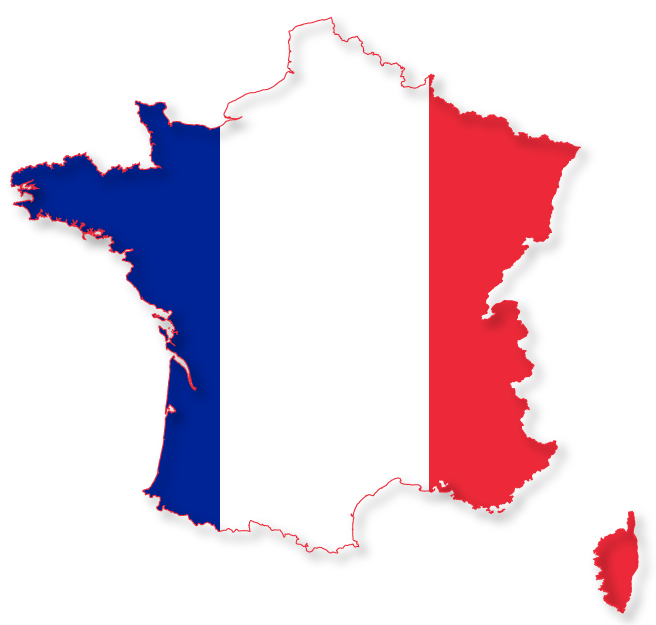
\includegraphics[height=2em]{img/france.png}}}{}}
%\addcontentsline{toc}{section}{\texorpdfstring{\protect\raisebox{-0.5ex}{\protect\makebox[3ex]{\protect
\includegraphics[height=1em]{img/flag-france.png}}}}{} in French}
%%% =============================================================
%%\index{Summary!en français}
%%\index{Summary!en français \protect\makebox[3ex]{\protect
\includegraphics[height=1em]{img/flag-france.png}}}
%\index{Summary!Résumé \protect\makebox[3ex]{\protect
\includegraphics[height=1em]{img/flag-france.png}}}
%
%Pour vous simplifier beaucoup de tâches longues et ardues, vous avez
%certainement déjà utilisé un ordinateur et en étiez très satisfaits.
%% 
%Cependant, de temps à autre, l'ordinateur ne fait pas ce que vous lui
%demandez: vous cliquez sur le bouton ``Faire ça'' et il ne le fait
%pas. Ou pire, l'ordinateur se bloque et ne répond plus à aucune
%commande. D'importantes heures de travail viennent peut-être de
%s'envoler.
%% 
%Vous gardez votre sang-froid, redémarrer l'ordinateur et tout semble à
%nouveau marcher comme prévu.
%% 
%L'erreur ne vient visiblement pas de l'ordinateur lui-même, mais elle
%semble venir du \emph{logiciel} qui contrôle ce dernier.
%% 
%Vous vous demandez pourquoi cette erreur n'a pas été corrigée, et qui
%plus est, pourquoi on ne s'est pas \emph{assuré} dès le départ que
%l'erreur ne survient pas. %survient
%
%Les différentes composantes électriques de la machine peuvent tomber
%en panne. Historiquement, ces erreurs sont appelées des \emph{bugs} %
%-- le terme anglais pour cafards -- %,
%car il est dit qu'un vrai cafard est entré un soir dans le châssis
%d'une machine qu'un informaticien fabriquait dans son garage,
%détruisant au passage quelques morceaux du circuit électrique. En se
%réveillant le lendemain, il s'est rendu compte que la machine
%manifestait un comportement bizarre.  Le terme est resté et est
%maintenant utilisé pour qualifier toutes sortes d'erreurs de
%programmation en général.
%% , c'est-à-dire quand un programme ne
%% solutionne pas le problème donné.
%
%Étant donné la complexité des ordinateurs de nos jours, il n'est pas
%étonnant qu'ils soient sujets à de nombreuses erreurs.
%% 
%Ils nécessitent de prendre en charge une multitude de
%paramètres, %et de caractéristiques,
%sans oublier les erreurs humaines introduites lors de la phase de
%programmation.
%% 
%C'est pourquoi %il est préférable
%la tendance est %
%de construire ces machines en composant plusieurs unités plus
%réduites.
%% 
%Chaque unité est de ce fait plus facile à contrôler, mais
%ces unités peuvent communiquer les unes avec les autres à n'importe
%quel moment.
%% 
%Il devient alors très difficile de prendre en compte tous les
%scénarios possibles et de prédire le comportement général du
%programme, à cause de ce caractère imprévisible. % hasardeux
%
%Les entreprises fabriquant ces logiciels n'ont pas intérêt à y laisser
%des bugs, puisqu'une erreur %quelque part
%peut engendrer d'autres erreurs en cascade.
%% 
%Celles-ci passent du temps, et de l'argent, à traquer ces bugs et s'il
%y en a trop, il n'est simplement plus rentable ou même envisageable de
%les éliminer.
%% 
%Les entreprises mettent donc en place, dans le cycle de développement de
%chaque projet, une phase essentielle de contrôle de qualité.
%% 
%Cela dit, certains bugs sont plus urgents à résoudre que d'autres.
%% 
%Ce n'est pas très grave si on ne peut pas décrocher son téléphone lors
%d'un appel, ou si l'éditeur de texte perd les derniers ajouts à notre
%document. C'est peut-être très ennuyeux mais le pronostic vital n'est
%pas engagé! On s'en remettra, en attendant la mise à jour du logiciel
%incriminé.
%% 
%Par contre, ce n
%'est pas le cas pour ces systèmes, dits
%\emph{critiques}, pour lesquels la sûreté est primordiale. Toutes les
%erreurs doivent être éliminées, qu'elles soient au niveau logiciel ou
%au niveau de la machine.
%% 
%Il n'est pas acceptable, par exemple, qu'un pacemaker s'arrête de
%fonctionner quand on passe le portique dans le métro, que l'avion
%parte en chute libre quand l'équipage allume le signal d'interdiction
%de fumer à bord, ou encore que deux trains entrent en collision parce
%que les feux ont mal fonctionné.
%% 
%% C'est pourquoi 
%Il est nécessaire de concevoir des techniques pour détecter ce genre
%d'erreurs.
%
%Pour améliorer la qualité des logiciels, il existe une technique
%prédominante: la méthode qui vise à soumettre le programme à une série
%de \emph{tests} et d'en observer les résultats.
%% 
%Ces scénarios de tests sont soigneusement conçus afin de couvrir un
%maximum d'exécution possible du programme.
%% 
%Dans la même catégorie, il est possible d'extraire un \emph{modèle} du
%programme %
%% , en prenant soin d'éliminer les morceaux superflus pour les
%% tests en cours, et 
%et de l'utiliser pour \emph{simuler} le programme.
%% 
%Cela dit, lorsque le programme est de plus en plus grand et complexe,
%que l'on utilise un modèle ou le programme lui-même, il devient
%impossible de \emph{garantir} que toutes les exécutions soient prises
%en compte par une batterie de scénarios.
%% 
%C'est même tout bonnement impossible lorsque le programme contient un
%paramètre qui varie sur un domaine non borné, comme par exemple, un
%entier.
%% 
%Ces deux méthodes sont utiles pour découvrir rapidement de simples
%erreurs, mais les erreurs subtiles, comme celles concernant le timing,
%restent non détectées.
%% 
%Dans le cas des systèmes qui requièrent une sûreté maxi\-male, il
%n'est pas concevable d'utiliser un programme qui pourrait contenir une
%erreur, quand bien même il ait passé tous ses tests.
%
%Comment donc s'assurer que toutes les exécutions d'un programme aient
%été prises en compte?
%% 
%On ne peut certainement pas faire tourner le programme et se contenter
%d'un ensemble restreint d'exécutions ou de valeurs pour les paramètres
%du programme.
%% 
%La technique d'\emph{analyse statique} offre une couverture complète
%d'un programme, sans l'exécuter. Elle inspecte toutes les exécutions
%\emph{faisables}, c'est-à-dire celles que le programme \emph{peut}
%effectuer et non celles qu'il \emph{va} effectuer.
%% 
%Le code source du programme y est sous la loupe, qu'il soit lisible
%par un humain ou seulement par une machine.
%% 
%Chaque combinaison est prise en compte ce qui rend cette méthode
%rapidement ingérable.
%% On pourrait être moins naïf, et se limiter à
%% certaines parties du code qui peuvent contenir les erreurs. Cependant,
%% déterminer leur emplacement est certainement aussi difficile que de
%% chercher les erreurs elles-même.
%% 
%% Il nous faut une autre méthode. %
%Cette thèse se concentre autour du problème suivant: %
%concevoir une méthode qui \emph{garantisse} qu'aucune erreur ne reste
%inaperçue, tout en restant dans des proportions raisonables.
%
%%% ------------------------
%Pour pouvoir vérifier qu'un programme soit correct, il s'agit d'abord
%de définir ce à quoi il doit se conformer ---appelé formellement sa
%\emph{spécification}.
%% 
%En listant l'ensemble des configurations à éviter, en listant tous les
%comportements souhaitables (ou une combinaison des deux), on décrit
%les propriétés que le programme doit satisfaire.
%% 
%Il en existe deux catégories: les propriétés de \emph{sûreté} et les
%propriétés de \emph{vivacité} (Safety et Liveness en anglais).
%% 
%Par exemple, ``le pacemaker ne s'arrête jamais'', ``l'airbag ne doit
%pas prendre plus de $x$~millisecondes pour s'ouvrir'', ou encore
%``aucun processus ne peut bloquer tous les autres'' sont des
%propriétés de sûreté. On doit s'assurer que le programme ne soit
%jamais dans une mauvaise configuration.
%% 
%À l'inverse, ``le facteur livre le courrier à son destinataire'', ``le
%système ne stagne pas'' ou encore ``le serveur prend en charge une
%requête internet'' sont des propriétés de vivacité, où l'on
%s'intéresse aux bonnes configurations du programme, associées à
%certaines probabilités.
%% 
%C'est à nous de définir ce que la spécification doit inclure, pour
%s'accorder avec la vérification souhaitée.
%% 
%Un système d'anti-blocage de freins (ABS), par exemple, calcule le
%freinage adéquate. Toutefois, si ce calcul ne se fait pas dans le
%temps imparti, le système n'est pas considéré comme un comportement
%désirable, et est donc défectueux.
%% 
%Dans cette thèse, nous nous concentrons sur les propriétés de sûreté.
%\begin{statement}
%  {\bf Sûreté}: %
%  {\it Étant donnée une spécification, le système peut-il se retrouver\\dans une mauvaise configuration?}
%\end{statement}
%
%%% ------------------------
%Plutôt que de tester le programme dans des scénarios particuliers, ou
%d'en analyser le code source, on utilise un cadre mathématique, dit de
%\emph{vérification formelle}, qui permette de \emph{prouver} qu'un
%programme soit conforme à sa spécification.
%% 
%Plus particulièrement, on cherche à prouver l'absence d'erreur, de
%manière \emph{automatique}, c'est-à-dire sans intervention de
%l'utilisateur.
%% 
%On commence par extraire un modèle qui corresponde aux comportements
%du programme origi\-nel, tout en en éliminant les parties sans
%rapport %importance
%au vu de la propriété à vérifier.
%% 
%Toutefois, comment faire lorsque le programme manipule des entités non
%bornées? On parle alors de système à états infinis et on en construit
%une approximation qui respecte malgré tout l'essence même du programme.
%
%De nombreux systèmes à états infinis peuvent en fait être caractérisés
%par une famille de systèmes à états finis, avec un paramètre (ou plus)
%variant dans un domaine non borné.
%% 
%Pour chaque valeur du paramètre, le système est à états finis.
%% 
%Le paramètre peut par exemple être 
%% la taille d'une base de données,
%le nombre de processus associés à une session donnée d'un protocole, %
%le nombre de n\oe{}uds dans les mailles d'un réseau, %
%ou encore l'agencement des différentes composantes d'un programme (et
%implicitement comment elles communiquent entre elles).
%% 
%Les systèmes qui contiennent un paramètre \emph{a priori} inconnu
%doivent se comporter correctement quelle que soit la valeur du
%paramètre. Ils sont ainsi considérés comme des systèmes à états
%infinis, et on les appelle des systèmes paramétrés.
%%
%%% ---------------------------
%Dans cette thèse, nous présentons deux méthodes pour vérifier certaines
%propriétés de sûreté de ces systèmes paramétrés.
% 
%La première méthode fait machine arrière: elle part des états erronés
%du système en général, et calcule à quoi ressembleraient les états du
%système qui pourraient mener à une erreur.
%% 
%Autrement dit, elle trouve l'ensemble des configurations qui sont
%directement et indirectement mauvaises.
%% 
%Si les états initiaux du système originel ne font pas partie de cet
%ensemble, le programme peut être considéré comme correct. Il faut bien
%sûr d'abord s'assurer que l'approximation du modèle extraite du
%programme de départ corresponde à ce dernier.
%
%La deuxième méthode démarre des états initiaux. Elle se limite à de
%petites valeurs du paramètre, et en déduit un seuil pour lequel il
%n'est pas nécessaire de continuer les calculs: la méthode a en effet
%toutes les données nécessaires pour conclure qu'il n'existe pas de
%mauvaises configurations pour les valeurs du paramètre plus grandes
%que ce seuil.
%% 
%En simplifiant, la méthode décompose chaque configuration en petits
%morceaux d'une certaine taille, et se charge de recombiner ces
%morceaux de toutes les manières possibles, en particulier en
%configurations de toutes tailles (un peu comme des briques de Lego).
%%
%L'idée est de collecter tous les petits morceaux, et de s'assurer
%qu'aucune des recombinaisons ne correspond à une mauvaise
%configuration.
%%
%Si c'est le cas, le seuil est trouvé. Si ce n'est pas le cas, on
%recommence avec des morceaux de taille un peu plus grande.
%
%En dernier lieu, il est intéressant de se demander dans quelles
%conditions la méthode termine. Le problème est classé dans la catégorie
%des problèmes indécidables, c'est-à-dire qu'il n'y a pas de méthode
%générale pour solutionner \emph{toutes} les instances du
%problème. Cela dit, pour certaines instances, ces deux méthodes
%s'avèrent être efficaces et peuvent même parfois être garanties de
%terminer.
%% 
%En effet, alors que d'autres méthodes prenaient des heures, ces
%méthodes permettent de vérifier certains programmes en quelques
%secondes, ce qui %Ces temps de calculs raisonnables étaient
%était le but recherché.
%%
%Cette thèse démontre notamment l'efficacité de ces méthodes en
%s'attaquant au problème complèxe d'analyse de formes, c'est-à-dire aux
%programmes concurrents manipulant des listes liées. %en mémoire.
%% \qed


\begingroup
\clearpage
% To adjust the indentation in your table of contents, uncomment and enter the widest numbers for each level
%  E.g.  \settocnumwidth{widest chapter number}{widest section number}{widest subsection number}...{...}
%  \settocnumwidth{5}{4}{5}{3}{3}{3}
%\initializepartialtoc
\tableofcontents
%\adjusttocfornonnumberedchapters % Adjusting the small ToC counters
\endgroup

%% Optional tables
%\listoftables
%\listoffigures

\chapter{How to read this thesis}
This document is a comprehensive summary.
\index{Thesis outline}

%\paragraph{Outline.}
\bigskip%
%
We first describe the domain of formal verification, where this thesis
belongs, and approach the problem in a top down fashion.

%
We present two techniques in
Chapter~\ref{chapter:monotonic:abstraction}~and~\ref{chapter:view:abstraction}
to prove safety properties for a wide range of programs (listed in
Chapter~\ref{chapter:case:studies}).
%
Finally, we dedicate Chapter~\ref{chapter:shape:analysis} to the
problem of shape analysis. It deals with a class of programs that
manipulate memory heaps concurrently.
%
To finish, we give some conclusions and potential directions for
future research topics.


\addtocontents{toc}{\protect\hrulefill}

%% -------------------------------------
 
%% -------------------------------------
\mainmatter
%% -------------------------------------
%% ====================================================================
\chapterwithtoc{Introduction}
\label{chapter:verification}
%% ====================================================================

Computers have been used for variety of applications in business, science, education, engineering and so on. They help to solve real world problems that would otherwise be slow, impossible or extremely difficult to address without computers and software. However, sometimes they do not behave exactly as we expect them to do. \bjcom{skip ``do''}
In some cases, the consequence could be very serious for errors in banking systems
and flight control systems.
\bjfix{In some cases, the consequence could be very serious for errors in banking systems and flight control systems.}
{In many cases, the consequences could be very serious, for example when errors
in banking or flight control software results in unexpected behaviors.}
Errors in computer systems are mostly not caused by the machine itself, but typically originate from the software that controls the computer systems, so called bugs. 
%% ********************************************************************
\KW{Complex machines}%
%% ********************************************************************
Bugs are quite common  in complex software systems,
since they typically have complicated input and involve many features which makes them difficult to design and make them perfect by human effort.
\bjfix{Bugs are quite common  in complex software systems,
since they typically have complicated input and involve many features which makes them difficult to design and make them perfect by human effort.}
{Bugs are quite common  in complex software systems,
since they typically have complicated input and involve many features which makes them difficult to design and make them perfect by human effort.}
%% ********************************************************************
\KW{Find bugs}%
%% ********************************************************************
Detecting and fixing software bugs are important tasks in software development process. Remaining undetected bugs in any software project may lead huge
problems. They can be very hard to detect and correct. It will
become too costly to solve. Therefore, it is very important to allocate sufficient
resources, both in terms of time and manpower, to ensuring that developed
software is as free of bugs as possible.

%% ********************************************************************
\KW{Safety$\Rightarrow$no bugs}%
\index{Critical systems}%
\index{Safety}%
%% ********************************************************************

Some bugs are less serious than others. In some cases, we can still use software programs with these bugs. For example, bugs appearing in computer games and online news. However, in the case of critical systems 
%such as banking, software systems in airplanes, safety is the most important aspect and we have to ensure that there no bugs in either the software nor the hardware.
especially algorithms in libraries of programming languages, safety is the most important aspect and we have to ensure that there no bugs. These algorithms are used in many applications, and bugs will have wide impacts. Some of such libraries provide standard data structures such as stacks, queues, containers. These data structures provide ways of storing multiple values in a single variable. It is used to organize data in such a way that the insertion deletion,searhing i.e manipulation of data is done with minimal complexity , and that gives a efficient performance of our computing. By using data structures data can be easily, and efficiently exchanged; it allows portability, comprehensibility, and adaptability of information.

A data structure is a particular way of organizing and storing data in a computer so that it can be accessed and modified efficiently. More precisely, a data structure is a collection of data values, the relationships among them, and operations that can be applied to the data. 
%Each data structure has it own specification which describes the behaviour of the data structure. 
A data structure can be both sequential or concurrent, concurrent data structures can be accessed and manipulated concurrently by many parallel threads are a central component of many parallel software applications. 
%They should allow a large degree of parallelism among accessing threads to minimize serialization bottlenecks, while maintaining the appearance of atomic operations. 
Data structures typically use heap-allocated memory to store their data. For example, concurrent link queue in java.util.concurrent uses singly linked list data structure to store data.   


%Many modern programming languages provide libraries of concurrent data structures (e.g., the java.util.concurrent package and Intel Threading Building Blocks library) that are widely used. 



The predominant method to improve software quality is
\emph{testing}. It is a dynamic analysis where a program is run under specific conditions, so-called test cases, and checking
whether the result with a given input matches the expected output.
%
The test cases are carefully designed to cover all possible cases of program executions.\index{Coverage}
%% ********************************************************************
\KW{Simulation}\index{Verification Methods!Simulation}%
%% ********************************************************************
%Similarly, we can check for correctness of a program by using a \emph{model} of the program. The model can be extracted by
%removing all parts that are irrelevant for the tests, and can be used
%to \emph{simulate} the executions. 
However, there is no guarantee to cover all possible executions. Therefore, we have to find the way to achieve a full coverage of program executions. \emph{testing} can be used to show the presence of bugs, but never to show their absence. So, it is needed to use formal verification that a software system is correct with respect to some specifications. %
%
% The topic of this thesis is centered around the following question.
% %
% \begin{statement}
%   \it%
%   Can we design a method that would give us\\%
%   \emph{guarantees} that no error is left undetected\\%
%   and that does not (too much) suffer from state-space explosion?
% \end{statement}

%\index{Error-free Guarantee}%
%The topic of this thesis is design methods guaranteeing that no error is undetected and that do not suffer from state-space explosion.

%% ====================================================================
\section*{Formal Verification} 
%Computer programs are written based on human intuition, which is probably leads to programming errors. Current practice is to test programs on various sample inputs in the hope of finding any possibility of incorrect program behavior. There exist many approaches like testing, simulation, static analysis and simple debugging techniques, such as inserting assertions and print statements in the source code, which show the presence of software errors. 

%Formal verification uses mathematical methods to verify whether a software satisfies its specification provided by users. 
%formal verification is the process of checking whether a software satisfies its predefined properties. 
Formal verification uses mathematical methods to check whether a software satisfies its specification provided by users. 
%formal verification is the process of checking whether a software satisfies its predefined properties. 
%\bjcom{Skip the following sentece. Continue into the next paragraph}
%There is a wide variety of specification to be checked for software programs, these specification can be very domain-specific, as in “train collisions and derailments do not occur in train traffic” or it may be generic, as in “no execution of the system dereferences a null pointer.” 
% be either safety or liveness properties. Liveness properties state that program execution eventually reaches several desirable states at some point of execution, for example liveness properties can be "the postman delivers the letter to the recipient", "A sent message is eventually received". In contract, verifying safety property of a program is satisfied is reduced to checking that something bad will never happen in the execution of the program [48]. 
%\input model
%In order to specify liveness properties, it is needed to  describe traces of events by using temporal logics, statistics, and probabilities. Checking aliveness property is done by repeatedly checking reachability of good situations in program executions. 
There are several approaches for formal verification, including equivalence checking, theorem proving, and model checking. Equivalence checking method decides whether a system is equivalent to its specification with respect to some notion of behavioral equivalence. This is \bjcom{Insert a sentence about where it is used. I think it is mostly used for hardware designs in industry} Theorem proving is a technique where both the \bjcom{insert ``behavior of the''} system and its desired properties are expressed in mathematicaal logic. Then, theorem proving \bjcom{insert ``typically assisted by an interactive theorem prover} will try to prove that the system satisfies these properties. 

Model checking approach take \bjfix{Model checking approach take}{Model checking takes as input} a model of the system under
consideration and a formal specification of the \bjfix{the}{a} property to be verified as inputs. \bjcom{Insert a sentence saying like ``The specification of a software component may consist of a number of such properties, each of which can be verified using model checking''}
The approach exhaustively explorer \bjcor{explores} all possible states  \bjcor{executions} of the model \bjcom{En the sentence here, and start a new one with ``This is typically done exploring the set of reachable states of the model''}  which can be finite or infinite \bjcom{Stop the sentence here, the stuff about infinite and abstraction comes later. Instead, start here by saying that this works well if the set of reachable states is finite, and also say in which application domains this has been successful} where infinite sets of states can be represented finitely by using abstraction techniques. In this way, it can be shown that a given system model truly satisfies a certain specification. Model checking is a general verification approach that is applicable to a wide range of applications
  such as embedded systems, software engineering, \bjcom{Skip ``software engineering''} and hardware design. However, it usually work well with finite-state systems. It is a real challenge to examine the largest possible state spaces that can be treated. For example, applying model checking to infinite-state systems such as data structures with many dimensions of infiniteness is a real challenge in current software verification research.
  \bjcom{The preceding paragraph needs better structure. You can use the flow: what is model checking - it works well for finite-state, e.g., for controllers and hardware design - most software is infinite-state, e.g., a data structure may contain an unbounded amount of data - a common technique for handling this is to devise a symbolic representation of sets of states, such that a single symbolic representation may represent an infinite set of states. Thereafter you can give an overview of
  what has been achieved using symbolic techniques}
%In this thesis though, we consider programs where the specification describes the bad behaviors. We concentrate on safety properties and try to design abstraction techniques to verify that a program including both sequential and concurrent program respects its specifications. 

%\section*{Verification of Data Structures}
%Most modern programming languages provide libraries of data structures such as the C++ Standard Template Library, the Java Collections Framework. A data structure is a particular way of organizing and storing data in a computer so that it can be accessed and modified efficiently. More precisely, a data structure is a collection of data values, the relationships among them, and operations that can be applied to the data. Each data structure has it own specification which describes the behaviour of the data structure. A data structure can be both sequential or concurrent, concurrent data structures can be accessed and manipulated concurrently by many parallel threads are a central component of many parallel software applications. They should allow a large degree of parallelism among accessing threads to minimize serialization bottlenecks, while maintaining the appearance of atomic operations. Many modern programming languages provide libraries of concurrent data structures (e.g., the java.util.concurrent package and Intel Threading Building Blocks library) that are widely used. 
%
%To ensure that a concurrent data structure is correct, we have to ensure that it respects to its sequential specification.  Ideally, the correctness is captured by linearizability. Linearizability is generally accepted as the standard correctness criterion for such concurrent data structure implementations. It states that each operation on the concurrent data structure can be viewed as being performed atomically at some point (called linearization point (LP)) between its invocation and return. The linearizability guarantee relieves the programmer from complex reasoning about possible interference among data-structure methods and removes the need to add explicit synchronization. Concurrent implementations of abstract data structures (stacks, queues, sets, etc.) are becoming more and more complex as implementations that increase the degree of concurrency are identified. This in turn is making linearizability verification harder. Existing approaches lack generality as they are limited to specific classes of concurrent data structures so far no technique (manual or automatic) for proving linearizability has been proposed that is both sound and generic. In this thesis, we focus on verifying safety properties including linearizability of both sequential and concurrent data structures.
\section*{Research Challenges}
%In this thesis, we consider two challenges in software verification, the first challenge is to automate its application to sequential programs that manipulate complex dynamic linked data structures. The problem becomes even more challenging when program correctness depends on relationships between data values that are stored in the dynamically allocated structures. Such ordering relations on data are central for the operation of many data structures such as search trees, priority queues (based, e.g., on skip lists), key-value stores, or for the correctness of programs that perform sorting and searching, etc. The challenge for automated verification of such programs is to handle both 
%\begin{challenges}
%\item infinite sets of reachable heap configurations and
%\item relationships between data values embedded in such graphs, 	
%\end{challenges}
%e.g., to establish sortedness properties, there exist many automated verification techniques, based on different kinds of logics, automata, graphs, or grammars, that handle these pointer structures. Most of these approaches abstract from properties of data stored in dynamically allocated memory cells. The few approaches that can automatically reason about data properties are often limited to specific classes of structures, mostly singly-linked lists (SLLs), and/or are not fully
%automated.
%
%We present a general framework for verifying programs with complex dynamic linked data structures whose correctness depends on relations between the stored data values. Our framework is based on the notion of forest automata (FA) which has previously been developed for representing sets of reachable configurations of programs
%with complex dynamic linked data structures [?]
\bjcom{Start by saying what is the overall challenge of your thesis. Then say that this requires to address several challenges in model checking}
In this thesis, we consider challenges in developing techniques for automated verification of both sequential and concurrent data structures using heaps. 
%Our challenges are to automate its application to both sequential and concurrent programs that manipulate complex dynamic linked data structures. We have to deal with concurrent programs with an unbounded number of threads that concurrently access and manipulate a dynamically allocated shared heap where data stored in each heap cell can be in unbound domain. Such programs and algorithms are difficult to get correct and verify, since their shapes are complicated to represent and they typically employ fine-grained synchronization, replacing locks by atomic operations such as compare-and-swap, and are therefore notoriously difficult to get correct, witnessed. It is therefore important to develop efficient techniques for automatically verifying their correctness. This requires overcoming several challenges. This thesis presents simple and efficient techniques to verify that a concurrent implementation of a common data type abstraction, namely queue, stack, set, conforms to a simple abstract specification of its (sequential) functionality. The data structures we consider for these programs can be singly-linked lists, sets of linked lists or skip-lists. In order to deal with this problem, we have to deal with several combined challenges as follow.
We have to deal with several sub-challenges as following: 
\bjcom{I suggest to use more standard bullets. Each bullet can have a number of letter, and have a heading of a few words, e.g, {\bf Dynamically heap-allocated memoty}. Also, do not just break the page here}
\bjcom{Each challenge should be described better. You must be more precise in what cannot be done with current techniques, and (on an abstract level) what you
  will try to achieve}
\newpage
\begin{challenges}
\item Heaps which are used by data structures are dynamically heap allocated memory. Therefore, we have to deal with unbounded number of heap cells. In this thesis, we propose three heap abstraction techniques to address the challenge, including forest automata, summary abstraction and view abstraction.
\item In each cell of a heap, the domain of data values can be unbounded. We use the combination of shape analysis and data abstraction to deal with this challenge. 
  \bjcom{I suggest to start with this challenge (since it is the first paper). You can start the preceding text and simplify it. The important aspect is that there
    are current approachs for heaps and for data, but not for combining them in suitable ways, and thereafter you describe very briefly your approach. Here is
    the disappeared text: ``In this thesis, we consider two challenges in software verification, the first challenge is to automate its application to sequential programs that manipulate complex dynamic linked data structures. The problem becomes even more challenging when program correctness depends on relationships between data values that are stored in the dynamically allocated structures. Such ordering relations on data are central for the operation of many data structures such as search trees, priority queues (based, e.g., on skip lists), key-value stores, or for the correctness of programs that perform sorting and searching, etc. The challenge for automated verification of such programs is to handle both 
\begin{itemize}
\item infinite sets of reachable heap configurations and
\item relationships between data values embedded in such graphs, 	
\end{itemize}
e.g., to establish sortedness properties, there exist many automated verification techniques, based on different kinds of logics, automata, graphs, or grammars, that handle these pointer structures. Most of these approaches abstract from properties of data stored in dynamically allocated memory cells. The few approaches that can automatically reason about data properties are often limited to specific classes of structures, mostly singly-linked lists (SLLs), and/or are not fully
automated''}

We present a general framework for verifying programs with complex dynamic linked data structures whose correctness depends on relations between the stored data values. Our framework is based on the notion of forest automata (FA) which has previously been developed for representing sets of reachable configurations of programs
with complex dynamic linked data structures [?]

\item We have to verify that the data structures are correct with any number of threads that access and manipulate the structures. We use the thread modular technique to dead with this challenge.
\item \bjcom{This paragraph should be improved. I suggest to make it the second challenge. You can start by saying that for concurrent data structures, you address
  a number of challenges, and then you have three bullets for each of them. The first is how to specify correctness in a way that is suitable for automated verification, the second is how to deal with an unbounded number of threads, the third is to provide a simple shape abstraction which can express relevant properties of different classes of heap structures: You can talk about skiplists, and their challenges}
To ensure that a concurrent data structure is correct, we have to ensure that it respects to its sequential specification.  Ideally, the correctness is captured by linearizability. Linearizability is generally accepted as the standard correctness criterion for such concurrent data structure implementations. It states that each operation on the concurrent data structure can be viewed as being performed atomically at some point (called linearization point (LP)) between its invocation and return. The linearizability guarantee relieves the programmer from complex reasoning about possible interference among data-structure methods and removes the need to add explicit synchronization. Concurrent implementations of abstract data structures (stacks, queues, sets, etc.) are becoming more and more complex as implementations that increase the degree of concurrency are identified. This in turn is making linearizability verification harder. Existing approaches lack generality as they are limited to specific classes of concurrent data structures so far no technique (manual or automatic) for proving linearizability has been proposed that is both sound and generic. In this thesis we provide a sound and generic technique to verify linearizabilities of concurrent data structures.
\item In some data structures, the each cell can have unbound number of pointer field such as cells in skip-lists and arrays of lists. This problem is solved by our fragment abstraction technique.
\end{challenges}

\bjcom{The outline must be more complete.}
We present, in the next chapters, the general background about model checking, concurrent data structures. Thereafter, in the following chapter, we introduce in a stepwise manner how
we cope with  above challenges. In the last chapter, we summary and give future plans for our work.

%% ====================================================================
\chapter{Model Checking}
\label{section:model:checking}
\index{Model Checking}%
\index{Verification Methods!Model Checking}%
%% ====================================================================
%
% Within the field of formal verification, 
The approach that we focus on this thesis is
\emph{model-checking}.
%% ********************************************************************
\KW{Automation}%
\index{Automation}%
%% ********************************************************************
This method will try to verify whether a model of the program
satisfies its specification.
%
%It is often called a push-button technology.
%
 
This approach was introduced by Emerson and Clarke~\cite{CE82} and by Queille and Sifakis~\cite{QS82}. The method requires a model of the system under
consideration and a property as input. The method then computes and returns either "correct" when the specification is satisfied by the program, or "incorrect" when the program does not satisfy its specification. In the case of incorrect answer, the method can explain the reason by giving a counter-example. A state in the model contains relevant information about the program. Alongside all the states of the system, the model depicts the
transitions, i.e.\ how to move from one state to another state. Every behaviour of the system is represented as a succession of transitions, starting from some initial states. States and transitions together describe the \emph{operational
  semantics}, that is, how every step of the system takes place in the model. The number of states and transitions can be finite or infinite. Model-checking aims to explore the state-space entirely from some initial states. However, when the state-space is of large size. It grows in-fact
exponentially with the number of parameters or the size of their
domain. Therefore, there have been several methods to address with the
state-space explosion problem.
%\begin{figure}[h]
%{\noindent\centering %
%  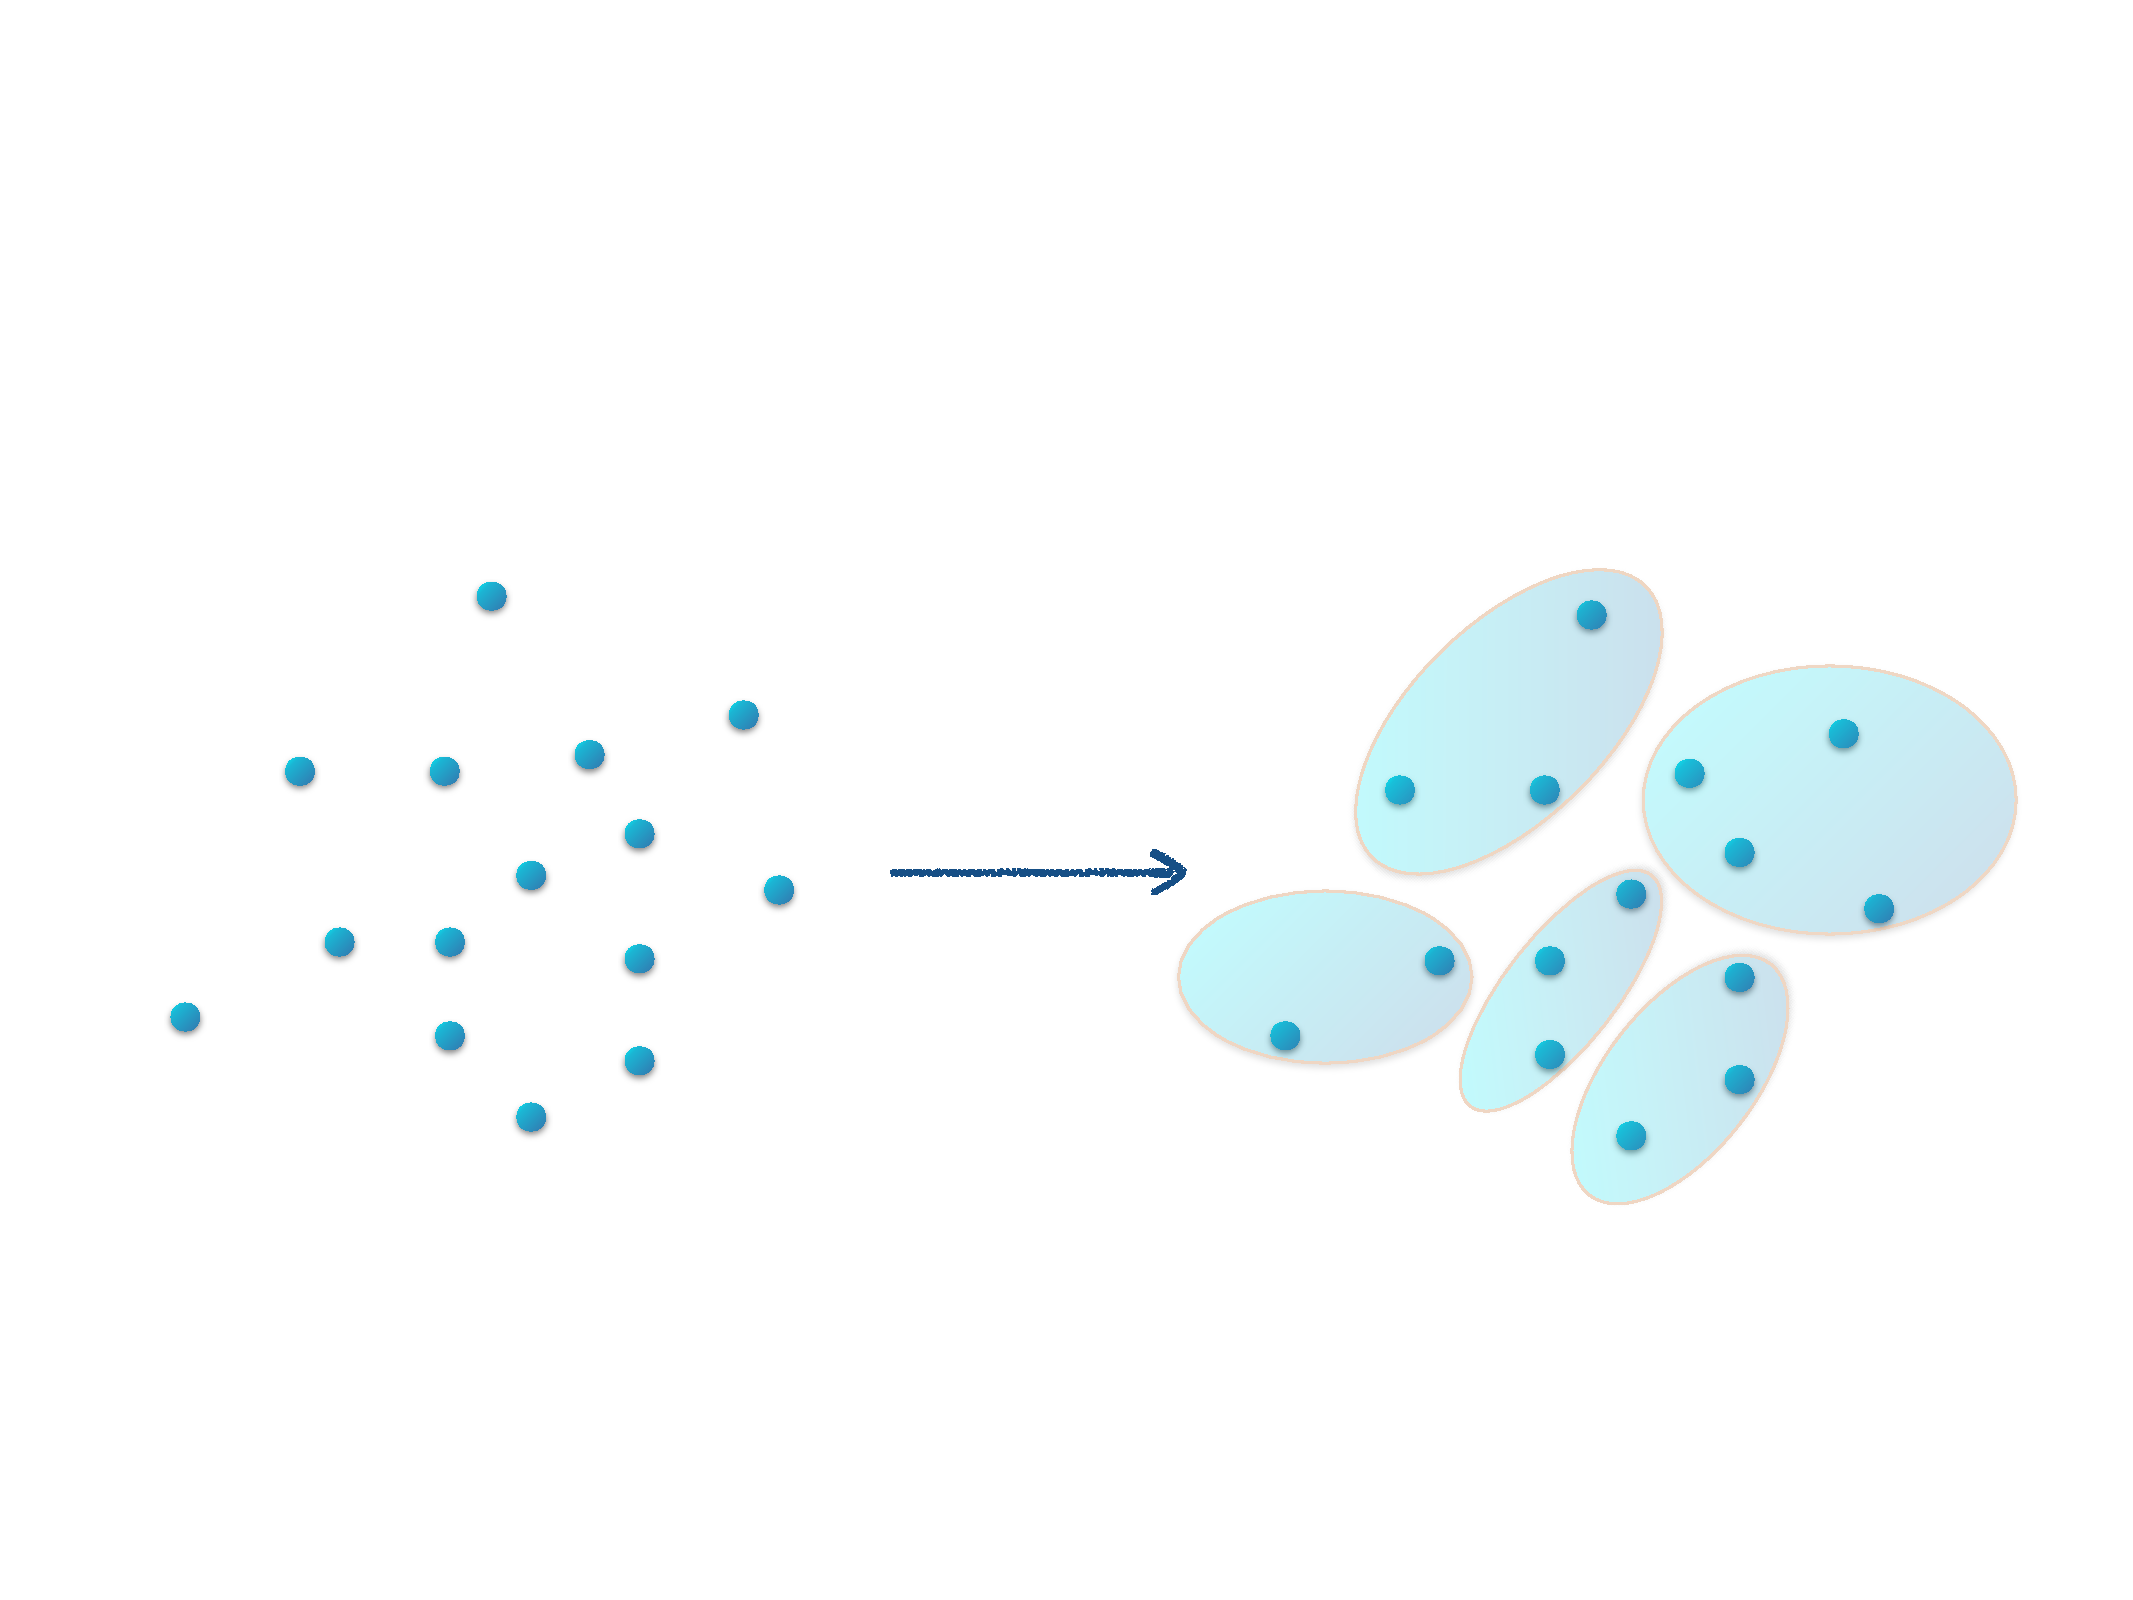
\includegraphics[trim=4cm 4cm 1.5cm 2cm,clip,scale = 0.3]{img/modelchecking.pdf}%
%  \par%
%}%
%\caption{Example of symbolic representation where the right part is a concrete reachable state-space and the left part is abstract state-space using symbolic representation}
%\label{symbolicabs}
%\end{figure}
%\vspace{1cm}
%\begin{figure}[h]
%  \centering
%  \tikzinput{img/symbolic-representations}    
%  \vspace{0.3cm}
%  \caption{Symbolic Representation}      
%\label{symbolicabs}
%\end{figure}
%\vspace{1cm}
                   
There are several techniques addressing the state-space explosion problem.
The choice of which transition to pick during the exploration can be
crucial for the efficiency of the procedure. In some cases, exploring all orderings of events is not necessary because some states can be re-visited. \emph{Partial order} techniques aim at detecting and avoiding
redundant situations, while retaining important dependencies among
actions. They however do not reduce the state-space. The main approach called \emph{symbolic
  representation}  to solve the state-space explosion problem is to avoid representing concretely all states of the system. The process is performed by designing abstract states so that each abstract state could represent a set of concrete states.  This designing process is done by \emph{dropping} irrelevant details based on properties that we want to verify. For example, consider a switch with two positions: {\tt up} and {\tt down}. The switch has a counter that indicates how many times the light was turn on. Initially, its position is {\tt down}, the light is {\tt off} and the counter is $\tt 0$. When the switch is shifted up, the light is turned on, and the counter is incremented by $\tt 1$. When we shift the switch down, the light is turned off and the counter is reset to $\tt 0$ if it had reached its maximum value. We want to verify that the switch can not be up and the light is off at the same time. If we keep all the information of the system, then, a state consists of the position of the switch, the status of the light and the value of the counter, we would have $\tt (2*2*n)$ states where $\tt n$ is the maximum value of counter. If $\tt n$ is $\tt 1000000$ then we may end up to four million states.  However, it is obvious that the counter is not needed to verify the property, so we could ignore it then a state contains only the position and status of the switch and the light denoted as $\tt [p,s]$ where $\tt p$ is the position and $\tt s$ is the state of the light. The system using the symbolic representation moves from  [{\tt down;off}]  to  [{\tt up;on}]  and conversely from  [{\tt up;on}]  to  [{\tt down;off}] . We see that the state-space exploration never visits a state that belongs to the set labeled by  [{\tt down;on}]  therefore the system is safe. The switch example is of course simple and does not reflect the complexity of today’s software. Symbolic representations are of crucial help to combat the state-space explosion, accelerate the algorithms and get them to terminate in a reasonable amount of time

%By doing that, we get an set of abstract states from reachable states of a concrete system. Thereafter, the method returns safe if the abstract states do not contain any bad state. The approach described in figure \ref{symbolicmodelchecking}.  %
%
The challenge is to find over-approximations that do not introduce
behaviours that could turn out to be bad. Indeed, the method would
return that the property is not satisfied and we would not know
whether it comes from the approximation or from the concrete system
itself. % 
                                   
%\begin{figure}
%{\noindent\centering %
%  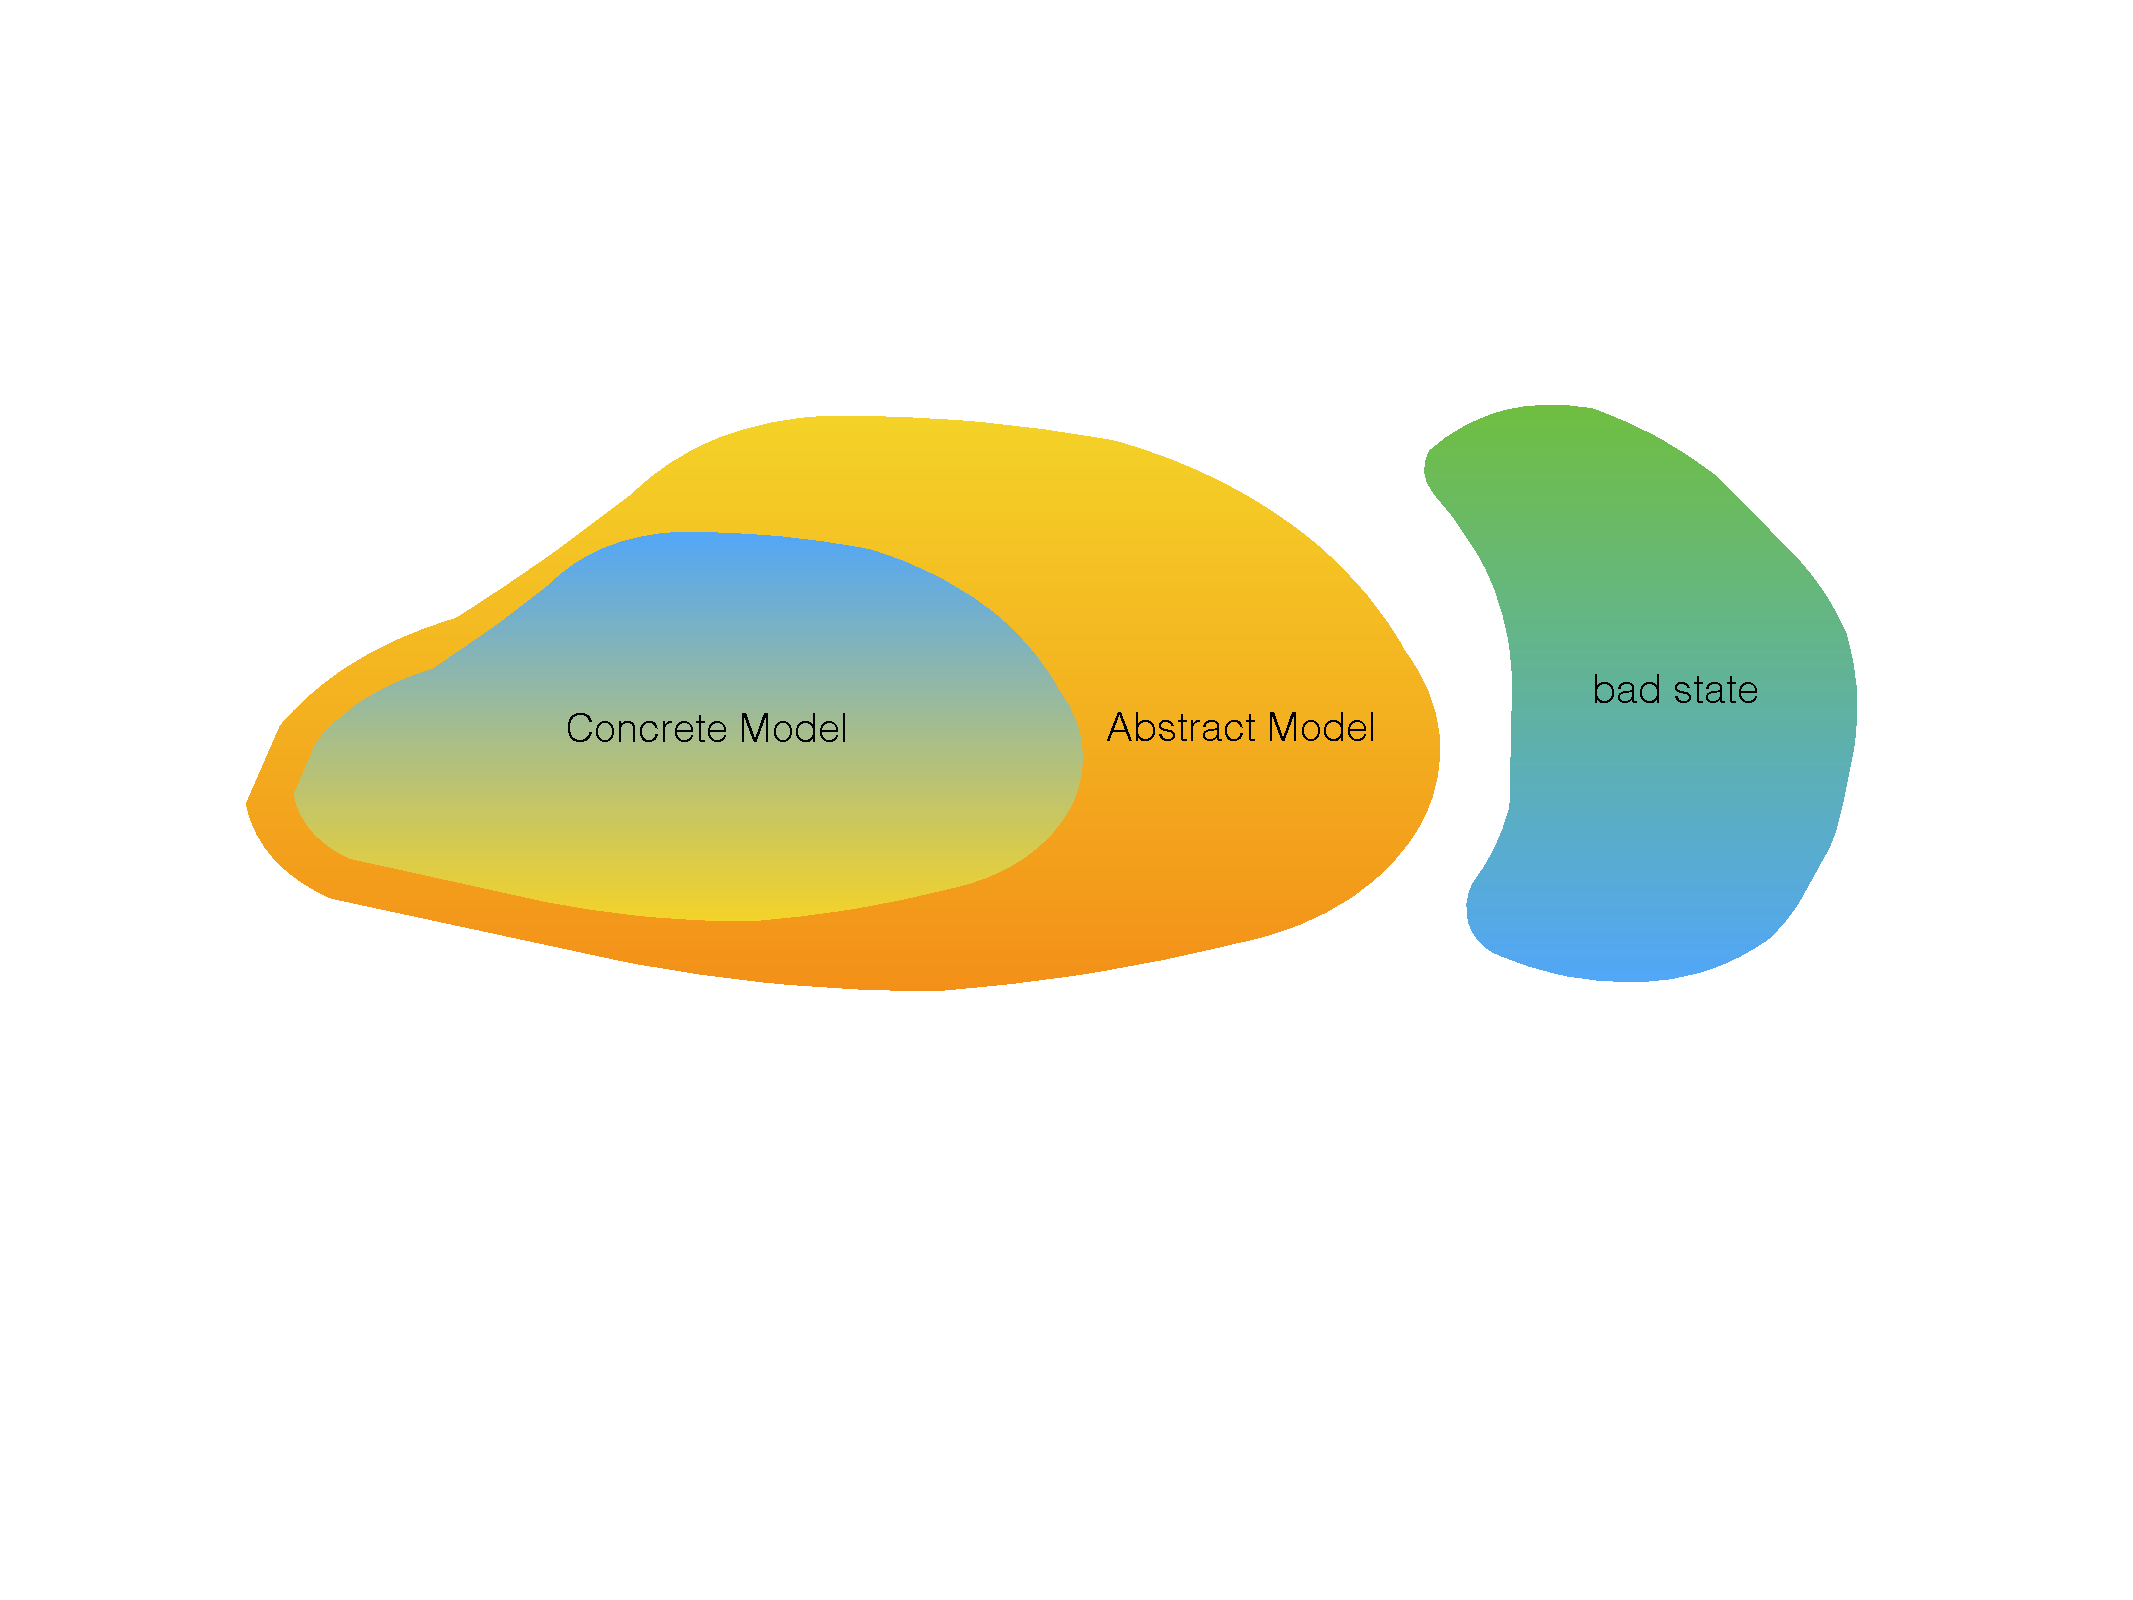
\includegraphics[trim=0cm 6cm 2cm 2cm,clip,scale = 0.25]{img/badstate.pdf}%
%  \par%
%}%
%\caption{Symbolic model checking architecture }	
%\label{symbolicmodelchecking}
%\end{figure}


%\vspace{1cm}
%\begin{figure}[h]
%  \centering
%  \tikzinput{img/approximations} 
%  \vspace{0.3cm}
%\caption{Symbolic model checking architecture }	
%\label{symbolicmodelchecking}
%\end{figure}
%\vspace{1cm}

To palliate to the imprecision caused by a too coarse
over-approximation, it is possible to analyze the returned
counter-example and find the origin of the problem. If it turns out to
be a real concrete example, the method has in fact found a bug, and
the property is surely not satisfied. Otherwise, the counter-example
comes from the approximation, that is, there is a step in the sequence
of events leading to that counter-example which is not performed by
the original system but only by the abstract model. The approximation
is be refined by discarding this step and the method should be run
anew.

Nevertheless, finding suitable over-approximations is a challenge on
its own. %
This thesis now revolves around the following problem statement.
%
%\begin{statement}
%  {\bf Safety}: %
%  {\it Given a specification and an (over-)approximation,\\does the
%    abstract system reach a bad configuration?}
%\end{statement}
%

%%%% ====================================================================
%\section{Parameterized Verification}
%\label{section:paramsys}
%%% ====================================================================
%\KW{Parameter-ized systems are infinite-state}%
%\index{Parameterized Systems}%
%%% ********************************************************************
%Many systems can actually be characterized as a family of finite-state
%systems with one (or more) parameter ranging over an unbounded domain.
%%
%For each fixed value of the parameter, the system is finite-state.
%%
%However, a system that contains an \emph{a priori} unknown parameter
%must behave properly regardless of the value of the parameter. It is
%therefore considered infinite-state.
%
%%% ********************************************************************
%\KW{Parameter-ized verification}%
%\index{Parameterized Verification}%
%%% ********************************************************************
%The \emph{parameterized verification} problem is to prove
%correctness %\footnote{\ldots and namely here safety only}
%of the system, against some specification, for all values of the
%parameter.
%%
%For example, in the case of a program manipulating a list, the
%parameter could be the length of the list. The system as a whole is a
%set of finite-state systems, one for each length of the list.
%%
%For a network protocol, the parameter could be the topology of the
%network and the system is to be proven safe regardless of how the
%network nodes are arranged.
%
%%% ********************************************************************
%\KW{Parameter-ized systems}%
%%% ********************************************************************
%We concentrate in this thesis on a specific class of
%\emph{parameterized systems}, namely, systems consisting of an
%arbitrary number of processes (see
%Chapter~\ref{chapter:parameterized:systems}). %
%The size of the system is the parameter of the verification problem.
%% 
%For each value $n$ of the parameter, the system $S_n$ is the parallel
%composition of $n$ processes, which can interact with each other at
%any time.
%%
%\index{Safety}%
%Given a specification, we prove safety for the family $(S_n)_{n\ge 0}$
%--- as~a~whole --- by showing the non-reachability of some
%(potentially infinite) set of \emph{bad states}. %
%%
%We use the following strategy:
%\begin{strategy}
%\item \index{Model}%
%  We extract a model from each process in the system. This in turn
%  defines the operational semantics with states and transitions for
%  the entire family.
%\item \index{Over-approximation}%
%  We use an over-approximation to derive an abstract model from the
%  original (infinite-state) model.  This defines a new state-space and
%  set of transitions.
%\item \index{Abstract Model}%
%  We determine two sets in the abstract model:
%  \begin{itemize}[itemsep=0pt, leftmargin=0cm]
%    % \item the initial states --- usually mirroring the initial settings
%    %   of the program,
%  \item \index{Initial states}%
%    the initial states, usually mirroring the initial settings of the
%    program,
%    % \item the bad states --- usually along the lines of the targeted
%    %   property.
%  \item \index{Bad states}%
%    the bad states, usually along the lines of the targeted property.
%  \end{itemize}
%\item \index{Reachability}%
%  We finally check whether the bad states are reachable from the
%  initial states in the abstract model.
%  % 
%  % \item Apply model-checking techniques (from
%  %   Chapter~\ref{chapter:monotonic:abstraction}~or~\ref{chapter:view:abstraction})
%  %   to determine wether the bad states are reachable from the initial
%  %   states, by following a sequence of transitions --- also known as the
%  %   reachability problem.
%\end{strategy}%
%%
%\index{Soundness}%
%By construction of the over-approximation, showing that the abstract
%model is safe, will imply that the original system is also correct
%with respect to its specification, regardless of the number of
%processes in the system.
%%
%We present a formal definition and some examples in the next chapter.
%
%%% ********************************************************************
%\newpage
%\subsection*{Heap analysis}
%\KW{Heaps}%
%\index{Heap Analysis}%
%%% ********************************************************************
%An important extension in this thesis is the application of
%parameterized verification to the complex problem of shape analysis.
%%
%We consider programs that implement data-structures that can be
%concurrently accessed by an arbitrary number of threads.
%%
%The data-structures, e.g.\ stacks and queues, are constructed using
%singly-linked lists.
%%
%By following the chains of pointers, we observe that programs leave
%memory footprints that we coin \emph{shapes} or \emph{heaps}.
%
%The number of threads is one dimension of the parametrization. 
%%
%Shape analysis can also be parameterized along other dimensions, such
%as the size of the data-structure or the data domain.
%%
%In Chapter~\ref{chapter:shape:analysis}, we address the combined
%challenges of an arbitrary number of threads, an unbounded size of
%heaps and an unbounded data domain. Moreover, we do not assume the
%presence of a garbage collector which makes the task even more
%complex.
%
%The program specification itself is infinite since the programs can
%manipulate data values from a domain of unbounded size.
%%
%It is not enough to inspect each shape and conclude that it belongs to
%a particular set of bad shapes. We need to observe \emph{traces} of
%events. We therefore pair each shape with a special \emph{observer}
%whose role is to determine whether a sequence of events might not
%occur for a particular data-structure.
%%
%We still apply the above-described strategy and conclude that the
%program reaches a bad configuration when the observer is in a bad
%state.
%%
%We dedicate Chapter~\ref{chapter:shape:analysis} to explain this
%complex problem and the verification method in further details.

\newpage
%%%% ====================================================================
%\section[Theoretical Limitations \ldots\ \emph{not}!]{Theoretical Limitations}
%\KW{Decidability}%
%\KW{Theoretical limitations}%
%\index{Theoretical limitations}%
%%% ====================================================================
%It is important to understand the type of programs that the methods
%can handle and with which limitations.
%%
%\index{Theoretical limitations!Decidability}%
%A problem is %said
%\emph{decidable} if there exists an algorithm to solve \emph{every}
%instance of the problem.
%% Otherwise, it is \emph{undecidable},
%% which is also the case when some instances can be solved but not all.
%%
%% Even though undecidable problems are hard ones to solve, some
%% instances can potentially still be solved.
%\index{Theoretical limitations!Intractability}%
%Decidable problems can still be \emph{intractable}, that is, even if a
%solution exists, it is difficult to compute because it requires too
%much time or space resources.
%%
%On the contrary, in the case of undecidable problems, it is sometimes
%possible to design algorithms that can work well in practice for
%\emph{some} instances but do not guarantee to compute a solution for
%all input combinations or even terminate in general.
%%
%Research challenges regarding the theoretical limitations of
%algorithms consist of identifying %
%(i) undecidable problems and %
%(ii) classes of systems and specifications for which the verification
%problem is decidable and designing efficient algorithms for these.
%%
%
%% The verification problem is known to be undecidable in general, but
%% decidable for the subclass of parameterized systems which are well
%% quasi-ordered
%% (WQO)~\cite{Parosh:Bengt:Karlis:Tsay:general,abdulla:well}.
%The problem of parameterized verification is well-known to be
%undecidable in general~\cite{Parosh:Bengt:Karlis:Tsay:general} %
%but for some subclass of systems (see
%Chapters~\ref{chapter:monotonic:abstraction}
%to~\ref{chapter:shape:analysis}), the verification problem becomes
%decidable, yet complex, and we present efficient algorithms to solve
%it.
%% chapter~\ref{chapter:monotonic:abstraction},
%% \ref{chapter:view:abstraction} and~\ref{chapter:shape:analysis}.
%%
%
%We would like to pinpoint that this thesis is \emph{not} about
%theoretical results on decidability of some class of programs.
%%
%Rather than providing computational bounds on the time and/or amount
%of space in memory the verification algorithms require or comparing
%which algorithm is best, the thesis focuses %instead
%%on whether the algorithms are practical. %
%on finding the suitable abstractions that make the algorithms
%\emph{practical}, i.e.\ terminate in a reasonable amount of time.
%% In other words, do they compute the answers in a reasonable amount of
%% time?
%We shall not bother much about the amount of space they require,
%because we can assume that %, as long as it stays within reason,
%it is always possible to extend the capacity of the machine and re-run
%the methods. %
%
%In the coming chapters, we will describe the different techniques to
%make the algorithms usable in practice. This was the challenge and we
%present the results in this thesis.
%%
%\begin{statement}
%  \it%
%  This focus of this thesis is on designing efficient algorithms\\%
%  for the intractable problem of parameterized verification\\%
%  for a specific class of programs.
%\end{statement}
%
%% There are numerous methods targeting primarily WQO systems and proven
%% to be complete for them. %
%% Universally quantified transitions are not monotonic, and systems with
%% such transitions are not WQO. %
%% Some of these methods are however still sound for such systems, and
%% were successfully used to verify many of them, mostly because these
%% systems have an inductive and upward-closed invariant which is strong
%% enough to imply safety. %
%% The WQO specialized methods are bound to fail, if they cannot derive
%% such upward-closed invariants.
%% %
%% Refer to Section~\ref{section:related_work} for more details on
%% related works.


%% ====================================================================
%\whatwelearned{verification}
%% ====================================================================

%%% ====================================================================
\chapterwithtoc{Parameterized Systems}
\label{chapter:parameterized:systems}
\index{Parameterized Systems}%
%% ====================================================================
In this thesis, we focus on systems consisting of an arbitrary number
of processes. The size of the system is the parameter of the
verification problem.
% 
For each value $n$ of the parameter, the system $S_n$ is the parallel
composition of $n$ processes.
%
\index{Safety}%
\index{Initial configurations}%
\index{Bad configurations}%
\index{Reachability}%
Given a specification, we are interested in proving safety for the
family $(S_n)_{n\ge 0}$ --- as~a~whole --- which is obtained through
the non-reachability of some set \Bad\ of \emph{bad configurations},
starting from some set~\Inits\ of \emph{initial configurations}. %
%
Processes are usually, but not necessarily, copies of each other.
%
\[ S_n = \underbrace{P\ \|\ P\ \|\ \cdots\ \|\ P}_{n\text{ times}}\hspace{2cm}\text{Can } (S_n)_{n\ge 0} \text{ reach }\Bad\text{ from }\Inits\text{ ?} \]
% 

%% ********************************************************************
\KW{Examples}%
\index{Mutual Exclusion}%
\index{Distributed Protocols}%
\index{Cache Coherence Protocols}%
%% ********************************************************************
Parameterized systems arise naturally in the modeling of mutual
exclusion algorithms, distributed protocols, or cache coherence
protocols. %
For instance, sensor networks typically consist of thousands of
identical nodes, web services must handle millions of requests of the
same type. %
Mutual exclusion must be guaranteed regardless of the number of
processes that participate in a given session of the protocol. %
Cache coherence must be ensured regardless of the number of cache
lines or the number of physical processors.
% 
Those systems can be handled easily for small values of the parameter,
that is, if the system involve a few components. It is interesting to
extend the verification to the parameterized case, even though the
%total 
state-space for the whole family is infinite.
\index{Infinite-state systems}%

%% ====================================================================
\section{Features}
\label{section:paramsys:features}
\KW{Features}%
\index{Parameterized Systems!Features}%
%% ====================================================================
% 
The parallel composition of several processes can be further
characterized with the following features, which make the task of
parameterized verification complex and interesting: %
\begin{itemize}
\item %[(i)]
  the topology,
\item %[(ii)]
  the way the process can communicate with each other and
\item \index{Finite-state}\index{Infinite-state}%[(iii)]
  the nature of each process itself, whether it is finite-state or
  not. In this chapter, %thesis
  each component is however restricted to be finite-state. %
  %, though they actually can be infinite-state.
\end{itemize}

\smallskip
%% ********************************************************************
\KW{Topology}%
\index{Topology}%
\index{Topology!linear}%
\index{Topology!ring}%
\index{Topology!tree}%
\index{Topology!multiset}%
%% ********************************************************************
The topology describes the way the processes are arranged and
implicitly how they can refer to each other, without necessarily
revealing their identity. %
% 
For the \emph{linear} topology, processes are organized in an array
and can distinguish between %any of
their left and right neighbors. %
For a \emph{ring}, they can inspect their immediate neighbor, while
for a~\emph{tree}, they inspect their parent and/or children
processes. %
Finally, the case where there is no particular structure and where
processes can refer to any other processes is called a \emph{multiset}
topology.
 
%% Topologies
%{\noindent\centering \tikzinput{img/topologies}\par}
%
\begin{wrapfigure}{r}{0.58\linewidth}
  \hfill%
  \tikzinput{img/topologies}
  \vspace{-1em}
\end{wrapfigure}
%
%% ********************************************************************
\KW{Global conditions}%
\index{Global Conditions}%
\index{Global Transitions}%
%% ********************************************************************
Processes can interact with each other and perform actions potentially
in any order or % and
simultaneously. %
Those actions are conditioned on the status of the other processes:
Before it performs its action, a process can inspect other processes
according to the topology, and their status can allow or prevent the
action from the process.
% 
We refer to these transitions as being \emph{guarded} by
a~\emph{global condition}, or just \emph{global transitions}. %
% 
For example, in a linear topology, a process (at position~$i$) may be
able to perform a transition only if all processes to its left
(i.e. with index~$j<i$) satisfy a particular property.
%
Sometimes, it is only required for \emph{some} rather than \emph{all},
as depicted in Figure~\ref{figure:example:transition}.
% These transitions are also called existentially and
% universally guarded transitions.
% 
%% ********************************************************************
\KW{Local transitions}%
\index{Local Transitions}%
%% ********************************************************************
On the other hand, it is occasionally not necessary to refer to other
processes at all before performing an action. %
% It is the case when a process performs its action regardless of the
% status of the other processes.
% 
These actions are by opposition called \emph{local transitions}.

\begingroup%
\setlength\intextsep{\dazintextsep}
\begin{figure}[b]%hb
  \begin{minipage}{0.56\linewidth}
    \noindent%
    \tikzinput{img/transition}
  \end{minipage}\begin{minipage}{0.44\linewidth}
    \caption{Example of global transition for a linear topology:
      a~process in state~\s[i]{s} may change to state~\s[i]{d} provided
      that there exists another process in state~\s[witness]{w} on
      its~right.}
    \label{figure:example:transition}
  \end{minipage}
\end{figure}
\endgroup


%% ********************************************************************
\KW{Non-atomic global conditions}%
\index{Global Conditions!non-atomic}%
%% ********************************************************************
A major issue %with such a transition system
is that global conditions are not necessarily checked atomically. %
% 
In case other processes can perform transitions, while a global
condition check is carried out, the system must in fact distinguish
intermediate states.
%
\index{State-space!explosion}%
These interleavings make the state-space grow even further.
%
We will see that the method from
Chapter~\ref{chapter:view:abstraction} %(page~\pageref{chapter:view:abstraction})
can handle elegantly this complex setting.
%, for which other techniques have troubles.

%% ********************************************************************
\KW{Communi-cation primitives}%
\index{Communication primitives}%
%% ********************************************************************
% Finally, besides local and global transitions, there are other types of
% \emph{communication primitives}, i.e.\ rules that a process must
% follow in order to perform an action, depending on the topology or
% not.
Apart from local and global transitions,
% belong to the class of \emph{asynchronous communication primitives}.
%
we complete the list with the other types of transitions, which might
depend on the topology or not.
%there are other rules that a process must follow in order to perform
%an action, depending on the topology or not.
% 
%% ********************************************************************
\KW{Broadcast and Rendez-vous}%
\index{Broadcast Transitions}%
\index{Rendez-vous Transitions}%
%% ********************************************************************
For a \emph{broadcast transition}, a process is forced to change state
synchronously with an arbitrary number of processes.
%
For a \emph{rendez-vous} transition, it is only required from one
extra process. %
%% ********************************************************************
\KW{Shared variable update}%
\index{Shared variable update}%
%% ********************************************************************
For \emph{shared variable} update, a~process communicates the updated
value to the other processes.
%(often modeled as a broadcast).
%% ********************************************************************
\KW{Process creation and deletion}%
\index{Process creation and deletion}%
%% ********************************************************************
Finally, process \emph{creation} and \emph{deletion} make the topology
dynamic, but it is often not a major issue, %
%as we will see in later chapters.
as shown in Paper~\ref{paper:VMCAI13}.


%% ====================================================================
\section{Formal Definition}
\label{section:paramsys:definition}
\index{Parameterized Systems!Formal definition}%
%% ====================================================================
% 
\index{Finite-state systems}%
\index{Topology!linear}%
To simplify the presentation, we will only focus, in this chapter, on
the case where processes are governed by a finite-state automaton and
organized in a~linear topology.
% 
Other topologies are presented in paper~\ref{paper:VMCAI13},
\ref{paper:MCC08} and \ref{paper:CAV08}.

A parameterized system is a pair $\parsys=(\locs,\rules)$ where
$\locs$ is a finite set of \emph{local states} of a process and
$\rules$ is a set of \emph{transition rules} over $\locs$. %
A transition rule is either {\it local} or {\it global}.
% 
A local rule is of the form $\src\trans\dst$, where the process
changes its local state from $\src$ to $\dst$ independently from the
local states of the other processes.
% 
\index{Universal transition}%
\index{Existential transition}%
A global rule is either \emph{universal} or \emph{existential}.
%
Recall that a global rule depends on the topology, %
% and the communication primitives, 
so it is here of the form:
$$\quantrule{\src}{\dst}{\quantify}{\sim}{\witnesses}$$
% 
where $\quantify$ is either $\exists$ or $\forall$, for existential
and universal conditions respectively, where $\sim$ is either $<$, $>$
or $\neq$, to indicate which processes are concerned, and %finally
where $S$ is a subset of $\locs$, describing the state of the other
\emph{witness} processes.
% 
\index{Global Transitions!source}%
\index{Global Transitions!destination}%
\index{Global Transitions!range}%
\index{Global Transitions!quantifier}%
We call $\src$ the~\emph{source}, $\dst$ the~\emph{destination},
$\quantify$ the~\emph{quantifier} and $\sim$ the~\emph{range}.
%
Informally, the $i^{th}$ process checks the local states (among
$\witnesses$) of the other processes when it makes the move.
%
%  (here only
% \emph{atomically}, i.e.\ the other processes do not change state while
% the global check is carried out).
% For the sake of presentation, we only consider, in this section, a
% version where each process checks \emph{atomically} the other
% processes. The more realistic and more difficult case, where the
% atomicity assumption is dropped, will be introduced in
% Section~\ref{section:non-atomic}.
We consider, in this section only, a version where each process checks
\emph{atomically} the other processes. The more realistic and more
difficult case, where the atomicity assumption is dropped, will be
introduced in the next section.
%
For instance, the condition $\forall\,j<i:\,\witnesses$ means that
“every process $j$, with a lower index than $i$, should be in a local
state that belongs to the set $\witnesses$.”
%
The condition $\exists\,j>i:\,\witnesses$ means that “there should be
a process $j$ with higher index than $i$ with a local state listed in
the set $\witnesses$”, etc\ldots%
% the condition
% $\forall\,j{\neq}i:\,\witnesses$ means that “the local state of all
% processes, except the one at position~$i$, should be in the set
% $\witnesses$”.

%% ********************************************************************
%\smallskip%
\bigskip%
\KW{Configurations}%
\index{Configuration}%
%% ********************************************************************
A \emph{configuration} in $\parsys$ is a word over the
alphabet~$\locs$, i.e.\ an array of process states.
%
We use \confs\ to denote the set of all configurations.
%
For a configuration~$c\in\confs$, we use $c[i]$ to denote %
the state at position~$i$ in the array
%the state of the $i^{th}$ process within the configuration~$c$ 
and $\sizeof c$~for its size.
%
% We use~$c[i]$ to denote the state at position~$i$ in the array and
% $\sizeof c$~for the size of the configuration.
%
We use $\range a b$ to denote the set of integers in the
interval~$[a{,}b]$ (i.e.\ $\range{a}{b} = [a{,}b]\cap\nat$).

%% ********************************************************************
%\paragraph{Successors.}
\KW{Successors}%
\index{Successors}%
\index{Post-image operator}%
%% ********************************************************************
%
For a configuration~$c\in\confs$, a position $i\leq\sizeof c$, and a
rule $\delta\in\rules$, we define how to transform the
configuration~$c$ into another configuration if we allow the
$i^{th}$ process in the array to perform the transition $\delta$.
%
% We call $c' = \delta(c,i)$ the immediate successor of $c$ under a
% $\delta$-move of the $i^{th}$ process.
%
Formally, we define the immediate successor of $c$ under a
$\delta$-move of the $i^{th}$ process, such that $\delta(c,i)=c'$ if
and only if $c[i] = \src$, $c'[i] = \dst$, $c[j]=c'[j]$ for all
$j:j\neq i$ and either (i)~$\delta$ is a local rule $\src\trans\dst$,
or (ii)~$\delta$ is a global rule %of the form
$\quantrule{\src}{\dst}{\quantify}{\sim}{\witnesses}$, and one of the
following two conditions is satisfied: %
\begin{itemize}
\item %
  $\quantify=\forall$ and for all $j\in\range{1}{\sizeof{c}}$ such
  that $j\sim i$, it holds that $c[j]\in \witnesses$,%
\item %
  $\quantify=\exists$ and there exists some
  $j\in\range{1}{\sizeof{c}}$ such that $j\sim i$ and
  $c[j]\in \witnesses$.
\end{itemize}
%
%
% There are two cases to consider, since $\delta$ is either a local or a
% global transition.
% %
% In the case where $\delta$ is a local transition, say, of the form
% $\src\trans\dst$, and $c[i] = \src$, we define $c'$ with $c'[i] =
% \dst$ and $c[j]=c'[j]$ for all $j:j\neq i$. 
% %
% On the other hand, when $\delta$ is a global transition, say, of the
% form $\quantrule{\src}{\dst}{\quantify}{\sim}{\witnesses}$, and $c[i] = \src$, we
% define $c'$ as follows: $c'[i] = \dst$ and $c[j]=c'[j]$ for all
% $j:j\neq i$ only if one of the following conditions is satisfied:
% \begin{itemize}
% \item $\quantify$ is $\forall$ and for all $j:1\leq j\leq |c|$ such
%   that $j\sim i$, it holds that $c[j]\in \witnesses$ %or
% \item $\quantify$ is $\exists$ and there exists $j:1\leq j\leq |c|$
%   such that $j\sim i$ and $c[j]\in \witnesses$.
% \end{itemize}
%
Note that $\delta(c,i)$ is not defined if $c[i]\neq\src$.
%
We use \mbox{$c\transof{\delta}c'$} when $c'=\delta(c,i)$ for some
$i\leq\sizeof c$, and $c \trans c'$ if $c\transof{\delta}c'$ for some
$\delta\in\rules$.
%
We define $\transof{*}$ as the reflexive transitive closure of
$\trans$ (i.e.\ the result of repeatedly applying $\trans$).
%
% For a~set of configurations $X\subseteq\confs$, we define the
% \emph{post-image} of $X$ as the set %
% $$
% \post(X) = \setcomp{\delta(c,i)}{c\in X, i\leq\sizeof{c},\delta\in\Delta} = \setcomp{c'}{c\in X, c\trans c'}
% $$
% % $$
% % \begin{array}{rcl}
% % \post(X) & = & \setcomp{\delta(c,i)}{c\in X, i\leq\sizeof{c},\delta\in\Delta} \\
% %          & = & \setcomp{c'}{c\in X, c\trans c'}
% % \end{array}
% % $$

%% ====================================================================
\section{Non-Atomic Global Conditions}
\label{section:non:atomic:global:conditions}
\label{section:paramsys:non:atomic}
\index{Global Conditions!non-atomic}%
%% ====================================================================
We extend our model to handle parameterized systems where global
conditions are \emph{not} checked atomically.
%
We replace both existentially and universally guarded transitions by
the following variant of a~for-loop rule%
% \\\parbox{\linewidth}{\centering
%   $\forrule{\sim}{\witnesses}{\src}{\dst}{e}$}\\%
$$
\forrule{\sim}{\witnesses}{\src}{\dst}{e}
$$
%
where $e\in Q$ is an \emph{escape} state and the other labels $\src$,
$\dst$, $\sim$ and $\witnesses$ are as in the previous section.
%~\ref{section:paramsys:definition}.
%
% For instance, line 3 of Szymanski's protocol is be replaced by
% $\forrule \neq {\neg\set{1,2}} 3 7 4$. 
%
Essentially, for a configuration with linear topology, a~process at
position~$i$ inspects the state of another process at position~$j$,
\emph{in-order}.
%
Without loss of generality, we will assume that the for-loops iterate
through process indices in increasing order.
%
If the state of the process at position~$j$ does not belong to
$\witnesses$, process~$i$ escapes to state~$e$. Otherwise, process~$i$
moves on to inspect the process at position~$j+1$, unless there is no
more process to inspect in which case process~$i$ completes its
transition.
%
This construction allows us to emulate both existential and universal
transitions by adjusting the set~$\witnesses$ and choosing the right
combination of $\src/\dst/e$ states.
%
% For universal transitions, the inspected process at position $j$ must
% all belong to the set~$\witnesses$. For existential transitions, we
% use the complement of~$\witnesses$.

%% -------------------------------------------------
%\myparagraph{Concrete semantics.}
%% -------------------------------------------------
%
% We extend the semantics of a~system with for-loop rules from
% transition systems of the previous section %~\ref{section:paramsys}
% in the following way: %
The transition systems of the previous
section %~\ref{section:paramsys}
are extended with for-loop rules in the following way: %
%
A configuration is now a pair $c = (q_1\cdots q_n,\tick)$ where
$q_1\cdots q_n\in Q^+$ is a~word as before and where $\tick:\range 1 n
\rightarrow \range 0 n$ is a total map which assigns to every
position~$i$ of~$c$ the last position which has been inspected by the
process~$i$.
%
Initially, $\tick(i)$ is assigned~$0$.

% --------------------------------
We fix a rule $\delta = \forrule \sim \witnesses {s} {t} {e}$ from
$\rules$, a configuration~$c$ with $\sizeof{c}=n$, and
$i\in\range{1}{n}$.
% 
We first define the position $\next(c,i)$ which the process at
position~$i$ is expected to inspect next. Formally, $\next(c,i) =
min\setcomp{j\in\range{1}{n}}{j>\tick(i), j\sim i}$ is the smallest
position larger than~$\tick(i)$ which satisfies $\next(c,i)\sim i$.
% 
Notice that if process~$i$ has already inspected the right-most
position~$j$ which satisfies $j\sim i$, then (and only then)
$\next(c,i)$ is undefined.

We distinguish three types of $\delta$-move on~$c$ by the process at
position~$i$:
(i)~$\delta^{it}(c,i)$ for a~loop iteration, %
(ii)~$\delta^{e}(c,i)$ for escaping and %
(iii)~$\delta^{t}(c,i)$ for termination. 
% 
Each type of move is defined only if $q_i = s$.
%
% The illustrations in Figure~\ref{figure:non:atomic} correspond to the
% transition \\%
% \parbox{\textwidth}{\centering $\forrule \neq {\neg\set{1,2}} 3 7 4$.}

\begingroup%
%\setlength\intextsep{\dazintextsep}
\setlength\intextsep{\the\medskipamount}
\begin{figure}[!b]%hb
  \centering
  \tikzinput{img/ticks-iteration}\hfill%
  \tikzinput{img/ticks-escape}\hfill%
  \tikzinput{img/ticks-terminal}
  %\caption{Consider for example the transition $\forrule \neq {\neg\set{1,2}} 3 7 4$.}
  \caption{$\forrule \neq {\neg\set{1,2}} 3 7 4$}
  \label{figure:non:atomic}
\end{figure}
\endgroup

\newpage
\begin{enumerate}[label={(\roman{*})}]%leftmargin=0cm,itemsep=0pt
\item %
  $\delta^{it}(c,i)$ is defined if $\next(c,i)$ is defined and
  $q_{\next(c,i)}\in\witnesses$. It is obtained from~$c$ by updating
  $\tick(i)$ to~$\next(c,i)$. Intuitively, process~$i$ is only
  \emph{ticking} position~$\next(c,i)$.
\item %
  $\delta^{e}(c,i)$ is defined if $\next(c,i)$ is defined and
  $q_{\next(c,i)}\not\in S$. It is obtained from~$c$ by changing the
  state of the process~$i$ to~$e$ and resetting $\tick(i)$
  to~$0$. Intuitively, process~$i$ has found a~reason to escape.
\item %
  $\delta^{t}(c,i)$ is defined if $\next(c,i)$ is undefined, and it is
  obtained from~$c$ by changing the state of the process~$i$ to~$t$
  and resetting $\tick(i)$ to~$0$. Intuitively, process~$i$ has
  reached the end of the iteration and terminates its transition
  (i.e.\ moves to its target state).
\end{enumerate}

% \begin{enumerate}[leftmargin=0cm,label={},itemsep=0pt]
% \item %
%   %\parbox{\linewidth}{
%   \marginpar{\raggedleft (i)}%
%   \parbox[c]{.7\linewidth}{\vspace{-1.2em}%
%     $\delta^{it}(c,i)$ is defined if $\next(i)$ is defined and
%     $q_{\next(i)}\in\witnesses$. It is obtained from~$c$ by only
%     updating $\tick(i)$ to~$\next(i)$. Intuitively, process~$i$ is
%     only \emph{ticking} position~$\next(i)$.
%   }\hfill\parbox{.29\linewidth}{\hfill\tikzinput{img/ticks-iteration}}
%   %}
% \item %
%   % \parbox{\linewidth}{
%   \marginpar{\raggedleft (ii)}%
%   \parbox{.29\linewidth}{\hfill\tikzinput{img/ticks-escape}}\hfill%
%     \parbox[c]{.7\linewidth}{\vspace{-.7em}$\delta^{e}(c,i)$ is defined if $\next(i)$
%       is defined and $q_{\next(i)}\not\in S$. It is obtained from~$c$
%       by changing the state of the process~$i$ to~$e$ and resetting
%       $\tick(i)$ to~$0$. Intuitively, process~$i$ has found a~reason
%       to escape.}
%   %}
% \item %
%   % \parbox{\linewidth}{
%   \marginpar{\raggedleft (iii)}%
%   \parbox[c]{.68\linewidth}{\vspace{-.1em}%
%     $\delta^{t}(c,i)$ is defined if $\next(i)$ is undefined, and it is
%     obtained from~$c$ by changing the state of the process~$i$ to~$t$
%     and resetting $\tick(i)$ to~$0$. Intuitively, process~$i$ has
%     reached the end of the iteration and terminates its transition
%     (i.e.\ moves to its target state).
%   }\hfill\parbox{.31\linewidth}{\hfill\tikzinput{img/ticks-terminal}}
%   %}
% \end{enumerate}

%% ====================================================================
\section{The Reachability Problem}
\label{section:reachability:problem}
%% ====================================================================
%
\index{Reachability}%
An instance of the \emph{reachability problem} is defined by
\begin{itemize}
\item a~parameterized system $\parsys = (\locs,\rules)$,
\item \index{Initial configurations}%
  a~set %regular set
  $\Inits\subseteq\locs^+$ of \emph{initial configurations}, and
\item \index{Bad configurations}%
  a~set $\Bad\subseteq \locs^+$ of \emph{bad configurations}.
\end{itemize}
% We assume that $\Bad$ is the upward-closure of a given \emph{finite}
% set $\minbad\subseteq\locs^+$ of \emph{minimal bad configurations}, as
% presented above.
%
We say that $c\in\confs$ is \emph{reachable} if %and only if
there are $c_0,\ldots, c_m\in\confs$ such that $c_0\in \Inits$, $c_m =
c$, and for all $0\leq n < m$, there are $\delta_n\in\Delta$ and
$j\leq \sizeof{c_n}$ such that $c_{n+1} = \delta_n(c_{n},j)$.
%
In other words, %
$$c_0\in\Inits\trans c_1\trans\cdots\trans c_{m-1}\trans c_m=c \hspace{5mm}\text{or}\hspace{5mm} c_0\in\Inits\transof{*} c$$
%
We use $\Reach$ to denote the set of all reachable configurations
(from~$\Inits$).
%
\index{Safety}%
We say that the system \parsys\ is \emph{safe} with respect to~\Inits\
and~\Bad\ if no bad configuration is reachable, i.e.\ the sets \Reach\
and \Bad\ do not intersect ($\Reach\cap\Bad = \emptyset$).
%
The set~\Inits\ of initial configurations is usually a~regular set.
The set~\Bad\ of bad configurations will be defined in
Chapter~\ref{chapter:monotonic:abstraction}.
% %
% In order to define the set~\Bad\ of bad configurations, we use the
% usual \emph{subword relation} $\subword$, i.e.\
% $u\subword s_1\ldots s_n$ iff $u=s_{i_1}\ldots s_{i_k},1\leq
% i_1<{\ldots}<i_k\leq n$. % and $i_j<i_{j+1}$ for all $j:1\leq j < k$.
% %
% We assume that $\Bad$ is the upward-closure %
% $\setcomp{c\in\confs}{\exists b \in\minbad:b\subword c}$ %
% of a given \emph{finite} set $\minbad\subseteq\locs^+$ of
% \emph{minimal bad configurations}.
% %
% %This is a common way \cite{citation} of specifying the set of bad
% This is a common way of specifying the set of bad
% configurations which often appears in practice.

\newpage
%% ====================================================================
\section{A Challenging Example}
\label{section:paramsys:example}
%% ====================================================================
%
We illustrate the notion of a parameterized system with the example of
Szymanski's mutual exclusion protocol~\cite{Szymanski88,Szymanski90}.
\index{Szymanski}%
\index{Szymanski!Mutual exclusion protocol}%
%
% We introduce the mutual exclusion protocol designed by Dr.\ Boleslaw
% Szymanski~\cite{Szymanski88,Szymanski90}.
Among other properties, this protocol ensures exclusive access to a
shared resource in a system consisting of an unbounded number of
processes organized in an array.
%
\index{Critical section}%
The \emph{critical section} is the portion of code in the program
which threads are allowed to execute one at a time.
%
The source code for each process is presented in
Figure~\ref{figure:szymanski:implementation}. For Szymanski's
protocol, the critical section is composed of the statements on line 9
and 10.

Each process participating in a session of the protocol is represented
at a fixed position in the array with a local variable \texttt{flag}
and how far it has proceeded in its execution.
%
We encode the state of the $i^{th}$ process with a number, which
reflects the values of the program location and the local variable
$\mathit{flag}[i]$.

% The topology and communication primitives, together with the
% transition diagram, \emph{induce} a model of the system.
%
A~configuration of the induced transition system is a word over the
alphabet $\set{\w[i]{0}, \w[n]{1}, {\ldots}, \w[b]{11}}$ of local
process states.
%
The size of a configuration is the parameter of the system.
%
The initial configurations characterize the program before any
execution, e.g.\ using the initial values of the program variables.
% and structures. 
Here, all processes are initially in state\,\w[i]{0}, i.e.\
$\Inits~=~{\w[i]{0}}^+$.
%
The bad configurations are derived from the targeted property.
%
For a mutual exclusion protocol, a~configuration is considered to be
bad if it contains two occurrences of state\,\w[b]{9} or \w[b]{10},
i.e.\ at least two processes are in their critical section
simultaneously.
% --- here the states~\w[b]{9}~or~\w[b]{10}.
In other words, the bad configurations belong to an
infinite set characterized by the following patterns: %
{\badpattern{9}{9}}, %\mid
{\badpattern{9}{10}}, %\mid
{\badpattern{10}{9}} and %\mid
{\badpattern{10}{10}}.

\begin{wrapfigure}{r}[0pt]{0.61\linewidth}
  \vspace{-3pt}
  %\centering
  \hfill
  \tikzinput{experiments/szymanski-diagram}
  \caption{Szymanski's protocol transition system}
  \label{figure:szymanski:transitions}
  \label{figure:szymanski:diagram}
\end{wrapfigure}
%
A transition moves a process from a state to another, provided that
the other processes respect the global condition. %condition guard. %
Here, for example, processes move from state~\w{1} to \w{2}, if the
other processes are all in state $\w{0}, \w{1}, \w{2}, \w{5}$
or~$\w{6}$. % Using the math env, in order to not break the , and . afterwards.
If not, the process stays in state~$\w{1}$.

The intuition that Szymanski gives is the presence of a ``waiting
room'', with an entering and exiting door, before processes move into
their critical section.
%
The transition rules are depicted in
Figure~\ref{figure:szymanski:transitions} using a simple graphical
representation, often called a~transition diagram: The label on an
edge represent the global conditions that other processes must respect
in order to perform the transition. There is no label when the
transition is local.
%
For example, consider the edges between the nodes %
$\w{3}, \w{4}\text{ and }\w{7}$. %
They depict the transition as in Figure~\ref{figure:non:atomic}\\%
\parbox{\textwidth}{\centering $\forrule{\neq}{\neg\set{1,2}}{3}{7}{4}$.}

% Once the first process is in state\,\w{2}, it “closes the door”
% on the processes which are still in\,\w{0}. They can no longer
% leave state\,\w{0} until the door is opened again (when no
% process is in state\,\w{2} or \w{3}). %
% %
% Moreover, a process is allowed to cross from state\,\w{3} to
% \w{4} only if there is at least one process still in
% state\,\w{2} (i.e., the door is still closed on the processes
% in state\,\w{0}). %
% %
% This prevents a process to first reach state\,\w{4} along with
% a process to its left starting to move from\,\w{0} all the way
% to state\,\w{4} (thus violating mutual exclusion). %
% From the set of processes which have left state\,\w{0} (and
% which are now in state\,\w{1} or\,\w{2}), the leftmost
% process has the highest priority and it is encoded in the global
% condition: a process may move from \w{2} to\,\w{3}
% only if all processes on its left are in state\,\w{0}.

% \begin{figure}[!hb]
%   \centering
%   \tikzinput{experiments/szymanski-diagram}
%   \caption{Szymanski's protocol transition system}
%   \label{figure:szymanski:transitions}
% \end{figure}

\bigskip%
% ---------------------------------
\index{Parameterized Verification}%
The task is to check that the protocol guarantees exclusive access to
the shared resource regardless of the number of processes, i.e.\ to
show that the bad configurations are not reachable from the initial
ones.
%
% ---------------------------------
Many techniques~%
\cite{AbHaHo:view:abstraction,AbDeRe:context:sensitive,Parosh:non-atomic,CTV06,Namjoshi:VMCAI07,AJNO:simple,BHV04}
have been used to verify automatically the safety property of
Szymanski’s mutual exclusion protocol but only in restricted
settings. They either assume atomicity of the global conditions and/or
only consider a~more compact variant of the protocol.
% (i.e.\ where the invariant can be expressed solely by
% a~downward-closed set).
%
\index{Challenge}%
The full and fine-grained version has been considered
a~challenge in the verification community.
%
\index{Automation}%
To the best of our knowledge, this thesis presents the first technique
to address the challenge of verifying the protocol fully automatically
without atomicity assumption.

% \begin{figure}[!hb]
%   \centering
%   \tikzinput{experiments/szymanski-diagram}
%   \caption{Szymanski's protocol transition system}
%   \label{figure:szymanski:transitions}
% \end{figure}

\begingroup%
\setlength\intextsep{\dazintextsep}
\begin{figure}[!b]%[!b]
  \centering
  \listinginput{experiments/code/szymanski.txt}
  \caption{Implementation of Szymanski's protocol (for process $i$)}
  \label{figure:szymanski:implementation}
\end{figure}
\endgroup



%% ====================================================================
\whatwelearned{parameterized-systems}
%% ====================================================================

%%% ====================================================================
\chapterwithtoc{Monotonic Abstraction}
\label{chapter:monotonic:abstraction}
\index{Abstraction}%
%% ====================================================================

We now present a technique to solve the reachability problem presented
in the previous chapter. This technique has been introduced by Abdulla
et al.~\cite{ACJT00} and is based on the Well-Quasi Ordering framework.

We first introduce the notion of ordering and monotonicity and how we
use them to derive an over-approximation. We then present the
algorithm to prove the safety property. Finally, we discuss
termination and show how we applied the method on a few protocols.
%
While the method has been applied to linear topologies~\cite{IJFCS09},
one of the contributions of this thesis is to apply it to multiset
topologies, to shape analysis and to extend it to tree topologies.

%% ====================================================================
\section{Upward-Closed Sets}
\label{section:upward:closed}
\label{section:bad:states}
%% ====================================================================
%
\index{Ordering}%
\index{Subword}%
We introduce a partial \emph{ordering} between the configurations, namely the
subword relation~$\subword$, which allows us to compare two
configurations (of potentially different size) and determine if one is
``smaller'' than the other.
%
% It is a partial ordering, which means that we sometimes cannot
% determine which one is smaller.

%% ********************************************************************
\KW{Ordering}%
%% ********************************************************************
\begin{wrapfigure}{r}{0.45\linewidth}
  \centering
  \tikzinput{img/subword}
  \caption{The subword relation}
  \label{figure:subword}
\end{wrapfigure}
%
Let $u$ and $v$ be two configurations of size $n$ and $m$
respectively, with $n\leq m$.
%
Intuitively, we would like to check if the configuration $u$ can be
``injected'' inside $v$ (or that $v$ can be ``reduced'' to $u$).
%
We first define $H_n^m$ as the set of strictly increasing injections
from $\range{1}{n}$ to $\range{1}{m}$, %
i.e.\ %such that %
for $h\in H_n^m$, $1 \leq i < j \leq n \implies 1 \leq h(i) < h(j)
\leq m$. %
(Recall $\range{a}{b} = [a,b]\cap\nat$ is the range of integers in the
interval between $a$ and~$b$).
%
Then, we write $u \subword v$ if there exists $h$ in $H_n^m$ such that
$u[i]=v[h(i)]$ for all $i\in\range{1}{n}$ (see
Figure~\ref{figure:subword}).
%
If there is no injection that can be found to compare $u$ and $v$,
they are simply incomparable.

%% ********************************************************************
\KW{Upward-closure}%
\index{Upward-closure}%
%% ********************************************************************
\begin{wrapfigure}{r}{0.18\linewidth}
  \hfill%
  \tikzinput{img/upward-closure}
  % \caption{Upward-closure}
  % \label{figure:upward:closure}
\end{wrapfigure}
%
For a configuration $c\in\confs$, we define its \emph{upward-closure}
as the set of all the configurations of any (larger) size, that at
least contain $c$ as a subword (depicted on the right).
%
$$\ucl{c}=\setcomp{u\in\confs}{c\subword u}$$
%
Notice that $c\subword c'$ implies $\ucl{c}\supseteq\ucl{c'}$, meaning
that the smaller a configuration is in the ordering, the larger set of
configurations it represents. %
We abuse the notation and for a set %$A\subseteq\confs$, we use %
$A$, we use %
$\ucl{A} = %
\union_{a{\in}A}\ucl{a} = %
\setcomp{u\in\confs}{\exists a\in A : a\subword u}$.

%\index{Upward-closed set}%
We say that a set $A\subseteq\confs$ is \emph{upward-closed} if $A =
\ucl A$.
%
%% ********************************************************************
\KW{Generators}%
\index{Generators}%
\index{Minimal elements}%
\index{Entailement}%
%% ********************************************************************
Moreover, for an upward-closed set $U$, we define the \emph{minimal
  elements} of $U$, that is, the set $M$ such that
\begin{enumerate}[label=(\roman*),leftmargin=0pt]
\item %
%(i) %
  \textbf{[Closure]} $\ucl{M}{=}U$, i.e.\ $U$ can be generated by taking
  the upward-closure of~$M$,
\item %
%and (ii) %
  \textbf{[Minimality]} $\forall a,b\in M, a\subword b \implies a=b$,
  i.e.\ all the elements of $M$ are incomparable with respect to the
  subword relation $\subword$.
\end{enumerate}
% 
The set $M$ is therefore uniquely defined for a given~$U$ and
denoted~$\gen{U}$.

% %% ********************************************************************
% \KW{Entailement}%
% %% ********************************************************************
% We define an \emph{entailement relation} $\entails$ over upward-closed
% sets of configurations such that $A\entails B$ if and only if $\forall
% b\in B : \exists a\in A : a\subword b$. Intuitively, all the
% configurations represented in the set $B$ are already represented in
% the (more ``general'') set $A$.

%% ********************************************************************
\KW{Minimal elements}%
\index{Bad configurations}%
%% ********************************************************************
Characterizing the bad configurations for the mutual exclusion
property of Figure~\ref{figure:szymanski:implementation}, is now an
easy task since they \emph{all} follow a simple pattern.
%
The smallest bad configurations for the protocol in
Figure~\ref{figure:szymanski:diagram} is the %\emph{finite}
set $\minbad = \set{\w[b]{9,9}, \w[b]{10,9}, \w[b]{9,10},
  \w[b]{10,10}}$.
%
Any bad configuration contains at least one of the elements of
\minbad\ as a subword. We can therefore craftily define the set \Bad\
of all the bad configurations as the upward-closure of {\minbad}.
%
% We say that \minbad\ are the \emph{minimal elements} of {\Bad},
% sometimes also called its \emph{generators}.
The set \minbad\ are the minimal elements of {\Bad}, i.e.\ %
$\gen\Bad=\minbad$.
%
\index{Infinite-state systems}%
We represent the whole set of bad configurations (albeit infinite)
using a compact and finite symbolic representation.
%
$$\Bad = \ucl{\minbad} = \setcomp{c\in\confs}{\exists b\in\minbad : b\subword c}$$



%% ====================================================================
\section{Monotonicity}
%% ====================================================================
\KW{Monotonicity}%
\index{Monotonicity}%
%% ********************************************************************
Monotonicity is a mathematical notion that comes from calculus,%
\footnote{In calculus, a function $f$ defined on a subset \domain\ of
  the real numbers \reals\ is called monotonic if it is either
  entirely increasing \emph{or} decreasing. It is called increasing
  (resp.\ decreasing), if for all $x$ and $y$ in \reals\ such that $x
  \leq y$, it holds that $f(x)\leq f(y)$ (resp.\ $f(x)\geq f(y)$). So
  $f$ either preserves the order, or reverses the order, consistently
  over the domain \domain .} %
which deals with functions over sets that preserve a given preorder
$\preorder$. For a monotonic function $f$ over a domain \domain ,
whenever two elements $a$ and $b$ in \domain\ are ordered such that
$a\preorder b$, it holds that $f(a) \preorder f(b)$.

%% ********************************************************************
\KW{Monotonic Systems}%
%% ********************************************************************
%
\noindent%
\begin{wrapfigure}{r}[0pt]{0.45\linewidth}
  \centering
  \tikzinput{img/monotonicity}
  \caption{Monotonicity of the rule~$\delta$ with respect to the
    subword relation~$\subword$.}
  \label{figure:monotonicity}
\end{wrapfigure}
%
A parameterized system \mbox{${\parsys}=(\locs,\rules)$} is
\emph{monotonic} (with respect to preorder $\subword$),
% from Section~\ref{section:upward:closed})%
if for each rule $\delta\in\rules$ and configurations $c_1$, $c_2$ and
$c_3$, such that $c_1\transof{\delta} c_2$ and $c_1\subword c_3$, then
there exists a configuration $c_4$ such that $c_3\transof{\delta} c_4$
and $c_2\subword c_4$. That is to say, if we can fire a transition on
a configuration, we can also fire it on a larger configuration, and
the results are ordered accordingly.
%
This is illustrated in Figure~\ref{figure:monotonicity}.
% For a parameterized system \mbox{${\parsys}=(\locs,\rules)$}, if the
% rules from \rules\ are monotonic with respect to preorder $\subword$
% from Section~\ref{section:upward:closed}, it is possible to transform
% an upward-closed set of configurations into another upward-closed set.
% %
% %In other words, the upward-closedness is preserved and
% The parameterized system \parsys\ is called \emph{monotonic} w.r.t.\
% $\subword$.
% %
% Indeed, consider a monotonic rule $\delta\in\rules$ and the
% configurations $c_1$, $c_2$ and $c_3$, such that $c_1\transof{\delta}
% c_2$ and $c_1\subword c_3$, then there exists a configuration $c_4$
% such that $c_3\transof{\delta} c_4$ and $c_2\subword c_4$. That is to
% say, if we can fire a transition on a configuration, we can also fire
% it on a larger configuration, and the results are ordered accordingly.

In~\cite{Parosh:Bengt:Karlis:Tsay:general}, it is shown that for
monotonic systems, the upward-closedness is preserved when computing
predecessors, that is, if a set is upward-closed, so is its
pre-image. This is an important property that we use in the next
section.

%% ********************************************************************
\KW{Universal not monotonic}%
\index{Non-Monotonicity}%
%% ********************************************************************
However, systems are not always monotonic.
%
This is for example the case if \rules\ contains an universally
quantified global transition. For example, if $\delta\in\rules$ is of
the form $\quantrule{s}{d}{\forall}{\neq}{\set{w}}$, the subword
relation is not necessarily preserved by $\delta$ as depicted in
Figure~\ref{figure:universal:not:monotonic}.

\noindent%
\begin{wrapfigure}{l}[0pt]{0.6\linewidth}
  %\centering
  \tikzinput[\linewidth]{img/universal-not-monotonic}
  %\setlength{\abovecaptionskip}{-1em plus 0.3em}
  \caption{Universal transitions are not monotonic. Therefore, we add
    transitions and over-approximate the transition relation
    $\trans$.}
  \label{figure:universal:not:monotonic}
  \smallskip
\end{wrapfigure}
%
%% ********************************************************************
\KW{Reachability for MTS is decidable}%
\index{Reachability}%
\index{Decidability}%
%% ********************************************************************
It has been shown that, for monotonic systems, the problem of
determining if a set of bad configurations is reachable from some
initial configurations is decidable~\cite{MTSdecidable}, 
%despite an infinite state-space.
even though the state-space is infinite.

%% ********************************************************************
\KW{Monotonic Abstraction}%
\index{Abstraction}%
\index{Over-approximation}%
%% ********************************************************************
Therefore, the strategy is to make the system monotonic by introducing
an over-approximation.
% The new abstract system will contain more
% transitions. All transitions from the original system are preserved.
Existential and local transitions are preserved from the original
system as-is, since they are monotonic.
%
Universal transitions, however, are not and we over-approximate them
using the scenario depicted in
Figure~\ref{figure:universal:not:monotonic}.
%
Informally, for every rule $\delta\in\rules$, we define a new
successor function $\abstrans\delta$ such that $\abstrans\delta$
coincide with $\delta$ if $\delta$ is a local transition or an
existential global transition. In the case where $\delta$ is an
universal global transition, %
% say, of the form
%$\quantrule{\src}{\dst}{\forall}{\sim}{\witnesses}$
we define $\delta$ in the following manner (here only giving the
intuition):
%
We first remove the process states from the configuration, if they
violate the guard, i.e.\ if they don't respect the global condition
from the rule (which effectively disables the transition).
%
This creates a potentially smaller configuration on which we can apply
$\delta$ as usual. We say that we ``go down on the ordering'' before
applying~$\delta$.

The successor functions $\abstrans\delta$ form a new set
$\abstrans\rules$ and the abstract parameterized system %
$\abstrans\parsys = (\locs,\abstrans\rules)$ induces a transition
system $(\confs,\atrans)$ that is now monotonic and preserves the
order $\subword$ (as depicted in
Figure~\ref{figure:abstract:monotonic}).
%
It is decidable to prove that the bad configurations are not reachable
from some initial ones in the new abstract transition system
$\abstrans\parsys$. Since it is an over-approximation, it contains the
original transition system $(\confs,\trans)$ and proving the abstract
system safe implies that the original parameterized system $\parsys$
is also safe.

\begingroup%
\setlength\intextsep{\dazintextsep}
\begin{figure}[b]
  \smallskip
  \centering
  \tikzinput{img/abstract-monotonic}
  \caption{The abstract transition relation $\atrans$ is monotonic.}
  \label{figure:abstract:monotonic}
\end{figure}
\endgroup

%% ====================================================================
\section{Backward Reachability}
\index{Reachability!Backward Analysis}%
%% ====================================================================


The procedure that will explore the state-space needs to work on
symbolic representations, rather than the configurations themselves,
in the spirit of Section~\ref{section:model:checking}. %
%
As we saw in Section~\ref{section:bad:states}, it is simple, using
upward-closure, to represent the set of all bad configurations.
%
Since we also know that a monotonic transition preserves the
upward-closedness when computing predecessors, the interesting idea is
then to use upward-closed sets as symbolic representations, define
their pre-image and run a backward analysis from the bad set (using
the abstract rules~$\abstrans\rules$). %

%\noindent%
\begin{wrapfigure}{r}[0pt]{0.35\textwidth}
  \hfill%
  \tikzinput{img/pre-image}
  %\caption{Pre-image}
  %\label{figure:pre:image}
\end{wrapfigure}
%
% There is a very important mathematical detail to catch here first. The
% computations regarding the pre-image of a configuration and the
% pre-image of an upward-closed set of configurations are different.
\index{Predecessors}%
\index{Pre-image operator}%
When computing predecessors, there is an important mathematical detail
to catch first: The pre-image of an upward-closed set is not
necessarily the same as taking the upward-closure of the pre-image of
its minimal elements.
%
For a configuration $c\in\confs$ and a transition
$\delta\in\abstrans\rules$, %
the set $\setcomp{u\in\confs}{u \atransof{\delta} c}$ of
configurations that can reach $c$ in one \mbox{$\delta$-step}, might
be empty (i.e.\ the pre-image of a given configuration does not
exist).
%
The configuration $c$ is potentially not attainable, but its
upward-closure could be.
%
Therefore the pre-image must be a computation over sets of
configurations as a whole rather than individual configurations only.
%
So we compute a slightly different set: the configurations that can
reach the \emph{upward-closure} of $c$ in one \mbox{$\delta$-step}
(not forcibly $c$ itself), that is, the set %
$\setcomp{u\in\confs}{\exists v\in\ucl c : u
  \atransof{\delta}v}$.

% For an upward-closed set $X\subseteq\confs$, we define its pre-image
% $\pre(X) = \union_{\delta\in\abstrans\rules}\inverse\delta (X)$ where
% %
% $$\inverse\delta (X)=\setcomp{u\in\confs}{\exists v\in X :
%   u\atransof\delta v}$$
More generally, for an upward-closed set $U\subseteq\confs$, we define
its $\delta$-pre-image as the set
$\inverse{\delta}(U)=\setcomp{u\in\confs}{\exists v\in U :
  u\atransof{\delta}v}$ and its pre-image as
$$\pre(U) = \union_{\delta\in\abstrans\rules}\inverse{\delta} (U)=\setcomp{u\in\confs}{\exists v\in U : u\atrans v}$$

By monotonicity, it follows that the pre-image of an upward-closed set
$U$ is also upward-closed. Notice though, that the minimal elements of
the pre-image ($\gen{\pre(U)}$) are not necessarily the inverse-image
of its minimal elements
($\union_{c\in\gen{U}}\setcomp{u\in\confs}{u\atransof{\delta}c}$).

%% ====================================================================
\subsection*{Scheme}
%\noindent\textbf{[Scheme]} %
%% ====================================================================
Given a upward-closed set of (bad) configurations, the procedure is
constructed to compute the fixpoint of the function $X\mapsto
X\cup\pre(X)$. %
%
Intuitively, the analysis computes the configurations that could reach
the bad set, by applying successively any rule from
$\abstrans\rules$. %

More precisely, the procedure computes a sequence of sets $U_0, U_1,
U_2, \ldots$ such that $U_0=\Bad=\ucl\minbad$ and for all $i\geq 0$,
$U_{i+1}= U_i \cup \pre(U_i)$. %
Every~$U_i$ represents the set of configurations that can reach \Bad\
in at most $i$ steps. By monotonicity, every~$U_i$ is upward-closed.

Observe that the sequence $(U_i)_{i\in\nat}$ is increasing, i.e.\ $U_i
\subseteq U_{i+1}$ for all $i\geq 0$. %
If the backward procedure reaches a point $n$ such that $U_n\supseteq
U_{n+1}$, it follows that $\forall m\ge n, U_m = U_n$ and the sequence
converges.
%
Consequently, %
$$\setcomp{c\in\confs}{\exists b\in \Bad :c\atransof{*} b}=U_n=\cup_{i\in\nat}U_i=\prestar(\ucl\minbad)$$

\index{Verification Scheme}%
\noindent%
\begin{wrapfigure}{r}[0pt]{0.53\linewidth}
\hfill%
\begin{algorithm}[H]
\DontPrintSemicolon
\caption{Backward Scheme}
\label{algo:backward:scheme}
$\worklist := \set{\Bad}$\;%
$\visited := \emptyset$\;%
\While{$\worklist \neq \emptyset$}{%
  remove some set $U$ from $\worklist$\;%
  \lIf{$U \cap \Inits \neq \emptyset$ \nllabel{scheme:backward:isinit}}{\Return Unsafe}%\;%
  \eIf{$U\subseteq\visited$\nllabel{scheme:backward:discard}}{%
    discard $U$ %
  }{%
    % $\worklist := \worklist \;\union\; \pre(U)$\nllabel{scheme:backward:pre}\;%
    % $\visited := U \union \visited$\nllabel{scheme:backward:minset}\;%
    add $\pre(U)$ to the worklist $\worklist$\nllabel{scheme:backward:pre}\;%
    add $U$ to the visited set $\visited$\nllabel{scheme:backward:minset}\;%
  }%
}%
\Return Safe%
\end{algorithm}
\end{wrapfigure}
%
Furthermore, if $U_n\cap\Inits=\emptyset$ holds, %
% the final result from
% the analysis does not contain any configuration that belongs to the
% set of initial configurations {\Inits}. %
% It is then obvious that 
the initial configurations cannot reach the set of bad configurations
\Bad\ and since $\abstrans\parsys$ is an over-approximation of
$\parsys$, the system $\parsys$ is safe.%
\footnote{%
  In the opposite case, it is necessary to examine whether it is a
  real error or if it is an artifact of the abstraction, and therefore
  a spurious example. %
  For spurious examples, it is possible to \emph{automatically} refine
  the abstraction and \mbox{re-run} the procedure, until it finds a
  suitable abstraction, that proves the system safe, or escapes with a
  real error~\cite{CEGAR}.%
}
%

The procedure is designed as a worklist algorithm, described in
Algorithm~\ref{algo:backward:scheme}, which manipulates upward-closed
sets. %
It takes as input an upward-closed set of bad configurations $\Bad$
and maintains two lists of %upward-closed sets: %
sets: %
(i) a list~$\worklist$ of sets of configurations that have not yet
been analyzed, initialized to $\set{\Bad}$ and %
(ii) a list~$\visited$, initially empty, that contains information
about the sets of configurations that have already been analyzed.

%% ====================================================================
\section{Procedure and Termination}
\label{section:backward:procedure}
\label{section:backward:termination}
%% ====================================================================

We are facing several issues to implement
Algorithm~\ref{algo:backward:scheme}.
%
The latter is only a scheme as it manipulates potentially infinite
upward-closed sets of configurations.
%
Even though upward-closed sets can be fully characterized using their
minimal elements, why would it guarantee that there are
\emph{finitely} many minimal elements for each upward-closed set?

%% ********************************************************************
\KW{WQO}%
\index{Ordering}%
\index{Well-Quasi Ordering (WQO)}%
%% ********************************************************************
The answer lies in a property of the subword relation: it is a
\emph{well-quasi ordering} (WQO for short). %
An ordering $\preorder$ over a set $A$ is said to be a WQO if for any
infinite sequence $a_0, a_1, a_2, \ldots$ of elements of $A$, there
exists $i$ and $j$ such that $i<j$ and $a_i\preorder a_j$. 
%
The definition implies that there is no infinite strictly decreasing
sequence of elements of $A$.
%
The subword relation $\subword$ is in fact a WQO %
(by Higman's lemma) % citation?
and in particular, every set of minimal elements is finite. (Recall
indeed that minimal elements are incomparable).
%
% Observe that, for two upward-closed sets $A$ and $B$, $\gen{A\union B}
% \subseteq \gen{A}\ \union\ \gen{B}$ (with equality if the minimal
% elements of both $A$ and $B$ are incomparable) and %
% and recall that for two configurations $u$ and $v$, $u\subword v$
% implies $\ucl{u} \supseteq \ucl{v}$ (and reciprocally).


% %% ********************************************************************
% \KW{Entailement}%
% %% ********************************************************************
% We define an \emph{entailement relation} $\entails$ over upward-closed
% sets of configurations such that $A\entails B$ if and only if $\forall
% b\in \gen{B} : \exists a\in \gen{A} : a\subword b$. Intuitively, all
% the configurations represented in the set $B$ are already represented
% in the (more ``general'') set $A$.

\index{Symbolic Representations}%
Since every upward-closed set is characterized by a finite number of
minimal elements, the scheme in algorithm~\ref{algo:backward:scheme}
can be adapted to manipulate individual configurations, that are used
as symbolic representations for upward-closed sets.
%
% The pre-image of an upward-closed set $U$ is now defined as: %
% $$
% \pre(U) =
% \gen{\union_{\delta\in\abstrans\rules}\inverse{\delta}(U)} =
% \gen{\setcomp{u\in\confs}{\exists v\in U : u\atrans v}}
% $$
%
\index{Pre-image operator}%
The pre-image of such a minimal configuration $m$ is now defined as:%
\footnote{Defining the pre-image as $\pre(m) =
  \gen{\union_{\delta\in\abstrans\rules}\inverse{\delta}(\ucl{m})}$,
  is only slightly more efficient theoretically since it avoids in the
  union to carry around comparable elements, but we have yet to see
  any real difference using the benchmarks from
  Chapter~\ref{chapter:experimentation}.} %
$$
\pre(m) = \union_{\delta\in\abstrans\rules}\gen{\inverse{\delta}(\ucl{m})}%
$$
%\gen{\setcomp{u\in\confs}{\exists v\in\confs: m\subword v \wedge u\atrans v}}

%
\index{Verification Algorithm}%
%\noindent%
\begin{wrapfigure}{r}[0pt]{0.55\textwidth}
\hfill%
\begin{minipage}{0.56\textwidth}
\begin{algorithm}[H]
\DontPrintSemicolon
\caption{Backward Procedure}
\label{algo:backward:procedure}
$\worklist := \minbad$\;%
$\visited := \emptyset$\;%
\While{$\worklist \neq \emptyset$}{%
  remove some $m$ from $\worklist$\;%
  \lIf{$\ucl{m} \cap \Inits \neq \emptyset$\nllabel{implementation:backward:isinit}}{\Return Unsafe}%\;%
  \eIf{$\exists s\in\visited: s\subword m$\nllabel{implementation:backward:discard}}{%
    discard $m$ %
  }{%
    $\worklist := \worklist \;\union\; \pre(m)$\;%
    $\visited := m \union \setcomp{s\in\visited}{m\not\subword s}$\nllabel{implementation:backward:minset}\;%
  }%
}%
\Return Safe%
\end{algorithm}
\end{minipage}%
\end{wrapfigure}
%
The implementation is presented in
Algorithm~\ref{algo:backward:procedure}.
%
It initializes the worklist to be the set of minimal bad
configurations~{\minbad}.
%
The list $\visited$~and~$\worklist$ now only contain configurations,
as symbolic representations of upward-closed sets.
%
Line~\ref{implementation:backward:minset} ensures that the
\emph{visited} configurations are incomparable with each other, i.e.\
$\visited$ is a set of minimal elements, while the configurations from
$\worklist$ are potentially comparable.
%
Line~\ref{implementation:backward:discard} tests whether a
configuration should be discarded, because the set it represents
already belongs to the visited set.\footnote{Recall that for two
  configurations $u$ and $v$, $u\subword v$ implies
  $\ucl{u}\supseteq\ucl{v}$ (and reciprocally).} %
%
The test on line~\ref{implementation:backward:isinit} is usually
carried out using automata theoretic constructs, but it is usually
simple and not a bottleneck.
%
An illustration of a backward run is depicted in
Figure~\ref{figure:backward:reachability}.

% Finally, we can sum up the few requirements in order to implement the
% procedure. 
% %
% \begin{strategy}
% \item The test $U \cap \Inits \neq \emptyset$ (line~\ref{line:isinit})
%   is decidable for any upward-closed set $U$.
% \item The computation of $\pre(U)$ (line~\ref{line:pre}) is decidable
%   for any upward-closed set~$U$. This allows us to derive the elements
%   of the sequence.
% % \item $U_i \subseteq U_j$ is decidable for any upward-closed set~$U_i$
% %   and $U_j$ (line~\ref{line:discard} and~\ref{line:minset}). %
% %   Using $\subword$ on the generators.
% \item The set of bad configurations is the upward-closure of a
%   \emph{finite} set of minimal configurations.
% \item \label{implementation:backward:termination} Is the algorithm guaranteed to terminate?
% \end{strategy}

\begingroup%
\setlength\intextsep{\dazintextsep}
\begin{figure}[htb]
  \centering
  \tikzinput{img/sbr}
  \caption{Backward Reachability}
  \label{figure:backward:reachability}
\end{figure}
\endgroup

%% ********************************************************************
\KW{Termination}%
\index{Verification Algorithm!Termination}%
%% ********************************************************************
The procedure computes a sequence $V_0, V_1, V_2, \ldots$ of (visited)
sets of minimal configurations such that $V_0=\minbad$ and for all
$i\geq 0$, $\ucl{V_{i+1}}\supseteq \ucl{V_i}$.
%
Assume that the increasing sequence $(\ucl{V_i})_{i\in\nat}$ is not
converging. There is then no such point $m$ for which $\ucl{V_{m}} =
\ucl{V_{m+1}}$, and the sequence is \emph{strictly} increasing. We can
pick an element $c_{m+1}$ in $V_{m+1}$ that is not in $V_{m}$, and
therefore, extract an infinite sequence of configurations
$(c_i)_{i\in\nat}$ such that those configurations are all incomparable
with each other, with respect to the subword relation~$\subword$.
%
This is a contradiction with the fact that $\subword$ is a WQO.
% 
Consequently, the sequence $(\ucl{V_i})_{i\in\nat}$ must converge, say
at point $n$, and then %we then have, %
$$
\setcomp{c\in\confs}{\exists b\in \Bad : c \atransof{*} b} =
\ucl{V_n} = \union_{i\in\nat}\ucl{V_i}
$$
The procedure is then guaranteed to terminate if the ordering in use
is a WQO. If it furthermore holds that
$\ucl{V_n}\cap\Inits=\emptyset$, then the bad configurations are not
reachable from the inital ones and the safety property is proven.


%% ====================================================================
\section{Applications}
\index{Experiments}%
%% ====================================================================

\index{Cache Coherence Protocols}%
\index{Distributed Protocols}%
The method has been applied on a variety of protocols such as cache
coherence protocol or distributed protocols, presented in
Chapter~\ref{chapter:experimentation}.
%
In~\cite{ParamVerif:global:conditions,Parosh:non-atomic}, Abdulla et
al.\ apply the method to parameterized systems, in particular with
linear topologies and atomic global conditions. We have applied the
method to protocols modeled as a Petri Net (i.e.\ a multiset) and
extended it to tree topologies.

% -------------------------
\makeatletter
\if@UU@margnum
\subsection*{Multisets \ldots and in particular Petri Nets}
\else
\subsection{Multisets \ldots and in particular Petri Nets}
\fi
\makeatother
\label{section:monotonic:abstraction:applications:pn}
% -------------------------
%
In this section, we apply the technique of monotonic abstraction and
symbolic backward reachability to the problem of \emph{Race
  Detection}.
%
In particular, we focus on \emph{race-freeness}, that is, the absence
of race conditions (also known as data races) in shared-variable
pthreaded programs.
%
Such programs can be modelled as parameterized systems that consist of
an arbitrary number of identical finite-state processes, competing for
a global resource and communicating through a finite set of variables.
%
The systems must satisfy mutual exclusion, that is, the safety
property stating that at most one process may hold the global resource
at a~time.

% -------------------------
\KW{Difficult bugs}%
% -------------------------
Race conditions can lead to devious bugs that are hard to track, due
to non-determinism and limited reproducibility. Errors caused by race
conditions are very subtle and often manifest themselves in the form
of corrupted or incorrect variable data. Unfortunately, this often
means that the error will not harm the system immediately, but only
when some other code is executed, which relies on the data to be
correct. This makes the process of locating the original race
condition even more difficult.%

% -------------------------
\KW{read/write}%
\KW{write/write}%
% -------------------------
Detecting a race condition, for a particular shared variable in the
code, is akin to finding places where two threads (or more) are
accessing the variable and one of them is performing a~write
operation. The timing of the read/write or write/write operations is
critical to determining the value of the variable that the threads read.
A program cannot depend on such imprecision as it could compute wrong
results only due to ``unfortunate'' interleavings of the different
thread operations.

\noindent%
\begin{wrapfigure}{r}{0.6\linewidth}
  %\centering
  \tikzinput[\linewidth]{img/pn-example}
  %\caption{Modeling the critical section problem with Petri Nets.}
  \caption{Critical section as Petri Net.}
  \label{figure:pn:example}
\end{wrapfigure}
%
% -------------------------
\KW{locking}%
% -------------------------
Most programmers guard themselves against such situations by
synchronizing the threads, which should allow only some interleavings
to happen, in a controlled manner.
%
They introduce locks around the shared resource they want to protect
and make sure that all threads follow the locking discipline they
impose.
%
Many race detection tools (e.g.~\cite{Eraser}) investigate therefore,
in a dynamic fashion, program executions to detect violations of the
locking discipline. They however do not guarantee a full coverage (see
Chapter~\ref{chapter:verification}).
%
% -------------------------
\KW{annotations}%
% -------------------------
Moreover, some programs require extra annotations along the code, to
state some form of specification (or contract) that code should follow
in order to behave as the programmer intended.
%
Given that industrial-size concurrent programs is becoming
increasingly important, this approach reaches its limit and the
analysis should, as much as possible, be automatic.

% -------------------------
The technique presented in the section detects the race conditions
themselves for a particular class of pthreaded C~programs. There is no
need for annotations and works also in the absence of explicit locking
mechanisms.
%
% -------------------------
\KW{model}%
% -------------------------
We first extract a model from the code in the form of a Petri Net
(see, e.g.\ Figure~\ref{figure:pn:example}).
%
The extraction is already a challenge and an over-approximation is
introduced to cope with many C~intricacies.
%
We do not cover it in this section, but the details of the model and
how it is extracted are presented in paper~\ref{paper:MCC08}.
%
%See an example in Figure~\ref{figure:pn:example}.

% -------------------------
\KW{verification}%
% -------------------------
%\noindent%
\begin{wrapfigure}{r}[0pt]{0.55\linewidth}
  \hfill%
  \tikzinput{img/pn-entailement}
  \caption{Multiset ordering.}
  \label{figure:multiset:ordering}
  \smallskip
\end{wrapfigure}
%
We then verify the Petri Net model.
%
Transition rules are characterized by the usual Petri Net flow
relation, with \emph{input} and \emph{output places}.
%
Informally, each place in the Petri Net (or a set of places)
represents an instruction from the program code and the number of
\emph{tokens} in a place represent the number of threads currently
executing that instruction.
%
Firing transitions moves tokens from the input places to the output
places of the transition only if there were ``enough'' tokens in the
input places.

The key aspect of the model is that a shared variable~$v$ is
associated with two places, $\LD{v}$ and $\ST{v}$, in the Petri Net
(in green in the figures). A process places a token in $\LD{v}$
(resp.\ $\ST{v}$) if it is currently accessing $v$ for reading (resp.\
writing).
%
That way, we can distinguish situations where a \emph{read} and a
\emph{write} assignment on some shared variable can happen
simultaneously, effectively detecting a race condition.

A configuration in the system is a multiset, i.e\ a valuation of the
tokens in each place of the Petri Net, often called a~\emph{marking}.
%
The subword relation is replaced by a relation on multisets such that,
for a Petri Net with markings $PN_1$ and $PN_2$, we write $PN_1
\subword PN_2$ if and only if, intuitively, tokens can be removed from
$PN_2$ to obtain $PN_1$ (see Figure~\ref{figure:multiset:ordering}).
% In particular, $PN_1$ doesn't have more tokens than $PN_2$ in each
% corresponding places.
%

\noindent%
\begin{wrapfigure}{r}{0.4\linewidth}
  \hfill%
  \tikzinput{img/pn-bad}
\end{wrapfigure}
%
The set of bad configurations is characterized by the upward-closure
of the (minimal) elements depicted on the right.
%
The multiset ordering is a WQO, so
procedure~\ref{algo:backward:procedure} is guaranteed to terminate and
proves the race-freeness of the system.


% -------------------------
\makeatletter
\if@UU@margnum
\subsection*{Shape analysis}
\else
\subsection{Shape analysis}
\fi
\makeatother
% -------------------------

This section focuses on the verification of sequential iterative
programs manipulating dynamic memory heaps, only briefly since we
dedicate a full chapter (Chapter~\ref{chapter:shape:analysis} on
page~\pageref{chapter:shape:analysis}) to shape analysis, using yet
another abstraction technique, which handles the concurrent case.
%
% The issue of verifying such programs automatically has received a
% lot of attention in the last few years, and many approaches and
% techniques have been developed including static-analysis and
% abstraction-based frameworks (see, e.g., \cite{Sagiv02}),
% logic-based frameworks (see, e.g., \cite{Reynolds02,OHearn06}),
% automata-based frameworks (see, e.g., \cite{pale97,BHRV06}),
% etc\ldots %
%
More precisely, heap structures are built using heap cells which
contain \emph{one} next-selector, i.e.\ programs are manipulating
(possibly circular and shared) singly-linked lists.

% Here, we introduce a framework based on symbolic (backward)
% reachability analysis using upward-closed sets of heap graphs
% (w.r.t. some appropriate preorder).  As a first step toward this
% framework
%
We model heaps by labeled graphs, where labels correspond to positions
of program variables.
%
In fact, heap graphs are symbolic representations to characterize sets
of heaps instead of a single one.
%
The main issue is to define a~preorder~$\subword$ on heap graphs. We
introduce the following preorder: Given two graphs $g_1$ and $g_2$, we
have $g_1 \subword g_2$ if $g_1$ can be obtained from $g_2$ by a
sequence of transformations consisting of either deleting an edge, a
variable, or an isolated vertex, or of contracting segments (i.e.,
sequence of vertices) without sharing in the graph.
%
% Actually, the graphs can be used as symbolic representations in
% general to characterize sets of heaps instead of a single one. 
%
% Those graphs can be seen as minimal elements of upward-closed sets of
% heap graphs w.r.t.\ $\subword$.
%
The transition system, abstraction and the procedure to check the
entailement relation~$\subword$ are described in details in
paper~\ref{paper:CAV08}.

The analysis allows to check properties such as absence of null
dereferencing as well as absence of garbage creation. Moreover, it
allows to check ``shape'' properties over heaps, such as
``well-formedness'', where, for instance, the output is always a list
without sharing. We show that these kinds of verification problems can
be reduced to the problem of reaching sets of bad configurations
corresponding to the existence in the heap graph of some \emph{minimal
  bad patterns}.
%
For instance, the set of configuration with garbage can be
represented by minimal graphs containing all programs variables plus
one isolated vertex.

We applied the monotonic abstraction method to verify such sequential
programs fully-automatically (see Paper~\ref{paper:CAV08}).
%
Furthermore, the graph relation $\subword$ is proven to be a WQO so
procedure~\ref{algo:backward:procedure} is guaranteed to terminate.

% -------------------------
\makeatletter
\if@UU@margnum
\subsection*{Tree topologies}
\else
\subsection{Tree topologies}
\fi
\makeatother
% -------------------------

Finally, we extend the method to parameterized systems, here organized
according to a~tree topology.
%
The topology and the communication primitives define the behaviour of
the system, which is modeled similarly as in
Section~\ref{section:paramsys:definition}.
%
In the linear case, global conditions could mention the state of
processes on the right or left of a given process.
%
With tree topologies, it is no longer the case, but we see a closely
related notion: \emph{pattern matching}.

A configuration of the system is represented by a tree over a finite
set of local process states~$\locs$.
%
The behaviour of the system is induced by a set of
transitions~$\rules$ conditioned by the local states of neighboring
processes, i.e.\ the parent and children processes.
%
In this topology, a transition is a \emph{rewriting rule} which may
change the states of all involved processes. %
The arity or the order of the children might be relevant.
%
For example, in Figure~\ref{figure:tree:transition}, a process in
state $a_1$ can change state if the parent is in state $p_1$ and the
children are in state $b_1$ and $c_1$.
%
In such a case, the process changes state to $a_2$ and the parent and
the two children change state to $p_2,b_2,c_2$, respectively.
%
In other words, process $a_1$ fits the pattern of the rewriting rule,
when $p_1,b_1,c_1$ are its neighbors.

\begingroup%
\setlength\intextsep{\dazintextsep}
\begin{figure}[ht]
  \centering
  \tikzinput{img/tree-transition}
  \caption{A tree transition~$\delta$: If the pattern
    $p_1,a_1,b_1,c_1$ is found in the tree, the rule is applied and
    the nodes change their local state to $p_2,a_2,b_2,c_2$
    respectively.}
  \label{figure:tree:transition}
\end{figure}
\endgroup

The subword relation is replaced by a tree embedding
relation. Intuitively, a tree $t$ is embedded in tree $t'$ if it is
possible to obtain $t$ by removing nodes from $t$. Removing nodes is a
complex operation that \mbox{re-attaches} the subtrees of a node to
its parent.  The embedding relation is presented in details in
paper~\ref{paper:FORTE08}.

We over-approximate the behaviour of the system by modifying the
semantics of the transitions, such that a rule is applied to
a node and two nodes in its left and right subtrees (rather than its
immediate left and right children).
%
Nodes ``violating'' the pattern are removed, i.e.\ we ``go down in the
ordering'' before we apply the rule (see
Figure~\ref{figure:tree:transition:abstract}).
%
The resulting abstract transition system is then monotonic with
respect to the tree embedding relation on configurations --- larger
configurations are able to perform the same transitions as smaller
ones with results ordered accordingly.
%

\begingroup%
\setlength\intextsep{\dazintextsep}
\begin{figure}[hb]
  \centering
  \tikzinput{img/tree-abstract-transition}
  \caption{An abstract tree transition: the pattern to apply the
    rule~$\abstrans\delta$ is searched in the subtree, rather than the
    immediate children or parent.}
  \label{figure:tree:transition:abstract}
\end{figure}
\endgroup

Since the abstract transition relation is monotonic and the tree
embedding relation is a WQO (by Kruskal's theorem~\cite{kruskal}), it
follows that we can apply the backward reachability analysis of
Algorithm~\ref{algo:backward:procedure}, with the guaranty that it
terminates.

Upward-closed sets of configurations are symbolically (and finitely)
represented with trees, which allows the reachability analysis to be
performed by computing predecessors of trees, simply and efficiently
--- more than applying transducer relations on general tree regular
languages~\cite{rmc:wo:transducers}.
%
Based on the method, we have implemented a prototype which works well
on several tree-based protocols such as the percolate, leader
election, tree-arbiter, and the IEEE 1394 Tree identity protocols (see
Paper~\ref{paper:FORTE08}).



%% ====================================================================
\whatwelearned{monotonic-abstraction}
%% ====================================================================

%%% ====================================================================
\chapterwithtoc{View Abstraction}
\label{chapter:view:abstraction}
\index{Abstraction}%
%% ====================================================================

%% ------------
\KW{Parameterized systems}%
\index{Parameterized Systems}%
%% ------------
We recall the definitions introduced in
Chapter~\ref{chapter:parameterized:systems}: a~parameterized system
$\parsys=(\locs,\rules)$ represents the parallel composition of
several processes, whose local states are in \locs,
%, where \locs\ is a set of local states and \rules\ is a set of rules,
and gives rise to a transition system $(\confs,\trans)$, where \confs\ is
a set of configurations and \trans\ is the post-operator which
transforms a configuration into another.
%
The configurations have different sizes and are organized according to
some predefined topology, such as arrays, trees, rings and multisets.
%
%% ------------
\KW{Reachability}%
\index{Reachability}%
%% ------------
The reachability problem is to determine, for each size of
configurations, whether the set \Bad\ of bad configurations is
reachable from the set \Inits\ of initial configurations.
%
We use $\Reach$ to denote the set of all reachable configurations
from~$\Inits$ (and $\Reach_i$ for the set of configurations in \Reach\
of size~$i$). %, i.e.\ $\cup_{i\in\nat}\Reach_i = \Reach$.
%
The system is hence characterized by an infinite family of reachable
configurations and is proven safe when $\Reach\cap\Bad = \emptyset$.
%
Here, the parameter of the verification problem is the size of the
configurations.

%% ------------
\KW{Forward Analysis}%
\index{Reachability!Forward Analysis}%
%% ------------
We present, in this chapter, another technique to solve the
reachability problem.
%
The technique is a forward reachability analysis using yet another
abstraction.
%
It has been introduced originally to solve the problem of Shape
Analysis (presented in Chapter~\ref{chapter:shape:analysis}), but it
applies surprisingly well to the settings of parameterized systems.
%
%
%% ------------
\KW{Simplification}%
\index{Size-preserving transitions}%
%% ------------
To simplify the presentation, we focus, in this chapter only, on
parameterized systems with a linear topology. The set of states \locs\
is finite and the transitions from \rules\ are size-preserving.
%
Extensions and other topologies can be found in
Paper~\ref{paper:VMCAI13}.

%% ------------
\KW{Key insight}%
%% ------------
%
\begin{wrapfigure}{r}[0pt]{0.5\linewidth}
  \vspace{-\baselineskip}
  %\centering
  \hfill
  \tikzinput[\linewidth]{img/small-model-property}
  \caption{Repeated patterns.}
  \label{figure:view:abstraction:intuition}
\end{wrapfigure}
%
The key insight of the method is to take advantage of the fact that
the first instances of the system (i.e.\ for configurations of small
sizes) give enough information to derive the behaviour of the system
in general.
%
We can see the small configurations as \emph{patterns} that will only
be repeated and intertwined in configurations of larger sizes, as
illustrated in Figure~\ref{figure:view:abstraction:intuition}.
%
Moreover, bad patterns, if existing, are often detected already when
only a few processes are involved.
%
Consider, for example, the configurations with six processes, where
one process is passive in, say, its initial state. The remaining five
processes of such configurations often (but not necessarily) ``cover''
the configurations based only on five processes.
%


%% ------------
\KW{Main Idea}%
\index{Small Model Property}%
%% ------------
The main idea of our method is to exploit this %
\emph{small model property} and perform parameterized verification by
only exploring a small number of \emph{fixed} instances %of the system
to prove the system safe -- for all sizes of configurations. In
practice, it is often the case that we only need to compute the finite
sets $\Reach_1$,$\Reach_2$ and $\Reach_3$ to determine whether the
whole set \Reach\ contains a bad configuration.

\index{Cut-off}%
The method \emph{automatically} detects a \emph{\mbox{cut-off}} point
beyond which the verification procedure need not continue.
%
Intuitively, it means that the information already collected during
the exploration of the state-space until the \mbox{cut-off} point
allows us to conclude safely that no bad configuration will occur in
the larger instances.
%
The cut-off detection is performed on-the-fly during the verification
procedure itself (and illustrated in
Figure~\ref{figure:small:model:property}).

\begingroup%
\setlength\intextsep{\dazintextsep}
\begin{figure}[ht]
  \centering
  \tikzinput[0.9\linewidth]{img/cut-off}
  \caption{Small Model Property: The method detects a cut-off point
    beyond which the verification procedure need not continue.}
  \label{figure:small:model:property}
\end{figure}
\endgroup

\index{Over-approximation}%
The configurations from the first instances of the system are
abstracted but retain enough information to ``reconstruct'' the sets
of reachable configurations of larger sizes, as we create larger
configurations by combining small patterns. In fact, the collected
patterns allow to characterize an \emph{over-approximation} of the
reachable configurations. It is possible that a recombination of
patterns creates a configuration that the original system would not
have computed.
%
% The key is to find a balance between the information to be potentially
% discarded and the information to be necessarily retained in order to
% avoid a too coarse over-approximation.
The key is to abstract the small configurations while retaining enough
information in order to not over-approximate the set of reachable
configurations too much.
%
Nevertheless, inspecting only small (and finite) instances of the
system allows for an efficient method.
%
As usual, if the over-approximation does not contain any bad
configuration, we can safely conclude that the system is safe.
% as a whole.

% ------------------------
The chapter is structured as follows. 
%
We first introduce the abstraction at the heart of the method,
focusing solely on \emph{atomically} checked global conditions.
% in Section~\ref{section:view:abstraction}.
%
We then show the method, its soundness, and discuss its
completeness.
% in Section~\ref{section:view:method}.
%
Finally, we %further
present how the method can be extended to cope with non-atomic global
conditions and how to handle Szymanski's mutual exclusion protocol
(i.e.\ the challenging problem of
Section~\ref{section:paramsys:example}).

%% ====================================================================
\section{Abstract Domain}
\label{section:view:abstraction}
\index{Abstraction}%
%% ====================================================================


The \emph{view abstraction} considers the configurations of the system
from the perspective of a few \emph{fixed} number of processes.
%
The abstraction is parameterized by a constant $k$, and any
configuration is intuitively ``broken down into pieces'' of size~(at
most)~$k$, called \emph{views}.
%
A view retains the information about $k$ processes from a
configuration and abstracts away the other processes. %
There is a certain freedom in what information to retain and what to
abstract away. %
For the $k$ remaining processes, the information could be partial
or %stay
intact, while the information about the abstracted processes could be
fully or partially discarded. %
This choice defines the level of abstraction that transforms
configurations into views. %
% We will see in Section~\ref{section:view:contexts} that there is a
% fine and simple balance to strike in what information to retain and
% what to abstract away.

%\smallskip%
%% ********************************************************************
\KW{Abstraction}%
%% ********************************************************************
We first define a simple abstraction: for every $k\in\nat$, the $k$
chosen processes are retained intact, while the other abstracted
processes are ignored. %
\index{View}%
A view is then a subword of a configuration, using the subword
relation~$\subword$ from Section~\ref{section:upward:closed}. %
% We present another variant in Section~\ref{section:view:contexts}.
% 
We use $\views$ to denote the set of all views (and $\viewsof k$ for
the set of views of size up to~$k$). %
% (i.e.\ $\confsof k=\setcomp{c\in\confs}{\sizeof{c}\leq k}, \viewsof
% k=\confs_{\leq k}$).
Since views are here configurations of smaller sizes, we have hence
that %
$\viewsof{k} = \setcomp{v\in\views}{\sizeof{v}\leq k} \subseteq
\setcomp{c\in\confs}{\sizeof{c}\leq k}$.
%
The \emph{abstraction function} \index{Abstraction}%
$\Absof k : \confs\mapsto 2^{\viewsof k}$ maps a~configuration $c$
into the set of
all its views (subwords) of size up to $k$:
%
$$\Absof k (c) = \setcomp{v\in\viewsof k}{v\subword c}$$
% 
We lift $\Absof k$ to sets of configurations as usual.
% 
% Recall that we restrain the presentation in this chapter to linear
% topology. %
% % Formally, 
% We define the downward-closure of a~configuration~$c$, using the
% subword relation~$\subword$ from Section~\ref{section:upward:closed},
% as the set $\setcomp{d\in\confs}{d\subword c}$ of all smaller (in
% size) configurations that are subword of~$c$. %
% We use $\dcl{c}$ to denote it.
% % 
Observe that views ressemble configurations of smaller sizes but this
does not always need to be the case: they can be complex abstract
entities (c.f.\ Section~\ref{section:view:contexts}). %

%% ********************************************************************
\KW{Concretization}%
%% ********************************************************************
The \emph{concretization function} \index{Concretization}%
$\Concof k : 2^{\viewsof k}\mapsto 2^\confs$ takes as input a~set of
views $V\subseteq\viewsof k$, and returns the set of configurations
that can be reconstructed from the views in $V$.
%
In other words,\footnote{In the field of 
  abstract interpretation, $(\Absof k, \Concof k)$ forms a
  Galois connection (see Paper~\ref{paper:SAS14} and~\ref{paper:STTT15}).%
  \index{Galois Connection}%
}
$$\Concof{k}(V) =
\setcomp{c\in\confs}{\Absof{k}(c)\subseteq V}$$

\begingroup%
\setlength\intextsep{\dazintextsep}
\begin{figure}[ht]
  \centering
  \tikzinput{img/view-example-abstraction}
  \caption{Consider the configurations on the left, theirs views in
    the middle and their concretization on the right. %
    The concretization contains the original set of configurations,
    but also the extra configuration \protect\w{1,2,4}, %
    i.e.\ this abstraction is an over-approximation.}
  \label{figure:view:abstraction:example}
\end{figure}
\endgroup

%\smallskip%
%% ********************************************************************
\KW{View work collectively}%
%% ********************************************************************
In general, the set of views \emph{collectively} represent a set of
reachable configurations.
%
There is an important subtlety here to catch: No information about
configurations is necessarily destorted or ignored in this
abstraction, the configurations are merely scattered across views. If
the information about a given process is ignored in one view, it will
necessarily appear in another view.
%
It is an over-approximation because the views can reconstruct the
configurations they emerge from, but they could also be recombined to
form new configurations that were not part of the original system, for
any size, as illustrated in the example from
Figure~\ref{figure:view:abstraction:example}.

%% ********************************************************************
%\paragraph{Precision.}
\KW{Precision}%
\index{Precision of View Abstraction}%
%% ********************************************************************
It is important to observe the precision of the set
$\Concof{k}(V)$. As we just mentioned, the views work collectively to
represent the set of configurations. If a view, say \w{1,2}, is
recombined into the configuration \w{1,2,3} in $\Concof{2}(V)$, it
must be the case that the views \w{1,3} and \w{2,3} were \emph{also}
present in $V$.
%
\index{Process correlation}%
The correlation between the $k$ processes appearing in a~view
increases the precision of the abstraction. In other words, we get
more precise recombinations with larger $k$, i.e.\ formally, for a set
of configurations $X\in\confs$,
$$
\Concof{1}(\Absof{1}(X))\supseteq 
\Concof{2}(\Absof{2}(X))\supseteq
\Concof{3}(\Absof{3}(X))\supseteq
% \cdots\supseteq
% \Concof{k}(\Absof{k}(X))\supseteq
\cdots\supseteq X$$

%% ********************************************************************
%\paragraph{Abstract post-image.}
\KW{Concrete post-image}%
\index{Post-image operator}%
%% ********************************************************************
For a~set of configurations $X\subseteq\confs$, we define the
\emph{post-image} of $X$ as the set %
$\post(X) = \setcomp{\delta(c,i)}{c\in X,
  i\leq\sizeof{c},\delta\in\Delta} = \setcomp{c'}{c\in X, c\trans
  c'}$.
%% ********************************************************************
%\paragraph{Abstract post-image.}
\KW{Abstract post-image}%
\index{Abstract Post-image operator}%
%% ********************************************************************
%
The \emph{abstract post-image} of a~set of views
$V\subseteq\viewsof{k}$ is defined, as usual, as the composition
$\apost{k}(V) = \Absof{k}(\post(\Concof{k}(V)))$.




%% ====================================================================
\section{Method}
\label{section:view:method}
%% ====================================================================

Now that we have defined the abstraction function and how to jump
between sets of configurations and sets of views, we are ready to
describe the procedure that manipulates views.
\index{Verification Scheme}%
%
The procedure is a forward analysis, composed of two nested loops.
%
The inner-loop explores if the initial configurations can reach the
set~\Bad\ of bad configurations, in the abstract domain using views of
size up to~$k$.
%
\index{Cut-off}%
The outer-loop determines a~\emph{\mbox{cut-off}} point $K$ such that
the views $V\subseteq\viewsof{K}$ of size~$K$, computed by the
inner-loop, satisfy the following properties:
%
\begin{enumerate}[label=(\roman*)]
\item \index{Invariant}%
  \label{view:abstraction:fixpoint}$V$ is an invariant for all instances, %
  i.e.\ $\Reach\subseteq\Concof{K}(V)$ and $\apost{K}(V)\subseteq{V}$
\item \index{Safety}%
  \label{view:abstraction:safety}$V$ is sufficient to prove safety, %
  i.e.\ $\Concof{K}(V) \cap \Bad = \emptyset$.
\end{enumerate}
%
%
% Recall that \Reach\ is the set of the reachable configurations (of any
% size). %

\noindent%
\begin{wrapfigure}{r}[0pt]{0.55\linewidth}
  \begin{algorithm}[H]
    \DontPrintSemicolon
    \For{$k:=1$ \bf{to} $\infty$\nllabel{scheme:view:outerloop}}{%
      \lIf{$\Reach_{k}\cap\Bad\neq\emptyset$\nllabel{scheme:view:exact}}{\Return Unsafe}%\;
      $V := \mu X\,.\,\Absof{k}(\Inits) \cup \apost{k}(X)$\nllabel{scheme:view:fixpoint}\;
      \lIf{$\Concof{k}(V) \cap \Bad = \emptyset$\nllabel{scheme:view:test}}{\Return Safe}
    }
    \caption{Verification Scheme}
    \label{algo:view:scheme}
  \end{algorithm}
\end{wrapfigure}
%
Point~\ref{view:abstraction:fixpoint} expresses that we have reached a
set of views that collectively over-approximates the set~$\Reach$ of
all reachable configurations, and that we cannot get new views by
applying the abstract post-image. So the set $V$ is ``stable'' and
point~\ref{view:abstraction:safety} states that none of the
configurations represented by~$V$ are bad, so the system is safe.
%
% We denote $\Reach_n$ the set of reachable configurations of the
% system~$S_n$, i.e.\ $\Reach_n = \post^{*}(\Inits_n)$ where $\Inits_n$
% is the set of initial configurations of size~$n$ and $\post^{*}$ is
% the repeated application of the (concrete) post-image.%
% \footnote{We consider here transitions that do not change the size of
%   a configuration. Paper~\ref{paper:VMCAI13} presents some extensions
%   to deal with non size-preserving transitions.} %
%

%% ********************************************************************
\KW{Nested loops}%
%% ********************************************************************
\noindent%
\begin{wrapfigure}{l}[0pt]{0.65\linewidth}
  %\centering
  \tikzinput[\linewidth]{img/view-method}
  \caption{Algorithm~\ref{algo:view:scheme} as a diagram.}
  \label{algo:view:diagram}
  \smallskip
\end{wrapfigure}
%
The outer-loop on line~\ref{scheme:view:outerloop} searches for a
suitable~$k$.
%
The procedure starts by computing (on line~\ref{scheme:view:exact})
the reachable configurations of size~$k$, concretely (i.e.\ without
abstraction), denoted $\Reach_k$.
%
Formally, $\Reach_k = \post^{*}(\Inits_k)$ where $\Inits_k$
is the set of initial configurations of size~$k$ and $\post^{*}$ is
the repeated application of the (concrete) post-image.%
\footnote{We consider here transitions that do not change the size of
  a configuration. Paper~\ref{paper:VMCAI13} presents some extensions
  to deal with non size-preserving transitions.} %
%
If a bad configuration is discovered during that step, the system is
surely not safe, and we can even pinpoint a~counter-example.
%
\index{Fixpoint}%
Otherwise, the procedure continues to the inner-loop, a fixpoint
computation (line~\ref{scheme:view:fixpoint}) of a set of views that
at least covers the views of size~$k$ generated from the initial
configurations.
%
The inner-loop consists of computing the recombinations from the
so-far collected set of views, and detecting if the abstract
post-image generates new views. In such a case, the procedure loops
and starts again from the new set of views. If not, the fixpoint is
reached and no new views will be detected.

Assume that the inner-loop on line~\ref{scheme:view:fixpoint} reaches
a fixpoint. The set $V$, by construction at the end of the inner-loop,
contains the views of~$\Inits$ and is stable under the abstract
post-image, i.e.\ for some $k$, we have both
$\Absof{k}(\Inits)\subseteq V$ and $\apost{k}(V)\subseteq V$.
%
It is not hard to derive that this set covers in fact all the views of
$\Reach$, that is $\Absof{k}(\Reach)\subseteq V$ and the set $V$
fulfills point~\ref{view:abstraction:fixpoint}.
%
The proof is in paper~\ref{paper:STTT15}.


The \mbox{cut-off} condition \index{Cut-off}%
is tested on line~\ref{scheme:view:test}. %
There are two outcomes: %
\begin{enumerate}[label=(\alph*)]
\item if the test fails, we don't know whether the system is indeed
  unsafe or whether the abstraction introduced a~spurious
  behaviour. The procedure increases $k$, hence the precision of the
  abstraction, and reiterates the outer-loop
  (line~\ref{scheme:view:outerloop}),
\item the test succeeds so the computed set $V$ fulfills
  point~\ref{view:abstraction:safety} %
  (and point~\ref{view:abstraction:fixpoint} by the fixpoint
  computation) so the system is then safe. %
\end{enumerate}

%% ====================================================================
%\vspace{-\baselineskip} % Cheating
%\subsection*{Implementation}
\subsubsection*{Implementation}
\KW{Heart of the method}%
\index{Verification Algorithm}%
%% ====================================================================
%
Algorithm~\ref{algo:view:scheme} is only a scheme and computing
$\apost{k}(V)$ is a~central component of the verification procedure.
%
It cannot be computed in a~straightforward manner because the set
$\Concof{k}(V)$ is in general infinite and therefore hardly
representable.
%
However, we can easily see that applying the abstraction function on
the post-image of the configurations, which are the (potentially
infinite) re-constructions~$\Concof{k}(V)$ from some set of views~$V$,
will mostly return the same views that were already in~$V$, and
generate a~few new ones. %
Indeed, for each configuration, only a ``small'' part changes, the
other parts will be abstracted into the same views.
%
This is why it is interesting to enable all transitions on views
directly, as if they were performed on configurations, effectively
removing the need to re-construct the full~configurations.

Going in that direction, we must notice that the global condition of
a~transition can mention some process states that have been abstracted
away, making the transition disabled.
%
\index{View!Extensions}%
In order to enable those transitions, we try to \emph{extend} the
views such that they would encompass the missing witness processes,
necessary to perform the transitions.
%
In fact, we show that it is sufficient to consider only the
configurations in $\Concof{k}(V)$ with size up to~$k+1$ (that is,
extensions with only \emph{one} extra witness).
%
There are finitely many such configurations, and hence their
post-image can be computed.
%
Formally, for $\ell\geq 0$, we define %
$$
\Concoflim{k}{\ell}(V)\coloneqq
\setcomp{c\in\confs}{\Absof{k}(c)\subseteq X,\,\sizeof{c}\leq\ell}
$$%
and we have proven that the set of views
$\Absof{k}(\post(\Concof{k}(V)))\union V$ can be instead computed
using the following (finite) set: %
\label{view:abstraction:equation}%
$$\Absof{k}(\post(\Concof{k}(V)))\,\union\,V\;=\;\Absof{k}(\post(\Concoflim{k}{k+1}(V)))\,\cup\,V$$

Using the previous equation, we can alleviate the problem of
reconstructing the (potentially infinite) set of configurations
$\Concof{k}(V)$ in the abstract post computations.
%
Instead, it is enough to extend the views $V$ of size $k$ in a
consistent way, yielding a finite set, and apply the transitions on
those extended views.
%
The union on both side of the equation handles the case where a
transition is potentially disabled.
%
The full proof can be found in paper~\ref{paper:VMCAI13}.



%% ********************************************************************
\KW{Small preconditions}%
\index{Small Preconditions}%
%% ********************************************************************
Moreover, it is the case that the transitions have \emph{small
  preconditions}, that is, the views don't need to be extended by much
in order for transitions to be enabled.
%
Depending on the transition, we can hence get away with a
configuration that is only a slightly extended version of some view
(here, extended with one extra \emph{witness} process, see
Figure~\ref{figure:view:small:preconditions}).

\begingroup%
\setlength\intextsep{\dazintextsep}
\begin{figure}[ht]
  \centering
  \tikzinput[\linewidth]{img/small-preconditions}
  \caption{Consider the configuration on the top and a~view~$v$
    (marked with a~black border). The transition
    {\protect$\quantrule{s}{t}{\exists}{>}{\set{w}}$} is disabled on
    the view as-is, but it is enabled in case the view is extended
    with the state \w[witness]{w} and gives then the view~$v'$.}
  \label{figure:view:small:preconditions}
\end{figure}
\endgroup

%% ********************************************************************
\KW{Requirements}%
\index{Verification Algorithm!Requirements}%
%% ********************************************************************
To implement an effective procedure, the following steps are required
(marked with a red wave in diagram~\ref{algo:view:diagram}):
%
\begin{strategy}
\item {\bf Computing the abstraction $\Absof{k}(\Inits)$ of initial
    configurations.} %
  This is not a difficult step, since $\Inits$ is usually a~(very
  simple) regular set, and $\Absof{k}(\Inits)$ is easily computed
  using a~straightforward automata construction.
  % 
  For instance, in the case of Szymanski's protocol from
  Section~\ref{section:paramsys:example}, all processes are initially
  in state~\w[i]{0}, hence $\Absof{k}(\Inits)$ contains only the words
  of size $l\leq k$ consisting of only the letter~$\w{0}$. %
%
\item {\bf Computing the abstract post-image.} %
  We circumvent the potential infinite set $\Concof{k}(V)$ and only
  consider the abstract post-image of the configurations from the
  finite set $\Concoflim{k}{k+1}(V)$.
  %
  This is the main reason that makes the method so efficient, together
  with the small precondition property from the transitions.
%
\item {\bf Evaluating the test $\Concof{k}(V)\cap\Bad = \emptyset$.} %
  Since $\Bad$ is usually the upward-closure of a~finite set
  $\minbad$, the test can be carried out by testing whether there is
  $b\in\minbad$ such that $\Absof{k}(b)\subseteq V$.
  %
  For instance, in the case of Szymanski's protocol from
  Section~\ref{section:paramsys:example} (for $k=2$), all the bad
  configurations follow the same patterns: %
  {\badpattern{9}{9}}, %
  {\badpattern{9}{10}}, %
  {\badpattern{10}{9}} or %
  {\badpattern{10}{10}}. %
  This means that they must contain the views \w[b]{9,9}, \w[b]{10,9},
  \w[b]{9,10} or \w[b]{10,10}. We check whether any latter view is
  included in the set of views from the fixpoint. %
%
\item {\bf Exact reachability analysis.}  Line~\ref{scheme:view:exact}
  requires the computation of $\Reach_k$. %
  Since $\Reach_k$ is finite, it can be computed with any (fast)
  procedure for exact exploration of finite-state systems.
\end{strategy}
%
% Since the problem is generally undecidable, existence of $k$ for which
% the test on line~\ref{scheme:view:test} succeeds for a~safe system
% cannot be guaranteed and the algorithm may not terminate. However, as
% discussed in Section~\ref{section:view:completeness}, such a guarantee
% can be given under the additional requirement of monotonicity of
% transition relation w.r.t. a well-quasi ordering.
% %
% The method terminates otherwise for all our examples discussed in
% Section~\ref{section:experiments}, many of which are \emph{not} well
% quasi-ordered.

\begin{wrapfigure}{r}{0.68\linewidth}
  \hfill%
  \begin{algorithm}[H]
    \DontPrintSemicolon%
    \For{$k:=1$ \bf{to} $\infty$\nllabel{implementation:view:outerloop}}{%
      \lIf{$\Absof{k}(\Reach_{k})\cap\minbad\neq\emptyset$\nllabel{implementation:view:exact}}{\Return Unsafe}%\;%
      $V := \mu X\,.\,\Absof{k}(\Reach_{k}) \cup \Absof{k}\circ\post\circ\Concoflim{k}{k+1}(X)$\nllabel{implementation:view:fixpoint}\;%
      \lIf{$V\cap\minbad=\emptyset$\nllabel{implementation:view:test}}{\Return Safe}%
    }
    \caption{Verification Procedure}
    \label{algo:view:procedure}
  \end{algorithm}
\end{wrapfigure}
%
%% ********************************************************************
\KW{Acceleration}%
\index{Verification Algorithm!Acceleration}%
%% ********************************************************************
The implementation presented on the right %in Algorithm~\ref{algo:view:procedure}
fulfills the above requirements. %
%
Notice a simple acceleration in that procedure, based on the
observation that we can seed the fixpoint computation (on
line~\ref{implementation:view:fixpoint}) with a larger set than
$\Absof{k}(\Inits)$, namely $\Absof{k}(\Reach_k)$.
%
The effect of this acceleration is that most experiments happen to be
(almost already) at fixpoint, using $\Absof{k}(\Reach_k)$ as initial
input.
%
This demonstrates the efficiency of the method and that most
behaviours are captured by small instances of the system.
%
The test performed on line~\ref{implementation:view:exact} is carried
out using the minimal elements \minbad\ of the set \Bad\ of bad
configurations, such that we still compute $\Reach_k$ but only check
if $\Absof{k}(\Reach_k)$ contains a bad ``view'' from {\minbad}.



%% ====================================================================
%\subsection*{Termination and Completness}
\subsubsection*{Termination and Completness}
% \label{section:view:completeness}
%% ====================================================================
We have shown so far that the method is in fact sound, i.e.\ when it
returns that the system is safe, it is indeed the case.
\index{Soundness}%
%
We show in Paper~\ref{paper:VMCAI13} and Paper~\ref{paper:STTT15} that
the method is also complete for a~large class of systems, namely those
that are monotonic with respect to a well-quasi ordering (see
Chapter~\ref{chapter:monotonic:abstraction}).
% equipped with a~well-quasi ordering and a~monotonic transition
% relation (i.e.\ WQO systems from
% Chapter~\ref{chapter:monotonic:abstraction}).
%
\index{Completeness}%
\index{Well-Quasi Ordering (WQO)}%
Completeness states that if the system is safe, the method will show
that it is. In our case, if the system is WQO and safe, there exists
$k$ such that the test on line~\ref{implementation:view:test}
succeeds. If the system is not safe, there is surely a~$k$ such that
$\Reach_k$ exhibits the error. Consequently, for WQO systems, the
method is guaranteed to terminate.
\index{Verification Algorithm!Termination}%

\begin{comment}
Graph with downward-closure of R (=all reachable confs).
In case of Szymanski, no version of downward-closed R will not intersect with Bad.
Must be expressed in other ways (it is not downward-closed and hence: contexts)
\end{comment}

%% ====================================================================
\section{Contexts}
\label{section:view:contexts}
%% ====================================================================
%
\index{Downward-closed sets}%
The simple abstraction presented in
Section~\ref{section:view:abstraction} allows us to compute
invariants\index{Invariant} that are \emph{downward-closed} with
respect to the subword relation~$\subword$. Several methods~%
\cite{%KMMPS2001,DLS01,BLW03,Tou01,
  CTV06,%
  PRZ-tacas01,%
  BHV04,%
  AJNO:simple,%
  APRXZ01,%
  Namjoshi:VMCAI07,%
  rmc:wo:transducers,%
  GerSis:many,%
  PXZ02}
have been devised to take advantage from such invariants, but there
are several classes of systems that are beyond their applicability.
%
The reason is that such systems do not allow good downward-closed
invariants, and hence over-approximating the set of reachable
configurations by downward-closed sets will give false
counter-examples.
%


Let us briefly explain where the problem comes from. A deeper
explanation can be found in Paper~\ref{paper:SAS14}.
%
Consider for example the view \w{a,b}. It emerges from some
configurations that contain the former view as a~subword.
%
It might be the case %is possible
that \emph{all} those configurations do also contain $\w{d}$ on the
right of $\w{b}$ (i.e.\ all the configurations contain in fact the
subword $\w{a,b,d}$).
%
In such a case, the transition
$\quantrule{a}{c}{\forall}{>}{\neg\set{d}}$ will be enabled on the
view $\w{a,b}$, but it would not have been enabled on any of the
configurations that contain that view as a~subword.
%
The problem is now that the new view $\w{c,b}$ is potentially harmful
in the sense that it can lead to a counter-example.
%
Notice moreover that no extension to views of larger size will always
disable the transition on those views (i.e.\ increasing the precision
will not eliminate the problem).

In this section, we introduce a new type of view and adapt the method
from Section~\ref{section:view:method} to target a class of invariants
which are needed in many practical cases and cannot be expressed as
downward-closed sets.

%% -----------------------------------------------------
\subsection{Context-Sensitive Views}
\label{section:view:contexts:abstract:domain}
%% -----------------------------------------------------
\index{View!Context-sensitive}%
A \emph{context-sensitive view} (henceforth only called \emph{view})
is a pair $(b_1\ldots b_k,R_0\ldots R_k)$, often written as
$R_0b_1R_1\ldots b_kR_k$, where $b_1\ldots b_k$ is a configuration and
$R_0\ldots R_k$ is a \emph{context}, such that $R_i\subseteq \locs$
for all $i\in\range 0 k$.
%
\index{Configuration}%
We call the configuration $b_1\ldots b_k$ the \emph{base} of the view
where $k$ is its \emph{size} and we call the set $R_i$ the $i^{th}$
\emph{context}. %
We use $\viewsof k$ to denote the set of views of size up to $k$.
%
For $k,n\in\nat, k\leq n$, let $H_n^k$ be the set of strictly
increasing injections $h \colon \range{0}{k+1} \rightarrow
\range{0}{n+1}$, i.e.\ \mbox{$1\leq i<j\leq
  k$} $\Rightarrow$ \mbox{$1\leq h(i)<h(j)\leq n$}.
%
Moreover, we require that $h(0) = 0$ and $h(k+1) = n+1$.

%% -----------------------------------------------------
\KW{Projections}%
\index{Projection}%
%% -----------------------------------------------------
%\noindent%
\begin{wrapfigure}{r}{0.48\linewidth}
  \hfill%
  \tikzinput{img/contexts-projection}
  %\caption{Projection}
  %\label{figure:projection}
\end{wrapfigure}
%
We define the projection of a configuration.
%
For $h\in H_n^k$ and a configuration \mbox{$c=q_1\ldots q_n$}, we use
$\proj{h}{c}$ to denote the view %
\mbox{$v=R_0b_1R_1\ldots b_kR_k$}, obtained in the following way %
%(see Figure~\ref{figure:projection}): %
(depicted on the right): %
\begin{enumerate}[label={(\roman{*})}]
\item $b_i=q_{h(i)}$ for $i\in\range 1 k$, %
\item $R_i=\setcomp{q_j}{h(i)<j<h(i+1)}$ for $i\in\range{0}{k}$. %
\end{enumerate}
%
\smallskip%
Intuitively, respecting the order, $k$ elements of~$c$ are retained as
the base of $v$, while all other elements are collected
into %an appropriate
\emph{contexts} as sets in the appropriate positions.

%% -----------------------------------------------------
%% Projection of a view
%% -----------------------------------------------------
%\noindent%
\begin{wrapfigure}[5]{r}{0.36\textwidth}
  \vspace{-1em}
  \hfill%
  \tikzinput{img/contexts-projection-view}
  %\caption{View Projection}
  %\label{figure:projection-view}
\end{wrapfigure}
%
We also define projections of views (depicted on the right).
% 
For a view \mbox{$v=R_0b_1R_1\ldots b_nR_n$} and %an injection
\mbox{$h\in H_n^k$}, we overload the notation from the projection of
configurations and use $\proj{h}{v}$ to denote the view %
\mbox{$v'=R'_0b'_1R'_1\ldots b'_kR'_k$}, such that: %
%(see Figure~\ref{figure:projection-view})%
\begin{enumerate}[label={(\roman{*})}]
\item $b'_i=b_{h(i)}$ for $i\in\range 1 k$ and 
\item $R'_i=\setcomp{b_j}{h(i)<j<h(i+1)}\union(\bigcup_{h(i)\leq
    j<h(i+1)}R_j)$ for all $i\in\range{0}{k}$.
\end{enumerate}

\smallskip%
%% -----------------------------------------------------
%% Entailement on views
\index{Entailement}%
%% -----------------------------------------------------
We define an \emph{entailment relation} on views of the same size. %
%
Let $u=R_0b_1R_1,\ldots,b_nR_n$ and $v=R'_0b'_1R'_1,\ldots,b'_nR'_n$
be views of the same size~$n$. %
We say that $v$ \emph{entails} $u$ or that $u$ is \emph{weaker}
than~$v$, denoted $u\entails v$, if $b_1\cdots b_n =b'_1\cdots b_n'$
and $R_i\subseteq R'_i$ for all $i\in\range{0}{n}$. %
%
Views of different sizes are not comparable.
% 
For two sets $V$ and~$W$ of views, we write $V\entails W$ if every
$w\in W$ entails some $v\in V$. Formally, $V\entails W \Leftrightarrow
\forall w\in W, \exists v\in V, v\entails w$.
%
We use $\minsetof V$ to denote the set of views in $V$ that are
\emph{weakest}, i.e.\ minimal w.r.t.~$\entails$.
%
We use $V\minunion W$ to denote the set $\minsetof{V\union W}$.

%% -----------------------------------------------------
\KW{Abstraction and Concretization}%
%% -----------------------------------------------------
We are now ready to define the abstraction and concretization
functions using context-sensitive views as symbolic encoding.
%
Let $k\in\nat$. %
\index{Abstraction}%
The \emph{abstraction function}~$\Absof{k}$ maps~$x$, a~view or
a~configuration, into the set of its projections of size~$k$ or
smaller:
%
$$
\Absof{k}(x) = \setcomp{\proj{h}{x}}{h\in H_{\sizeof x}^\ell,\ell\leq
  \min(k,\sizeof x)}
$$
% 
For a set $X$ of views or of configurations, we define $\Absof{k}(X)$
as the set of its weakest projections %
$\minsetof{\cup_{x\in X}\Absof{k}(x)}$.
%
\index{Concretization}%
The \emph{concretization} function $\Concof{k}$ maps a~set of views
$V\subseteq\viewsof k$ into the set of configurations %
$$\Concof{k}(V) = \setcomp{c\in\confs}{V\entails\Absof{k}(c)}$$

%% -----------------------------------------------------
\subsection{Verification Procedure and Approximation}
%% -----------------------------------------------------
%
The verification procedure from Algorithm~\ref{algo:view:procedure}
must be adapted to cope with contexts.
%
The procedure will still take advantage of extensions, but the latter
are no longer configurations of smaller size. They are now equipped
with a context, and the concrete post from
Section~\ref{section:view:abstraction} cannot directly be used on
them. Moreover, since $\Concof{k}(V)$ is in general infinite, we need
to compute the abstract post-image symbolically.
\index{Symbolic Representations}%

Although it is possible to compute the abstract transformer precisely
(see Paper~\ref{paper:SAS14}), we introduce an over-approximation for
efficiency reasons and show that the resulting procedure is sound and
complete.

%% -----------------------------------------------------
\subsubsection{Symbolic Post Operator}
\label{section:view:contexts:symbolic:post:operator}
\index{Post-image operator}%
%% -----------------------------------------------------
To define the symbolic post operator, we first define a~transition
relation on views.
%
For a view~$v=(\base,\ctx)$, $i\leq\sizeof\base$, and a~transition
$\delta\in\Delta$, we define the symbolic immediate successor of $v$
under a $\delta$-move of the $i^{th}$~process from $\base$, denoted
$\sdelta(v,i)$.
%
Informally, the moving process checks the other processes from the
base. In addition, if $\delta$ is a~universal transition, the moving
process checks as well the processes in the contexts.
%, to determine if it can move.
%
If the transition is enabled, the moving process from $\base$ changes
its state according to the $\delta$-transition, otherwise it is
blocked.
%
The contexts do not change.
%
% Applying a symbolic move is similar to first ``materializing'' the
% processes in the context $\ctx$ into a~configuration~$c$, performing
% the $\delta$-transition on $c$ (which necessarily contains $\base$)
% and projecting back the materialized processes return into their
% respective context.
%
In fact, we can here observe the role played by a context: it retains
enough information in a~view to \emph{disable} (or \emph{block})
universal transitions, which would have been otherwise enabled without
the presence of contexts. %
%
This reduces the risk of running a~too~coarse over-approximation.

% -----------------------------
Formally, for a view~$v=R_0b_1R_1{\ldots}b_nR_n$ and $i\leq n$, we
have that $\sdelta(v,i) = R_0b_1'R_1{\ldots}b_n'R_n$ %
iff %
\mbox{$b_i = \src$}, $b_i' = \dst$, $b_j=b_j'$ for all $j:j\neq i$ and
either
\begin{enumerate}[label={(\roman{*})}]
\item $\delta$~is a local rule $\src\trans\dst$, or   
\item $\delta$~is a global rule of the form
  $\quantrule\src{\dst}{\quantify}{\sim}{S}$, and one of the following
  two conditions is satisfied:
  % 
  \begin{enumerate}[label={(\alph{*})}]
  \item %
    $\quantify=\forall$ and it holds both that $b_j\in\witnesses$ for
    all $j\in\range{1}{n}$ such that $j\sim i$ and that
    $R_j\subseteq\witnesses$ for all $j\in\range{0}{n}$ such that
    $j\sim i$, or
  \item %
    $\quantify=\exists$ and there exists $j\in\range{1}{n}$ such that
    $j\sim i$ and $b_j\in\witnesses$.
  \end{enumerate}
\end{enumerate}
%
Note that we do not need to check the contexts in the latter
case. Indeed, this is supported by the fact that the views work
collectively. If there is a view where a process appears in a context,
then there is always another view where it appears in the base, while
the others are in a context.
%
% This is a nice place to recall the strength of the abstraction, and
% say that the set $\concretizeoflim{k}{k+1}{V}$ is
% super-precise. Moreover, if a context contains some crap process, it
% does not necessarily create a problem.
%
%% -------------------------
Finally, for a~set of views~$V$, we define $\spost(V) =
\setcomp{\sdelta(v,i)}{ v \in V, i \leq \sizeof{v}, \delta\in\rules}$.
%

%% -------------------------
We now explain how we define the \emph{symbolic post} operating on
views.
%
It is based on the observation that a process needs \emph{at most one}
other process as a witness in order to perform its transition %
%
(cf. an existential transition as illustrated in
Figure~\ref{figure:view:small:preconditions}).
% ; Other processes do not help
% to enable local or universal transitions at all).
%
A~moving process can appear either (i)~in the base of a~view, or
(ii)~in a~context.
%
\index{View!Extensions}%
\emph{Extending adequately} the view with one extra process is enough
to determine whether the moving process, in case~(i), can perform its
transition.
%
However, in case~(ii), since $\spost$ only updates processes of the
base, a~first extension %with one process
``materializes'' a moving process into the base and a~second
extension %by one process
considers its witness.
%
Therefore, it is sufficient to extend the views with two extra
processes to determine if a~transition is \emph{enabled}, whether the
moving process belongs to the base or a~context of a~view.
%
Formally, for a~set $V$ of views of size~$k$ and for $\ell>k$, we
define the \emph{extensions} of~$V$ of size~$\ell$ as the set of views
% $\Concoflim{k}{\ell}(V)=\setcomp{v\in\viewsof{\ell}}{\abstrof{k}(v)\entailedby{}V}$.
$\Concoflim{k}{\ell}(V)=\Absof{l}(\Concof{k}(V))$.
%
Finally, we define the \emph{symbolic post} as %
$\Absof{k}\circ\spost\circ\Concoflim{k}{k+2}(V)$.
%
Similarly to the equation on page~\pageref{view:abstraction:equation},
we have shown in Paper~\ref{paper:SAS14} that the symbolic post is the
best abstract transformer, i.e.\ for any~$k$ and set of views $V$ of
size up to $k$, it holds that %
$$V \minunion
\Absof{k}\circ\post\circ\Concof{k}(V) = V \minunion \Absof{k}\circ
\spost \circ \Concoflim{k}{k+2}(V) $$

%% -----------------------------------------------------
\subsubsection{Approximation}
\index{Concretization}%
%% -----------------------------------------------------
The computation of the above exact symbolic post comes at some cost,
mostly due to the computation of $\Concoflim{k}{\ell}(V)$ .
%
We therefore introduce an over-approximation and compute the set
$$\aConcoflim{k}{\ell}(V)=\setcomp{v\in\views}{\Absof{k}(v)\entailedby{}V,\sizeof{v}\leq\ell}$$
i.e.\ the set of views of size~$\ell$ that can be generated from~$V$,
without inspecting its concretization first.
%
Views in $\aConcoflim{k}{\ell}(V)$ have (at least) the same bases as
the views in $\Concoflim{k}{\ell}(V)$, but they might have smaller
contexts (and are therefore weaker). As a~consequence, they might
enable more (universal) transitions than their counterparts in
$\Concoflim{k}{\ell}(V)$.
%
Consider for example the case where $k=2$, $\ell=3$ and the set of
views $V = \set{ab, bc, ac[e], ce[f], ae, be, af, bf, cf, ef}$ --- we
write contexts in brackets, and ignore the empty contexts for brevity.
%
The set $\aConcoflim{2}{3}(V)$ contains the view~$abc[e]$ but
$\Concoflim{k}{\ell}(V)$ contains the view~$abc[e,f]$ because the
smallest configuration in $\Concof{2}(V)$ that has $abc$ as a subword
is $abcef$ (this is due to the view $ce[f]$ which enforces the
presence of~$f$).
%
Another example is $V = \{ab,bc,ac[e],a[c]e,[a]ce\}$.
%
Here, $\aConcoflim 2 3 (V)$ contains $abc[e]$, however, there is
no view with the base $abc$ in $\Concoflim{2}{3}(V)$ since there
is no configuration with the subword $abc$ in $\Concof 2 (V)$.

We show in Paper~\ref{paper:SAS14}, that it is an
over-approximation, i.e.\ for any $\ell\geq k$ and $V\subseteq\views$,
it holds that %
$$\aConcoflim{k}{\ell}(V)\entails \Concoflim{k}{\ell}(V)$$

%% -----------------------------------------------------
\subsubsection{Sound and Complete algorithm}
%% -----------------------------------------------------
%
We combine the fixpoint computation of the symbolic post with a
systematic state-space exploration in order to find a %concrete
bad configuration.

\noindent%
\begin{wrapfigure}{r}[0pt]{0.62\linewidth}
  \hfill%
  \begin{algorithm}[H]
    \DontPrintSemicolon%
    \For{$k:=1$ \bf{to} $\infty$\nllabel{implementation:outerloop}}{%
      \lIf{$\isbad(\Reach_{k})$\nllabel{implementation:exact}}{\Return Unsafe}%\;%
      $V := \mu X\,.\,\Absof{k}(\Inits) \minunion \Absof{k}\circ\spost\circ\aConcoflim{k}{k+2}(X)$\nllabel{implementation:fixpoint}\;%
      \lIf{$\neg\isbad(V)$\nllabel{implementation:test}}{\Return Safe}%
    }
    \caption{Verification Procedure}
    \label{algo:view:procedure:contexts}
  \end{algorithm}
\end{wrapfigure}
%
The algorithm (described succintly in
Algorithm~\ref{algo:view:procedure:contexts}) proceeds by iteration
over configurations and views of size up to~$k$, starting from $k=1$
and increasing~$k$ after each iteration.
%
%\newpage%====================================
Every iteration consists in two computations in parallel:
\begin{enumerate}[label={(\alph{*})}]
\item %
  Using the exact post-image, we compute the set $\Reach_k$ of
  configurations reachable from the initial configurations, involving
  only configurations of size~$k$ % up to~$k$
  (line~\ref{implementation:exact}).
  %
  Note that there are only finitely many such configurations and that
  we consider %, in this chapter,
  length-preserving transitions,
  % \footnote{Refer to Paper~\ref{paper:SAS14} for the case of non
  %   length-preserving transitions.} %
  so this step terminates and
\item %
  the fixpoint computation of the symbolic post over views of size up
  to~$k$.
\end{enumerate}
%
%
% Moreover, a reachable bad configuration is reachable by a path via
% configurations of some maximal size, hence it will be eventually
% discovered.
%
A~reachable bad configuration of some size must be reachable through
a~sequence of transitions involving configurations of %
some maximal size, %the same size,
so it will be eventually discovered.
%
In the fixpoint computation of the symbolic post
(line~\ref{implementation:fixpoint}), it is sound to replace
$\Concoflim k {k+2}$ with the
over-approximation~$\aConcoflim{k}{k+2}$.


\index{Verification Algorithm!Termination}%
Finally, the termination criteria on line~\ref{implementation:exact}
and~\ref{implementation:test} require the use of the
function~$\isbad$, which returns whether a set of configurations
contains a~bad configuration or whether a set of views characterizes
a~bad configuration, depending on the type of its input parameter.
%
If its input parameter is a set $X$ of configurations, the
function~$\isbad$ is implemented by checking whether any configuration
from~$\minbad$ can be a~subword of some configuration in $X$.
%
If its input parameter is a set $V$ of views, the function~$\isbad$ is
implemented by checking whether an element of~$\minbad$ can appear
within the base of a~view from $V$.
%
We do not inspect any context, because the views work collectively and
there is always another view in the set which contains this context
element in its base.

\index{Soundness}%
The resulting verification algorithm is sound and terminates for
some~$k$ if and only if there is a reachable bad configuration or if
there is a~good invariant\index{Invariant} %
(of a~specific form which expresses more than downward-closed
properties --- see Paper~\ref{paper:SAS14}).
%
\index{Small Model Property}%
It uses the property of small models, that is, most behaviors are
captured with small instances of the systems, either in the form of
configurations and views.

%% ------------------------------------------------------------------
\subsubsection{Acceleration}
\index{Entailement}%
\index{Verification Algorithm!Acceleration}%
%% ------------------------------------------------------------------
In a similar manner to the procedure from \ref{section:view:method},
the fixpoint computation on line~\ref{implementation:fixpoint} can be
accelerated by leveraging the entailment relation. %
It is based on the observation that $\Reach_k$ contains configurations
of size up to~$k$, which can be used as initial input for the fixpoint
computation (rather than~$\Inits$).
%
All views of size~$k$ in $\Absof{k}(\Reach_k)$ have empty contexts
(i.e.\ they are weakest). %
They avoid the computations of the symbolic post on any stronger
views.
%
A~similar argument can be used to see that it is not necessary to
apply $\spost$ on the views in $\aConcoflim{k}{k+2}(X)$ that are
stronger than the views in $\Absof{k+2}(\Reach_{k+2})$.
%
We therefore seed the fixpoint computation with a larger set than
$\Absof{k}(\Inits)$, namely
$\Absof{k}(\Reach_k\union\Reach_{k+1}\union\Reach_{k+2})$, and cache
the set of views $\Absof{k+2}(\Reach_{k+2})$.

%% ====================================================================
\section[No Atomicity]{Dropping the Atomicity Assumption}
\label{section:view:non:atomic}
%% ====================================================================

\index{Global Conditions!non-atomic}%
We present an extension of our method to handle parameterized systems
where global conditions are \emph{not} checked atomically.
%
It is necessary for the model to keep track of intermediate
configurations when a~non-atomic global condition is evaluated at the
same time as another transition, potentially also guarded by a~global
condition.
%
We use the model presented in
Section~\ref{section:paramsys:non:atomic}: %
both existentially and universally guarded transitions are replaced
with a~variant of a~for-loop rule of the form:
%
\hfill%
$\forrule \sim \witnesses \src {\dst} e$

\noindent%
where $e\in Q$ is the \emph{escape} state.
%
We recall that, for a configuration with linear topology, in that
model, a~process inspects the states of the other processes
\emph{in-order}.
%
Therefore, it is sufficient to only keep track of the last position
that each process has inspected (using the total map
$\tick:\range{1}{n}\rightarrow\range{0}{n}$, initially assigned the
value~$0$). It follows that, for every process $i$, lower positions
than~$\tick(i)$ (in the available range $\sim$) are then also
inspected, while higher positions are not yet inspected.%
\footnote{%
  In the case processes do not loop in-order, $\tick$~is replaced with
  a~binary relation $R\subseteq\range{1}{n}\times\range{1}{n}$ on
  positions, initially empty. When process $i$ inspects process $j$,
  the pair $(i,j)$ is added to the relation. We say that $i$
  \emph{ticks} $j$. This can be implemented with a~matrix of size
  $n{\times}n$ of boolean values and allows us to cover the case where
  processes inspect each other in a~random order.
  % 
  % However, for simplicity in this section, we present the case where
  % processes are inspected in-order.%
}%
% Furthermore, we present at once the non-atomic extension in the case
% of context-sensitive views.

% ----------------------------------
%\subsubsection{Abstract Domain in the Non-Atomic Setting}
%\subsubsection{Abstract Domain}
%
\index{Abstraction}%
In order to instantiate an abstract domain, we need to handle the fact
that a context is a set and does not reflect which processes have been
inspected by another given process.
%
\index{Context-sensitive view}%
We extend the (context-sensitive) views
% from Section~\ref{section:view:contexts:abstract:domain}.
with some extra information.
%
% They will be analogies of the original ones, customized to the new
% notion of configuration and successor function.
%
A view is now of the form %
$(R_0q_1R_1\ldots q_nR_{n},\tick,\unticked)$, %
where $(q_1\cdots q_n,\tick)$ is a configuration called the
\emph{base}, and $(R_0,\cdots,R_n,\unticked)$ is a \emph{context},
such that $R_0,\ldots,R_{n}\subseteq Q$ and $\unticked:\range 1
n\rightarrow 2^\locs$ is a total map which assigns a subset of
$\locs$ %$R_{\tick(i)}$ % a subset of $\importantof i \cap R_{\tick(i)}$
to every $i\in\range{1}{n}$.
%
Intuitively, the role of $\unticked(i)$ is to keep track of the
processes that process~$i$ has not yet inspected in case they get
mixed up in a context with other already inspected processes.
%
This will be the case, as depicted in
Figure~\ref{figure:projection-na}, for one context only, say $R_\ell$
(in fact, $R_\ell$ is the context where $\tick(i)$ is projected~to). %
It is obvious that contexts of higher (resp.\ lower) indices than
$\ell$ contain processes that are not (resp.\ are) inspected by
process~$i$.
% Intuitivelly, $\loc \in \unticked(i)$ marks the presence of a~process
% in state $\loc$ in the context $R_{\tick(i)}$ that the
% $i^{th}$~process has not yet ticked.

\begingroup
%\setlength{\intextsep}{\dazintextsep}
\setlength{\intextsep}{\the\bigskipamount}
\begin{figure}[ht]
  \begin{minipage}{0.55\linewidth}
    \noindent\tikzinput[\linewidth]{img/na-projection}
  \end{minipage}%
  \begin{minipage}{0.45\linewidth}
    \caption{Projection with non-atomicity. The blue states have been
      inspected by process~$i$, the green states have not. The
      abstraction needs to distinguish for that context which states
      have been inspected from those that have not.}
  \label{figure:projection-na}
  \end{minipage}
\end{figure}
\endgroup

%% -------------------------------------------------
In order to use Algorithm~\ref{algo:view:procedure:contexts} with the
new abstract domain (i.e.\ abstraction and concretization), we need in
fact only to adjust the notion of projections, the entailement
relation and the symbolic post on views.
%
The procedure will then run as in the previous section.

%% -------------------------------------------------
\index{Projection}%
The projection of a~configuration into a~view is defined in a similar
manner as in
Section~\ref{section:view:method}. % provided that the right-most ticked
% position and the set of not-yet ticked states are now properly
% updated.
%
For $h\in H_n^k, k\leq n$, and a~configuration
$c=(q_1{\cdots}q_n,\tick)$, $\proj h c = (\proj h
{q_1{\cdots}q_n},\tick',\unticked')$ where $\tick'$ and $\unticked'$
are defined as follows. %
For all $i\in \range{1}{k}$, there exists $\ell$ such that
$h(\ell)\leq \tick(i) < h(\ell+1)$. Then, $\tick'(i) = \ell$ and
$\unticked'(i) = \setcomp{q_j}{\tick(i) < j < h(\ell+1)}$.
%
% Informally, the sets of ticked and unticked processes in the contexts
% are updated accordingly as in Fig.~\ref{figure:projection}.
%
The projection of views is defined analogously.
%
Note that this definition also implies that the concretization of a
set of views is precise enough and reconstructs configurations with
in-order ticks.

% ----------------------------------
\index{Entailement}%
The entailment relation between the views $v = (R_0q_1R_1\ldots
q_nR_{n},\tick,\unticked)$ and $v' = (R_0'q_1'R_1'\ldots
q_n'R_{n}',\tick',\unticked')$ (of the same size) is defined such that
$v\entails v'$ iff
\begin{enumerate}[label={(\roman{*})}]
\item both have the same base, i.e.\ %
  $(q_1\cdots q_n,\tick) = (q_1'\cdots q_n',\tick')$,
\item $R_i\subseteq R_i'$ for all $i\in\range{0}{n}$, and
%$R_0\subseteq R_0', \cdots, R_n\subseteq R_n'$
\item $\unticked(i)\subseteq \unticked'(i)$ for all $i\in\range{1}{n}$.
%$\unticked(1)\subseteq \unticked'(1), \cdots, \unticked(n)\subseteq \unticked'(n)$
\end{enumerate}
%
This intuitivelly reflects that the more unticked states within a
context the likelier it is for a transition to be blocked, and the
larger contexts are the likelier they retain non-ticked
states. %in the future.
%
%Both impose more restrictions on configurations.

% Finally, the abstraction and concretization functions are used as-is
% using the new definition of projection and entailment.

% ----------------------------------
%\subsubsection{Method}
Since we do not maintain any order in the contexts, we
cannot %have no possibilities to
make a~particular view reflect an intermediate state of an in-order
for-loop rule. However, recall that views work collectively, so there
will be another view distinguishing that intermediate state.
%
Therefore, the symbolic post $\spost$ is adapted from the previous
post operators, with the particularity that it ``ticks'' each context
at~once as a~block and handles the extra $\unticked$ information
adequately.
%
% The only component to adapt in the function $\spost$, which handles
% views similarly as in
% Section~\ref{section:view:contexts:symbolic:post:operator}.
% %
% In fact, the symbolic post is close to the concrete post operator
% defined in Section~\ref{section:paramsys:non:atomic}, with the
% particularity that it ``ticks'' each context at~once as a~block.
Intuitively, process $i$ inspects its ``next'' context by ``ticking''
the elements of~$\unticked(i)$ unless it has to escape.
%
If it then cannot %does not need to
escape, it moves on to the following position and marks the following
context as unticked (the new value of~$\unticked(i)$).
%
Notice that the inspected context might contain process states that
would make the transition escape (but not~$\unticked(i)$). It means
that those processes potentially changed state \emph{after} they got
ticked.
%
Finally, process~$i$ terminates if there is no more context or base
element to inspect.

Formally, we fix a~view $v=(R_0b_1R_1{\ldots}b_nR_n,\tick,\unticked)$
of size~$n$, a~position~$i\in\range{1}{n}$ and a~global transition
$\delta = \forrule{\sim}{\witnesses}{\src}{\dst}{e}$ from $\rules$ %
(since the case of a~local transition is trivial).
%
As before, we distinguish three types of symbolic $\sdelta$-move
on~$v$ by the process in the base at position~$i$ %
(See Figure~\ref{figure:view:non:atomic:ticking}):
%
(a)~$\sdelta_i(v,i)$ for a~loop iteration, %
(b)~$\sdelta_e(v,i)$ for escaping and %
(c)~$\sdelta_t(v,i)$ for termination.
% 
Each type of move is defined only if $b_i = \src$. 

\begingroup
%\setlength{\intextsep}{\dazintextsep}
\setlength{\intextsep}{\the\bigskipamount}
\begin{figure}[!h]
  \centering
  \tikzinput[0.32\linewidth]{img/na-ticks-iteration}\hfill%
  \tikzinput[0.32\linewidth]{img/na-ticks-escape}\hfill%
  \tikzinput[0.32\linewidth]{img/na-ticks-terminal}
  \caption{Non-atomic ``ticking'' for the global transition
    $\forrule{\neq}{\neg\set{1,2}}{3}{7}{4}$. Note that contexts are
    ticked at once.}
  \label{figure:view:non:atomic:ticking}
\end{figure}
\endgroup

%===========================
Recall that $\tick(i)$ represents the position that process $i$ has
last inspected, which is either $0$ at the start or always points to
an element of the base.
%
% We illlustrate the non-atomic ``ticking'' using the global transition
% $\forrule{\neq}{\neg\set{1,2}}{3}{7}{4}$ (Note that contexts are
% ticked at once).
%

% \noindent%
% {%
%   \tikzinput[0.32\linewidth]{img/na-ticks-iteration}\hfill%
%   \tikzinput[0.32\linewidth]{img/na-ticks-escape}\hfill%
%   \tikzinput[0.32\linewidth]{img/na-ticks-terminal}%
% }
%
\begin{enumerate}[label={(\alph{*})},leftmargin=0pt]
\item %
  Carefully looking at the indices in the view, process $i$ now
  inspects the processes of the \emph{first} context that it has not
  inspected, i.e.\ the context~$R_{\tick(i)}$.
  %
  $\sdelta_i(c,i)$ is defined if both the following two properties are
  satisfied: %
  (i) $\unticked(i)\subseteq\witnesses$ and %
  (ii) $\tick(i)+1\sim i$, $\tick(i)+1 \leq n$ and
  $b_{\tick(i)+1}\in\witnesses$.
  %
  It is then obtained from~$v$ by only
  updating $\tick(i)$ to~$\tick(i)+1$ and resetting $\unticked(i)$ to
  $R_{\tick(i)+1}$.
  %
  % Intuitively, process~$i$ is only \emph{ticking}
  % position~$\tick(i)+1$ and the context in between as a~block. Note
  % that it is possible that $R_{\tick(i)+1}$ contains elements from
  % $\witnesses$, but if they are not members of $\unticked(i)$, then
  % they might have been already inspected and do not disable the
  % transition or causes it to escape.
\item %
  $\sdelta_e(c,i)$ is defined if one of the following two properties
  is satisfied: %
  (i) $\unticked(i)\not\subseteq\witnesses$ or
  (ii) $\tick(i)+1\sim i$, $\tick(i)+1 \leq n$ and $b_{\tick(i)+1}\not\in\witnesses$.
  % 
  It is obtained from~$v$ by changing the state of the process~$i$
  to~$e$ and resetting $\tick(i)$ to~$0$ and $\unticked(i)$
  to~$\emptyset$. Intuitively, process~$i$ has found a~reason to
  escape.
\item %
  $\sdelta_t(c,i)$ is defined if $\tick(i)+1\not\sim i$ or $\tick(i)+1>n$.
  %
  It is obtained from~$v$ by changing the state of the process~$i$
  to~$\dst$ and resetting $\tick(i)$ to~$0$ and $\unticked(i)$
  to~$\emptyset$. Intuitively, process~$i$ has reached the end of the
  iteration and terminates its transition (i.e.\ moves to its target
  state).
\end{enumerate}

%\index{Verification Algorithm}%
\smallskip%
This concludes how we adapted
Algorithm~\ref{algo:view:procedure:contexts} to cope with
non-atomically checked global conditions in the presence of contexts.
%
% See also Paper~\ref{paper:VMCAI13},~\ref{paper:SAS14}
% and~\ref{paper:STTT15}.
For further details, refer to
Paper~\ref{paper:VMCAI13},~\ref{paper:SAS14} and~\ref{paper:STTT15}.


%% ====================================================================
\whatwelearned{view-abstraction}
%% ====================================================================

 %%% ====================================================================
%\chapterwithtoc{Shape Analysis}
%\label{chapter:shape:analysis}
%%% ====================================================================
%
%In this chapter, we consider a difficult challenge \index{Challenge}
%in software verification, namely to automate its application to
%algorithms with an unbounded number of threads that concurrently
%access a~dynamically allocated shared heap.
%\index{Heap Analysis}%
%%
%Such algorithms are notoriously difficult to get correct and verify,
%since they often employ fine-grained synchronization and avoid locking
%wherever possible.
%%
%This chapter presents an efficient technique to verify that
%a~concurrent implementation of a~common data type abstraction, such as
%a~queue or a~stack, conforms to a~simple abstract specification of its
%(sequential) functionality.
%%
%There are several combined challenges to be addressed.
%%
%\begin{challenges}
%\item \label{unbounded:data:domain:specification}%
%  \index{Challenge}%
%  \index{Infinite-state}%
%  The abstract specification is infinite-state, because the
%  implemented data structure may contain an unbounded number of data
%  values from an infinite domain.
%\item The program is infinite-state in several dimensions:
%  \index{Challenge}%
%  \index{Unbounded}%
%  \begin{subchallenges}
%  \item \label{unbounded:threads}%
%    it consists of an unbounded number of concurrent threads,
%  \item \label{unbounded:heap:size}%
%    it uses unbounded dynamically allocated memory, and
%  \item \label{unbounded:data:domain}%
%    the domain of data values is unbounded.
%  \end{subchallenges}
%\item \label{no:garbage:collection}%
%  \index{Challenge}%
%  \index{Non Garbage-Collection}%
%  The program does not rely on automatic garbage collection.\\%
%  It manages memory explicitly.
%\end{challenges}
%
%%% -------------------------------------------
%We present, in the first section of this chapter, the type of programs
%we consider. In the following sections, we introduce in a stepwise
%manner how we cope with each of the above challenges. In the last
%section, we combine the different techniques and present the
%verification method.
%%
%%All in a succint manner.
%%
%%Details can be found in Paper~\ref{paper:TACAS13}.

%% ====================================================================
 
\chapter{Data Structures}
\label{section:shape:programs}
\index{Program Model}%
%% ====================================================================
\index{Concurrency}%
                
%\begin{figure}
%\center
%\begin{tikzpicture}[]
%\node[rounded corners,draw = cyan,name=cell8,minimum width=24pt, minimum height=20pt,anchor=south]{};
%\node[minimum width=8pt, minimum height=10pt,anchor=north west,font=\tiny,inner sep=0pt] at (cell8.north west){};
%\node[ellipse callout, fill=yellow!20,anchor=east,inner sep=2pt, 
%callout absolute pointer={($(cell8.north west)+(4pt,-5pt)$)},draw,,font=\tiny,align=center]  
%at ($(cell8.north west)+(-4pt,-2pt)$){abstract\\ value};
%%
%\node[minimum width=8pt, minimum height=10pt,anchor=south west,font=\tiny,inner sep=0pt] at (cell8.south west){};
%\node[ellipse callout, fill=yellow!20,anchor=east,inner sep=2pt, 
%callout absolute pointer={($(cell8.south west)+(4pt,5pt)$)},draw,,font=\tiny,align=center]  
%at ($(cell8.south west)+(-4pt,2pt)$){concrete\\ value};
%%
%%
%\node[draw = blue!50,minimum width=8pt, minimum height=10pt,anchor=north,font=\tiny,inner sep=0pt]at (cell8.north){};
%\node[ellipse callout, fill=yellow!20,inner sep=2pt, 
%callout absolute pointer={($(cell8.north)+(0pt,-5pt)$)},draw,,font=\tiny,align=center]  
%at ($(cell8.north)+(0pt,7pt)$){{\tt mark}};
%%  
%\node[draw = cyan,minimum width=8pt, minimum height=10pt,anchor=south,font=\tiny,inner sep=0pt]at (cell8.south){};
%\node[ellipse callout, fill=yellow!20,inner sep=2pt, 
%callout absolute pointer={($(cell8.south)+(0pt,5pt)$)},draw,,font=\tiny,align=center]  
%at ($(cell8.south)+(0pt,-7pt)$){{\tt lock}};
%%
%\node[ellipse callout, fill=yellow!20,inner sep=2pt, 
%callout absolute pointer={($(cell8.east)+(-4pt,0pt)$)},draw,,font=\tiny,align=center]  
%at ($(cell8.east)+(13pt,0pt)$){{\tt next}};
%%
%%
%\node[rounded corners,draw = cyan,name=cell1,minimum width=24pt, minimum height=20pt,anchor=west] at ($(cell8.east)+(-50pt,-40pt)$){};
%\node[font=\tiny,inner sep=0pt,scale=0.8,anchor=west] at ($(cell1.west)+(0.5pt,1pt)$){{--$\infty$}};
%\node[draw = blue!50,minimum width=8pt, minimum height=10pt,anchor=north,font=\tiny,inner sep=0pt]at (cell1.north){};
%\node[draw = cyan,minimum width=8pt, minimum height=10pt,anchor=south,font=\tiny,inner sep=0pt]at (cell1.south){\cross};
%\node[name=succ1,circle,fill,minimum size=3pt,inner sep=0pt,outer sep=0pt] at ($(cell1.east)+(-4pt,0pt)$) {};
%\node[anchor=north,font=\tiny,align=center] at ($(cell1.south)+(0pt,2pt)$) {{\tt head}};
%%
%\node[rounded corners,draw = cyan,name=cell6,minimum width=24pt, minimum height=20pt,anchor=west,name=cell6]
%at ($(cell1.east)+(10pt,0pt)$){};
%\node[minimum width=8pt, minimum height=10pt,anchor=west,font=\tiny,inner sep=0pt,scale=0.8,name=d6a] at ($(cell6.west)+(1pt,1pt)$){$\infty$};
%\node[draw = blue!50,minimum width=8pt, minimum height=10pt,anchor=north,font=\tiny,inner sep=0pt]at (cell6.north){\cross};
%\node[draw = cyan,minimum width=8pt, minimum height=10pt,anchor=south,font=\tiny,inner sep=0pt]at (cell6.south){\cross};
%\draw ($(cell6.north east)+(-1pt,-2pt)$) -- ($(cell6.south east)+(-8pt,0pt)$);
%\draw ($(cell6.north east)+(-8pt,0pt)$) -- ($(cell6.south east)+(-1pt,2pt)$);
%\draw[->] (succ1) -- (cell6);
%\node[anchor=south,font=\tiny,align=center] at ($(cell6.north)+(0pt,-2pt)$) {{\tt tail}};
%\end{tikzpicture}
%\caption{A cell and the initial heap in the {\tt Lazy Set} Algorithm.}
%\label{lazy:list:heap:cell:fig}
%\end{figure}
In general, a data structure is any data representation and its
associated operations. Even an integer or floating point number stored on the computer can be viewed as a simple data structure. Typically, a data structure is meant to be an organization or structuring for a collection of data items. 
%A sorted list of integers stored in an array is an example of such a structuring. 
%The implementation of a data structure consists of a set of operations that access and manipulate instances of that structure concurrently.
 Each data structure has an interface which defines a set of possible values and a set of operations. 
 %Examples of data structures are queue, stack and set. 
 More precisely, the interface consists of a set of operations or methods, each having a number of input and output parameters, and a specification of the effect of each operation. 
%Each data structure have its own specification that specify behaviors of its operations. The behavior of each operation is determined by its inputs and outputs. 
%For example, the behavior of a stack object can be specified by requiring that its {\tt push} operation insert an item in the stack, and that {\tt pop} removes the newest item present in the stack. Data structure typically used heap-allocated memory to store their data. A heap-allocated memory can be singly-linked list, skip-list or array of lists. 
%A stack has two operations {\tt push} and {\tt pop}. A {\tt push} operation inserts an element $\tt e$ which is the parameter of {\tt push} in the stack, and {\tt pop} removes the newest item present in the stack. 

For example,  a sequential set is an data structure for storing a collection of elements, with the three operations as following: 
\begin{itemize}
\item $\tt add(e)$ adds element $\tt e$ into the set, returning \true\; if, and only if $\tt e$ was not
already there. 
\item $\tt remove(e)$ removes element $\tt e$ from the set, returning \true\; if, and only if
$\tt e$ was there. 
\item $\tt contains(e)$ checks the existence of element $\tt e$ in the set, returns \true\; if, and only if the set contains $\tt e$. 
\end{itemize}
For each method, we say that a call is successful if it returns true, and unsuccessful
otherwise. It is typical that in applications using sets, there are significantly more
$\tt contains()$ calls than $\tt add()$ or $\tt remove()$ calls.
A set is implemented as a singly linked list of cells. Each cell has two fields. The $\tt val$ field present value of a cell. Cells are sorted according to $\tt val$ order, providing an efficient way to detect when an item is absent. The $\tt next$ field is a reference to
the next cell in the list. The list has two sentinel cells, called head and tail, which are first and last list elements. Sentinel nodes are never added, removed, or searched for, and their values are the minimum and maximum integer values.

The implementation of a data structure should provide
an efficient way to store data in computer memory and perform its operations
in an efficient way. Data structures
typically used heap-allocated memory to store their data. Various schemes
can be used to organize the heap-allocated memory, such as singly-linked lists,
doubly-linked lists, skip-lists, trees. The implementation
can be sequential or concurrent.

%A concurrent data structure is a way of storing and organizing data for access and manipulation by multiple computing threads (or processes) on a shared-memory computer. Each operation is implemented as a sequential
%method that is executed by a thread. Several features of shared-memory multiprocessors make concurrent data structures significantly more difficult to design and to verify as correct than their sequential counterparts. The primary source of this additional difficulty is concurrency: because threads are executed concurrently possibly on different processors, and are subject to operating system scheduling decisions, interrupts, etc., we must think of the interaction between threads as completely asynchronous, so that the steps of different threads can be interleaved arbitrarily. %This significantly complicates the task of designing correct concurrent data structures. 

%
%
%There are several techniques to construct concurrent data structures including coarse-grained locking, fine-grained locking, and lock-free programming. The simplest technique is coarse-grained locking, where, a single lock is used to synchronize every access to an object. Coarse-grained locking is easy to reason about, however it works well only when the level of concurrency is low. However if too many threads try to access an object at the same time, then the object becomes a sequential bottleneck, forcing threads to wait in line for access. Therefore, “Fine-grained synchronization techniques address this problem by splitting the object into independently synchronized components, ensuring that method calls interfere only when trying to access the same component at the same time. Fine-grained locking requires very careful design of the data structure and its methods, since one must foresee what can happen when several threads access the same component in parallel.
%Fine-grained synchronization
%is often performed without locks, replacing them by less costly
%synchronization operations such as lock-freee technique. The lock-free technique help us to eliminate locks entirely, it relies on built-in atomic operations such as {\tt compareAndSet()} for synchronization. Each of these techniques can be applied (with appropriate customization) to a variety of common data structures (queues, stacks, sets) implemented by different linked data structures such as singly linked lists, skiplists, trees, or lists of lists. 
%


%Processes are sequential, each process applies a sequence of its operations to a share structures. A process can execute at a varying rate. Actually, we do not tell whether a process is halted or is running fast or slowly. Each object has a sequential specification that defines how the object behaves when its operations are
%invoked one at a time by a single process. An object’s operations can be invoked by concurrent
%processes, and it is necessary to give a meaning to interleaved operation
%executions.
%An object is linearizable if each operation appears
%to take effect instantaneously at some point between the operation’s invocation
%and response. Linearizability implies that processes appear to be interleaved
%at the granularity of complete operations, and that the order of
%nonoverlapping operations is preserved. The notion of linearizability generalizes and uniles a number of ad hoc correctness conditions in the literature, and it is related to (but not identical with) correctness criteria such as sequential consistency and strict serializability.

A concurrent data structure is a way of storing and organizing data for access and manipulation by multiple computing threads (or processes) on a shared-memory computer. Each operation is implemented as a sequential
method that is executed by a thread. Several features of shared-memory multiprocessors make concurrent data structures significantly more difficult to design and to verify as correct than their sequential counterparts. The primary source of this additional difficulty is concurrency: because threads are executed concurrently possibly on different processors, and are subject to operating system scheduling decisions, interrupts, etc., we must think of the interaction between threads as completely asynchronous, so that the steps of different threads can be interleaved arbitrarily. %This significantly complicates the task of designing correct concurrent data structures. 



There are several techniques to construct concurrent data structures including coarse-grained locking, fine-grained locking, and lock-free programming. The simplest technique is coarse-grained locking, where a single lock is used to synchronize every access to an object. Coarse-grained locking is easy to reason about, however it works well only when the level of concurrency is low. However, if too many threads try to access an object at the same time, then the object becomes a sequential bottleneck, forcing threads to wait in line for access. Therefore, Fine-grained synchronization techniques address this problem by splitting the object into independently synchronized components, ensuring that method calls interfere only when trying to access the same component at the same time. Fine-grained locking requires very careful design of the data structure and its
methods, since one must foresee what can happen when several threads access
the same component in parallel.
%There is a trick in this technique called lazy synchronization.  The task of removing a component from a data structure can be split into two phases: the component is logically removed simply by setting a tag bit, and later, the component can be physically removed by unlinking it from the rest of the data structure. 
Fine-grained synchronization is often performed without locks, replacing them by less costly
synchronization operations such as {\tt compareAndSet()}. Each of these techniques can be applied (with appropriate customization) to a variety of common data structures (queues, stacks, sets) implemented by different linked data structures such as singly linked lists, skiplists, trees, or lists of lists. 




%_____________User for linearization section
%Processes are sequential, each process applies a sequence of its operations to a share structures. A process can execute at a varying rate. Actually, we do not tell whether a process is halted or is running fast or slowly. Each object has a sequential specification that defines how the object behaves when its operations are
%invoked one at a time by a single process. An object’s operations can be invoked by concurrent
%processes, and it is necessary to give a meaning to interleaved operation
%executions.
%An object is linearizable if each operation appears
%to take effect instantaneously at some point between the operation’s invocation
%and response. Linearizability implies that processes appear to be interleaved
%at the granularity of complete operations, and that the order of
%nonoverlapping operations is preserved. The notion of linearizability generalizes and uniles a number of ad hoc correctness conditions in the literature, and it is related to (but not identical with) correctness criteria such as sequential consistency and strict serializability.
%>>>>>>> 5430563f072f0eab8df6b28b9ef7a63119d17862
 
  
%We consider systems consisting of an arbitrary number of concurrently executing threads. Each thread may at any time invoke one of a finite set of methods. Each method corresponding to one operation on the data structure.
%Each method declares local variables and a method body.
%We assume that the local variables include the
%program counter $\tt pc$ and also potentially
%include an input parameter of the method.
%%
%The body is built in the standard way
%from atomic commands using standard control
%flow constructs (sequential composition, selection, and loop constructs).
%%
%Each run of the program consists of an arbitrary (but finite) number of
%concurrently executing threads. 
%%
%Each thread invokes one of the methods.
%%
%Thread execution is terminated by executing a {\tt return} command,
%which may return a value.
%%
%The shared variables can be
%accessed by all threads, whereas local variables can be accessed only
%by the thread which is invoking the corresponding method.
%%
%We assume that the global variables and the heap are initialized by
%an initialization thread, which is executed once at the beginning
%of program execution.
%%
%Furthermore, we assume that the local variables  have 
%arbitrary initial values.
%%
%In this thesis, we assume that variables are either pointer variables
%(to heap cells) or data variables.
%%
%The data variables assume values 
%from an unbounded or infinite (ordered) domain,
%or from some finite set $\mathbb F$.
%%
%We assume w.l.o.g. that the infinite set is given by the set $\mathbb Z$ of integers.
%
%%
%%As usual, we will also use arbitrary finite domains that we built from $\boolset$.
%%
%A parameter of a method may be instantiated by any value in $\mathbb Z$.
%%
%Heap cells can have a number of data fields that contain data either from
%$\mathbb Z$ or $\mathbb F$.
%%
%A cell has only one pointer field, denoted {\tt next}.
%%
%Atomic commands include assignments between data variables, 
%pointer variables, or fields of cells pointed to by a pointer variable.
%%
%The command {\tt new Node()} allocates a new structure of type
%{\tt Node} on the heap, and returns a reference to it.
%%
%The compare-and-swap command {\tt CAS(\&a,b,c)} atomically
%compares the values of {\tt a} and {\tt b}.
%If  equal, it assigns the value of
%{\tt c} to {\tt a}  and returns {\tt true}, 
%otherwise, it leaves {\tt a} unchanged and returns {\tt false}. 
%%% 
%We assume that each statement in  a method
%has a unique label.
%
%
%
%%\endgroup
%
%
%\input heap-lazy-list
\vspace{1cm}
\input img/lazy-list



%
%
%Each method declares local variables (including the input parameters
%of the method) and a method body.
%%
%In this chapter, we assume that variables are either pointer variables
%(to heap cells), or data variables (assuming values from an unbounded
%or infinite domain%, which will be denoted
%~$\dset$).
%%
%The body is built in the standard way from atomic commands using
%standard control flow constructs (sequential composition, branching,
%and loop constructs).
%%
%Method execution is terminated by executing a \prgcode{return}
%command, which may return a value.
%%
%The global variables can be accessed by all threads, whereas local
%variables can be accessed only by the thread which is invoking the
%corresponding method.
%%
%We assume that the global variables and the heap are initialized by an
%initialization method, which is executed once at the beginning of
%program execution.
%
%Programs manipulate heap cells of type \prgcode{node}, each consisting
%of a~\prgcode{val} field and a~\prgcode{next} field, which carry
%respectively a data value and the address to another heap cell.
%%
%Atomic commands include assignments between data variables, pointer
%variables, or fields of cells pointed to by a~pointer variable.
%%
%The command \prgcode{new node()} allocates a new structure of
%type \prgcode{node} on the heap, and returns a reference to it.
%%
%\index{Compare-and-Swap (CAS)}%
%The compare-and-swap command \prgcode{CAS(a,b,c)} compares the memory
%locations \prgcode{a} and \prgcode{b}. If equal, it also atomically
%assigns the value~\prgcode{c} to \prgcode{a} and returns
%\prgcode{TRUE}. Otherwise, it leaves \prgcode{a} unchanged and returns
%\prgcode{FALSE}.
%%
%Note that \prgcode{a}, \prgcode{b} and \prgcode{c} can be pointers or
%variables using the referencing and dereferencing C constructs
%\prgcode{\&}~and~\prgcode{*}.

%\endgroup

As an example, Fig.~\ref{figure:lazy-list} depicts a program
{\tt Lazy Set} \cite{Lazyset}
that implements a concurrent set containing integer
elements with three operations $\tt add$, $\tt remove$ and $\tt contains$.
%<<<<<<< HEAD
%%
%The set is constructed by using lazy synchronization technique (small trick of fine-grained synchronization) in which the task of removing a component from a data structure can be split into two phases: the component is logically removed simply by setting a tag bit, and later, the component can be physically removed by unlinking it from the rest of the data structure. 
% and  implemented as an ordered singly linked list. A cell in the list has three fields ${\tt mark}$, ${\tt lock}$, and
%${\tt val}$. The field $\tt mark$ is true if
%the node has been logically removed from the set. The ${\tt lock}$ field is a lock and the field ${\tt val}$ presents the data value which is integer in this case.
%The program contains three methods, namely {\tt add}, {\tt rmv},
%and {\tt ctn},  corresponding to operations $\tt add$, $\tt remove$ and $\tt contains$
%that respectively add, remove, and check the existence
%of an element in the set. Each method takes an argument which is the value of the element, and returns a value which indicates whether
%the operation has been successful or not. For instance, the operation {\tt add} returns the value
%{\it true} if  $\tt e$ is not already a member of the set. If $\tt e$ is already present, then the list is not changed and the value {\tt false} is returned.
%=======
It is just as the sequential version,
but that each cell now has two additional fields fields ${\tt mark}$, ${\tt lock}$. The field $\tt mark$ is \true\; if
the node has been logically removed from the set. The ${\tt lock}$ field is a lock and the field ${\tt val}$ presents the data value which is integer in this case. The
mechanism behind logically and physical removing is explained as following: it is impossible to atomically remove a cell from the list if other threads may concurrently access the adjacent cells. One reason is that one must both move a $\tt next$ pointer which reference to the cell and physically remove the cell. This cannot be done, e.g., if another thread currently is visiting the cell that is to be removed. Therefore, the task of removing a cell from the list  can be split into two phases: the cell is logically removed simply by setting a $mark$ field to be \true, and later, the cell can be physically deleted by unlinking it from the rest of the data structure. The removal “actually happens” when an entry is marked, and the physical removal is just a way to clean up
%The set is constructed by using lazy synchronization technique (small trick of fine-grained synchronization) in which the task of removing a component from a data structure can be split into two phases: the component is logically removed simply by setting a tag bit, and later, the component can be physically removed by unlinking it from the rest of the data structure. 
 %and  implemented as an ordered singly linked list. A cell in the list has three fields ${\tt mark}$, ${\tt lock}$, and
%${\tt val}$. The field $\tt mark$ is true if
%the node has been logically removed from the set. The ${\tt lock}$ field is a lock and the field ${\tt val}$ presents the data value which is integer in this case.
%The program contains three methods, namely {\tt add}, {\tt rmv},
%and {\tt ctn},  corresponding to operations $\tt add$, $\tt remove$ and $\tt contains$
%that respectively add, remove, and check the existence
%of an element in the set. Each method takes an argument which is the value of the element, and returns a value which indicates whether
%the operation has been successful or not. For instance, the operation {\tt add} returns the value
%{\it true} if  $\tt e$ is not already a member of the set. If $\tt e$ is already present, then the list is not changed and the value {\tt false} is returned.
%>>>>>>> 5430563f072f0eab8df6b28b9ef7a63119d17862
% 
The algorithm uses two global pointers, {\tt head} that points to  the first cell of the heap, and {\tt tail} that points to the last cell.  
These two cells contain two values that are smaller 
and larger respectively than data values of all cells that may be                     
inserted in the set. The algorithm also contains the subroutine {\tt locate} that returns a structure containing the cells on either side of $\tt e$. In more detail, the {\tt locate} method traverses the list using two local variables ${\tt p}$ and $\tt c$, starting at the head of the list and moves forward the list (line 2), comparing ${\tt c.val}$ to ${\tt e}$. When $\tt c$ is set to the
first cell whose the value of  $\tt val$ is greater than or equal to $\tt e$, the traversal stops, and the
method locks cells pointed to by $\tt p$ and $\tt c$ (line 7) so that no other thread can update fields of $\tt p$ and $\tt c$. Thereafter, if both $\tt p.mark$ and $\tt c.mark$ are \false \; and ${\tt p.next = c}$ meaning that there is no added cell from other thread between $\tt p$ and $\tt c$ then the method returns the pair $\tt (p,c)$ (line 9). Otherwise, it unlocks cells pointed to by $\tt p$ and $\tt c$ and tries traversing again from the head of the list.


%The {\tt rmv} method first logically removes the node
%from the list by setting the {\tt mark} field, before 
%physically removing the node.
%
%The {\tt ctn} method traverses the list ignoring the locks
%inside the cells. 

 


The {\tt add(e)} method calls {\tt locate(e)} at line 1 to locate the position in the list where $\tt e$ is to be inserted. Its local variables $\tt p$ and $\tt c$ are assigned the first and second values of the pair return by {\tt locate(e)} respectively. If $\tt c.val = e$ meaning that a cell whose data value of $\tt val$ is equal to $\tt e$ is already in the list, the method unlocks $\tt p$ and $\tt c$ and returns \false \; (line 7-8). Otherwise, a new cell $\tt n$ is created (line 3), and inserted into the list by linking it into the list between the $\tt p$ and $\tt c$ pointers returned by
{\tt locate} (line 3-4). Then, the method unlocks cells pointed to by $\tt p$ and $\tt c$ and returns \true.  

The {\tt rmv(e)} method also calls {\tt locate} at line 1 locate the position in the list where $\tt e$ is to be inserted. If $\tt c.val \neq e$ meaning that a cell with val $\tt e$ is not already in the list, the method unlocks $\tt p$ and $\tt c$ and returns \false (line 7-9). Otherwise, cell $\tt c$ is logically removed (line 3) where the $\tt mark$ field of $\tt c$ gets assigned \true, and unlinked from the list (line 4-5). Then, the method unlocks cells pointed to by $\tt p$ and $\tt c$ and returns \true.  

The {\tt ctn(e)} method traverses the list by using local variable $\tt c$, ignoring whether nodes are marked or not, until $\tt c$ is set to the
first cell with a value of $\tt val$ greater than or equal to $\tt e$. It simply returns \true \; if and only if the cell pointed to by $\tt c$  is unmarked with the desired value of $\tt val$ equal to $\tt e$. 
%Come later
%The program is linearizable if it respects the sequential specification of a set. Informally, for each method {\tt add}, {\tt rmv} and {\tt ctn}, there exist a linearization point so that in each execution of the program, when these methods are ordered according to their linearization points. We get a correct sequence that respect the sequential specification of a set.  In this program, linearization point of unsuccessful {\tt ctn} is not stayed at the code of the method. Whereas, other linearization points of other methods stay at their codes. We explain more detail about this in the linearization policies section. 
%\begin{figure}[]
%  \begin{tikzpicture}
%  %[
%   % property/.append style={left,rotate=-10,scale=0.7,shift={(-0.5,-0.7)}},
%   % ]
%    \node[codeblock] (struct) {\begingroup\scriptsize\VerbatimInput[numbers=none]{experiments/code/treiber/struct-gc}\endgroup};
%   % \node[codeblock] (init) at (struct.north east) {\begingroup\scriptsize\VerbatimInput[numbers=none]{experiments/code/treiber/init-gc}\endgroup};
%    
%
%    
%    \node[codeblock,below right] (push) at (struct.south west) {\begingroup\scriptsize\VerbatimInput{experiments/code/treiber/push-gc}\endgroup};%locate
%    
%        \node[codeblock,below right] (pop) at (struct.south east) {\begingroup\scriptsize\VerbatimInput[firstnumber=10]{experiments/code/treiber/pop-gc}\endgroup};
%        
%            \node[codeblock, below] (cnt) at (push.south) {\begingroup\scriptsize\VerbatimInput[firstnumber=10]{experiments/code/treiber/cnt}\endgroup};
%    
%                \node[codeblock, below] (rmv) at (pop.south) {\begingroup\scriptsize\VerbatimInput[firstnumber=10]{experiments/code/treiber/rmv}\endgroup};
% %   \node[property] at (init.north east) {\sc Init};
%  %  \node[property] at (push.north east) {\sc Push};
%  %  \node[property] at (pop.north east) {\sc Pop};
%    
%  \end{tikzpicture}
%  \caption{Lazy set.}
%  \label{figure:lazy-list}
%\end{figure}

%\begingroup%
%\setlength\intextsep{\dazintextsep}
%\begin{figure}[ht]
%  \centering
%  \tikzinput{img/shape-heap}
%  \caption{Memory layout of a Treiber stack (with $\dset=\nat$),
%    showing only two threads.}% out of all
%  \label{figure:shape:heap}
%\end{figure}
%\endgroup

%% ====================================================================
\section*{Linearizability}      
\label{section:specification:concurrent:data:structure}     
\index{Specification}%         
%% ====================================================================
\begingroup%     
In a concurrent program, the methods of the different executing threads can overlap in time. Therefore, the order in which they take effect is ambiguous. The program statements 
in each method are totally ordered. Whereas, statements from different methods in different executing threads might form a partial order. This partial order raise the difficult of reasoning about program execution. One of the main correctness criterion of a concurrent program is linearizability, which defines consistency for the history
of call and response events generated by an execution of the program at hand \cite{HeWi:linearizability}. Intuitively, linearizability requires every method to take effect
at some point ({\emph {linearization point}}) between it's call and return events. A linearization point is often a moment where the effect of the method
becomes visible to other threads. A (concurrent) history is linearizable if and only if there is some order for
the effects of the actions that corresponds to a valid sequential history. The valid sequence history can be generated by an execution of the sequential specification object. A concurrent object is linearizable iff each of its histories
is linearizable.

\setlength\intextsep{\dazintextsep}
\begin{figure}[ht]
  \centering
  \tikzinput[\linewidth]{img/linearizability} 
  \caption{Linearizability, where the commit points are marked with \protect\commitpoint{}.}
  \label{figure:shape:linearizability}  
\end{figure}          
  

\index{Linearizability}%
Figure~\ref{figure:shape:linearizability} provides a examples of trace of methods of concurrent program implementing sets.
In the trace, each method takes effect
instantaneously at its (called the \emph{linearization point})
between call and return events~\cite{HeWi:linearizability}. When we order methods according to its linearization point, we get a total ordered sequence that respect the behavior of the set.
%A linearization point normally stays inside the code of the
%method.  However, in some cases, it it is located in
%the code of another method depending on the execution path.



\endgroup
%%% ====================================================================
\section{Data Independence}
\label{section:data:independence}
%% ====================================================================

We can notice that data structures such as stacks and queues are
merely containers and do not look at data: their execution does not
branch in some particular part of the code depending on the data
values. All data values are treated equally. %
%
% For instance, if $\dset=\nat$ and if the system accepts a~trace that,
% say, inputs the values 1,2,3 and outputs 3,2,1 (i.e.\ a stack), we can
% easily see that there is an equivalent trace that inputs the data
% values 4,5,6 and outputs 6,5,4 since the system can execute in the
% same way regardless of the data values that it manipulates.
For instance, if $\dset=\nat$ and if the system can input the values
1,2,3 and output 3,2,1 (i.e.\ a stack), we can easily see that there
is an equivalent behaviour where the system inputs the data values
6,5,4 and outputs 4,5,6. The system can execute in the same way
regardless of the data values that it manipulates.
%
Intuitively, data values do not matter, so we might as well rename
them. In that previous simple example, we could rename 6 into 1, 5
into 2, and 4 into 3. We would then have two equivalent traces.

\index{Traces}%
Even though we can rename the traces adequately, % judiciously
the set of all traces includes traces where input events can be
repeated using the same data value, and is therefore still potentially
infinite.
%
However, we can observe that it is possible for any trace to ``count''
the repeated input values and enumerate them while renaming them,
effectively creating a trace where the data values of input events are
all distinct. In such a case, we call the latter
a~\emph{differenciated trace}.
%
For example, if the system takes 1,2,3,1,2 as input, we could rename
the second 1 into 4 and the second 2 into 5. This creates an
equivalent trace where all the data values are distinct.

\begingroup%
\setlength\intextsep{1.25\baselineskip plus 3pt minus 2 pt}
\begin{figure}[ht]
  %\centering
  \tikzinput[\linewidth]{img/data-independence}
  \caption{Stack do not look at data}
  \label{figure:data:independence}
\end{figure}
\endgroup

\index{Data Independence}%
We can now introduce the desired definition: we say that a~set of
traces (or the program it characterizes) is \emph{data independent} if
and only if (i) it is closed under renaming and (ii) it can be
generated by a set of differentiated traces.
%
Detecting data-independence is easily done by syntactically checking
that data values are not compared and that uninitialized variables are
not used in the source code.
% These are straightforward extensions of [28].

If a data independent system accepts a bad trace, then it will also
accept a bad differentiated trace (and vice-versa).
%
In consequence, for a data independent program, to determine whether
the safety property is satisfied, it is sufficient to only consider
differentiated traces, i.e.\ executions in which any data value is
inserted at most once.
%
Furthermore, by adapting an argument from
Wolper~\cite{Wolper:dataindependence}, we can abstract away the data
values, by picking any two of them and flattening all the others
values to a third one.
%
In Figure~\ref{figure:data:independence}, the top part represents a
system which inputs a sequence of \emph{distinct} data values and
outputs them in reverse order, i.e\ a~stack.
%
In the bottom part, on the other hand, we abstract the data away and
choose \prgcode{blue} and \prgcode{red} to be the ``important'' values
while another ``neutral'' value \prgcode{white} is not.
%
If the bottom system is safe, so is the top one, and so is the system
in general (c.f.\ Paper~\ref{paper:TACAS13} for further details).
%
% The specification has been reduced to traces involving three abstract
% data values, where two of them are not repeated.
%

%% ====================================================================
\chapter{Verification of Linearization}
In order to derive the totally ordered execution from a concurrent
execution, each method is instrumented to generate a so-called
abstract event whenever a linearization point is passed. Right after the program pass the linearization point, the abstract event is
communicated to an external \emph{observer}, which records the sequences of
abstract events from the code execution. In the next section, we introduce the notion of observer, which essentially separates good traces of events from bad ones. Several observers shall be used to specify the safety property.
\section*{Observers}
\label{section:observers}
\index{Observers}
%% ====================================================================


We specify the serial semantics of data structures by observers, as introduced
in \cite{AHHR:integrated:rep}. Observers are finite automata extended with a finite set of observer registers that
assume values in $\mathbb Z$. At initialization, the registers are nondeterministically assigned arbitrary
values, which never change during a run of the observer. 
\vspace{1cm}
\begin{figure}[h]
%\begin{wrapfigure}{r}{0.5\textwidth} 
  \centering
  \tikzinput{img/set-observer} 
  \vspace{0.3cm}
  \caption{A stack observer}
  \label{figure:shape:set:observers}
%\end{wrapfigure}
\end{figure} \vspace{1cm} Transitions are labeled
by linearization events that may be parameterized on registers. Observers are used as
acceptors of sequences of linearization events. The observer processes such sequences
one event at a time. If there is a transition, whose label, after replacing registers by their values, matches the event, such a transition is performed. If there is no such transition,
the observer remains in its current state. The observer accepts a sequence if it can be
processed in such a way that an accepting state is reached. We use observers to give exact specifications of the behaviors of data structures such as sets, queues, and stacks. The observer is defined in such a way that it accepts
precisely those sequences of abstract events that are not allowed by the semantics of
the data structure. This is best illustrated by an example. Fig. 3 depicts an observer that
accepts the set of method invocations that are not allowed by behavior of a set 


\section*{Linearization Policies}
\label{controllers:subsection}
In order to prove linearizability, the most intuitive approach is to find a linearization point (LP) in the code of the implementation, and show that it is the single point where the effect of the operation takes place. However, for a large class of linearizable implementations,
the LPs are not fixed in the code of their methods, but depend on actions
of other threads in each particular execution. This happens, e.g., for algorithms that
employ various forms of helping mechanisms, in which the execution of a particular
statement in one thread defines the LP for one or several other threads. For example, in the the {\tt Lazy Set} algorithm, the linearization point of unsuccessful {\tt ctn} method is not fixed in the code of the method. It stays in the code of the {\tt add} method. There have been several previous works dealing with the problems of non-fixed linearization points \cite{Poling,Colvin:Lazy-List,CGLM:cav06,SWD:cav12,Derrick:fm14,SDW:tcl14,Vafeiadis:cav10,Vafeiadis:Aspect}. However, they are either manual approaches without tool implementation or not strong enough to cover various types of concurrent programs. In this thesis we handle non-fixed linearization points by providing semantic for specifying linearization policies. The linearization point of a thread may be defined in two ways:
(i) The thread may define its own linearization point,
and in that case may also help other threads define their 
own linearization points.
(ii) The thread may be helped by other threads.
%
The helping mechanism may contain complicated patterns.
%
For instance, the helping thread may broadcast a message to the other threads
(e.g., the {\tt Lazy Set} algorithm).
%
Both the helping and the helped threads will then interact with the observer to
communicate their parameters and return values.
%
In such a case, the helping thread may be able to help an unbounded number
of threads (all those who can be helped in the current configuration).
%
In other cases, 
the helping thread may explicitly 
linearize for the helped thread, which means that 
the helped thread itself need not communicate with the observer.
%
%
Furthermore, a given algorithm may use several of these patterns to 
define its linearization points.
%
\input img/policy 

To specify the linearization patterns, we equip each method with a
{\it controller} whose behavior is defined by a set of rules which are described detail in paper II.
%
The controller is occasionally activated by the thread,
and helps organize the interaction  
of the thread with other threads as well as with the observer.
%
More precisely, some 
statements in a  method are declared to be {\it triggering}. If a triggering statement is executed then 
the controller of the thread will also be executed simultaneously.  

Let us describe an example of how the {\tt controller} works in the {\tt Lazy Set} algorithm, the linearization point of the successful {\tt add} is statically defined at the line 4 in the code of the method. When the thread \threada\; reaches the triggering statement at line 4 at the step \;\stepa\;.
%the linearization point of the {\tt add} operation
%is defined statically in the code of the method
%(lines {\tt 2} and {\tt 4}).
%%
%There are two possible linearization points
%corresponding to whether the 
%operation is {\it unsuccessful} (the element to be added is already in the 
%list), or {\it successful} (the element is not in the list.)
%%
%In the first case, the thread reaches the triggering statement
%at line {\tt 2} and the condition ``{\tt c.val = e}''  holds,
%i.e., we have found the element {\tt e} in the list. Thereafter, it informs the observer that an {\tt add} operation 
%with argument {\tt e} has been performed, and that the outcome
%of the operation is {\tt false} (the operation was unsuccessful.)
%%
Before a successful {\tt add} operation is communicated to the observer 
to informs the observer that an {\tt add} operation 
with argument {\tt e} has been performed, and that the outcome
of the operation is {\tt true} (the operation was successful) in the step \stepf\;. The controller will help other threads
by to linearize. This is done by {\it broadcasting} a message to the threads \threadb, \threadc\; which is executing {\tt ctn} in steps \stepb, \stepc. These threads then inform the observer that the element e is not in the list in \stepc, \stepe\; respectively. Note that \threadb, \threadc\; can get message in any order. The detail of controller is described in paper II.

\chapter{Shape Analysis}
Pointers and heap-allocated storage are features of all modern imperative programming languages. However,
they are ignored in most formal treatments of the semantics of imperative programming languages
because their inclusion complicates the semantics of assignment statements: an assignment through a
pointer variable (or through a pointer-valued component of a record) may have far-reaching side effects.
Works that have treated the semantics of pointers include [5, 42, 43, 45].
These far-reaching side effects also make program dependence analysis harder, because they make it
difficult to compute the aliasing relationships among different pointer expressions in a program. Having
less precise program dependence information decreases the opportunities for automatic parallelization
and for instruction scheduling.
The usage of pointers is error prone. Dereferencing NULL pointers and accessing previously deallocated
storage are two common programming mistakes. The usage of pointers in programs is thus an obstacle for
program understanding, debugging, and optimization. These activities need answers to many questions
about the structure of the heap contents and the pointer variables pointing into the heap.
By shapes, we mean descriptors of heap contents. Shape analysis is a generic term denoting static
program-analysis techniques that attempt to determine properties of the heap contents relevant for the
applications mentioned above
A difficult challenge in verifying heap manipulation programs is to handle infinite sets of reachable heap configurations. The area of verifying programs with dynamic linked data structures has been a subject of intense research for quite some time. Currently, there are several competing approaches for symbolic heap abstraction. The first approach is based on the use of logics to present heap configurations. The logics can be separation logic \cite{John:SL, Stephen:SL,JoshCris:SL,Hongseok:SL,Kamil:SL,Chin:SL,Quang:SL, Ruzica:SL, Constrantin:SL}, 3-valued logic \cite{SagivRW02}, monadic second- order logic \cite{Ander:ML, Jakob:ML,Madhusudan:ML} or other \cite{Shmuel:Shape, Karen:Shape}. Another approach is based on the use of automata. In this approach, elements of languages of the automata describe configurations of the heap \cite{Ahmed:TreeAutomata, Ahmed:TreeAutomata2}. The last approach that we will mention is based on graph grammars describing heap graphs \cite{Jonathan:Shape, Jonathan:Grammars}. The presented approaches differ in their degree of specialisation for a particular class of data structures, their efficiency, and their level of dependence on user assistance (such as definition of loop invariants or inductive predicates for the considered data structures). 
  
Among the works based on separation logic, the work, such as \cite{JoshCris:SL,Hongseok:SL, Quang:SL} proposed more efficient approaches. The reason for that is that their approaches effectively decomposes the heap into disjoint components and process them independently). However, most of the techniques based on separation logic are either specialised for some particular data structure, or they need to be provided inductive definitions of the data structures. In addition, their entailment checking procedures are either for specific class of data structures or based on folding/unfolding inductive predicates in the formulae and trying to obtain a syntactic proof of the entailment. 

This issue can be fixed by automata techniques using the generality of the automata-based representation such as techniques using tree automata. Finite tree automata, for instance, have been shown to provide a good balance between efficiency and expressiveness. The work \cite{Ahmed:TreeAutomata} uses a finite tree automaton to describe a set of heaps on a tree structure,
and represent non-tree edges by using regular “routing” expressions. These expressions
describe how the target can be reached from the source using tree edges. Finite tree transducers
are used to compute set of reachable configurations, and symbolic configuration is abstracted
collapsing certain states of the automat. The refinement technique called counterexample-guided
abstraction refinement (CEGAR) technique is used during the run of the analysis. This technique
is fully automatically and can handle complex data structures such as binary trees with linked
leaves. However, it suffers from the inefficiency and it also can not handle concurrent programs.
TVLA (Three-Valued Logic Analyzer) \cite{SagivRW02} is the first and one of the most popular shape analysis
method. It is based on a three-valued first-order predicate logic with transitive closure. Intuitively,
concrete heap structure is represented by a finite set of abstract summary nodes, each of them
representing a set of concrete nodes. The shape of the heap is characterized by a set of usersupplied
predicates. The method is not fully automatic, its the synthesis of appropriate predicates
that are able to express the invariants in the program. This problem is even more difficult with
complicated heap structures such as skiplist, trees, or lists of lists.  
  
\section*{Contribution}
In this thesis, we proposed three approaches for heap abstractions. In paper I, we proposed a novel approach of representing sets of heaps via tree automata (TA). In our representation, a heap is split in a canonical way into several tree components whose roots are the so-called cut-points. Cut-points are nodes pointed to by program variables or having several incoming edges. The tree components can refer to the roots of each other, and hence they are “separated” much like heaps described by formulae joined by the separating conjunction in separation logic [15]. Using this decomposition, sets of heaps with a bounded number of cut-points are then represented by the so called forest automata (FA) that are basically tuples of TA accepting tuples of trees whose leaves can refer back to the roots of the trees. Moreover, we allow alphabets of FA to contain nested FA, leading to a hierarchical encoding of heaps, allowing us to represent even sets of heaps with an unbounded number of cut-points (e.g., sets of DLL, skiplist). \input TA
In addition, we express relationships between data elements associated with nodes of the heap graph by two classes of constraints. Local data constraints are associated with transitions of TA and capture relationships between data of neighboring nodes in a heap graph; they can be used, e.g., to represent ordering internal to some structure such as a binary search tree. Global data constraints are associated with states of TA and capture relationships between data in distant parts of the heap. This approach was applied to verification of sequential heap manipulation programs. This approach is general and fully automatic, it can handle many types of sequential programs without any manual step. However, due to the complexity of tree automata operations, this approach is not suitable to handle concurrent programs where a large number of states and computation are needed. Figure \ref{figure:forest} shows an example of how to represent a heap by a set of tree automata. Figure \ref{figure:forest}(a) shows an example of a heap where nodes whose values are \nodea, \nodeb, \nodec, \noded, \nodee \; are cut-points, and $\tt x$, $\tt y$, $\tt z$ are local pointer variables and $\tt g$ is global pointer variable. Figure \ref{figure:forest}(b) shows its forest representation. In the forest representation, there are five TAs in which the TAs \taa \; and \tac \; refer to the root of the last TA \tae\;, and both TAs \tab \; and \tad \; refer to the root of TA \tac \;. The local data constraints are located along the solid arrows between nodes, whereas global constraints are located along the dashed arrows. In this figure, the global constraints $\tt \prec_{aa}$ means that all nodes in the left hand side are smaller than all nodes in the right hand side. We just show here small examples of data constraints, the detail about different types of constraints can be found in paper I.   

In paper II, we provide a symbolic encoding of the heap structure, that is less precise than the approach in paper I. However it is precise enough to allow the verification of the concurrent algorithms, and efficient enough to make the verification procedure feasible in practice. The main idea of the abstraction is to have a more precise description of the parts of the heap that are visible (reachable) from global variables, and to make a succinct representation of the parts that are local to the threads. More concretely, we will extract a set of heap segments, where the end points of a segment is pointed to by a cut-point which is reachable from global variables. A cut-point in this approach is a reachable node from global variable, and pointed by a global variables or having more than two incoming pointers. For each segment, we will store a summary of the content of the heap along the segment. This summary consists of two parts, each part contains different pieces of information, including the values of the cell variables if they have finite values, and the ordering among them if they are integer variables. The first part summaries information between the end point and its predecessor, whereas the second part summaries information between the start point and the predecessor node. For each given program, the set of possible abstract shapes insight and hence the verification procedure is guaranteed to terminate. This approach is very efficient but it is not optimal for complicated concurrent data structures like trees, lists of lists or skiplists. Figure \ref{heapsummary} gives our summary abstraction of the heap in figure \ref{figure:forest}(a). In this approach, \nodea, \nodeb, \nodec, \nodee \; are cut-points. The node \noded \; is not a cut-point like the approach in paper I because its not reachable from the global variable $\tt g$. In each heap segment, the fist part is described by the white box, and the second part is described by the gray box.   
\input SL
In paper III, we present an approach which can handle concurrent programs implemented from simple to complex data structures. In our fragment abstraction, we represent the part of the heap that is accessible to a thread by a set of fragments. A fragment represents a pair of heap cells (accessible to $\thread$)
that are connected by a pointer field, under the applied data abstraction. The fragment contains both
(i) {\em local} information about the cell's fields and variables that
  point to it, as well as
(ii) {\em global} information, representing how
  each cell in the pair can reach to and be reached from
  (by following a chain of pointers) a small set of globally significant
  heap cells.
 A set of fragments represents the set of heap
structures in which each pair of pointer-connected nodes is represented by some
fragment in the set.
Put differently, a set of fragments describes the set of heaps that can be formed by
``piecing together'' pairs of pointer-connected nodes that are represented
by some fragment in the set. This ``piecing together'' must
be both locally consistent (appending only fragments that agree on their
common node), and globally consistent (respecting the global reachability
information).
\input fragment

Let us illustrate how pairs of heap nodes can be represented by fragments. Figure \ref{fragment} shows the set of fragments abstracted from the heap in \ref{figure:forest}(a). In each fragment, the ordering between two keys of two nodes is shown as a label on the arrow between two tags. Above each tag is pointer variables. The first brown row under each tag is $\tt reachfrom$ information, whereas the second green row is $\tt reachto$ information.

%To verify linearizability of the algorithm in Figure~\ref{figure:lazy-list},
%we must represent several key invariants of the heap. These include (among others)
%\begin{numberedlist}
%	\item The list is strictly sorted in $\tt key$ order, two unmarked nodes cannot have the same $\tt key$.
%\item All nodes which are unreachable from the head of the list are marked.
%\item The variable $\tt p$ points to a cells whose $\tt key$ field is never
%  larger than the input parameter of its $\tt add$,$\tt rmv$ and $\tt cnt$ methods.
%\end{numberedlist}
%Let us illustrate how such invariants are captured by our fragment abstraction. 1) All fragments are strictly sorted, implying that the list is strictly sorted. 2) This is verified by inspecting each tag: $\frag_{6}$ contains the only unreachable tag, and it is also marked. 3) The fragments express this property in the case where the value of $\tt key$ is the same as the value of the observer register $\tt x$. Since the invariant holds for any value of $\tt x$, this property is sufficiently represented for purposes of verification.   







%%% ====================================================================
%\section[Abstracting Three Degrees of Unboundedness]%
\section[Bounded Abstract Domain | No Garbage Collection]%
%{Handling 3 Degrees of Unboundedness {\footnotesize and No Garbage Collection}}
{Three Degrees of Unboundedness {\footnotesize and No Garbage Collection}}
\label{section:unboundedness}
\label{section:nogc}
%% ====================================================================

We can now specify if a property gets violated using the finite
observers on an abstract stack using data independence.
%
Thus, we can handle
Challenge~\ref{unbounded:data:domain:specification} and
~\ref{unbounded:data:domain}.
%
However, the memory layout of heap cells (called \emph{shapes}) that
the program can create and manipulate is not bounded in size.
%
To tackle Challenge~\ref{unbounded:heap:size}, it is necessary to
handle the size of those shapes.

Each thread has a finite set of variables and can access the heap
cells that are pointed to by one of its variables or a global
variable. The heap cell that are not pointed by any variable can be
potentially accessed through a succession of \prgcode{next}
pointers. Otherwise, they are considered garbage.
%
The idea is to only keep track of \emph{important} cells. Those are
the ones pointed by some variable and the ones containing some
\emph{important} data, i.e.\ \prgcode{red} and \prgcode{blue} in the
case of Treiber's stack.
%
Intuitively, the cells not pointed by any variable play a~secondary
role. There are merely ``relays'' between the cells that the threads
can currently access. We do not need to keep how many there are, we
only need to keep the memory layout they form.

\index{Transitive Closure}%
We thus adapt a variant of the transitive closure logic by Bingham and
Rakamari\'c~\cite{BiRa:vmcai06} for reasoning about heaps with single
selectors, to our framework. This formalism, called here \emph{shape
  analysis}, %
\index{Shape Analysis}\index{Heap Analysis}%
tracks reachability properties \index{Reachability}%
between pairs of pointer variables.
%
Moreover, we have developed a novel optimization, based on the
observation that it suffices to track the possible relations between
each pair of pointer variables \emph{separately}.
% , analogously to the
% use of DBMs used in reasoning about timed automata~\cite{Dill:DBM}.

% , and we adapt it to our analysis, in which pairs of
% threads are correlated.
%


%% -------------------------------------------
We use shape analysis to cope with challenge~\ref{unbounded:heap:size}
but it is still not enough to bound the shapes, since we have an
unbounded number of threads. Each thread could have one~variable
pointing to a~different cell and that creates an unbounded shape.
%
\index{Thread-Modular}%
To cope with challenge~\ref{unbounded:threads}, we try to adapt the
successful thread-modular approach~\cite{BLMRS:cav08}, which verifies
a concurrent program by generating an invariant\index{Invariant} %
that correlates the global state with the local state of an arbitrary
thread.
%
In other words, it keeps track of the shape that \emph{one} thread can
see, %realize
abstracting away (and ignoring) all the other threads.
%
The resulting shape is necessarily of bounded size using the above
transitive closure.
%% -------------------------------------------
We can draw a~parallel with the view abstraction method from
Chapter~\ref{chapter:view:abstraction}, where the configurations are
abstracted into views of size 1 ($k=1$).
%
\index{Interference}%
The thread-modular approach includes a step where it takes the
information about one thread and couples it with the information from
another thread, in order to take into account %capture
the interference %operations
of all the other threads on the first thread.
%
This step is akin to the concretization from the view abstraction,
where we extend the views which additional information from other
views, in a consistent manner.

%% -------------------------------------------
However, this leaves us with a problem when $k=1$: the interfering
step would create shapes where threads possibly share some particular
cell, even though the concrete system would never produce those
shapes.
%
This is a too coarse approximation that leads to erroneous behaviors.
%
\index{Garbage-Collection}%
In fact, in the case of garbage collection, even though the
thread-modular approach only keeps track of one thread, it is possible
to get around the problem by including additional information on the
shape cells, to reflect whether a cell is shared or not. Thanks to the
guarantee that garbage collection provides, when a cell is created,
the creating thread is the only one accessing that cell. The cell is
fresh and we mark it as such. This flag is lost as soon as the cell
becomes accessible by another thread or a global variable.
\index{Fresh cell}%
%
This information allows the interference step to be more precise, and
separate the situations where it would otherwise merge together two
fresh cells from different threads, making the resulting cell
erroneously shared. The thread-modular approach, along with the
freshness information, is often enough to carry on the verification.

%% -------------------------------------------
\index{Non Garbage-Collection}%
Nevertheless, it is not sufficient to cope with
challenge~\ref{no:garbage:collection} and the ABA problem.
%
The generated invariant must be able to express that \emph{at most}
one~thread accesses some cell on the global heap.
%
Since this cannot be expressed in general by the thread-modular
approach, we need to extend it %the approach
to generate invariants\index{Invariant} %
that correlate the global state with the local states of an arbitrary
\emph{pair} of threads.
%
\index{Thread Corrolation}%
\index{Precision of View Abstraction}%
By correlating two threads, we increase the precision of the
abstraction, alleviating the above problem. This is similar to the
view abstraction when $k=2$ and the concretization function extends
views in a consistent manner.

\begingroup%
\setlength\intextsep{\dazintextsep}
\begin{figure}[ht]
  %\centering
  \tikzinput[\linewidth]{img/shape-abstraction}
  \caption{From a concrete shape into one of the shape abstractions}
  \label{figure:shape:abstraction}
\end{figure}
\endgroup

In Figure~\ref{figure:shape:abstraction}, we show how a concrete shape
with three threads can be abstracted into a bounded abstract
shape. The figure depicts only one of the shape abstraction that we
obtain. There is a combinatorial factor in the choice of which two
threads to pick out of, here, the three threads.
%
Indeed, the above abstraction techniques bring the needed precision
for verification, at the price of significant state-space explosion,
which mainly arises from the fact that, reusing the terminology from
Chapter~\ref{chapter:view:abstraction}, the dynamically allocated
heaps are scattered across several views which describe the
correlation between pairs of threads.
%
We have therefore developed a novel optimization, where we
\emph{merge} abstracted shapes and manipulate the compound instead of
every individual abstracted shapes.
\index{Symbolic Representation}%
%
Intuitively, merging does not bring a~penalizing %dreadful
imprecision due to the structure of the retry-loops.
\index{Retry-Loop}%
%
When the thread's local variables are initially placed, but the global
shape changed through the actions of other threads, the current thread
will detect it and restart its initialization.
%
Hence, recording precisely where those local variables are is often
superfluous information that can be discarded.
%
We touch more on that optimization in the next section.

%%% ====================================================================
\section{Verification procedure}
\label{section:shape:verification:procedure}
%% ====================================================================

To verify that no trace of the program is accepted by an observer, we
form, as in the automata-theoretic approach~\cite{VW:modelchecking},
the cross-product of the program and the observer, synchronizing on
abstract \emph{events}, and check that this cross-product cannot reach
a~configuration where the observer is in an accepting state.
%
Synchronizing on abstract events means that we instrument the program
to communicate with the observer every time it passes a~commit point
successfully. The observer will then advance state depending on the
event that has been communicated.

Using data independence, shape analysis and thread bounding, we
characterize \emph{all} the reachable configurations of the program,
from the point of view of two distinct executing threads, with
a~symbolic encoding.
\index{Symbolic Representations}%
%
The encoding consists in a~combination of several layers of
conjunctions and disjunctions, to record \emph{pairwise} the
relationships of the local configurations of the two threads with each
other, the relationships of the local variables of a thread with
global variables, the observer configuration, and finally the
assertions about the heap.

\begingroup%
\setlength\intextsep{\dazintextsep}
\begin{figure}[ht]
  %\centering
  \tikzinput[1.08\linewidth]{img/shape-analysis}
  \caption{Encoding during the analysis and a corresponding shape}
  \label{figure:shape:encoding}
\end{figure}
\endgroup

%
For example, in Figure~\ref{figure:shape:encoding}, we represent the
encoding in two parts. The first part is some bookkeeping information,
denoted $\sigma$, consisting of the \prgcode{pc} of each thread and
the observer state.
%
The second part is a~matrix representing the relationships between the
variables pairwise.
%
A local variable $v$ from thread $n$ is denoted $v_n$.
%
In the running stack example, the variables in concern are the global
variable~\prgcode{Top}, the special term~\nullconst\ (i.e.\ the
\prgcode{null} constant), the local variables of the two current
threads \prgcode{$t_1,x_1,t_2,n_2$}, %
and the cells that contain important data, dictated by the observer,
(here \prgcode{red} and \prgcode{blue}).
%
The precise mathematical definitions can be found in
Paper~\ref{paper:TACAS13}.

\newpage%
Here, we only give the intuition behind the relationships:
%succintly and intuitively.
%
\begin{itemize}[leftmargin=*]
\item $t_a = t_b$: the variables $t_a$ and $t_b$ point to the same cell,
\item $t_a \pointsto t_b$: the \prgcode{next} field of the cell $t_a$
  points to, and $t_b$ point to the same cell,
\item $t_a\reaches t_b$: $t_b$ points to a cell that can be reached by
  following a chain of two or more \prgcode{next} fields from the cell
  that $t_a$ points to,
\item
  $t_a \unrelated t_b$: none of 
  $t_a = t_b$, %
  $t_a \pointsto t_b$, %
  $t_b \pointsto t_a$, %
  $t_a \reaches t_b$, or %
  $t_b \reaches t_a$ is true.
  %% \item $\isfree{\term}$ means that the cell denoted by $\term$ is not allocated.
\end{itemize}
%
% We use $\Pred$ to denote the set
% $\set{=,\pointsto,\pointedby,\reaches,\reachedby,\unrelated}$ of all
% shape relational symbols. %
%Naturally, 
For any term $t$, we let $t=\nullconst$ denotes that $t$ is
null. % and $t\pointsto\undefconst$ denote that $t$ is undefined.
%
In Figure~\ref{figure:shape:encoding}, the relationship between $t_2$
and $n_2$, denoted $\pi[t_2,n_2]$, is that they are unrelated.

This encoding is precise enough to represent an~abstract
shape. However, to combat an obvious state-space explosion problem, we
\emph{merge} these matrix representations into yet another matrix
where each cell is a disjunction of relations from the set
$\set{=,\pointsto,\pointedby,\reaches,\reachedby,\unrelated}$.
%
We depict for example in Figure~\ref{figure:shape:merging}, two
abstract shapes, where the threads are (of course) at the same
\prgcode{pc}, which are merged into \emph{one} matrix
representation. Notice that the matrix representation now also
characterizes two other shapes that were not considered in the
merge. In other words, this new matrix representation is an
over-approximation of the set of concrete shapes it characterizes.

\begingroup%
\setlength\intextsep{\dazintextsep}
\begin{figure}[ht]
  %\centering
  \tikzinput[\linewidth]{img/shape-merging}
  \caption{Merging shapes: Each cell is a disjunction over
    $\set{=,\pointsto,\pointedby,\reaches,\reachedby,\unrelated}$.}
  \label{figure:shape:merging}
\end{figure}
\endgroup

% \paragraph{Joined shape constraint.}
% A joined shape constraint, for thread $i_1$ and
% $i_2$, denoted as $\matrixrep(i_1,i_2)$, is a (typically large)
% conjunction %
% $\mathop\bigwedge_{\term_1,\term_2\in \cellterms(i_1,i_2)}
% \entryof{\term_1}{\term_2}$ %
% where $\entryof{\term_1}{\term_2}$ is a non-empty
% disjunction of atomic heap constraints. %
% % for the pair
% % ($\term_1$,$\term_2$) of cell terms.
% % (i.e.\ of the form $\term_1\somerel \term_2$ for ${\somerel}\in\Pred$).
% % 
% Intuitively, it is a matrix representing the heap parts accessible by
% the two threads (along with the cell data). Such a representation can
% be (exponentially) more concise than using a large disjunction of
% conjunctions of atomic heap constraints, at the cost of some loss of
% precision.

%% ========================================================
%\paragraph{Postcondition computation.}
\KW{Postcondition}%
\index{Post-image operator}%
%% ========================================================
We can now describe how those matrix representations will be
manipulated and cover the different cases which arise in a concurrent
setting.
%
We need to consider two cases: %
On one hand, given a matrix, one of the two represented and currently
executing threads performs a~step.
%
On the other hand, we must consider the case where another third and
distinct thread interferes and changes the matrix, even when the two
represented threads do not perform any step.

In the first scenario, where one of the two represented threads
performs a step, we can compute the resulting matrix usually in a
straightforward manner.
%
We (i) remove all disjuncts that must be falsified by the
step %
(ii) add all disjuncts that may become true by the step, %
(iii) saturate the result.
%
The details can be found in Paper~\ref{paper:TACAS13}.
%
For example, when the action is a~variable assignment from a given
thread, the row and column relating that variable are ``canceled'' and
the new information is derived from what it is assigned to. A
saturation procedure determines whether there are new disjuncts to be
added or if some old ones are to be voided.

% Consider for instance the program statement {\code{x:=y.next}}. %
% Since only the value of $x$ is changing, the transformer updates only
% conjuncts $\entryof{\term}{x}$ and $\entryof{x}{\term}$ where
% $\term\in\cellterms(i_1,i_2)$. %
% All assertions about $x$ are reset by setting every conjunct
% $\entryof{x}{\term}$ and $\entryof{\term}{x}$ to $\Pred$, for all
% $\term\in\cellterms(i_1,i_2)$. %
% (The disjunction over all elements of $\Pred$ is the assertion
% $true$). %
% We then set $\entryof{x}{y}$ to $x\pointedby y$, $\entryof{y}{x}$ to
% $y\pointsto x$ and derive all predicates that may follow by
% transitivity. %
% Finally, we saturate the formula. It prunes the (newly added)
% predicates that are inconsistent with the rest of the shape formula.
% %Third, we infer possible relationships that the other cell terms can have with $x$ assuming $y\pointsto x$.
% %We iterate through all $\term\in\cellterms(i_1,i_2,i_3)$, $x\neq \term \neq y$ and assign to $\entryof{x}{\term}$ the disjunction of all relationships between $x$ and $\term$ consistent with $x\pointsto y$ and $\entryof{y}{\term}$.

% For {\code{x.next:=y}}, it is important to know the reachabilities
% that depend on the pointer $x\code{.next}$. %
% The representation might potentially contain imprecision %
% (it might for instance state that, for a term $\term$,
% $\entryof{\term}{x}$ contains $t\reachedby x$ and $t\reaches x$, %
% even if we know, via a simpler analysis, that no cycles are generated). %
% Hence, we first split the formula into stronger formulas in such a way
% that we disambiguate the part of the reachability relation involving
% $x$. %
% %
% On each resulting formula, we then remove reachability predicates
% between cell terms that depend on $x\code{.next}$ %
% (e.g., we remove $u\reaches v$ if $u\reaches x$ and $x\reaches v$). %
% %(e.g., we replace $u\reaches v$ in $\entryof{u}{v}$ by $u\unrelated v$
% %if $u\reaches x$ and $x\reaches v$). %
% We then set $\entryof{x}{y}$ to $x\pointsto y$ and derive all
% predicates that may follow by transitivity (e.g., if $u\reaches x$ and
% $y\reaches v$, we add $u\reaches v$), and we saturate the result.

\begingroup%
\setlength\intextsep{\dazintextsep}
\begin{figure}[ht]
  %\centering
  \tikzinput[\linewidth]{img/shape-interference}
  \caption{Interference}
  \label{figure:shape:interference}
\end{figure}
\endgroup

%% ==================================================
%\paragraph{Interference.}
\KW{Interference}%
\index{Interference}%
%% ==================================================
%
% In the case where we need to account for possible interference on the
% matrix by another thread, (distinct from the two it already
% represents), we proceed as follows.
In the case where we need to account for possible interference on the
matrix by a third thread, we proceed as follows.
%
We %
(i) extend the matrix with the interfering thread, %
(ii) apply the first scenario to compute new matrices and %
(iii) project away the interfering thread from the resulting matrices.
%
The steps are described in Figure~\ref{figure:shape:interference}.
%
On the top left corner, we show the abstract shape to be considered,
(but we hide and replace the content of the matrices with dots).
%
%
In step (i), if a~third interfering thread $i_3$ (here in light
purple) is to exist in the presence of the two other passive threads
$i_1$ and $i_2$ (here in yellow and light pink), then it must be the
case that \emph{both} the shape correlating $i_1$ and $i_3$, and the
shape correlating $i_2$ and $i_3$, must exist among the shapes that
have been created by the program!
%
If so, we extend the first shape accordingly with the third thread,
which might strenghten the information in the larger matrix.
%
Naturally, the $\sigma$ information is extend accordingly too.
%
We then apply a~post operation (step (ii)) as in the first scenario,
which creates new matrices where the content related to thread $i_1$
and $i_2$ might have changed (shown with stars).
%
Finally, in step (iii), we project away the third thread. The
resulting matrices correlate thread $i_1$ and $i_2$ but are the result
of a~third interfering thread.
%
Notice the similarity with the view extensions from
Chapter~\ref{chapter:view:abstraction}.

The main idea of the method is then to collect \emph{all} possible
abstract shapes without sending the observer onto an accepting state.
%
\index{Fixpoint}%
It is implemented using %a~straightforward
a~fixpoint procedure, starting from the shapes that characterize the
set of initial configurations of the program.
%
Upon termination, we obtain an invariant of the program which
characterizes the configurations of the program from the point of view
of two distinct executing threads $i_1$ and $i_2$.
%
The main advantage of the method is that it is a~direct approach for
verifying that a~concurrent program is a linearizable implementation
of, for example here, a stack. It consists in checking a~few small
properties of the algorithm, and is thus suitable for automated
verification.
% 
Previous approaches typically verified linearizability separately from
conformance to a~simple abstraction, most often using simulation-based
arguments, which are harder to automate than simple property-checking.
%
Moreover, the method can automatically verify concurrent programs that
use explicit memory management. This was previously beyond the reach
of automatic methods.
%
% In addition, on examples that have been verified automatically by
% previous approaches, our implementation is in many cases significantly faster.
%% Experimental evaluation, which shows that our technique can fully
%% automatically verify a range of 
%% concurrent implementations of common data
%% structure implementations, such as queues, stacks, etc.
%% \end{itemize}


%% ====================================================================
%\whatwelearned{shape-analysis}
%% ====================================================================

%%% ====================================================================
\chapterwithtoc{Case Studies}
\label{chapter:case:studies}
\label{chapter:experimentation}
%% ====================================================================

% % Suppress the sections from the Table of Content (Now only chapters)
% \addtocontents{toc}{\protect\setcounter{tocdepth}{0}}

%% =================================================
\section{Burns' mutual exclusion}
\ifnoexperiments\elseBurns' algorithm~\cite{Burns:protocol} implements a mutual exclusion
protocol and can be modeled as a parameterized system where the
processes are arranged in a linear topology. Each process can
communicate with and distinguish its neighbors on its right or its
left.

The local state of a process ranges over state
$\set{\w[w]{1},\ldots,\w[w]{6}}$ where $\w[b]{6}$ represents the
critical section. Transitions are guarded with conditions on the
states of the neighbors, on the right, the left or both and is enabled
if the guard is not violated.

\noindent%
%\lstinputlisting[caption={Burns' mutual exclusion protocol.}, style=custom, label=figure:BurnsCode]{experiments/burns-implementation.txt}
% {\hfill
% \begin{minipage}{0.7\linewidth}
%   \lstinputlisting[style=custom]{experiments/burns-implementation.txt}
% \end{minipage}
% \hfill
% }
{\centering %
  \begin{minipage}{0.7\linewidth}
    \lstinputlisting[style=custom]{experiments/code/burns.txt}
  \end{minipage}%
  \par%
}%
%

Initially, all processes are in state $\w[i]{1}$. A bad configuration
is detected if two processes or more are in the critical section,
i.e.\ if the array contains at least two processes in state $\w[b]{6}$.
%
The transitions are depicted in the following state diagram.
%
The process $i$ is the current process, $j$ is another process and
$\w{j}$ its state.

{\noindent\centering 
  \begin{tikzpicture}[%
    node distance=3cm,
    state/.append style={scale=1.25},
    ]
    
    \node[state,state-i] (n1) at (0,0) {1};
    \node[state,state-n,right=of n1] (n2) {2};
    \node[state,state-n,right=of n2] (n3) {3};
    \node[state,state-n,below=2cm of n3] (n4) {4};
    \node[state,state-n,left=of n4] (n5) {5};
    \node[state,state-b,left=of n5] (n6) {6};
    
    \draw [->,myedge] (n1) -- (n2);
    % \draw [->,myedge] (n2) to[out=120,in=60] (n1) node[above]{$\exists j<i: \state{j}\not\in\set{1,2,3}$};
    \draw [->,myedge] (n2) .. controls +(120:0.75) and +(45:0.75) .. node[trlabel,above]{$\exists j<i: \set{4,5,6}$} (n1);
    
    \draw [->,myedge] (n2) -- node[trlabel,above]{$\forall j<i: \set{1,2,3}$} (n3);
    
    \draw [->,myedge] (n3) -- (n4);
    
    \draw [->,myedge] (n4) -- node[trlabel,below]{$\forall j<i: \set{1,2,3}$} (n5);
    
    % \draw [->,myedge] (n5) to[out=90,in=-45] (n1) node[pos=0.7,above right,sloped]{$\exists j<i: \set{4,5,6}$};
    \draw [->,myedge] (n4) to[out=135,in=-45] node[pos=0.45,trlabel,above,sloped]{$\exists j<i: \set{4,5,6}$} (n1);
    
    \draw [->,myedge] (n5) -- node[trlabel,below]{$\forall j>i: \set{1,2,3}$} (n6);
    
    \draw [->,myedge] (n6) -- (n1);
    
  \end{tikzpicture}
  \par%
}%
%\def\initstate{\tikz[baseline=(n.base)]\node[state,fill=green!20,scale=0.7](n){1};}
%\caption{A pseudocode of the $i$th process of
%  Bruns's protocol and the corresponding transition rules (in the form of a transition diagram). A state of a process is composed form
%  a program location and a value of the local variable
%  $\mathit{flag}[i]$. Since value of $\mathit{flag}[i]$ is invariant
%  at each location, states correspond to locations. Initially, all
%  processes are in state {\protect\initstate}.
%}
%\caption{Pseudocode and transition rules of Burns' protocol.}
\fi

\section{Szymanski's mutual exclusion}
This example is presented in Section~\ref{section:paramsys:example}
(on page~\pageref{section:paramsys:example}).
% Simple version too? Pseudo code?

\section{Dijsktra's mutual exclusion}
\ifnoexperiments\else\label{app:dijkstra}
Dijsktra's algorithm %\cite{mutex:dijsktra}
implements a mutual exclusion protocol and can be modeled as a
parameterized system where the processes are arranged in a linear
topology. Each process can communicate with its neighbors and check
their status.

\medskip{\noindent\centering
  \begin{minipage}{0.7\linewidth}
    \lstinputlisting[style=custom]{experiments/code/dijkstra.txt}
  \end{minipage}%
  \par%
}\medskip
%
The algorithm is described in the above code listing.
%
It makes use of a pointer, i.e. a variable ranging over
process indices. We model this pointer by a local boolean variable $p$
for each process state.
%
$p$ is $\strue$ iff the pointer points to this current process. When
the pointer changes, this information must be passed onto all other
processes, which we model as a broadcast transition. Concretely, upon
pointer assignment, the current process sets its local variable $p$ to
$\strue$ and simultaneously sets $p$ to $\sfalse$ in all other
processes.

We denote the state of process as $St$ (resp. $Sf$) when the process
is in state $S$ and the pointer $p$ is $\strue$ (resp. $\sfalse$). The
state $S$ of a process ranges over $\set{\w[w]{1},\ldots,\w[w]{6}}$
where $\w[w]{6}$ represents the critical section.
%
Initially, one process is in state $\w[i]{1t}$ and all other processes
are in state $\w[i]{1f}$. A bad configuration is detected when 2 or
more processes are in the critical section, ie when their state is
either $\w[b]{6t}$ or $\w[b]{6f}$.

% \begin{figure}[h]
\noindent%
\resizebox{\linewidth}{!}{%
\begin{tikzpicture}[%
  node distance=20mm,
  state/.append style={scale=1.25},
  ]

  \node[state,state-i] (n1t) {1f};
  \node[state,state-n] (n2t) [right=of n1t] {2f};
  \node[state,state-n] (n3t) [right=of n2t] {3f};
  \node[state,state-n] (n4t) [right=of n3t] {4f};
  \node[state,state-n] (n5t) [right=of n4t] {5f};
  \node[state,state-b] (n6t) [right=of n5t] {6f};

  \node[state,state-i] (n1f) [below=of n1t] {1t};
  \node[state,state-n] (n2f) [right=of n1f] {2t};
  \node[state,state-n] (n3f) [right=of n2f] {3t};
  \node[state,state-n] (n4f) [right=of n3f] {4t};
  \node[state,state-n] (n5f) [right=of n4f] {5t};
  \node[state,state-b] (n6f) [right=of n5f] {6t};

  \draw [->,myedge] (n1t) -- (n2t);
  \draw [->,myedge] (n2t) -- node[trlabel]{\begin{tabular}{c}$\forall j\neq i :$\\$\set{[1-6]t,1f}$\end{tabular}} (n3t);
  \draw [->,myedge] (n4t) -- (n5t);
  \draw [->,myedge] (n5t) -- node[trlabel]{\begin{tabular}{c}$\forall j\neq i :$\\$\set{[1-4]\{t,f\}}$\end{tabular}} (n6t);
  \draw [->,myedge] (n5t) .. controls +(-1,1) and +(1,1) .. node[trlabel,above]{$\exists j\neq i :\set{5t,6t,5f,6f}$} (n1t);
  \draw [->,myedge] (n6t) .. controls +(0,2) and +(0,2) .. (n1t);


  \draw [->,myedge] (n3t) -- node[trlabel,sloped,above]{\emph{Broadcast}} (n4f);

  \draw [->,myedge] (n1f) -- (n2f);
  \draw [->,myedge] (n2f) to[out=-20,in=-160] (n4f);

  \draw [->,myedge] (n4f) -- (n5f);
  \draw [->,myedge] (n5f) -- node[trlabel]{\begin{tabular}{c}$\forall  j\neq i : $\\$\set{[1-4]\{t,f\}}$\end{tabular}} (n6f);
  \draw [->,myedge] (n5f) .. controls +(-1,-1) and +(1,-1) .. node[trlabel,below]{$\exists j\neq i : \set{5t,6t,5f,6f}$} (n1f);

  \draw [->,myedge] (n6f) .. controls +(0,-2) and +(0,-2) .. (n1f);

  \foreach \x in {1,2,3,4,5,6}{ \draw [<->,myedge,draw=gray] (n\x t) -- node[rotate=45,scale=0.5,midway]{\color{gray}Global change} (n\x f); }     

  %% Uncomment to see the limits of the bounding box
  % \fill[red] (current bounding box.north west) circle (2pt);
  % \fill[red] (current bounding box.south east) circle (2pt);
\end{tikzpicture}
} % End resise
% \caption{The transitions of Dijkstra's protocol}
% \label{figure:dijkstra:transitions}
% \end{figure}
\fi

\newpage
\section{Gribomont-Zenner's mutual exclusion}
\ifnoexperiments\elseThis algorithm could be seen as a version of Szymanski's
algorithm~\ref{figure:szymanski:implementation}, with transitions that
are finer-grained in the sense that tests and assignments are split
over different atomic transitions.
%
In this model, the local state of a process ranges over
state~$\set{\w[w]{1},\ldots,\w[w]{13}}$ where \w[i]{1} is the initial
state and \w[b]{12} represents the critical section.  Configurations
not satisfying mutual exclusion are those where at least two processes
are at state~\w[b]{12}.

{\noindent%
  %\centering
  \resizebox{\linewidth}{!}{%
  \begin{tikzpicture}[%
        node distance=25mm,
        state/.append style={minimum width=6mm}%
  ]     

  \node[state,state-i] (n1) {1};
  \node[state,state-n] (n2) [left=10mm of n1] {2};
  \node[state,state-n] (n3) [left=10mm of n2] {3};
  \node[state,state-n] (n4) [below=10mm of n3] {4};
  \node[state,state-n] (n5) [below=10mm of n4] {5};
  \node[state,state-n] (n6) [right=of n5] {6};
  \node[state,state-n] (n7) [right=of n6] {7};
  \node[state,state-n] (n8) [right=of n7] {8};
  \node[state,state-n] (n9) [right=of n8] {9};
  \node[state,state-n] (n10) [above=10mm of n9] {10};
  \node[state,state-n] (n11) [above=10mm of n10] {11};
  \node[state,state-b] (n12) [left=of n11] {12};
  \node[state,state-n] (n13) [left=6mm of n12] {13};

   \draw [->,myedge] (n1) -- (n2);
   \draw [->,myedge] (n2) -- (n3);
   \draw [->,myedge] (n3) -- node[trlabel,right]{$\forall j\neq i : \set{1,2,3,4,7,8}$} (n4);
   \draw [->,myedge] (n4) -- (n5);
   \draw [->,myedge] (n5) -- node[trlabel,above]{$\exists j\neq i : \set{3,4,10-13}$} (n6);
   \draw [->,myedge] (n6) -- (n7);
   \draw [->,myedge] (n7) -- node[trlabel,above]{$\exists j\neq i : \set{10-13}$} (n8);
   \draw [->,myedge] (n8) -- (n9);
   \draw [->,myedge] (n9) -- (n10);
   \draw [->,myedge] (n10) -- node[trlabel,left]{$\forall j\neq i: \set{1-4,10-13}$} (n11);
   \draw [->,myedge] (n11) -- node[trlabel,above]{$\forall j<i: \set{1-4,7,8}$} (n12);

   \draw [->,myedge] (n12) -- (n13);
   \draw [->,myedge] (n13) -- (n1);

   %\draw [->,myedge] (n5) to[out=-30,in=-150] node[mylabel,above,pos=0.5]{$\forall j\neq i : \set{1,2,5-9}$} (n9);
   \draw [->,myedge] (n5) ..controls +(-45:10mm) and +(-135:10mm).. (n9) node[trlabel,below,pos=0.5]{$\forall j\neq i : \set{1,2,5-9}$};

\end{tikzpicture}%
}% End resize
%\par%
}
%\def\initstate{\tikz[baseline=(n.base)]\node[state,fill=green!20,scale=0.7](n){1};}
%\caption{A pseudocode of the $i$th process of
%  Gribomont-Zenner's protocol and the corresponding transition rules (in the form of a transition diagram). 
%  Initially, all processes are in state {\protect\initstate}.
%}
%\caption{Transition rules of Gribomont-Zenner's protocol.}
%
\fi

\section{Parosh's mutual exclusion}
\ifnoexperiments\elseThis protocol ensures mutual exclusion between processes.
Each process has five local states %
\w[w]{0},%
\w[w]{1},%
\w[w]{2},%
\w[w]{3},%
\w[w]{4} %
and is initially in state\,\w[i]{0}. %

\noindent%
\begin{wrapfigure}{r}{0.5\textwidth}
  \centering
  \begin{tikzpicture}[%scale=0.8,
    % mystate/.style={circle,draw=none,fill=white,thick,inner sep=1pt,scale=0.8},
    edge/.style={->,>=stealth',thin},%,shorten >=1pt,semithick},
    trlabel/.style={midway,anchor=east,scale=0.9,thick},
    guard/.style={state,state-n,scale=0.8,thin,circle}
    ]
    
    \node[state,state-i] (n0) at (0,0)     {0};
    \node[state,state-n] (n1) at (1,1.2)   {1};
    \node[state,state-n] (n2) at (2.4,1.2) {2};
    \node[state,state-n] (n3) at (3.4,0)   {3};
    \node[state,state-b] (n4) at (1.7,0)   {4};
    
    \draw [edge,->] (n0) to[out=90,in=-180] node[trlabel,above left,pos=0.25](l01){$\forall$} (n1);
    \draw [edge,->] (n1) -- (n2);
    \draw [edge,->] (n2) to[out=0,in=90] node[trlabel,above right,pos=0.7](l23){$\forall_L$} (n3);
    \draw [edge,->] (n3) -- node[trlabel,above,pos=0.6](l34){$\exists$} (n4);
    \draw [edge,->] (n4) -- (n0);
    \draw [edge,->] (n3)  ..controls +(-135:8mm) and +(-45:8mm).. (n0);

    %% 0 -> 1 forall 0,1,4
    \node[guard,state-i,right=-0.5mm of l01]{0};
    \node[guard,right=1.5mm of l01]{1};
    \node[guard,state-b,right=3.5mm of l01]{4};
    %% 2 -> 3 forall_left 0
    \node[guard,state-i,right=0mm of l23]{0};
    %% 3 -> 4 exists 2
    \node[guard,right=-0.5mm of l34]{2};
  \end{tikzpicture}
  % \caption{State diagram (per process).}
  % \label{figure:parosh}
\end{wrapfigure}
%
A process in the critical section is at state\,\w[b]{4}. %
The set of bad configurations contains exactly configurations with at
least two occurrences of state\,\w[b]{4}.
%
Processes move from state~\w[w]{0} to~\w[w]{1}, and
then~\w[w]{2}.
% 
Once the first process is in state~\w[w]{2}, it ``closes the door'' on
the processes which are still in~\w[w]{0}. They can no longer leave
state~\w[w]{0} until the door is opened again (when no process is in
state~\w[w]{2} or~\w[w]{3}). %
%
Moreover, a process is allowed to cross from state~\w[w]{3}
to~\w[w]{4} only if there is at least one process still in
state~\w[w]{2} (i.e., the door is still closed on the processes in
state~\w[w]{0}). %
%
This prevents a process to first reach state~\w[w]{4} along with
a process to its left starting to move from~\w[w]{0} all the way
to state~\w[w]{4} (thus violating mutual exclusion). %
From the set of processes which have left state~\w[w]{0} (and
which are now in state~\w[w]{1} or~\w[w]{2}), the leftmost
process has the highest priority and it is encoded in the global
condition: a process may move from \w[w]{2} to~\w[w]{3}
only if all processes on its left are in state~\w[w]{0}.
%

We have shown in Paper~\ref{paper:SAS14}, using the view abstraction
method from Section~\ref{chapter:view:abstraction}, that this
protocol is not safe in the case of non-atomic global transitions.
\fi

\section{Bakery mutual exclusion}
\ifnoexperiments\else%
\begin{wrapfigure}{r}[0pt]{0.3\linewidth}
\hfill%
\begin{tikzpicture}[%
  state/.append style={minimum width=6mm}%
  ]

  \node[state,state-i] (n1) at (0,0) {1};
  \node[state,state-n] (n2) at (1,1) {2};
  \node[state,state-b] (n3) at (2,0) {3};

   \draw [->,myedge] (n1) to[out=90,in=180] node[trlabel,above,sloped]{$\forall j<i : \set{1}$} (n2);
   \draw [->,myedge] (n2) to[out=0,in=90] node[trlabel,above,sloped]{$\forall j>i : \set{1}$} (n3);
   \draw [->,myedge] (n3) -- (n1);

\end{tikzpicture}
%\def\initstate{\tikz[baseline=(n.base)]\node[state,fill=green!20,scale=0.7](n){1};}
%\caption{A pseudocode of the $i$th process of
%  Bakery's protocol and the corresponding transition rules (in the form of a transition diagram). 
%  Initially, all processes are in state {\protect\initstate}.
%}
%\caption{Transition rules of Bakery's protocol.}
\end{wrapfigure}
%
This case study describes a simplified version of the original Bakery
algorithm~\cite{Lamport:Bakery}.
%
In this version~\cite{Marcus:thesis}, processes have states that range
over~$\set{\w[w]{1},\w[w]{2},\w[w]{3}}$, where \w[i]{1} is the initial
state.
%
A process gets a ticket with a value strictly higher than the ticket
value of any process in the queue (transition
\w[w]{1}$\rightarrow$\w[w]{2}).
%
A process accesses the critical section if it has a ticket with the
lowest value among the existing tickets (transition
\w[w]{2}$\rightarrow$\w[w]{3}).
%
Finally, a process leaves the critical section, freeing its ticket
(transition \w[w]{3}$\rightarrow$\w[w]{1}).
%
Mutual exclusion violation corresponds to configurations where more
than one process is in state~\w[b]{3}.
\fi


%% =================================================
\section{MOSI Cache Coherence Protocol}
\ifnoexperiments\elseThe MOSI protocol is an extension of the basic MSI cache coherency
protocol. It is a snoop-based protocol. It adds the state Owned~\s{O},
which indicates that the current processor owns this block, and will
service requests from other processors for the block. This also
reduces the amount of write-back data upon cache eviction.

The protocol can be modeled as a parameterized system where the
processes are arranged in a multiset. Each process can communicate
with its neighbors by broadcasting a message on the connecting bus.

\begin{wrapfigure}{r}[2pt]{0.35\linewidth}
  \newcommand{\wrong}{\raisebox{-0.3pt}{
\includegraphics[height=1em]{img/skull.png}}}
  \newcommand{\valid}{{\color{green}\bf$\checkmark$}}
  \newcommand{\cache}[1]{\bf\small\emph{#1}}
  \hfill%
  \begin{tabular}{c|cccc}
                & {\cache{M}} & {\cache{O}} & {\cache{S}} & {\cache{I}} \\\hline
    {\cache{M}} & {\wrong}    & {\wrong}    & {\wrong}    & {\valid}       \\
    {\cache{O}} & {\wrong}    & {\wrong}    & {\valid}    & {\valid}       \\
    {\cache{S}} & {\wrong}    & {\valid}    & {\valid}    & {\valid}       \\
    {\cache{I}} & {\valid}    & {\valid}    & {\valid}    & {\valid}       \\
  \end{tabular}
\end{wrapfigure}
%
The state of a cache line can be \emph{Modified}~\s{M},
\emph{Owned}~\s{O}, \emph{Shared}~\s{S}, and \emph{Invalid}~\s{I}.
%
The broadcast communication is depicted using the two following
automata.
%
Initially, all cache lines are in state \emph{Invalid}~\s{I}. The
permitted states of any given pair of cache lines is given in the
table beside.

The first automaton represents the action taken when the given process
issues the broadcast message and/or when it manipulates the cache
line.
%
The cache can be written (\emph{CPUwrite}), caused by a store miss, it
can be read (\emph{CPUread}) caused by a load miss and finally, it can
be replaced (\emph{CPUrepl}).
%
The message sent on the bus vary depending on the state of the current
cache line. The active process can send a \emph{read-to-share}
(\emph{BUSrts}) request, a \emph{read-to-write} (\emph{BUSrtw})
request, a \emph{write-back} (\emph{BUSwb}) request (in case of cache
eviction) or an \emph{invalidate} (\emph{BUSinv}) request. We label
each edge of the automaton with the action
%
\raisebox{-3pt}{\begin{tikzpicture}
  \begin{pgfinterruptboundingbox}
    \path node[message](n){\emph{action}\nodepart{second}\emph{message}} [clip] (n.west) rectangle (n.north east);
  \end{pgfinterruptboundingbox}
  \path[use as bounding box,baseline=(n.one base)] (n.west) rectangle (n.north east);
\end{tikzpicture}}
%
issued by the current process and with the message %
\raisebox{-5pt}{\begin{tikzpicture}
  \begin{pgfinterruptboundingbox}
    \path node[message](n){\emph{action}\nodepart{second}\emph{message}} [clip] (n.south west) rectangle (n.east);
  \end{pgfinterruptboundingbox}
  \path[use as bounding box,baseline=(n.second base)] (n.south west) rectangle (n.east);
\end{tikzpicture}}
%
it sent on the bus. We use
%
\raisebox{-5pt}{\begin{tikzpicture}
  \begin{pgfinterruptboundingbox}
    \path node[message](n){\emph{action}\nodepart{second}$-$} [clip] (n.south west) rectangle (n.east);
  \end{pgfinterruptboundingbox}
  \path[use as bounding box] (n.south west) rectangle (n.east);
\end{tikzpicture}}
%
when no message is sent on the bus.

\smallskip%
{\noindent\centering
  \begin{tikzpicture}[node distance=3cm,
    state/.append style={state-n,inner sep=2pt,scale=1.5},
    message/.append style={scale=0.5}
    ]

    \node[state] (m)	              {M};
    \node[state] (o) [right=4cm of m] {O};
    \node[state] (s) [below=of m]     {S};
    \node[state] (i) [below=of o]     {I};

    \draw [->,myedge] (m) .. controls +(-0.5,1) and +(-1,0.5) ..
    node[message,anchor=north east,pos=0.7]{\emph{CPUread}\nodepart{second}$-$}
    node[message,anchor=south east,pos=0.3]{\emph{CPUwrite}\nodepart{second}$-$} (m);
    \draw [->,myedge] (m) to[out=-30,in=120] node[message,anchor=south,sloped]{\emph{CPUrepl}\nodepart{second}\emph{BUSwb}} (i);
    \draw [->,myedge] (o) -- node[message,above]{\emph{CPUwrite}\nodepart{second}\emph{BUSinv}} (m);
    \draw [->,myedge] (o) -- node[message,right]{\emph{CPUrepl}\nodepart{second}\emph{BUSwb}} (i);
    \draw [->,myedge] (o) .. controls +(0.5,1) and +(1,0.5) .. node[message,anchor=south west]{\emph{CPUread}\nodepart{second}$-$} (o);
    \draw [->,myedge] (s) to[out=-30,in=-150] node[message,anchor=north]{\emph{CPUrepl}\nodepart{second}$-$} (i);
    \draw [->,myedge] (s) .. controls +(-1,-0.5) and +(-0.5,-1) .. node[message,anchor=north east]{\emph{CPUread}\nodepart{second}$-$} (s);
    \draw [->,myedge] (s) -- node[message,left]{\emph{CPUwrite}\nodepart{second}\emph{BUSinv}} (m);
    \draw [->,myedge] (i) -- node[message,anchor=south]{\emph{CPUread}\nodepart{second}\emph{BUSrts}} (s);
    \draw [->,myedge] (i) to[out=150,in=-60] node[message,anchor=north,sloped]{\emph{CPUwrite}\nodepart{second}\emph{BUSrtw}} (m);
    
  \end{tikzpicture}
  \par%
}

\smallskip%
The second automaton represents how other processes react upon
reception of a message %
\raisebox{-5pt}{\begin{tikzpicture}
  \begin{pgfinterruptboundingbox}
    \path node[message](n){\emph{action}\nodepart{second}\emph{message}} [clip] (n.south west) rectangle (n.east);
  \end{pgfinterruptboundingbox}
  \path[use as bounding box,baseline=(n.second base)] (n.south west) rectangle (n.east);
\end{tikzpicture}}.

\smallskip%
{\noindent\centering
  \begin{tikzpicture}[node distance=3cm,
    state/.append style={state-n,inner sep=2pt,scale=1.5},
    message/.append style={scale=0.5,rectangle split parts=1,fill=pink!10!white,rectangle split part fill={yellow!10!white}}
    ]

    \node[state] (m)	              {M};
    \node[state] (o) [right=4cm of m] {O};
    \node[state] (s) [below=of m]     {S};
    \node[state] (i) [below=of o]     {I};
    
    \draw [->,myedge] (m) -- node[message,anchor=south]{\emph{BUSrts} (+Data)} (o);
    \draw [->,myedge] (m) -- node[message,sloped,above]{\emph{BUSrtw} (+Data)} (i);
    \draw [->,myedge] (o) -- node[message,anchor=west] {\ensuremath{\begin{tabular}{l} \emph{BUSrtw} (+Data) \\ \emph{BUSinv}\end{tabular}}} (i);
    \draw [->,myedge] (s) -- node[message,anchor=south east,pos=0.6]{\ensuremath{\begin{tabular}{l}\emph{BUSrtw}\\\emph{BUSinv}\end{tabular}}} (i);
    \draw [->,myedge] (s) .. controls +(-1,-0.5) and +(-0.5,-1) .. node[message,anchor=east]{\ensuremath{\begin{tabular}{l}\emph{BUSrts}\\\emph{BUSwb}\end{tabular}}} (s);
    \draw [->,myedge] (i) .. controls +(1,-0.5) and +(0.5,-1) .. node[message,anchor=south west]{\ensuremath{\begin{tabular}{l}\emph{BUSrts}\\\emph{BUSrtw}\\\emph{BUSinv}\\\emph{BUSwb}\end{tabular}}} (i);
    \draw [->,myedge] (o) .. controls +(0.5,1) and +(1,0.5) .. node[message,anchor=south west]{\emph{BUSrts} (+Data)} (o);
  \end{tikzpicture}
  \par%
}
\fi
\section{German Cache Coherence Protocol}
\ifnoexperiments\elseThe directory-based cache protocol consists of a central server $H$
(for \emph{Home}), and a set of client caches $C_1,\ldots,C_n$. Each
client $C_i$ communicates with the server through a set of three
message channels namely $ch_1^i,ch_2^i,ch_3^i$ in a star
topology.

A client $C_i$ can request to share a given cache and sends a
\emph{ReqShared} or \emph{ReqExclusive} through its $ch_1^i$. The
\emph{Home} node will reply in $ch_2^i$ with an \emph{Invalidate}, a
\emph{GrantShared}, or a \emph{GrantExclusive} message. The client
aknowledges the reception by sending a \emph{InvAck} message in
$ch_3^i$.

A cache line can be in state \emph{Invalid}, \emph{Shared} or
\emph{Exclusive}. If a cache line is in state \emph{Invalid} in the
cache $C_i$, the client $i$ does not have access to that cache line.
If a client has been granted the access, by \emph{Home}, possibly
along with other clients, the cache line is in state \emph{Shared}.
\emph{Home} can also grant the access exclusively to a client, if
which case the cache line is in state \emph{Exclusive}.

\begin{wrapfigure}{r}[2pt]{0.45\textwidth}
  \hfill
  \begin{tikzpicture}[auto,>=stealth']
    \node[scale=0.7,ellipse,ball color=blue!50!white](home){Home};
    \foreach \i/\t/\a in {1/$C_1$/60, 2/$C_2$/120, 3/$C_3$/180, 4/$C_4$/240, 5/$\ldots$/-80, 6/$\ldots$/-40, 7/$C_6$/360}{
      \node(c\i)[scale=0.8,circle,ball color=green!50!white] at +(\a:23mm){\t};
      \begin{pgfonlayer}{background}
        \draw[->] (home.\a) .. controls +(\a:1cm) and +(\a:-1cm) .. (c\i) coordinate[midway](ch2\i);
        \draw[<-] ([rotate=5]home.\a) .. controls +([rotate=5]\a:1cm) and +(\a:-1cm) .. ([rotate=5]c\i) coordinate[pos=0.2](ch1\i);
        \draw[<-] ([rotate=-5]home.\a) .. controls +([rotate=-5]\a:1cm) and +(\a:-1cm) .. ([rotate=-5]c\i) coordinate[pos=0.8](ch3\i);
      \end{pgfonlayer}
      \node[scale=0.4,anchor=east,inner sep=0pt, fill=white!90!gray] at (ch11){$ch_1$};
      \node[scale=0.4,anchor=center,inner sep=0pt, fill=white!90!gray] at (ch21){$ch_2$};
      \node[scale=0.4,anchor=north west,inner sep=0pt, fill=white!90!gray] at (ch31){$ch_3$};
    }
  \end{tikzpicture}
\end{wrapfigure}
%
Initially, all channels are empty and all cache lines are in state
\emph{Invalid}. A bad configuration is detected when two (or more)
processes have exclusive access to a given cache line, or if one
accesses the cache line exclusively whilst the others still have a
shared access.

We model each client in a parametrized system with multiset topology.
The actions of $H$ are represented in each process and its (bounded)
local variables are modeled as shared variables. The model
follows~\cite{PRZ-tacas01}. We assume the channels to be of length one
and therefore can represent them by a local variable (for each
client).  In addition to channels, the central controller manipulates
five data:
\begin{description}[leftmargin=6em,style=nextline,align=right,labelsep=\parindent]
\item[\color{blue} excl] a flag to remember whether the exclusive access has been granted.% (modeled with a shared boolean variable).
\item[\color{blue} ctl] a pointer to the client that sent the request being served.% (modeled with a local boolean variable),
\item[\color{blue} sh\_list] a list of the processes having an access, either shared or exclusive, to the cache~line. % (modeled with a local boolean variable), and
\item[\color{blue} inv\_list] a list of  processes which have to be invalidated in order to serve the current request.% (modeled also with a local boolean variable). 
\item[\color{blue} cmd] a message read in some buffer.% (modeled as shared variable). 
\end{description}%
% We model a variable of the server as follows: Each client has a local
% copy of it. When the server performs an update to that shared
% variable, a broadcast communication is issued: all clients update
% their local copy simultaneously.

A client $i$ may perform one of the following actions:
\begin{description}[leftmargin=6em,style=nextline,align=right,labelsep=\parindent]
\item[\color{orange} $c_1$] If in state invalid and $ch_1^i$ is empty, the client $i$ sends a request to $H$
  for a shared access via its $ch_1$.
\item[\color{orange} $c_2$] If in state invalid or shared while $ch_1^i$ is empty, the client $i$ sends 
  a request to $H$ for an exclusive access via its $ch_1$.
\item[\color{orange} $c_3$] If the client $i$ is granted a shared access via $ch_2^i$,
  it consumes the message from the channel and update the state of the
  cache line to \emph{Shared}. 
\item[\color{orange} $c_4$] If the client $i$ is granted an exclusive access via $ch_2^i$,
  it consumes the message from the channel and update the state of the
  cache line to \emph{Exclusive}.
\item[\color{orange} $c_5$] If the client $i$ receives an invalidation message through
  $ch_2^i$ and $ch_3^i$ is empty, it changes the state of the cache
  line to \emph{Invalid}, empties $ch_2^i$ and sends an invalidation
  acknowledgment to $H$ via $ch_3^i$.
\end{description}

Depending on the content of the channels and the values of the shared
variables, $H$ may perform one of the following actions.
\begin{description}[leftmargin=6em,style=nextline,align=right,labelsep=\parindent]
\item[\color{orange} $h_1$] If $H$ is idle (ie $cmd$ is empty) and receives a request via
  some $ch_1$, it consumes the received request from $ch_1$ into
  $cmd$, selects the sender to be the current client and copies the
  content of the sharer list to the invalidation list.
\item[\color{orange} $h_2$] In case some $ch_2$ is empty, the current command is a
  shared request and the exclusive access has not been granted, then
  $H$ grants a shared access to the current client via $ch_2$ and adds
  the client to the shared list and returns idle.
\item[{\color{orange} $h_3$},{\color{orange}~$h_4$}] If the current command is either a shared request
  (while the exclusive flag is set) or an exclusive request, some
  $ch_2$ is empty, then $H$ sends an invalidation message every
  process through $ch_2$ and removes these processes from the
  invalidation list.
\item[\color{orange} $h_5$] In case the current command is a request for either a
  shared or an exclusive access and $H$ receives an invalidation
  acknowledgment from a client via $ch_3$, then $H$ removes a client
  from the sharer list, resets the exclusive flag and empties $ch_3$.
\end{description}
%
Using this model, the safety properties we checked are: (i) no two
clients are simultaneously granted an exclusive access, and (ii) no
client in state shared coexists with a client in state exclusive.
%
We described the model, the variables and transitions in plain
text. The complete description and pseudocode can be found
in~\cite{PRZ-tacas01}. 

%% ================================================================
\subsection*{Modeled as a Petri Net.}
A simplified version of the protocol has been modeled as a Petri Net
as in~\cite{Raskin:experiments:German}. It uses 12 places:
\emph{idle,serveS,serveE,grantS,} and \emph{grantE} model which
request is being served, \emph{ex,notEx} to model the exclusive flag,
\emph{waitS,waitE} to model the response from $H$, and finally
\emph{shared,excl,invalid} to model the cache line states.


{\noindent\centering %
\begin{tikzpicture}[show background rectangle,
  node distance=6mm,
  label distance=2pt,
  ]

  %% (new R.apply ~descr:"reqS" [idle;invalid] [serveS;waitS]);
  \begin{scope}[xshift=-40mm]
    \node[transition](t){};
    \node[state,place,label={[scale=0.5]above:$idle$},above=of t.west](i1){};
    \node[state,place,label={[scale=0.5]above:$inv$},above=of t.east](i2) {};
    \node[state,place,label={[scale=0.5]below:$serveS$},below=of t.west](o1) {};
    \node[state,place,label={[scale=0.5]below:$waitS$},below=of t.east](o2) {};
    \draw[myedge,<-] (t.150) .. controls +(up:5mm) .. (i1);
    \draw[myedge,<-] (t.30) .. controls +(up:5mm) .. (i2);
    \draw[myedge,->] (t.-150) .. controls +(down:5mm) .. (o1);
    \draw[myedge,->] (t.-30) .. controls +(down:5mm) .. (o2);
  \end{scope}

  %% (new R.apply ~descr:"invalid" [serveS;ex;excl] [notEx;grantS;invalid]);
  \begin{scope}
    \node[transition](t){};
    \node[state,place,label={[scale=0.5]above:$shared$},above=of t.center](i2) {};
    \node[state,place,label={[scale=0.5]above:$serveE$},left=of i2](i1) {};
    \node[state,place,label={[scale=0.5]above:$excl$},right=of i2](i3) {};
    \node[state,place,label={[scale=0.5]below:$grantE$},below=of t.west](o1) {};
    \node[state,place,label={[scale=0.5]below:$inv$},below=of t.east](o2) {};
    \draw[myedge,<-] (t.150) .. controls +(up:5mm) .. (i1);
    \draw[myedge,<-,decorate] (t.30) .. controls +(up:5mm) .. (i2);
    \draw[myedge,<-,mysnake] (t.15) .. controls +(75:2mm) .. (i3);
    \draw[myedge,->] (t.-150) .. controls +(down:5mm) .. (o1);
    \draw[myedge,->,mysnake] (t.-30) .. controls +(-75:5mm) .. (o2);
  \end{scope}

  %% (new R.apply ~descr:"nonex" [serveS;notEx] [grantS;notEx]);
  \begin{scope}[xshift=40mm]
    \node[transition](t){};
    \node[state,place,label={[scale=0.5]above:$serveS$},above=of t.west](i1) {};
    \node[state,place,label={[scale=0.5]right:$notEx$},right=of t](notex) {};
    \node[state,place,label={[scale=0.5]below:$grantS$},below=of t.west](o1) {};
    \draw[myedge,<-] (t.150) .. controls +(up:5mm) .. (i1);
    \draw[myedge,<-] (t.30) .. controls +(up:5mm) and +(120:5mm) .. (notex);
    \draw[myedge,->] (t.-150) .. controls +(down:5mm) .. (o1);
    \draw[myedge,->] (t.-30) .. controls +(down:5mm) and +(-120:5mm) .. (notex);
  \end{scope}

  %% (new R.apply ~descr:"grantS" [grantS;waitS] [idle;shared]);
  \begin{scope}[xshift=-40mm,yshift=-35mm]
    \node[transition](t){};
    \node[state,place,label={[scale=0.5]above:$grantS$},above=of t.west](i1) {};
    \node[state,place,label={[scale=0.5]above:$waitS$},above=of t.east](i2) {};
    \node[state,place,label={[scale=0.5]below:$idle$},below=of t.west](o1) {};
    \node[state,place,label={[scale=0.5]below:$shared$},below=of t.east](o2) {};
    \draw[myedge,<-] (t.150) .. controls +(up:5mm) .. (i1);
    \draw[myedge,<-] (t.30) .. controls +(up:5mm) .. (i2);
    \draw[myedge,->] (t.-150) .. controls +(down:5mm) .. (o1);
    \draw[myedge,->] (t.-30) .. controls +(down:5mm) .. (o2);
  \end{scope}

  %% (new R.apply ~descr:"reqE" [idle;invalid] [serveE;waitE]);
  %% (new R.apply ~descr:"reqE2" [idle;shared] [serveE;waitE]);
  \begin{scope}[yshift=-26mm]% magic number
    \node[state,place,label={[scale=0.5]above:$idle$}](idle){};
    \node[state,place,label={[scale=0.5]above:$shared$},left=of idle](shared) {};
    \node[state,place,label={[scale=0.5]above:$inv$},right=of idle](inv) {};

    \node[transition,minimum width=7mm,below=of shared,anchor=west](t1){};
    \node[transition,minimum width=7mm,below=of inv,anchor=east](t2){};

    \node[state,place,label={[scale=0.5]below:$serveE$},below=of t1](serveE) {};
    \node[state,place,label={[scale=0.5]below:$waitE$},below=of t2](waitE) {};

    \draw[myedge,<-] (t1.150) .. controls +(up:2mm) .. (shared);
    \draw[myedge,<-] (t1.30) .. controls +(up:2mm) .. (idle);
    \draw[myedge,->] (t1.-150) .. controls +(down:2mm) .. (serveE.60);
    \draw[myedge,->] (t1.-30) .. controls +(down:2mm) .. (waitE.120);

    \draw[myedge,<-] (t2.150) .. controls +(up:2mm) .. (idle);
    \draw[myedge,<-] (t2.30) .. controls +(up:2mm) .. (inv);
    \draw[myedge,->] (t2.-150) .. controls +(down:2mm) .. (serveE.60);
    \draw[myedge,->] (t2.-30) .. controls +(down:2mm) .. (waitE.120);

  \end{scope}

  %% (new R.transfer ~descr:"grantE" [grantE;waitE] [idle;excl] notEx ex);
  \begin{scope}[xshift=40mm,yshift=-35mm]
    \node[transition](t){};
    \node[state,place,label={[scale=0.5,label distance=2pt]above:$waitE$},above=of t.center](i2) {};
    \node[state,place,label={[scale=0.5,label distance=0pt]above:$grantE$},left=of i2](i1) {};
    \node[state,place,label={[scale=0.5]right:$notEx$},right=of i2](i3) {};

    \node[state,place,label={[scale=0.5]below:$excl$},below=of t.center](o2) {};
    \node[state,place,label={[scale=0.5]below:$idle$},left=of o2](o1) {};
    \node[state,place,label={[scale=0.5]right:$ex$},right=of o2](o3) {};

    \draw[myedge,<-] (t.160) .. controls +(up:2mm) .. (i1.-60);
    \draw[myedge,<-] (t.90) .. controls +(up:5mm) .. (i2);
    \draw[myedge,<-,mysnake] (t.10) .. controls +(75:2mm) .. (i3);
    \draw[myedge,->] (t.-160) .. controls +(down:2mm) .. (o1.60);
    \draw[myedge,->] (t.-90) .. controls +(down:5mm) .. (o2);
    \draw[myedge,->,mysnake] (t.-10) .. controls +(-75:2mm) .. (o3);
  \end{scope}

  \draw[white,thick] (-23mm,10mm) -- +(down:55mm) (20.5mm,10mm) -- +(down:55mm) (-45mm,-17.5mm) -- +(right:100mm);

\end{tikzpicture}%
\par%
} % end \centering

Initially one token is in \emph{ex} (such that we model the exclusive
flag is $\strue$) and each token that represents a process is in
\emph{invalid}. A bad configuration is detected when the place
\emph{excl} contains 2 or more tokens.
\fi

%% =================================================
\section{Tree Protocols}
\noindent%
\begin{wrapfigure}{r}{0.25\linewidth}    
  \hfill%
  \resizebox{\linewidth}{!}{%
  \begin{tikzpicture}[show background rectangle,
    level 1/.style={sibling distance=15mm,level distance=10mm},
    every node/.style={state,state-n,inner sep=2pt,solid}
    ]
    
    \node {$p_1/p_2$}
    child { node{$l_1/l_2$} edge from parent }
    child { node{$r_1/r_2$} edge from parent };
  \end{tikzpicture}
  } % End resizebox
\end{wrapfigure}
% 
In this section, we present the tree protocols that have been used in
benchmarks in the papers of this thesis.
%
For a tree transition, if the tree pattern $p_1,l_1,r_1$ is found in
the tree, the rule is applied and the nodes change their local state
to $p_2,l_2,r_2$ respectively.
% 
We represent the rule in a compact form on the right.

\subsection{Token Protocol}
\ifnoexperiments\else\index{Token Protocol}

The protocol operates on binary trees to transmit a token from the
root to the leaves. A node can be labeled as having the token~\s{t},
or not having the token~\s{n}.
%
Initially, the token is in the root.
%
As an example:

{\noindent\centering
  \begin{tikzpicture}[show background rectangle,
    level 1/.style={sibling distance=10mm,level distance=12mm},
    level 2/.style={sibling distance=5mm,level distance=12mm},
    every node/.style={state,state-n,inner sep=2pt,solid},
    ]
    \node(t1) {t}
    child {node {n}
      child {node {n}}
      child {node {n}}}
    child {node {n}
      child {node {n}}
      child {node {n}}
    };
    \node(t2)[xshift=40mm] {n}
    child {node {t}
      child {node {n}}
      child {node {n}}}
    child {node {u}
      child {node {n}}
      child {node {n}}
    };
    \node(t3)[xshift=80mm] {n}
    child {node {n}
      child {node {n}}
      child {node {t}}}
    child {node {n}
      child {node {n}}
      child {node {n}}
    };

    %% Small step arrows
    \foreach \f/\t in {1/2,2/3}{
      \path (t\f) -- coordinate[midway](t\f\t) (t\t);
      \draw[*->] (t\f\t) ++(-3mm,0) .. controls +(3mm,1mm) .. +(6mm,0);
    }
  \end{tikzpicture}
  \par%
}

The set of bad constraints \Bad\ is represented by trees where at
least two nodes contain the token.

{\noindent\centering
  \begin{tikzpicture}[show background rectangle,
    sibling distance=10mm,level distance=12mm,
    every node/.style={state,state-n,inner sep=2pt,solid},
    ]
    \node {t} child {node {t}} child[missing];
  \end{tikzpicture}
  \begin{tikzpicture}[show background rectangle,
    sibling distance=10mm,level distance=12mm,
    every node/.style={state,state-n,inner sep=2pt,solid},
    ]
    \node {t} child[missing] child {node {t}};
  \end{tikzpicture}
  \begin{tikzpicture}[show background rectangle,
    sibling distance=10mm,level distance=12mm,
    every node/.style={state,state-n,inner sep=2pt,solid},
    ]
    \node {*} child {node{t}} child {node {t}};
  \end{tikzpicture}
  \par%
}


\fi
\subsection{Two-way Token Protocol}
\ifnoexperiments\else\index{Two-way Token}

This protocol is a generalization of the token protocol by allowing
the token to both move upwards and downwards.
%
Initially, the token is in the root.
%
The set of bad constraints \Bad\ is represented by trees where at
least two nodes contain the token, similarly to the simple token
protocol.
%
The rules for the propagation of the token are:

{\noindent\centering
  \begin{tikzpicture}[show background rectangle, sibling distance=10mm,level distance=12mm,
    every node/.style={state,state-n,inner sep=2pt,solid} ]
    \node {t / n} child {node {n / t}} child[missing];
  \end{tikzpicture}
  \begin{tikzpicture}[show background rectangle, sibling distance=10mm,level distance=12mm,
    every node/.style={state,state-n,inner sep=2pt,solid} ]
    \node {t / n} child[missing] child {node {n / t}};
  \end{tikzpicture}
  \begin{tikzpicture}[show background rectangle, sibling distance=10mm,level distance=12mm,
    every node/.style={state,state-n,inner sep=2pt,solid} ]
    \node {n / t} child {node {t / n}} child[missing];
  \end{tikzpicture}
  \begin{tikzpicture}[show background rectangle, sibling distance=10mm,level distance=12mm,
    every node/.style={state,state-n,inner sep=2pt,solid} ]
    \node {n / t} child[missing] child {node {t / n}};
  \end{tikzpicture}
  \par%
}

\newpage
As an example:

{\noindent\centering
  \begin{tikzpicture}[show background rectangle,
    level 1/.style={sibling distance=10mm,level distance=12mm},
    level 2/.style={sibling distance=5mm,level distance=12mm},
    every node/.style={state,state-n,inner sep=2pt,solid},
    ]
    \node(t1)[red] {t}
    child {node {n}
      child {node {n}}
      child {node {n}}}
    child {node {n}
      child {node {n}}
      child {node {n}}
    };
    \node(t2)[xshift=30mm] {n}
    child {node[red] {t}
      child {node {n}}
      child {node {n}}}
    child {node {u}
      child {node {n}}
      child {node {n}}
    };
    \node(t3)[xshift=60mm] {n}
    child {node {n}
      child {node {n}}
      child {node[red] {t}}}
    child {node {n}
      child {node {n}}
      child {node {n}}
    };
    \node(t4)[xshift=90mm] {n}
    child {node[red] {t}
      child {node {n}}
      child {node {n}}}
    child {node {u}
      child {node {n}}
      child {node {n}}
    };
    \node(t5)[xshift=120mm] {n}
    child {node {n}
      child[red] {node {t}}
      child {node {n}}}
    child {node {n}
      child {node {n}}
      child {node {n}}
    };

    %% Small step arrows
    \foreach \f/\t in {1/2,2/3,3/4,4/5}{
      \path (t\f) -- coordinate[midway](t\f\t) (t\t);
      \draw[*->] (t\f\t) ++(-3mm,0) .. controls +(3mm,1mm) .. +(6mm,0);
    }
  \end{tikzpicture}
  \par%
}

\fi
\subsection{The Tree Percolate Protocol}
\ifnoexperiments\else\index{Percolate}

The protocol~\cite{KMMPS2001} operates on binary trees of processes
and evaluates the disjunction of the values in the leaves up to the
root.
%
The states are $\set{\s{0}, \s{1}, \s{u}}$.
%
Initially, the leaves contain either~\s{0} or~\s{1} and all
other nodes are labeled as undefined~\s{u}.
%
A still undefined inner node will be labeled as~\s{1} if at least one
of its children contains~\s{1}, and~\s{0} otherwise.
%
As an example:

{\noindent\centering%
  \begin{tikzpicture}[show background rectangle,
    level 1/.style={sibling distance=10mm,level distance=12mm},
    level 2/.style={sibling distance=5mm,level distance=12mm},
    every node/.style={state,state-n,inner sep=2pt,solid},
    ]
    \node(t1) {$u$}
    child {node {$u$}
      child {node {$0$}}
      child {node {$0$}}}
    child {node {$u$}
      child {node {$1$}}
      child {node {$1$}}
    };
    \node(t2)[xshift=40mm] {$u$}
    child {node {$0$}
      child {node {$0$}}
      child {node {$0$}}}
    child {node {$1$}
      child {node {$1$}}
      child {node {$1$}}
    };
    \node(t3)[xshift=80mm] {$1$}
    child {node {$0$}
      child {node {$0$}}
      child {node {$0$}}}
    child {node {$1$}
      child {node {$1$}}
      child {node {$1$}}
    };

    %% Small step arrows
    \foreach \f/\t in {1/2,2/3}{ \path (t\f) -- coordinate[midway](t\f\t) (t\t); }
    \foreach \x in {t12,t23}{ \draw[*->] (\x) ++(-3mm,0) .. controls +(3mm,1mm) .. +(6mm,0); }
  \end{tikzpicture}
  \par%
}

The rules are depicted as follows.

{\noindent\centering%
  \begin{tikzpicture}[show background rectangle,
    level 1/.style={sibling distance=15mm,level distance=10mm},
    every node/.style={state,state-n,inner sep=2pt}
    ]
    
    \node[solid](p_1){$u/0$}
    child { node{$0/0$} edge from parent }
    child { node{$0/0$} edge from parent };
    
    \node[right=25mm of p_1](p_2){$u/1$}
    child { node{$1/1$} edge from parent }
    child { node{$0/0$} edge from parent };
    
    \node[right=25mm of p_2](p_3){$u/1$}
    child { node{$0/0$} edge from parent }
    child { node{$1/1$} edge from parent };
    
    \node[right=25mm of p_3](p_4){$u/1$}
    child { node{$1/1$} edge from parent }
    child { node{$1/1$} edge from parent };
    
  \end{tikzpicture}
  \par%
}


The set of bad constraints \Bad\ is represented by trees where \s{0}
gets propagated upwards while there is \s{1} below.

{\noindent\centering%
  \begin{tikzpicture}[show background rectangle,
    level 1/.style={sibling distance=15mm,level distance=10mm},
    every node/.style={state,state-n,inner sep=2pt}
    ]
    \node {$0$} child {node {$1$}} child {edge from parent[draw=none]};
  \end{tikzpicture}
  \begin{tikzpicture}[show background rectangle,
    level 1/.style={sibling distance=15mm,level distance=10mm},
    every node/.style={state,state-n,inner sep=2pt}
    ]
    \node {$0$} child {edge from parent[draw=none]} child {node {$1$}};
  \end{tikzpicture}
  \par%
}
\fi
\subsection{The Leader Election Protocol}
\ifnoexperiments\else\index{Leader Election}\index{Leader}

The protocol operates on binary trees to elect a leader among
processes which reside in the leaves and which are candidates.
%
A leaf process can be labeled as candidate~\s{c} or
non-candidate~\s{n}.
%
An inner node is initially labeled as undefined~\s{u} and will
be labeled as candidate if at least one of its children is candidate,
and non-candidate otherwise.

In a first phase, the information that a node is candidate or not
travels up to reach the root.
%
In a second phase, the decision~\s{el}, initially in the root,
travels down from candidate parent to candidate child.
%
(If several children are candidates, the parent chooses one
undeterministicly).
%
Once the decision reaches a leaf, this leaf process is elected as
leader.
%

%\noindent%
\begin{wrapfigure}{r}{0.25\linewidth}
  \hfill%
  \resizebox{\linewidth}{!}{%
  \begin{tikzpicture}[show background rectangle,
    level 1/.style={sibling distance=15mm,level distance=10mm},
    every node/.style={state,state-n,inner sep=2pt, solid}
    ]
    \node {*} child { node{el} edge from parent } child { node{el} edge from parent };
  \end{tikzpicture}
  } % end resizebox
\end{wrapfigure}
% 
The set of initial constraints \Inits\ is represented by trees where
leaves are either candidates or non-candidates, inner nodes are
labeled undefined and the root is labeled~\s{el}.
%
The set of bad constraints \Bad\ is represented by trees where at
least two nodes in different branches are elected (on the right).
%
The rules for the upwards propagation of candidate information are:

{\noindent\centering%
  \begin{tikzpicture}[show background rectangle,
    level 1/.style={sibling distance=10mm,level distance=12mm},
    level 2/.style={sibling distance=5mm,level distance=12mm},
    every node/.style={state,state-n,inner sep=2pt,solid},
    ]
    \node                {u / c} child {node {c}} child {node {n}}; 
    \node[shift={(2,0)}] {u / c} child {node {n}} child {node {c}};
    \node[shift={(4,0)}] {u / c} child {node {c}} child {node {c}};
    \node[shift={(6,0)}] {u / n} child {node {n}} child {node {n}};
  \end{tikzpicture}
  \par%
}

\noindent%
The rules for the downwards propagation of election decision are:

{\noindent\centering%
  \begin{tikzpicture}[show background rectangle,
    level 1/.style={sibling distance=10mm,level distance=12mm},
    every node/.style={state,state-n,inner sep=2pt,solid},
    ]
    \node {el} child {node {c / el}} child {edge from parent[draw=none]};
  \end{tikzpicture}
  %
  \begin{tikzpicture}[show background rectangle,
    level 1/.style={sibling distance=10mm,level distance=12mm},
    every node/.style={state,state-n,inner sep=2pt,solid},
    ]
    \node {el} child {edge from parent[draw=none]} child {node {c / el}};
  \end{tikzpicture}
  \par%
}

Below follows a small scenario:

{\noindent\centering%
  \resizebox{\linewidth}{!}{%
  \begin{tikzpicture}[show background rectangle,
    level 1/.style={sibling distance=10mm,level distance=12mm},
    level 2/.style={sibling distance=5mm,level distance=12mm},
    every node/.style={state,state-n,inner sep=2pt,solid},
    ]

    \node(t1) {el}
    child {node {u} child {node {n} edge from parent } child {node {c} edge from parent }}
    child {node {u} child {node {n}} child {node {n}}};
    \node(t2)[xshift=30mm] {el}
    child {node[red] {c} child[red] {node {n}} child[red] {node {c}}}
    child {node {u} child {node {n}} child {node {n}}};
    \node(t3)[xshift=60mm] {el}
    child {node {c} child {node {n}} child {node {c}}}
    child {node[red] {n} child[red] {node {n}} child[red] {node {n}}};
    \node(t4)[xshift=90mm,red] {el}
    child[red] {node {el} child[black] {node {n}} child[black] {node {c}}}
    child {node {n} child {node {n}} child {node {n}}};
    \node(t5)[xshift=120mm] {el}
    child {node[red] {el} child {node {n}} child[red] {node {el}}}
    child {node {n} child {node {n}} child {node {n}}};

    %% Small step arrows
    \foreach \f/\t in {1/2,2/3,3/4,4/5}{ \path (t\f) -- coordinate[midway](t\f\t) (t\t); }
    \foreach \x in {t12,t23,t34,t45}{ \draw[*->] (\x) ++(-3mm,0) .. controls +(3mm,1mm) .. +(6mm,0); }

  \end{tikzpicture}
  } % end resizebox
  \par%
}
\fi
\subsection{The Tree Arbiter Protocol}
\ifnoexperiments\else\index{Arbiter}\index{Tree-Arbiter Protocol}

The protocol supervises the access to a shared resource of a set of
processes arranged in a tree topology.
%
The processes competing for the resource reside in the leaves.
%
A process in the protocol can be in state \emph{idle}~\s{i},
\emph{requesting}~\s{r}, \emph{token}~\s{t} or
\emph{below}~\s{b}.
%
All the processes are initially in state~\s{i}.
%
A node is in state~\s{b} whenever it has a descendant in
state~\s{t}.
%
When a leaf is in state~\s{r}, the request is propagated upwards
until it encounters a node which is aware of the presence of the token
(i.e. a node in state~\s{t} or~\s{b}).
%
A node that has the token (in state~\s{t}) can choose to pass it
upwards or pass it downwards to a requesting child (node in
state~\s{r}).
%

We model the tree-arbiter protocol with a parameterized tree system
$\parsys=(\locs,\rules)$ where
$\locs=\setcomp{\s{\ensuremath{s_n}}}{s\in\set{\s{i},\s{r},\s{t},\s{b}}\wedge
  n\in\set{leaf,inner,root}}$
and $\rules$ is as depicted below, in Figure~\ref{figure:tree:arbiter:rules}.
%
Observe that in the definition of $\locs$, we use the subscript~$n$ to
model the nature (leaf, inner or root) of the nodes.
%
In the definition of the rules, we will drop the script whenever we
mean that it is arbitrary (it can take any value).
%

The rules to model this protocol are as follows: 
%
2 rules to propagate the request upwards,
%
2 rules to propagate the token downwards, 
%
2 rules to propagate the token upwards and one rule to initiate a request from a leaf. 
%

\begin{figure}[hb]
  \centering
  \begin{tikzpicture}[show background rectangle,
    level 1/.style={sibling distance=15mm,level distance=10mm},
    every node/.style={state,state-n,inner sep=2pt}
    ]

    \node(t1)                    {i/r} child[missing] child {node {r}};
    \node(t2)[right=20mm of t1]  {i/r} child {node {r}} child[missing];
    \node(t3)[right= 5mm of t2]  {t/b} child[missing] child {node {r/t}};
    \node(t4)[right=20mm of t3]  {t/b} child {node {r/t}} child[missing];
    \node(t5)[right= 5mm of t4]  {b/t} child[missing] child {node {t/i}};
    \node(t6)[right=20mm of t5]  {b/t} child {node {t/i}} child[missing];
    \coordinate[right=8mm of t6](t7); % cheating
    \node[below=5mm of t7]  {i$_{leaf}$/r};

    %\foreach \f/\t in {1/2,2/3,3/4,4/5,5/6}{
    \foreach \f/\t in {2/3,4/5}{
      \path (t\f) -- coordinate[midway](t\f\t) (t\t);
      \draw[color=white] (t\f\t) -- +(0,-10mm); % vertical
    }
    \draw[color=white] (t6.east) ++(2mm,0) -- +(0,-10mm); % vertical t67
  \end{tikzpicture}
  \label{figure:tree:arbiter:rules}
  \caption{The rewrite rules for the tree-arbiter protocol.
    % 
    Notice that there are more rules in the model:
    % 
    For example, the first rule on the left is represented in the concrete model by $2$ rules, each of which 
    corresponds to a particular combination of the natures of the parent and child nodes:
    % 
    For the parent there are $2$ possibilities
    (\s{$i_{inner}/r_{inner}$} and \s{$i_{root}/r_{root}$}) while for
    the child, there are $2$ (\s{$r_{inner}$} and \s{$r_{leaf}$}).}
\end{figure}

\begin{wrapfigure}{r}{0.3\linewidth}
  \resizebox{\linewidth}{!}{%
  \begin{tikzpicture}[show background rectangle,
    level 1/.style={sibling distance=15mm,level distance=10mm},
    every node/.style={state,state-n,inner sep=2pt}
    ]
    \node {*} child {node {$t_{leaf}$}} child {node {$t_{leaf}$}};
  \end{tikzpicture}
  } % end resizebox
\end{wrapfigure}
%
The set of initial configurations \Inits\ contains all trees where
the leaf nodes are either idle or requesting, inner nodes are idle,
and the root has the token.
%
The set of bad constraints \Bad\ is represented by trees where at
least two processes obtained the token (i.e. two leaves in
state~\s{$t_{leaf}$}, see the figure on the right).
\fi
\subsection{The IEEE 1394 Tree Identification Protocol}
\ifnoexperiments\else\index{Firewire}

The 1394 High Performance serial bus~\cite{ieee:1394:firewire} is used
to transport digitized video and audio signals within a network of
multimedia systems and devices.
% 

The tree identification protocol is used in one of the phases
implementing the IEEE 1394 protocol.
%
More precisely, it is run after a bus reset in the network and leads
to the election of a unique leader node.

In this section, we consider a version working on tree topologies.
%
Furthermore, we assume that (i) each inner node is connected to $3$
neighbors, (ii) the root is connected to $2$ neighbors, and (ii)
communication is atomic.

Initially, all nodes are in state \emph{undefined}~\s{u}. 
%
We identify two steps in the protocol depending on the number~$n$ of
neighbors which are still in state~\s{u}.
%
If $n>1$, the node waits for (``be my parent'') requests from its neighbors. 
%
If $n=1$, the node sends a request to the remaining neighbor in state~\s{u}. 
%
We can observe that the leaf nodes are the first to communicate with
their neighbors.

Formally, we derive a parameterized tree system model $\parsys$ as follows.
%
We define the set of states by
$\locs=\setcomp{\s{\ensuremath{s_n}}}{s\in\set{\s{u},\s{c},\s{\ensuremath{\ell}}}\wedge
  n\in\set{leaf,inner,root}}$
where the script $n$ describe the nature of the node.
%
In the definition of the state ($s$), the letters \s{u}, \s{c} and
\s{$\ell$} stand respectively for \emph{undefined}, \emph{child} and
\emph{leader}.
%
In a similar manner to the previous protocol, we drop the script
whenever we mean that it can take any value (see caption of
Figure~\ref{figure:tree:arbiter:rules}).
% 

The rewrite rules $\rules$ are described as follows.
%
\begin{itemize}
\item The leaves initiate the communications:

{\noindent\centering
  \begin{tikzpicture}[show background rectangle,
    level 1/.style={sibling distance=15mm,level distance=10mm},
    every node/.style={state,state-n,inner sep=2pt}
    ]
    \node {u} child{node{u$_{leaf}$ / c}} child[missing];
  \end{tikzpicture}
  % 
  \begin{tikzpicture}[show background rectangle,
    level 1/.style={sibling distance=15mm,level distance=10mm},
    every node/.style={state,state-n,inner sep=2pt}
    ]
    \node {u} child[missing] child{node{u$_{leaf}$ / c}};
  \end{tikzpicture}
  \par%
}

\item The inner nodes become children or wait for requests:

{\noindent\centering
  \begin{tikzpicture}[show background rectangle,
    grow cyclic,
    level 1/.style={level distance=1cm,sibling angle=120},
    every node/.style={state,state-n,inner sep=2pt}
    ]
    \node {u / c} child {node {u}} child {node {c}} child {node {c}};
  \end{tikzpicture}
  % 
  \begin{tikzpicture}[show background rectangle,
    grow cyclic,
    level 1/.style={level distance=1cm,sibling angle=120},
    every node/.style={state,state-n,inner sep=2pt}
    ]
    \node {u / c} child {node {c}} child {node {u}} child {node {c}};
  \end{tikzpicture}
  % 
  \begin{tikzpicture}[show background rectangle,
    grow cyclic,
    level 1/.style={level distance=1cm,sibling angle=120},
    every node/.style={state,state-n,inner sep=2pt}
    ]
    \node {u / c} child {node {c}} child {node {c}} child {node {u}};
  \end{tikzpicture}
  \par%
}

\item The leader is chosen:

{\noindent\centering
  \begin{tikzpicture}[show background rectangle,
    grow cyclic,
    level 1/.style={level distance=1cm,sibling angle=120},
    every node/.style={state,state-n,inner sep=2pt}
    ]
    \node {u / $\ell$} child {node {c}} child {node {c}} child {node {c}};
  \end{tikzpicture}
  % 
  \begin{tikzpicture}[show background rectangle,
    grow cyclic,
    level 1/.style={level distance=1cm,sibling angle=120},
    every node/.style={state,state-n,inner sep=2pt}
    ]
    \node {c} child{node {u$_{leaf}$ / $\ell$}} child[missing] child[missing];
  \end{tikzpicture}
  % 
  \begin{tikzpicture}[show background rectangle,
    grow cyclic,
    level 1/.style={level distance=1cm,sibling angle=120},
    every node/.style={state,state-n,inner sep=2pt}
    ]
    \begin{scope}[rotate=60]
      \node {c} child{node {u$_{leaf}$ / $\ell$}} child[missing] child[missing];
    \end{scope}
  \end{tikzpicture}
  \par%
}
\end{itemize}
%

The set of initial configurations \Inits\ is represented by trees where all nodes
are in state undefined, and the set of bad constraints \Bad\ is represented by 
trees where at least 2 leaders are elected.

{\noindent\centering
  \begin{tikzpicture}[show background rectangle, level distance=1cm, every node/.style={state,state-n,inner sep=2pt}]
    \node {$\ell$} child {node {$\ell$}} child[missing];
  \end{tikzpicture}
  % 
  \begin{tikzpicture}[show background rectangle, level distance=1cm, every node/.style={state,state-n,inner sep=2pt}]
    \node {$\ell$} child[missing] child {node {$\ell$}};
  \end{tikzpicture}
  % 
  \begin{tikzpicture}[show background rectangle, level distance=1cm, every node/.style={state,state-n,inner sep=2pt}]
    \node {*} child {node {$\ell$}} child {node {$\ell$}};
  \end{tikzpicture}
  \par%
}
\fi

%% =================================================
\section{Agreement protocol on a Ring}
\ifnoexperiments\else%
Interacting peers are organized in a circular pipeline and are given a
number. The protocol in place is to ensure that every participant in
the ring knows which number in the maximum among the values of the
ring members. We model this protocol as an instance of the framework
on rings. Each participant in the ring can communicate with its
adjacent neighbors. We assume the ring oriented and a member can send
messages to its (immediate) ``successor'' and receive messages from
its ``predecessor''. The reception is usually \emph{blocking} while
the sending is not. However, we will model this communication as a
rendez-vous.

\noindent%
\begin{wrapfigure}{r}[0pt]{0.25\linewidth}
  \hfill%
  \begin{tikzpicture}
    [scale=0.8,every node/.style={scale=0.8,circle,inner sep=1pt,fill=red!20}, show background rectangle] 

    \draw (0,0) .. controls +(up:15mm) and +(up:15mm) .. (3,0)
    \foreach \n/\pos in {1/0.2,2/0.5,3/0.9}{node[state,pos=\pos](p\n){P$_{\n}$}};
    \draw (0,0) .. controls +(down:15mm) and +(down:15mm) .. (3,0)
    \foreach \n/\pos in {0/0.1,5/0.5,4/0.8}{node[state,pos=\pos](p\n){P$_{\n}$}};
    \draw[->,myedge,thick] ([xshift=1mm,yshift=1mm]p2.east) to[out=-5,in=120] ([xshift=1mm,yshift=1mm]p3.north west);
  \end{tikzpicture}
\end{wrapfigure}
%
Initially, all process are in a \emph{dormant} state. One of the
process will wake up first. This is the one which initializes the
protocol (denoted in the pseudocode as $P_0$). Every process sends the
max between its own value and the value its received from its
predecessor (the biggest value it has seen so far). Note that the
protocol doesn't not terminate when $P_0$ receives the biggest value
in the ring. It must indeed communicate this value to the others. Each
will receive it from its predecessor and only pass it along to its
successor (after recording it). The protocol terminates when the
predecessor of $P_0$ receives the biggest value and avoids the
re-sending. A bad configuration is detected if one of the participant
is in its final state (\s{6} or \s{17}) but has not seen the
biggest value go by. %
We depict the protocol using the following pseudocode. The channel
between $P_{i-1}$ and $P_i$ is called {\tt values[n]}. A message in
the channel will contain the number the sender sent.

\bigskip
\lstinputlisting[style=custom]{experiments/code/agreement.txt}
\fi

%% =================================================
\newpage
\section{Critical section guarded by a lock}
% This example is presented in
% Section~\ref{section:monotonic:abstraction:applications:pn} (on
% page~\pageref{section:monotonic:abstraction:applications:pn}).
\ifnoexperiments\else\begin{wrapfigure}{r}[2pt]{0.55\textwidth}
  \hfill
  \begin{tikzpicture}[scale=0.7,
    show background rectangle,
    %
    shared/.style={draw=green,fill=green!30!gray,thick},
    dottedrectangle/.style={rounded corners,draw,dotted,inner sep=1pt},
    localVars/.style={ellipse,minimum height=30mm,minimum width=12mm, shade, top color=yellow, bottom color=white},
    globalVars/.style={ellipse, shade, top color=blue!50!red, bottom color=white},
    % 
    every edge/.style={draw,shorten >=1pt,>=stealth',semithick},
    every label/.append style={scale=0.7},
    every place/.append style={scale=0.7},
    ]
    
    \node(cheating) at(-2,0){};
    
    \node[state,place,label=right:$init$](in)  at (4,0) {?};
    \node[state,place](lockOut) at (0,0) {};
    \node[state,place](temp1) at (0,-2) {};
    \node[state,place](readOut) at (0,-4) {};
    \node[state,place](temp2) at (0,-6) {};
    \node[state,place](writeOut) at (0,-8) {};
    \node[state,place,label=right:$end$](unlockOut) at (4,-8) {};
    
    \node[transition,rotate=90,label={[scale=0.9]above left:$lock$}](tlock) at (2,0){} edge [pre] (in) edge [post] (lockOut);
    \node[transition](treadIn) at (0,-1){} edge [pre] (lockOut) edge [post] (temp1);
    \node[transition](treadOut) at (0,-3){} edge [pre] (temp1) edge [post] (readOut);
    \node[transition](twriteIn) at (0,-5){} edge [pre] (readOut) edge [post] (temp2);
    \node[transition](twriteOut) at (0,-7){} edge [pre] (temp2) edge [post] (writeOut);
    \node[transition,rotate=90,label={[scale=0.9]below right:$unlock$}](tunlock) at (2,-8){} edge [pre] (writeOut) edge [post] (unlockOut);
    
    \node[state,place,shared,label=right:$L$,tokens=1] (L)  at (6,-4) {};
    \node[state,place,shared,label=right:$\LD{counter}$] (Rc)  at (2,-3.5) {};
    \node[state,place,shared,label=right:$\ST{counter}$] (Wc)  at (2,-4.5) {};
    
    \draw[pre,myedge] (tlock.-165) to[out=0,in=90] (L);
    \draw[post,myedge] (tunlock.-15) to[out=0,in=-90] (L);
    
    \draw[post,myedge] (treadIn.-15) to[out=-90,in=120] (Rc.120);
    \draw[pre,myedge] (treadOut.15) to[out=90,in=150] (Rc.150);
    
    \draw[post,myedge] (twriteIn.-15) to[out=-90,in=-150] (Wc.-150);
    \draw[pre,myedge] (twriteOut.15) to[out=90,in=-120] (Wc.-120);
    
    \begin{pgfonlayer}{my background}
      \node[dottedrectangle,fit=(Rc) (Wc)] (r){};
      \node[dottedrectangle,fit=(treadIn) (treadOut)] (read){};
      \node[dottedrectangle,fit=(twriteIn) (twriteOut)] (write){};
    \end{pgfonlayer}
    
  \end{tikzpicture}    
\end{wrapfigure}
%
We can model the critical section problem by read and write access to
a resource shared by multiple processes. There is no particular
topology so we will model it as an instance of a parametrized system
with multisets. More precisely, as a Petri Net.
%
As the petri net of a concurrent program, described at that level of
granularity, can quickly grow in size, we choose a short example: The
processes repeatedly grab the lock, increment a \emph{counter} and
release the lock. A bad configuration is detected when two or more
processes are accessing the shared variable simultaneously while one
is writing.

The shared variable $counter$ is associated with two places,
$\LD{counter}$ and $\ST{counter}$. The tokens of a place in the petri
net represent the count of process in a given state, or the available
resources. %
A process places a token in $\LD{counter}$ (resp. $\ST{counter}$) if
it is currently accessing the variable $counter$ for reading
(resp. writing). We model read and write accesses to shared variables
with two transitions, denoted by the dotted rectangle in the following
figure.
%
There is a place $L$ associated with a lock. Intuitively, if $L$
contains a token, the lock is free, otherwise it is busy. This ensures
that only one process can hold the lock at a time. 
%
Note that $L$ is a global variable and that we omit the input places
used to balance out the number of tokens in the net.
%

Initially, the lock is free and the processes are in the initial state
\emph{init}. The petri contains then one token in $L$ and the others
in \emph{init}. 
%
A bad situation is detected when the petri net contains two or more
tokens in $\ST{counter}$ or when there is one (or more) token in
$\LD{counter}$ and one (or more) token in $\ST{counter}$.
\fi

\section{Light Control}
\ifnoexperiments\elseThis algorithm implements a simple solution to the light system of an
office room. An arbitrary number of people may get in or out of the
room.
%
Initially, the light is off and everyone is outside the room.
%
The first person to enter the room turns the light on and the last
person to exit the room turns it off.
%

%
A bad configuration is detected when the light is on, but there is
noone in the room, or when the light is off while there are still
people in the room.

We model this algorithm with a Petri Net with Inhibitor arcs.  There
are 2 places associated with the \emph{on} and \emph{off} status of
the light. %
And there are 2 places associated with the fact that a person is
inside or outside the room. %
An extra place \emph{exiting} is used to check the person who wishes
to exit is the last one in the room. %
Initially, there is a token in the \emph{off} place, and all the other
tokens in the outside place. %
For readibility, we represent the transitions piecewise as follows.

%   let is_bad m = m.(bad) > 0
%     (* (m.(fst inside) + m.(fst exiting) > 0 && m.(fst off) > 0) || ( m.(fst inside) + m.(fst exiting) = 0 && m.(fst on) > 0) *) 

{\noindent\centering
\resizebox{\linewidth}{!}{%
\begin{tikzpicture}[show background rectangle,
  trlabel/.style={node distance=1mm,scale=0.8},
  caption/.style={mylabel,anchor=north},
  every place/.append style={scale=0.7}
  ]
  %% Going in
%     R.T ( [outside;off], [inside;on], "[outside;off] -> [inside;on]");
%     R.T ( [outside;on], [inside;on], "[outside;on] -> [inside;on]");

  \begin{scope}%[xshift=-4cm]

    \node[state,place](on) at (2,0) {};
    \node[state,place](off)  at (2,-2) {};
    \node[state,place](in)  at (0,0) {};
    \node[state,place](out)  at (0,-2) {};

    \node[trlabel,right=of on]{on};
    \node[trlabel,right=of off]{off};
    \node[trlabel,left=of in]{in};
    \node[trlabel,left=of out]{out};
    
    \node[transition](t1) at (1.7,-1){};
    \draw[myedge,<-] (t1.-165) to[out=-90,in=45] (out);
    \draw[myedge,<-] (t1.-15) to[out=-90,in=135] (off);
    \draw[myedge,->] (t1.165) to[out=90,in=-45] (in);
    \draw[myedge,->] (t1.15) to[out=90,in=-135] (on);

    \node[transition](t2) at (0.3,-1){};
    \draw[myedge,<-] (t2.-165) to[out=-90,in=135] (out);
    \draw[myedge,<-] (t2.-15) ..controls +(-65:10mm) and +(-160:13mm).. (on);
    \draw[myedge,->] (t2.165) to[out=90,in=-135] (in);
    \draw[myedge,->] (t2.15) to[out=90,in=180] (on);

    \node[caption] at (1,-2.4) {Going in};
  \end{scope}

  %% Going out
  \begin{scope}[shift={(4,0)}]

    \node[state,place](on) at (2,0) {};
    \node[state,place](off)  at (2,-2) {};
    \node[state,place](in)  at (0,0) {};
    \node[state,place](out)  at (0,-2) {};
    \node[state,place](exiting) at (1,-1) {};

    \node[trlabel,right=of on]{on};
    \node[trlabel,right=of off]{off};
    \node[trlabel,left=of in]{in};
    \node[trlabel,left=of out]{out};
    \node[trlabel,above=0mm of exiting]{exiting};

%     R.Inhibitor ( [inside], [exiting], [fst exiting], "[inside] empty[exiting] -> [exiting]");
    \node[transition](t1) at (-0.1,-1){};
    \draw[myedge,<-] (t1.165) to[out=90,in=-90] (in);
    \draw[myedge,*-] (t1.15) ..controls +(up:10mm) and +(left:6mm).. (exiting);
    \draw[myedge,->] (t1) ..controls +(-60:8mm) and +(down:8mm).. (exiting);

%     R.Inhibitor ( [exiting;on], [outside;off], [fst inside], "[exiting;on] empty[inside] -> [outside;off]");
    \node[transition](t2) at (2.1,-1){};
    \draw[myedge,<-] (t2.15) to[out=90,in=-90] (on);
    \draw[myedge,<-] (t2.165) ..controls +(up:10mm) and +(right:6mm).. (exiting);
    \draw[myedge,*-] (t2.90) to[out=90,in=0] (in);
    \draw[myedge,->] (t2.-165) to[out=-90,in=0] (out);
    \draw[myedge,->] (t2.-15) to[out=-90,in=90] (off);


    \node[caption] at (1,-2.4) {Going out};
  \end{scope}

  %% Still going out
  \begin{scope}[shift={(8,0)}]

    \node[state,place](on) at (2,0) {};
    \node[state,place](off)  at (2,-2) {};
    \node[state,place](in)  at (0,0) {};
    \node[state,place](out)  at (0,-2) {};
    \node[state,place](exiting) at (1,-1) {};

    \node[trlabel,right=of on]{on};
    \node[trlabel,right=of off]{off};
    \node[trlabel,left=of in]{in};
    \node[trlabel,left=of out]{out};
    \node[trlabel,above=0mm of exiting]{exiting};

%     R.T ( [exiting;inside], [outside;inside], "[exiting;inside] -> [outside;inside]");
    \node[transition](t1) at (-0.1,-1){};
    \draw[myedge,<-] (t1.165) to[out=90,in=-90] (in);
    \draw[myedge,<-] (t1.15) ..controls +(up:10mm) and +(left:6mm).. (exiting);
    \draw[myedge,->] (t1.-165) ..controls +(-135:10mm) and +(-135:8mm).. (in);
    \draw[myedge,->] (t1.-15) to[out=-90,in=45] (out);

    %% Bad cases
    \node[state,place,draw=black,fill=black!80!white](bad) at (3,-1) {};
    \node[trlabel,below=0mm of bad]{Bad};
%     R.T ( [inside;off], [(bad,2)], "[inside;off] -> [bad;bad]");
    \node[transition,rotate=90,minimum width=6mm,draw=black](t2) at (2.3,-1.5){};
    \draw[myedge,<-] (t2.35) ..controls +(left:5mm) and +(right:15mm).. (in.-10);
    \draw[myedge,<-] (t2.135) to[out=180,in=135] (off);
    \draw[myedge,->] (t2.-65) to[out=0,in=170] (bad);
    \draw[myedge,->] (t2.-125) to[out=0,in=-170] (bad);

%     R.Inhibitor ( [on], [(bad,1)], [fst inside; fst exiting], "[on] empty[inside;exiting] -> [bad]");
    \node[transition,rotate=90,minimum width=6mm,draw=black](t3) at (2.1,-0.7){};
    \draw[myedge,<-] (t3.15) ..controls +(left:5mm) and +(left:5mm).. (on);
    \draw[myedge,*-] (t3.90) ..controls +(left:5mm) and +(right:15mm).. (in.10);
    \draw[myedge,*-] (t3.165) to[out=180,in=0] (exiting);
    \draw[myedge,->] (t3.-90) to[out=0,in=135] (bad);


    \node[caption] at (1,-2.4) {Not the last out \& Bad};
  \end{scope}

  \draw[white,thick] (3,0) -- +(0,-2.5);
  \draw[white,thick] (7,0) -- +(0,-2.5);
\end{tikzpicture}
}% end \resizebox
\par} % end \centering
\fi

\section{Priority Allocator}
\ifnoexperiments\elseA ferry transports one car at a time from one side of the river to the
other side.
%
At the departure, there are 2 queues of cars: One with high priority,
one without priority.
%
If there are cars in the high priority lane, the ferry must load them
first. If not, it can load a car from the lane with no priority, not
even with a first-come-first-served basis.

Initially, the cars must choose their respective lane, but are not
allowed to board the ferry, which is not loaded.
%
A bad configuration is detected when the ferry has loaded a car from
the no-priority lane while there are still cars in the high-priority
lane.


We model this situation with a Petri Net with Inhibitor arcs. %
There are 2 places associated with the \emph{high} and \emph{low}
priority lanes. %
And there are 2 places associated with the fact that a car has been
granted access on the ferry. %
There is an initialization phase that models how the car get
attributed a priority. %

{\noindent\centering
\resizebox{\linewidth}{!}{%
\begin{tikzpicture}[show background rectangle,
  label distance=2pt,
  caption/.style={mylabel,anchor=north},
  every place/.append style={scale=0.7}
  ]

  \begin{scope}

    \node[state,place,label={[scale=0.6]left:$Start$}](start) at (0,20mm) {};
    \node[state,place,label={[scale=0.6]above:$Phase1$}](phase1) at (0,10mm) {};
    \node[state,place,label={[scale=0.6]above:$Phase2$}](phase2) at (2,15mm) {};

    \node[state,place,label={[scale=0.6]right:$High$}](high) at (10mm,-10mm) {};
    \node[state,place,label={[scale=0.6]left:$Low$}](low)  at (-10mm,-10mm) {};

    \node[transition](t1) at (-10mm,0){};
    \draw[myedge,<-] (t1.165) to[out=90,in=-135] (start);
    \draw[myedge,<-] (t1.15) to[out=90,in=180] (phase1);
    \draw[myedge,->] (t1.-15) ..controls +(down:10mm) and +(-100:3mm).. (phase1);
    \draw[myedge,->] (t1.-165) to[out=-90,in=90] (low);

    \node[transition](t2) at (10mm,0){};
    \draw[myedge,<-] (t2.15) to[out=90,in=-35] (start);
    \draw[myedge,<-] (t2.165) to[out=90,in=0] (phase1);
    \draw[myedge,->] (t2.-165) ..controls +(down:10mm) and +(-80:3mm).. (phase1);
    \draw[myedge,->] (t2.-15) to[out=-90,in=90] (high);

    \node[transition,rotate=90](t3) at (13mm,15mm){};
    \draw[*-,myedge] (t3.15) to[out=180,in=0] (start);
    \draw[myedge,<-] (t3.165) to[out=180,in=35] (phase1);
    \draw[myedge,->] (t3.-90) to[out=0,in=180] (phase2);

    \node[caption] at (0,-15mm) {Arriving at the dock};
  \end{scope}

  %% Going out
  \begin{scope}[shift={(60mm,22mm)}]

    \node[state,place,label={[scale=0.6]right:$High$}](high) at (10mm,0) {};
    \node[state,place,label={[scale=0.6]left:$Low$}](low)  at (-10mm,0) {};
    \node[state,place,label={[scale=0.6,label distance=4pt]above:$Phase2$}](phase2) at (0,-10mm) {};

    \node[state,place,label={[scale=0.6]right:$High_{granted}$}](ghigh) at (10mm,-20mm) {};
    \node[state,place,label={[scale=0.6]left:$Low_{granted}$}](glow)  at (-10mm,-20mm) {};

    \node[state,place,label={[scale=0.6]right:$End$}](finish) at (0,-40mm) {};

    \node[transition](t1) at (-10mm,-10mm){};
    \draw[*-,myedge] (t1.90) to[out=90,in=180] (high);
    \draw[myedge,<-] (t1.165) to[out=90,in=-135] (low);
    \draw[myedge,<-] (t1.15) to[out=90,in=115] (phase2);
    \draw[myedge,->] (t1.-165) to[out=-90,in=90] (glow);
    \draw[myedge,->] (t1.-15) to[out=-90,in=-115] (phase2);

    \node[transition](t2) at (10mm,-10mm){};
    \draw[myedge,<-] (t2.15) to[out=90,in=-35] (high);
    \draw[myedge,<-] (t2.165) to[out=90,in=65] (phase2);
    \draw[myedge,->] (t2.-15) to[out=-90,in=90] (ghigh);
    \draw[myedge,->] (t2.-165) to[out=-90,in=-65] (phase2);

    \node[transition](t3) at (-10mm,-30mm){};
    \draw[myedge,<-] (t3) to[out=90,in=-90] (glow);
    \draw[myedge,->] (t3) to[out=-90,in=135] (finish);

    \node[transition](t4) at (10mm,-30mm){};
    \draw[myedge,<-] (t4) to[out=90,in=-90] (ghigh);
    \draw[myedge,->] (t4) to[out=-90,in=35] (finish);

    \node[caption,left=5mm of finish] {Boarding};
  \end{scope}

  \draw[white,thick] (3,2.5) -- +(0,-4);

\end{tikzpicture}
} %end \resizebox
\par} %end \centering

\fi

\section{Simple Barrier}
\ifnoexperiments\elseA barrier is a tool to ensure synchronization between threads and
allows a programmer to impose restriction for an asynchronous
multi-threaded program.
%
A process arriving at the barrier must stop at this point and cannot
proceed until all other processes reach this barrier.

\begin{wrapfigure}{r}[0pt]{0.30\linewidth}
  \hfill%
  \begin{tikzpicture}
    \node[draw,shade,rotate=90,anchor=center,inner xsep=15mm](barrier) at (0,0){Barrier};
    \foreach \d/\a/\n in {25mm/10/A,13mm/30/B,20mm/150/C,10mm/170/D}{
      \node[circle,draw,shade,left=\d of barrier.\a](\n-1){\n};
      \draw[-latex,dashed,gray] (\n-1) -- (barrier.\a);
    }
    \draw[latex-] (0,-2.3) -- +(-25mm,0) node[fill=white,midway]{time};      
  \end{tikzpicture}
\end{wrapfigure}
%
The following model represents a barrier with a \emph{pivot}. The
first thread at the barrier will take the role of a pivot and all
other processes wait as long as there is a pivot. When all processes
have arrived at the barrier, the pivot can then proceed, which in turn
releases all the waiting processes.

A process can be in state \emph{before}~\w[w]{B},
\emph{wait}~\w[w]{W}, \emph{pivot}~\w[w]{P} or
\emph{after}~\w[w]{A}. %
%
Initially, all processes are in state~\w[i]{B} and a bad configuration
is detected when there is a process in state~\w[w]{A}, while there is
still a process in state~\w[w]{B}.
%
The transition diagram and inhibitor net are as follows.

\begin{wrapfigure}{l}{0.55\linewidth}
\begin{tikzpicture}[%
  show background rectangle,
  transition/.append style={minimum width=6mm},
  mylabel/.append style={scale=0.7},
  every place/.append style={scale=0.7}
  ]

  \draw[white,thick] (-1.1,0) -- +(0,-2);

  %% Diagram
  \begin{scope}[shift={(-2.5,0)}]

    \node[state,state-i](before) at (0,0) {B};
    \node[state,state-n](wait) at (-1,-1) {W};
    \node[state,state-n](pivot) at (1,-1) {P};
    \node[state,state-n](after) at (0,-2) {A};

    \draw[myedge] (before) -- node[mylabel,midway,above left]{$\exists~P$} (wait);
    \draw[myedge] (before) -- node[mylabel,midway,above right]{$\forall~B$} (pivot);

    \draw[myedge] (wait) -- node[mylabel,midway,below left]{$\not\exists~P$} (after);
    \draw[myedge] (pivot) -- node[mylabel,midway,below right]{$\forall~W$} (after);

    %\node[caption] at (0,-1.3) {Arriving at the dock};
  \end{scope}

  %% Petri Net
  \begin{scope}%[xshift=4]

    \node(b)[state,place] at (0,0)  {};
    \node(w)[state,place] at (0,-2) {};
    \node(p)[state,place] at (1,-1) {};
    \node(a)[state,place] at (2,-3) {};

    \node[scale=0.5,left=1pt of b]{B};
    \node[scale=0.5,left=1pt of w] {W};
    \node[scale=0.5,right=1pt of p]{P};
    \node[scale=0.5,right=1pt of a]{A};

    \node[transition](t1) at (0,-1){};
    \draw[myedge,<-] (t1.135) to[out=90,in=-135] (b);
    \draw[myedge,->] (t1.-135) to[out=-90,in=90] (w);
    \draw[myedge,<-] (t1.35) ..controls +(up:6mm) and +(135:6mm).. (p);
    \draw[myedge,->] (t1.-35) ..controls +(down:6mm) and +(-135:6mm).. (p);

    \node[transition](t2) at (1,-2.5){};
    \draw[myedge,<-] (t2.150) ..controls +(up:5mm) and +(right:6mm).. (w);
    \draw[myedge,*-] (t2.30) to[out=90,in=-90] (p);
    \draw[myedge,->] (t2.-90) to[out=-90,in=180] (a);

    \node[transition,rotate=90](t3) at (1.5,0.5){};
    \draw[myedge,<-] (t3.90) to[out=180,in=45] (b);
    \draw[myedge,*-] (t3.160) to[out=180,in=90] (p);
    \draw[myedge,*-] (t3.20) ..controls +(left:25mm) and +(120:25mm).. (w);
    \draw[myedge,->] (t3.-90) to[out=0,in=45] (p);

    \node[transition](t4) at (2,-2){};
    \draw[myedge,*-] (t4.30) to[out=90,in=-10] (b);
    \draw[myedge,<-] (t4.150) to[out=90,in=-45] (p);
    \draw[myedge,->] (t4) to[out=-90,in=90] (a);

    %\node[caption] at (0,-3.3) {Boarding};
  \end{scope}

\end{tikzpicture}
\end{wrapfigure}
%
The following invariant can be derived: %
(i) a pivot~$P$ can coexist with a process in state~\w[w]{B}
and/or \w[w]{W}, or is alone, i.e.\ the set of configurations
$\set{\w[w]{P}\wedge\w[w]{B}^*\wedge\w[w]{W}^*}$, %
(ii) a process after the barrier can only coexist with other process
after the barrier or still waiting, i.e.\ the set of configurations
$\set{\w[w]{W}^*\wedge\w[w]{A}^+}$, %
and (iii) initially, all processes were before the barrier, i.e.\
$\set{\w[w]{B}^*}$.

It is also possible to model it with a linear topology (as
in~\ref{paper:SAS14}).
% Section~\ref{section:introduction}~and~\ref{chapter:parameterized:systems}. %
In that case, we can consider a non-atomic version, which would not
check the state of the other processes all at once.

A typically implementation uses an atomic counter as follows.
\lstinputlisting[style=custom]{experiments/code/barrier.txt}
\fi

\section{List with Counter Automata}
\ifnoexperiments\else%
\begin{wrapfigure}{r}[0pt]{0.34\linewidth}
  \hfill%
  \lstinputlisting[style=custom]{experiments/code/list-counter-automata.txt}
\end{wrapfigure}
%
Consider the following single-threaded program. It scans a list
starting from the pointer $L$ and must end when it finds a marker $P$,
placed prior to the start of the program. %
In this case, the parameter for this parametrized system if the length
of the list.
%
The program risks a segmentation fault is the marker $P$ is not
found. Our analysis retain the presence of the marker information in a
context (and would forget it without context).
\fi

%% =================================================
\section{Michael \& Scott's Lock-Free Queue}
\ifnoexperiments\else\label{MS:lock:free:queue}
%
We show a version of the concurrent queue by Michael and
Scott~\cite{MS:QueueAlgorithms}.
%
The program represents a queue as a linked list from the node pointed
to by \prgcode{Head} to a node that is either pointed by
\prgcode{Tail} or by \prgcode{Tail}'s successor.
%
The global variable \prgcode{Head} always points to a dummy cell whose
successor, if any, stores the head of the queue.
%
In the absence of garbage collection, the program must handle the ABA
problem~\cite{ABA:1983,ABA:Wikipedia} where a thread mistakenly
assumes that a globally accessible pointer has not been changed since
it previously accessed that pointer.
%
Each pointer is therefore equipped with an additional \prgcode{age}
field, which is incremented whenever the pointer is assigned a new
value.

The queue can be accessed by an arbitrary number of threads, either by
an enqueue method \prgcode{enq(d)}, which inserts a cell containing
the data value \prgcode{d} at the tail, or by a dequeue method
\prgcode{deq(d)} which returns \prgcode{empty} if the queue is empty,
and otherwise advances \prgcode{Head}, deallocates the previous dummy
cell and returns the data value stored in the new dummy cell.
%
The algorithm uses the atomic compare-and-swap (CAS) operation.
%
For example, the command %
\prgcode{CAS(\&Head, head, $\langle$next.ptr,head.age+1$\rangle$)} at
line~\ref{ms:code:line:deq} of the \prgcode{deq} method checks whether
the extended pointer \prgcode{Head} equals the extended pointer
\prgcode{head} (meaning that both fields \prgcode{ptr} and
\prgcode{age} must agree).
%
If not, it returns \prgcode{FALSE}. Otherwise it returns
\prgcode{TRUE} after assigning %
\prgcode{$\langle$next.ptr, head.age+1$\rangle$} to \prgcode{Head}.

The linearization points~\commitpoint{} %
are at line~\ref{ms:code:line:enq}, \ref{ms:code:line:empty} and \ref{ms:code:line:deq}.
%
For instance, line~\ref{ms:code:line:enq} of the \prgcode{enq} method
called with data value \prgcode{d} is instrumented to generate the
abstract event \s{\prgcode{enq(d)}} when the \prgcode{CAS} command
succeeds;
%
no abstract event is generated when the \prgcode{CAS} fails.
%
Generation of abstract events can be conditional.
%
For instance, line~\ref{ms:code:line:empty} of the \prgcode{deq}
method is instrumented to generate \s{\prgcode{deq(empty)}} when the
value assigned to \prgcode{next} satisfies \prgcode{next.ptr = NULL}
(i.e.\ it will cause the method to return \prgcode{empty} at
line~\ref{ms:code:line:emptyreturn}).

{\noindent\centering
\begin{tikzpicture}
        
  \node[codeblock] (init) at (current bounding box.north west) {\begingroup\scriptsize\VerbatimInput[numbers=none]{experiments/code/ms/init}\endgroup};
  \node[codeblock] (enq) at (init.south west) {\begingroup\scriptsize\VerbatimInput{experiments/code/ms/enq}\endgroup};
  \node[codeblock] (struct) at (init.north east) {\begingroup\scriptsize\VerbatimInput[numbers=none]{experiments/code/ms/struct}\endgroup};
  \node[codeblock] (deq) at (struct.south west) {\begingroup\scriptsize\VerbatimInput[firstnumber=17]{experiments/code/ms/deq}\endgroup};

  \node[property,rotate=-10,scale=0.7] at ([shift={(-0.5,-0.2)}]init.north east) {\sc Init};
  \node[property,rotate=-10,scale=0.7] at ([shift={(-0.5,-0.2)}]enq.north east) {\sc Enq};
  \node[property,rotate=-10,scale=0.7] at ([shift={(-0.5,-0.2)}]deq.north east) {\sc Deq};

\end{tikzpicture}%
\par%
}
\fi

\section{Treiber's Lock-Free Stack}
\ifnoexperiments\elseYou can find the example for Treiber with Garbage Collection in Section~\ref{section:shape:programs}.
%
We present here the code in the case there is no garbage
collection. As in the previous section, we equip each pointer with an
\prgcode{age} field in order to avoid the ABA problem.

{\noindent\centering
  \begin{tikzpicture}[%
    %codeblock/.append style={text width=48mm},%0.5\textwidth,
    property/.append style={left,rotate=-10,scale=0.7,shift={(-0.5,-0.7)}},
    ]

    \node[codeblock] (struct) {\begingroup\scriptsize\VerbatimInput[numbers=none]{experiments/code/treiber/struct}\endgroup};
    \node[codeblock] (init) at (struct.north east) {\begingroup\scriptsize\VerbatimInput[numbers=none]{experiments/code/treiber/init}\endgroup};
    \node[codeblock] (pop) at (init.south west) {\begingroup\scriptsize\VerbatimInput[firstnumber=10]{experiments/code/treiber/pop}\endgroup};
    \node[codeblock,above left] (push) at (pop.south west) {\begingroup\scriptsize\VerbatimInput{experiments/code/treiber/push}\endgroup};
    
    \node[property] at (init.north east) {\sc Init};
    \node[property] at (push.north east) {\sc Push};
    \node[property] at (pop.north east) {\sc Pop};
    
  \end{tikzpicture}
\par%
}
\fi

% %% =================================================
% % Adds back the sections to the Table of Content, in case.
% \addtocontents{toc}{\protect\setcounter{tocdepth}{1}}


%% -------------------------------------
\backmatter
%\addtocontents{toc}{\protect\hrulefill}
\addtocontents{toc}{\protect\mbox{}\protect\hrulefill\par}

%\chapter{Summaries of Papers}
\chapter{Summary of Contributions}

In this chapter, we give a short overview of our three peer-reviewed papers. We
will explain the problem addressed by each paper and its main contributions.
\		   

Automated verification of programs that manipulate complex dynamic linked data structures is a challenging problem in software verification. The problem becomes even more challenging when program correctness depends on relationships between data values that are stored in the dynamically allocated structures. 

In this paper, we present a general framework for verifying these programs. The underlying formalism of our framework is that
of forest automata (FA) which
has previously been developed for representing sets of reachable configurations of programs with complex dynamic linked data structures without data stored in nodes. In the FA framework, a heap
graph is represented as a composition of tree components. Sets of heap graphs can then
be represented by tuples of tree automata (TA). We extend FA by adding constraints between data elements associated with nodes of the heaps represented by FA, and we present extended versions of all operations needed for using the extended FA in a fully-automated verification approach, based on abstract interpretation.  
Technically, we express relationships between data elements associated with nodes of the heap graph by two classes of constraints. Local data constraints are associated with transitions of TA and capture relationships between data of neighbouring nodes in a heap graph; they
can be used, e.g., to represent ordering internal to some structure such as a binary search
tree. Global data constraints are associated with states of TA and capture relationships
between data in distant parts of the heap. In order to obtain a powerful analysis based on
such extended FA, the entire analysis machinery must have been redesigned, including
a need to develop mechanisms for propagating data constraints through FA, to develop a new inclusion check between
extended FAs, and to define extended abstract transformers

The resulting method allows for verification of pointer programs where the needed inductive invariants combine complex shape properties with constraints over stored data, such as sortedness. The method is fully automatic, quite general, and its efficiency is comparable with other state-of-theart analyses even though they handle less general classes of programs and/or are less automated. 







We have implemented our approach as an extension of the Forester tool and successfully applied it to a number of programs dealing with data structures such as various forms of singly- and doubly-linked lists, binary search trees, as well as skip lists. We presented experimental results from verifying programs dealing with variants of (ordered) lists and trees. To the best of our knowledge, our method is the first one to cope fully automatically with a full C implementation of a 3-level skip list. 

\section{Paper II: Automated Verification of Linearization Policies} 
Data structures that can be accessed concurrently by many parallel threads are a central component of many software applications, and are implemented in several widely used libraries (e.g., java.util.concurrent). Linearizabilityis the standard correctness criterion for such concurrent data structure implementations. It states that each operation on the data structure can be considered as being performed atom





rating operations announcing the occurrence of
LPs during each method invocation. The controller is occasionally activated, either by
its thread or by another controller, and mediates the interaction of the thread with the
observer as well as with other threads. Secondly, we handle the challenge of an unbounded number of threads by extending the successful thread-modular approach which verifies a concurrent program by generating an invariant that correlates the global state with the local state of an arbitrary thread. Finally,  we present a novel symbolic representation of singly-linked heap structures.
We have implemented our technique in a tool, and applied it to specify and automatically verify linearizability of all the implementations of concurrent set, queue,
and stack algorithms known to us in the literature, as well as some algorithms for implementing atomic memory read/write operations. To use the tool, the user needs to
provide the code of the algorithm together with the controllers that specify linearization
policies. To our knowledge, this is the first time all these examples are verified fully
automatically in the same framework.
\section{Paper III: Fragment Abstraction for Concurrent Shape Analysis}  
A major challenge in automated verification is to develop techniques
that are able to reason about fine-grained concurrent algorithms that consist of
an unbounded number of concurrent threads, which operate on an unbounded
domain of data values, and use unbounded dynamically allocated memory. Existing automated techniques consider the case where shared data is organized into
singly-linked lists.

In this paper, we present a technique for automatic verification of concurrent data structure implementations that operate on dynamically allocated heap structures which are more complex than just singly-linked lists. Our approach is the first
framework that can automatically verify concurrent data structure implementations that
employ singly linked lists, skiplists [15, 23, 39], as well as arrays of singly linked
lists [11], at the same time as handling an unbounded number of concurrent threads,
an unbounded domain of data values (including timestamps), and an unbounded shared
heap.

Our technique is based on a novel shape abstraction, called fragment abstraction,
which in a simple and uniform way is able to represent several different classes of
unbounded heap structures. Its main idea is to represent a set of heap states by a set
of fragments. A fragment represents two heap cells that are connected by a pointer
field. For each of its cells, the fragment represents the contents of its non-pointer fields,
together with information about how the cell can be reached from the program’s pointer
variables. The latter information consists of both: (i) local information, saying which
pointer variables point directly to them, and (ii) global information, saying how the cell
can reach to and be reached from (by following chains of pointers) other heap cells that
are significant from a global perspective, typically since they are pointed to by global
variables. A set of fragments represents the set of heap states in which any two pointerconnected nodes is represented by some fragment in the set. Thus, a set of fragments
describes the set of heaps that can be formed by “pieced together” fragments in the
set. The combination of local and global information in fragments supports precise
reasoning about the sequence of cells that can be accessed by threads that traverse the
heap by following pointer fields in cells and pointer variables: the local information
captures properties of the cell fields that can be accessed as a thread dereferences a
pointer variable or a pointer field; the global information also captures whether certain
significant accesses will at all be possible by following a sequence of pointer fields. This
support for reasoning about patterns of cell accesses enables automated verification of
reachability and other functional properties.
Fragment abstraction can (and should) be combined, in a natural way, with data abstractions for handling unbounded data domains and with thread abstractions for handling an unbounded number of threads. For the latter we adapt the successful threadmodular approach [5], which represents the local state of a single, but arbitrary thread,
together with the part of the global state and heap that is accessible to that thread. Our
combination of fragment abstraction, thread abstraction, and data abstraction results in
a finite abstract domain, thereby guaranteeing termination of our analysis.
We have implemented our approach and applied it to automatically verify correctness, in the sense of linearizability, of a large number of concurrent data structure
algorithms, described in a C-like language. More specifically, we have automatically
verified linearizability of most linearizable concurrent implementations of sets, stacks,
and queues, and priority queues, which emply singly-linked lists, skiplists, or arrays
of timestamped singly-linked lists, which are known to us in the literature on concurrent data structures. For this verification, we specify linearizability using the simple and
powerful technique of observers [1, 7, 21, 3], which reduces the criterion of linearizability to a simple reachability property. To verify implementations of stacks and queues,
the application of observers can be done completely automatically without any manual
steps, whereas for implementations of sets, the verification relies on light-weight user
annotation of how linearization points are placed in each method. 

\section{Related Work}
This chapter reviews related work, along the main topics of this thesis including: verification of linearizabilities of concurrent algorithms, 
sequential shape analysis and concurrent techniques.
\subsection{Linearizabilities}
Much previous work has been devoted to
the {\it manual} verification of linearizability for
concurrent programs such as \cite{Aaron:locigcal:linearizability}.
In \cite{OHearnlist}, O'Hearn {\it et al.}  define a
{\it hindsight lemma} that
provides a non-constructive evidence for linearizability. 
%
The lemma is used to prove linearizability of an optimistic variant of 
the lazy set algorithm.
%% by identifying the hindsight property of the algorithm. 
Vafeiadis \cite{Vafeiadis:Thesis}
uses forward and backward simulation relations together
with history or prophecy variables to prove linearizability.
%
These approaches are manual, and without
tool implementations.
{\it Mechanical} proofs of linearizability, using interactive theorem
provers, have been reported in 
\cite{Colvin:Lazy-List,Derrick:fm14,SWD:cav12,SDW:tcl14}.
%
For instance, Colvin {\it et al.} \cite{Colvin:Lazy-List}
verify the lazy set algorithm in  PVS,
using a combination of forward and backward simulations.

There are several works on {\it automatic} verification of linearizability.
%
In \cite{Vafeiadis:cav10}, Vafeiadis
develops an automatic tool for proving  linearizability that
employs instrumentation to verify logically pure executions.
%
However, this work can handle non-fixed LPs only for read-only methods,
i.e, methods that do not modify the heap.
%
This means that the method cannot handle
 algorithms like the {\it Elimination} queue ~\cite{Shavit:ElimQueue}, {\it HSY} stack~\cite{HSYstack}, {\it CCAS}~\cite{Harris:CAS}, 
{\it RDCSS}~\cite{Harris:CAS} and {\it HM} set~\cite{ArtOfMpP} that we consider in this paper. In addition, their shape abstraction is not powerful enough to handle algorithms like {\it Harris} set~\cite{Harris:list} and {\it Michael} set~\cite{Michael:list} that are also handled by our method.
%
%For instance, in the {\it HSY} stack algorithm both
%the {\tt push} and {\tt pop} operations modify
%the heap and help each other~\cite{HSYstack}. 
%
Chakraborty {\it et al.} \cite{HSV:concur13}
describe an ``aspect-oriented'' method for  modular verification 
of concurrent queues that they use to prove linearizability of the Herlihy/Wing queue.
Bouajjani et al. \cite{BEEH:icalp15} extended this work to show that verifying 
linearizability for certain
fixed abstract data types, including queues and stacks, is reducible to 
control-state reachability. 
%
We can incorporate this technique into
our framework by a suitable construction of observers.
The method can not be applied to sets.
%
The most recent work of Zhu {\it et al.} \cite{Poling}
describe a tool that is applied for specific set, queue, and stack  
algorithms. For queue algorithms, their technique can handle queues with helping mechanism except for {\it HW} queue~\cite{HeWi:linearizability} which is handled by our paper.
%
For set algorithms, the authors can only handle those that perform an optimistic contains (or lookup) operation by applying the {\it hindsight lemma} from 
\cite{OHearnlist}. 
%
Hindsight-based proofs provide only {\it non-constructive} 
evidence of linearizability. Algorithms with non-optimistic contains (or lookup) operation like {\it HM}~\cite{ArtOfMpP}, {\it Harris}~\cite{Harris:list} and {\it Michael}~\cite{Michael:list} sets cannot be verified by their technique.  
%
Vechev {\it et al.}~\cite{Vechev:spin09}
check linearizability with user-specified non-fixed LPs,
using a tool for finite-state verification.
Their method assumes a bounded number of threads, and
they report state space explosion when having more than two threads.
%
Dragoi  {\it et al.} \cite{Henzinger:CAV13} describe a method for proving
linearizability that is applicable to algorithms with non-fixed LPs.
%
However, their method needs to rewrite the implementation so that all operations 
have linearization points within the rewritten code.
%
\v{C}ern{\'y} {\it et al} \cite{CernyRZCA:CAV10} show decidability of a class
of programs with a bounded number of threads operating on concurrent data structures.
%
%% This paper is about a different problem
%% Horn and Kroening \cite{Kroening-Linearizability:FORTE15}
%% have recently presented an efficient linearizability checker based on {\it P-compositionality} 
%% which can be applied when having a bounded number of threads.
%
Finally, the works~\cite{AHHR:integrated,BLMRS:cav08,Vafeiadis:vmcai09}
all require fixed linearization points.

We have not found any report in the literature of a
verification method that is sufficiently powerful to
automatically verify the class of concurrent set
implementations based on sorted and non-sorted
singly-linked lists having non-optimistic contains (or lookup) operations we consider. For instance %For instance,
%the shape abstraction of the CAVE implementation
%\cite{Vafeiadis:cav10}
%is not powerful enough to handle
the lock-free sets of {\it HM}~\cite{ArtOfMpP},
{\it Harris}~\cite{Harris:list}, or {\it Michael}~\cite{Michael:list},
or unordered set of~\cite{Zhang:unorderedlist},
%reported in
%Section~\ref{section:experiments} (as also confirmed by the CAVE
%tool implementors).
%The same applies to
%the tool in~\cite{Poling}.


\subsection{Shape Analysis}
\subsubsection{Sequential Shape Analysis}
Our approach builds on the fully automated FA-based
approach for shape analysis of programs with complex dynamic linked data
structures \cite{forester11,boxes13}. We significantly extend this approach by
allowing it to track ordering relations between data values stored inside
dynamic linked data structures. 

For shape analysis, many other formalisms than FA have been used, including,
e.g., separation logic and various related graph formalisms
\cite{InvaderCAV08,thor10,rival11,dudka13}, other logics \cite{Sagiv02,pale97},
automata \cite{artmc12}, or graph grammars \cite{juggrnaut10}. Compared with FA,
these approaches typically handle less general heap structures (often restricted
to various classes of lists) \cite{InvaderCAV08,dudka13}, they are less
automated (requiring the user to specify loop invariants or at least inductive
definitions of the involved data structures)
\cite{thor10,rival11,dudka13,juggrnaut10}, or less scalable \cite{artmc12}.

Verification of properties depending on the ordering of data stored in SLLs was
considered in~\cite{lists-counters}, which translates programs with SLLs to
counter automata. A subsequent analysis of these automata allows one to prove
memory safety, sortedness, and termination for the original programs. The work
is, however, strongly limited to SLLs. In this paper, we get inspired by the way
that \cite{lists-counters} uses for dealing with ordering relations on data, but
we significantly redesign it to be able to track not only ordering between
simple list segments but rather general heap shapes described by FA. In order to
achieve this, we had to not only propose a suitable way of combining ordering
relations with FA, but we also had to significantly modify many of the
operations used over FA.

In~\cite{atva09}, another approach for verifying data-dependent properties of
programs with lists was proposed. However, even this approach is strongly
limited to SLLs, and it is also much less efficient than our current approach.
In~\cite{haziza:tacas13}, concurrent programs operating on SLLs are analyzed
using an adaptation of a transitive closure logic~\cite{BiRa:vmcai06}, which
also tracks simple sortedness properties between data elements.

Verification of properties of programs depending on the data stored in dynamic
linked data structures was considered in the context of the TVLA tool
\cite{Loginov:AbstrRefViaInductLearning:05} as well. Unlike our approach,
\cite{Loginov:AbstrRefViaInductLearning:05} assumes a fixed set of shape
predicates and uses inductive logic programming to learn predicates needed for
tracking non-pointer data. The experiments presented in
\cite{Loginov:AbstrRefViaInductLearning:05} involve verification of sorting and
stability properties of several programs on SLLs (merging, reversal,
bubble-sort, insert-sort) as well as insertion and deletion in BSTs. We do not
handle stability, but for the other properties, our approach is much faster.
Moreover, for BSTs, we verify that a node is greater/smaller than all the nodes
in its left/right subtrees (not just than the immediate successors as in
\cite{Loginov:AbstrRefViaInductLearning:05}).

An approach based on separation logic extended with constraints on the data
stored inside dynamic linked data structures and capable of handling size,
ordering, as well as bag properties was presented in \cite{sleek12}. Using the
approach, various programs with SLLs, DLLs, and also AVL trees and red-black
trees were verified. The approach, however, requires the user to manually
provide inductive shape predicates as well as loop invariants.  Later, the need
to provide loop invariants was avoided in \cite{sleek13}, but a need to manually
provide inductive shape predicates remains.

Another work that targets verification of programs with dynamic linked data
structures, including properties depending on the data stored in them, is
\cite{Zee:pldi08}. It generates verification conditions in an undecidable
fragment of higher-order logic and discharges them using decision procedures,
first-order theorem proving, and interactive theorem proving. To generate the
verification conditions, loop invariants are needed. These can either be
provided manually or sometimes synthesized semi-automatically using the approach
of \cite{wies07hav}. The latter approach was successfully applied to several
programs with SLLs, DLLs, trees, trees with parent pointers, and 2-level skip
lists. However, for some of them, the user still had to provide some of the
needed abstraction predicates.
Several works, including~\cite{dragoi:atva12}, define frameworks for reasoning
about pre- and post-conditions of programs with SLLs and data. Decidable
fragments, which can express more complex properties on data than we consider,
are identified, but the approach does not perform fully automated verification,
only checking of pre-post condition pairs.
\subsubsection{Concurrent Shape Analysis}
A large number of techniques have been developed for representing heap structures
in automated analysis, including,
e.g., separation logic and various related graph formalisms
\cite{InvaderCAV08,rival11,dudka13}, other logics \cite{SRW:threevalued},
automata \cite{boxes13}, or graph grammars \cite{juggrnaut10}. 
Most works apply these to sequential programs.

Approaches for automated verification of concurrent algorithms are limited to the
case of singly-linked
lists~\cite{AHHR:integrated:short,meyer:vmcai16,Quy:sas16,Sagiv:correlation,Vafeiadis:cav10}.
Furthermore, many of these techniques impose additional restrictions on the considered verification problem, such as bounding the number of accessing
threads~\cite{Amit:comparisonAbstraction,Vechev:spin09,CernyRZCA:CAV10}.

In~\cite{AHHR:integrated:short}, concurrent programs operating on SLLs are analyzed
using an adaptation of a transitive closure logic~\cite{BiRa:vmcai06}, combined with
tracking of simple sortedness properties between data elements; the approach does
not allow to represent patterns observed by threads when following sequences of
pointers inside the heap, and so has not been applied to concurrent set
implementations.
In our recent work~\cite{Quy:sas16}, we extended this approach to handle SLL implementations
of concurrent sets by adapting a
well-known abstraction of singly-linked lists ~\cite{MYRS:Canonical} for concurrent programs.
The resulting technique is specifically tailored for singly-links.
Our fragment abstraction is significantly simpler conceptually, and can therefore be  adapted
also for other classes of heap structures.
The approach of~\cite{Quy:sas16} is the only one with a shape representation strong enough to
verify  concurrent set
implementations based on sorted and non-sorted
singly-linked lists having non-optimistic contains (or lookup) operations we consider, such as
the lock-free sets of {\it HM}~\cite{ArtOfMpP},
{\it Harris}~\cite{Harris:list}, or {\it Michael}~\cite{Michael:list},
or unordered set of~\cite{Zhang:unorderedlist}. As shown in
Section~\ref{section:experiments}, our fragment abstraction can handle them
as well as also algorithms employing skiplists and arrays of singly-linked lists.

There is no previous work on automated verification of skiplist-based concurrent algorithms.
Verification of {\em  sequential} algorithms have been addressed under restrictions, such as limiting the
number of levels to two or three~\cite{boxes13,Quy:atva13:journal}. The work~\cite{Sanchez:skiplists}
generates verification conditions for statements in sequential skiplist implementations. All these
works assume that skiplists have the well-formedness property that any higher-level lists is a
sublist of any lower-level list, which is true for sequential skiplist algorithms, but false for
several concurrent ones, such as~\cite{ArtOfMpP,Linden:opodis13}.



Concurrent algorithms based on arrays of SLLs, and including timestamps, e.g.,
for verifying the algorithms in~\cite{ts-stack} have shown to be rather challenging. Only
recently has the TS stack been verified by non-automated
techniques~\cite{BEEM:cav17} using a non-trivial extension of
forward simulation, and the TS queue been verified manually by a new technique
based on partial orders~\cite{Khyzha:esop17,singh:issre16}..
We have verified both these algorithms automatically using fragment abstraction,

Our fragment abstraction is related in spirit to other formalisms that
abstract dynamic graph structures by defining some form of equivalence on
its nodes (e.g.,~\cite{spotlight07,SRW:threevalued,boxes13}). These have
been applied to verify functional correctness fine-grained concurrent
algorithms for a limited number of SLL-based algorithms. Fragment
abstraction's representation of both local and global information allows to
extend the applicability of this class of techniques.
%\newcommand{\contribitem}[1]{\tikz[baseline=(c.base)]\node(c)[paper]{\ref{paper:#1}};}
%
%\noindent%\vspace{1\baselineskip}%
%\begin{list}{%
%    Hey% Cheating
%  }{%
%    \raggedright%
%    \setlength{\leftmargin}{2,5em}%
%    \setlength{\labelsep}{1em}%
%    \setlength{\itemsep}{1em plus 0.2em minus 0.2em}%
%    \setlength{\parsep}{0mm}%
%    \setlength{\topsep}{0mm}}%
%
%\item[\contribitem{ATVA13}] %
%  I designed the method with \lukas. %
%  I am the sole implementer of the prototype and responsible for the experimentation. %
%  I participated in all parts of the writing, equally as my co-authors. %
%
%\item[\contribitem{SAS16}] %
%  I designed the method with \lukas\ and \ahmed. %
%  I am the sole implementer of the prototype and responsible for the experimentation. %
%  I participated in all parts of the writing, equally as my co-authors. %
%
%\item[\contribitem{SAS14}] %
%  I designed the method with \lukas. %
%  I am the sole implementer of the prototype and responsible for the experimentation. %
%  I participated in all parts of the writing, equally as my co-authors. %
%
%\end{list}\nopagebreak%

\chapter{Conclusion and Future Work}
\label{chapter:conclusion}
\label{chapter:future:work}
%\paragraph{Conclusion} 
We have presented, in this thesis, approaches to verify the complex problem of
both sequential and concurrent heap manipulating programs.%
Such programs induce an infinite-state space in several dimensions:
they %
(i) consist of an unbounded number of concurrent threads, %
(ii) use unbounded dynamically allocated memory, and %
(iii) the domain of data values is unbounded. %
(iv) consist of un unbounded number of pointers. In addition, the linearization points of some programs are not fixed. They are depended on the future executions of these programs. In this thesis, we focus on proving both safety properties, and linearization properties for the system, regardless of the value of this parameter. In order to prove safety properties, we defines an abstract model of the program, and we employ approximation techniques to that ignore irrelevant information so that we can reduce the problem
into a finite-state model. In fact, we use an over-approximation, such that the abstract model
cover all the behaviors of the original system. However, it might cover other behaviors which are not in the original system. If the bad states are not reached during the computation of reachable states of the abstract model, then the abstract model is considered safe, and so is the original system is also safe. If the bad state is reachble, we have to refine the abstraction. In order to verity linearization properties of a program, we add a specification which expresses its a data structure, using the technique of observers. In our approaches, the user have to provide linearization policies which specify how the program is linearized. We use a technique call {\tt controller} to specify linearization policies. We then verify that in any concurrent execution of a collection of method calls, the sequence of announced operations satisfies the semantics of the data structure. This check is performed by an observer, which monitors the sequence of announced operations. This reduces the problem of checking linearizability to the problem of checking that in this cross-product, the observer cannot reach a state where the semantics of the set data structure has been violated. To verify that that the observer cannot reach a state where a violation is reported, we compute a symbolic representation of an invariant that is satisfied by all reachable configuration of the cross-product of a program and an observer.%of an invariant that is satised by all reachable configurations of the cross-product of a program and an observer


%\paragraph{Future work} 
There are two main possible lines of future work we would like to work on from this thesis. The first line is to
extend the type programs we consider, by allowing more complicated data structures such as trees and design methods that allow the automatic synthesis of the controllers. Another possible line of work is to extend the view abstraction to
multi-threaded programs running on machines with different memory
models. Such hardware systems employ store buffers and cache systems
that could be modeled using views. This is an interesting challenge since it would help programmers to
write their code under a given memory model that is simpler to reason
around, and verify that the behaviour of the program is the same under
another less-restricted memory model.





%\addtocontents{toc}{References}
% No restriction is set to the reference styles
\nocite{*} % Remove this for your own citations
\bibliographystyle{plain}
%\bibliographystyle{alpha}
\bibliography{misc/references}

%% Index %%%%%%%%%%%%%%%%%%%%%%%%%%%%%%%
\ifnoindex\else
% \phantomsection
% \addcontentsline{toc}{chapter}{\indexname}
\printindex
\fi
%%%%%%%%%%%%%%%%%%%%%%%%%%%%%%%%%%%%%%%%

%% -------------------------------------

%%%%%%%%%%%%%%%%%%%%%%%%%%%%%%%%%%%%%%%%%%%
\end{document}
%%%%%%%%%%%%%%%%%%%%%%%%%%%%%%%%%%%%%%%%%%%
